% ******************************* PhD Thesis Template **************************
% Please have a look at the README.md file for info on how to use the template

\documentclass[a4paper,12pt,times,numbered,print,index]{PhDThesisPSnPDF}

% ******************************************************************************
% ******************************* Class Options ********************************
% *********************** See README for more details **************************
% ******************************************************************************

% `a4paper'(The University of Cambridge PhD thesis guidelines recommends a page
% size a4 - default option) or `a5paper': A5 Paper size is also allowed as per
% the Cambridge University Engineering Deparment guidelines for PhD thesis
%
% `11pt' or `12pt'(default): Font Size 10pt is NOT recommended by the University
% guidelines
%
% `oneside' or `twoside'(default): Printing double side (twoside) or single
% side.
%
% `print': Use `print' for print version with appropriate margins and page
% layout. Leaving the options field blank will activate Online version.
%
% `index': For index at the end of the thesis
%
% `draftclassic': For draft mode without loading any images (same as draft in book)
%
% `draft': Special draft mode with line numbers, images, and water mark with
% timestamp and custom text. Position of the text can also be modified.
%
% `abstract': To generate only the title page and abstract page with
% dissertation title and name, to submit to the Student Registry
%
% `chapter`: This option enables only the specified chapter and its references
%  Useful for review and corrections.
%
% ************************* Custom Page Margins ********************************
%
% `custommargin`: Use `custommargin' in options to activate custom page margins,
% which can be defined in the preamble.tex. Custom margin will override
% print/online margin setup.
%
% *********************** Choosing the Fonts in Class Options ******************
%
% `times' : Times font with math support. (The Cambridge University guidelines
% recommend using times)
%
% `fourier': Utopia Font with Fourier Math font (Font has to be installed)
%            It's a free font.
%
% `customfont': Use `customfont' option in the document class and load the
% package in the preamble.tex
%
% default or leave empty: `Latin Modern' font will be loaded.
%
% ********************** Choosing the Bibliography style ***********************
%
% `authoryear': For author-year citation eg., Krishna (2013)
%
% `numbered': (Default Option) For numbered and sorted citation e.g., [1,5,2]
%
% `custombib': Define your own bibliography style in the `preamble.tex' file.
%              `\RequirePackage[square, sort, numbers, authoryear]{natbib}'.
%              This can be also used to load biblatex instead of natbib
%              (See Preamble)
%
% **************************** Choosing the Page Style *************************
%
% `default (leave empty)': For Page Numbers in Header (Left Even, Right Odd) and
% Chapter Name in Header (Right Even) and Section Name (Left Odd). Blank Footer.
%
% `PageStyleI': Chapter Name next & Page Number on Even Side (Left Even).
% Section Name & Page Number in Header on Odd Side (Right Odd). Footer is empty.
%
% `PageStyleII': Chapter Name on Even Side (Left Even) in Header. Section Number
% and Section Name in Header on Odd Side (Right Odd). Page numbering in footer

% Uncomment to change page style
%\pagestyle{PageStyleII}
\usepackage{setspace} \doublespacing
% ********************************** Preamble **********************************
% Preamble: Contains packages and user-defined commands and settings
\input{Preamble/preamble}
\usepackage[version=4]{mhchem}
\usepackage{array}
\usepackage{float}
\usepackage{booktabs}% http://ctan.org/pkg/booktabs
\newcommand{\tabitem}{~~\llap{\textbullet}~~}
\usepackage{longtable}
\usepackage{caption}
\usepackage{arydshln}
\usepackage{nameref}
\usepackage{makecell}
% ************************ Thesis Information & Meta-data **********************
% Thesis title and author information, refernce file for biblatex
% ************************ Thesis Information & Meta-data **********************
%% The title of the thesis
\title{Sulfur dioxide oxidation and aerosol formation in climate models}
%\texorpdfstring is used for PDF metadata. Usage:
%\texorpdfstring{LaTeX_Version}{PDF Version (non-latex)} eg.,
%\texorpdfstring{$sigma$}{sigma}

%% Subtitle (Optional)
\subtitle{In UKESM1}

%% The full name of the author
\author{Vichawan Sakulsupich}

%% Department (eg. Department of Engineering, Maths, Physics)
\dept{Yusuf Hamied Department of Chemistry}

%% University and Crest
\university{University of Cambridge}
% Crest minimum should be 30mm.
\crest{\includegraphics[width=0.2\textwidth]{University_Crest}}
%% Use this crest, if you are using the college crest
%% Crest long miminum should be 65mm
%\crest{\includegraphics[width=0.45\textwidth]{University_Crest_Long}}

%% College shield [optional] 
% Crest minimum should be 30mm.
%\collegeshield{\includegraphics[width=0.2\textwidth]{CollegeShields/Kings}}


%% Supervisor (optional)
%% for multiple supervisors, append each supervisor with the \newline command
\supervisor{Prof. Alexander Archibald\newline
Dr Paul Griffiths}

%% Supervisor Role (optional) - Supervisor (default) or advisor
% \supervisorrole{\textbf{Supervisors: }}
%% if no title is desired:
% \supervisorrole{}

%% Supervisor line width: required to align supervisors
\supervisorlinewidth{0.45\textwidth}

%% Advisor (optional)
%% for multiple advisors, append each advisor with the \newline command
%\advisor{Dr. A. Advisor\newline
%Dr. B. Advisor}
     
%% Advisor Role (optional) - Advisor (default) or leave empty
% \advisorrole{Advisors: }
%% if no title is required
% \advisorrole{}

%% Advisor line width: required to align supervisors
%\advisorlinewidth{0.25\textwidth}


%% You can redefine the submission text:
% Default as per the University guidelines:
% ``This dissertation is submitted for the degree of''
%\renewcommand{\submissiontext}{change the default text here if needed}

%% Full title of the Degree
\degreetitle{Doctor of Philosophy}

%% College affiliation (optional)
\college{St Edmund's College}

%% Submission date
% Default is set as {\monthname[\the\month]\space\the\year}
%\degreedate{September 2014} 

%% Meta information
\subject{LaTeX} \keywords{{LaTeX} {PhD Thesis} {Engineering} {University of
Cambridge}}


% ***************************** Abstract Separate ******************************
% To printout only the titlepage and the abstract with the PhD title and the
% author name for submission to the Student Registry, use the `abstract' option in
% the document class.

\ifdefineAbstract
 \pagestyle{empty}
 \includeonly{Declaration/declaration, Abstract/abstract}
\fi

% ***************************** Chapter Mode ***********************************
% The chapter mode allows user to only print particular chapters with references
% Title, Contents, Frontmatter are disabled by default
% Useful option to review a particular chapter or to send it to supervisior.
% To use choose `chapter' option in the document class

\ifdefineChapter
 \includeonly{Chapter3/chapter3}
\fi

% ******************************** Front Matter ********************************
\begin{document}

\frontmatter

\maketitle

% ******************************* Thesis Dedidcation ********************************

\begin{dedication} 

I would like to dedicate this thesis to my future cats.

\end{dedication}


% ******************************* Thesis Declaration ***************************

\begin{declaration}

I hereby declare that except where specific reference is made to the work of 
others, the contents of this dissertation are original and have not been 
submitted in whole or in part for consideration for any other degree or 
qualification in this, or any other university. This dissertation is my own 
work and contains nothing which is the outcome of work done in collaboration 
with others, except as specified in the text and Acknowledgements. It does 
not exceed the prescribed word limit for the Physics and Chemistry Degree Committee.

% Author and date will be inserted automatically from thesis.tex \author \degreedate

\end{declaration}


% ************************** Thesis Acknowledgements **************************

\begin{acknowledgements}      



I would like to express my gratitude to Dr Paul Griffths and Prof Alexander Archibald for their insights, advice, patience, and guidance. I would like to thank Dr Luke Abraham, Zosia Staniaszek and all CAS members for welcoming me into the group and for both academic and technical advice. I would like to thank the Cambridge Thai Foundation and Cambridge Trust for funding. Finally, I am grateful for my friends at St Edmund’s College and my family for their unwavering support.




\end{acknowledgements}

% ************************** Thesis Abstract *****************************
% Use `abstract' as an option in the document class to print only the titlepage and the abstract.
\begin{abstract}
Aerosols moderate the Earth’s atmospheric radiation budget through scattering and absorption of solar radiation, serve as the nucleating particles for cloud formation, and their properties modulate cloud properties such as brightness, reflectivity and lifetime. To assess the effects of aerosol on climate, global climate models are an important tool. Results from the sixth phase of the Coupled Model Intercomparison Project (CMIP6) indicated that, despite participating models’ increasing sophistication, they did not all perform well in predicting surface temperature, consistently underpredicting surface temperature between 1950–1990. Published work indicates that this anomalous cooling is related to the modelled aerosol amount in the atmosphere.

This research aims to investigate sulfate aerosol formation at the process level and its role in anomalous cooling periods using a chemistry-climate model, the UK Earth System Model (UKESM1). In this model, sulfate aerosols are formed from atmospheric sulfur dioxide (\ce{SO2}) via oxidation by gas-phase hydroxyl radicals (OH), and liquid-phase ozone (\ce{O3}) and hydrogen peroxide (\ce{H2O2}). Using the transient historical prescribed sea-surface temperature simulation UKESM1 provided for the Aerosol Chemistry Model Intercomparison Project (AerChemMIP), this research shows that, although oxidant levels have a small effect on the rate of \ce{SO2} oxidation, the variation in oxidation across the historical period is driven largely by changes in \ce{SO2} emission. It is shown that during high-emission periods, OH is the dominant oxidizing channel and the main loss mechanism is dry deposition. The European region is found to exhibit high \ce{O3} oxidation which is not observed in the Eastern Asia region.  Across the historical period, the OH oxidation channel is the most sensitive to oxidant changes, followed by \ce{H2O2} oxidation while \ce{O3} oxidation is the least, indeed minimally, sensitive. A regional budget analysis shows that over the recent historical period \ce{SO2} emission migrates equatorward and eastward away from the European region, and the implications of this shift for the sulfur budget are quantified. Oxidants are also shown to impact sulfate aerosol size distribution.

\end{abstract}


% *********************** Adding TOC and List of Figures ***********************

\tableofcontents

\listoffigures

\listoftables

% \printnomenclature[space] space can be set as 2em between symbol and description
%\printnomenclature[3em]

\printnomenclature

% ******************************** Main Matter *********************************
\mainmatter

%!TEX root = ../thesis.tex
%*******************************************************************************
%*********************************** First Chapter *****************************
%*******************************************************************************

\chapter{Introduction and motivation}  %Title of the First Chapter
\label{ch1}

\ifpdf
    \graphicspath{{Chapter1/Figs/Raster/}{Chapter1/Figs/PDF/}{Chapter1/Figs/}}
\else
    \graphicspath{{Chapter1/Figs/Vector/}{Chapter1/Figs/}}
\fi


%********************************** %First Section  **************************************

This doctoral dissertation includes two journal articles in preparation. This introduction overviews the overarching research motivation, key concepts, and research questions examined in each subsequent chapter. Each results chapter includes a detailed and specific introduction to the relevant research question.

\section{Motivation}


Aerosols refer to tiny particles suspended in the air, including dust, pollutants, and natural substances such as sea salt and pollen. They play an important role in the atmosphere as they moderate the Earth's radiation budget of the atmosphere through scattering and absorption of solar radiation \citep{szopaShortlivedClimateForcers2021}.  They serve as the nucleating particles for cloud formation, and their properties modulate cloud properties such as brightness, reflectivity and lifetime \citep{boucherCloudsAerosols2014}.  Aerosols also provide a medium for chemical reactions, enabling important heterogeneous chemical pathways \citep{seinfeldAtmosphericChemistryPhysics2016}.

Aerosols have a wide range of compositions and span a range from a few nanometres to tens of microns.  Their atmospheric lifetime ranges from minutes to weeks, sufficient for long-range transport across the globe \citep{liScatteringAbsorbingAerosols2022}.  

Tropospheric aerosol is dominated, by mass, by sea salt and mineral dust aerosol \citep{szopaShortlivedClimateForcers2021}.  In terms of radiation and particle number, other important classes are secondary aerosols such as sulfate, nitrate and biogenic aerosol \citep{liScatteringAbsorbingAerosols2022}. These are formed in the atmosphere via gas-particle conversion.  Soot forms the remaining broad class.  Mixtures of these compounds are commonly found throughout the atmosphere \citep[e.g.][]{jimenezEvolutionOrganicAerosols2009, bauerTurningPointAerosol2022}.

The atmospheric aerosol can be divided into broad classes according to size: the nucleation mode, around 10 nm, and Aitken mode particles, having radii less than 100 nm, are formed in the early stages of gas-particle transfer, and have a short lifetime controlled by loss via diffusion to existing particle surfaces; accumulation mode particles, 100 nm in size and larger, are formed by coalescence of smaller particles and condensational growth, diffuse more slowly and have a longer lifetime; finally, coarse-mode particles, which are usually formed through mechanical processes such as wave-breaking or re-suspension of solid particles such as sand or soil, have a short lifetime due to gravitational settling \citep{seinfeldAtmosphericChemistryPhysics2016}.

This thesis focuses on sulfate aerosol, which is formed from the oxidation of sulfur dioxide (\ce{SO2}), and which is a major source of cloud condensation nuclei \citep{boucherCloudsAerosols2014}. To assess the effects of sulfate aerosol effects on climate, global climate model development has been one of the central methods. The results from the first sulfur aerosol global circulation model to consider a full annual cycle of sulfur were published in 1991 and effort in this field has continued ever since, with most modern global climate models considering the sulfur cycle at some level of detail \citep{langnerGlobalThreedimensionalModel1991, liAssessmentCoupledModel2021}. As the number and complexity of climate models have grown, there have been attempts to inter-compare these models, such as AeroCom. The most recent intercomparison are RFMIP, PDRMIP and AerChemMIP, which formed part of the sixth phase of the Coupled Model Intercomparison Project (CMIP6) and features state-of-the-science models \citep[e.g.][]{eyringOverviewCoupledModel2016, collinsAerChemMIPQuantifyingEffects2017, gillettDetectionAttributionModel2016}. 

Early CMIP6 results indicated that, despite participating models' increasing sophistication, they did not all perform well in predicting surface temperature, with the period between 1950--1990 showing low bias with respect to observations, i.e. the models consistently underpredict surface temperature \citep{flynnClimateSensitivityHistorical2020, zhangRoleAnthropogenicAerosols2021}. This anomalous cooling was shown to be related to the aerosol amount in the atmosphere \citep{zhangRoleAnthropogenicAerosols2021}. Attributing the causes of this bias was made more complicated by the fact that \ce{SO2} emission varies over the historical period, affecting both local aerosol loading, i.e. direct scattering, and aerosol effects on the atmosphere, e.g. cloud albedo.

This dissertation aims to further investigate the sulfur budget in a CMIP6 model, the UKESM1, and attributes aerosol budget changes to different oxidants with a view to understanding quantitatively the drivers of sulfate loading as a preliminary step to understanding the causes of the low bias of CMIP6 models at a time when sulfur emissions were increasing rapidly. 


\section{Aerosol and Climate} %Section - 1.1 

Aerosols affect the Earth’s energy budget in a variety of ways, both directly via scattering or absorption, and indirectly via their effect on important terms in the energy budget, such as latent heat release or evapotranspiration and enhancing cloud formation and by modulating the cloud properties \citep{readGlobalEnergyBudgets2016}.  Other aerosol processes and properties are important: aerosols can absorb radiation, increasing the strength of the greenhouse effect; hygroscopicity governs cloud formation, and hence indirect effects and latent heat release. Figure \ref{fig:trenberth} shows the Earth's energy balance with the incoming solar radiation in blue arrows and outgoing Earth radiation in red \citep{kiehlEarthAnnualGlobal1997}.  It can be seen that many of these processes can be modified by changes to aerosol loading or their properties. 

\begin{figure}
    \centering
    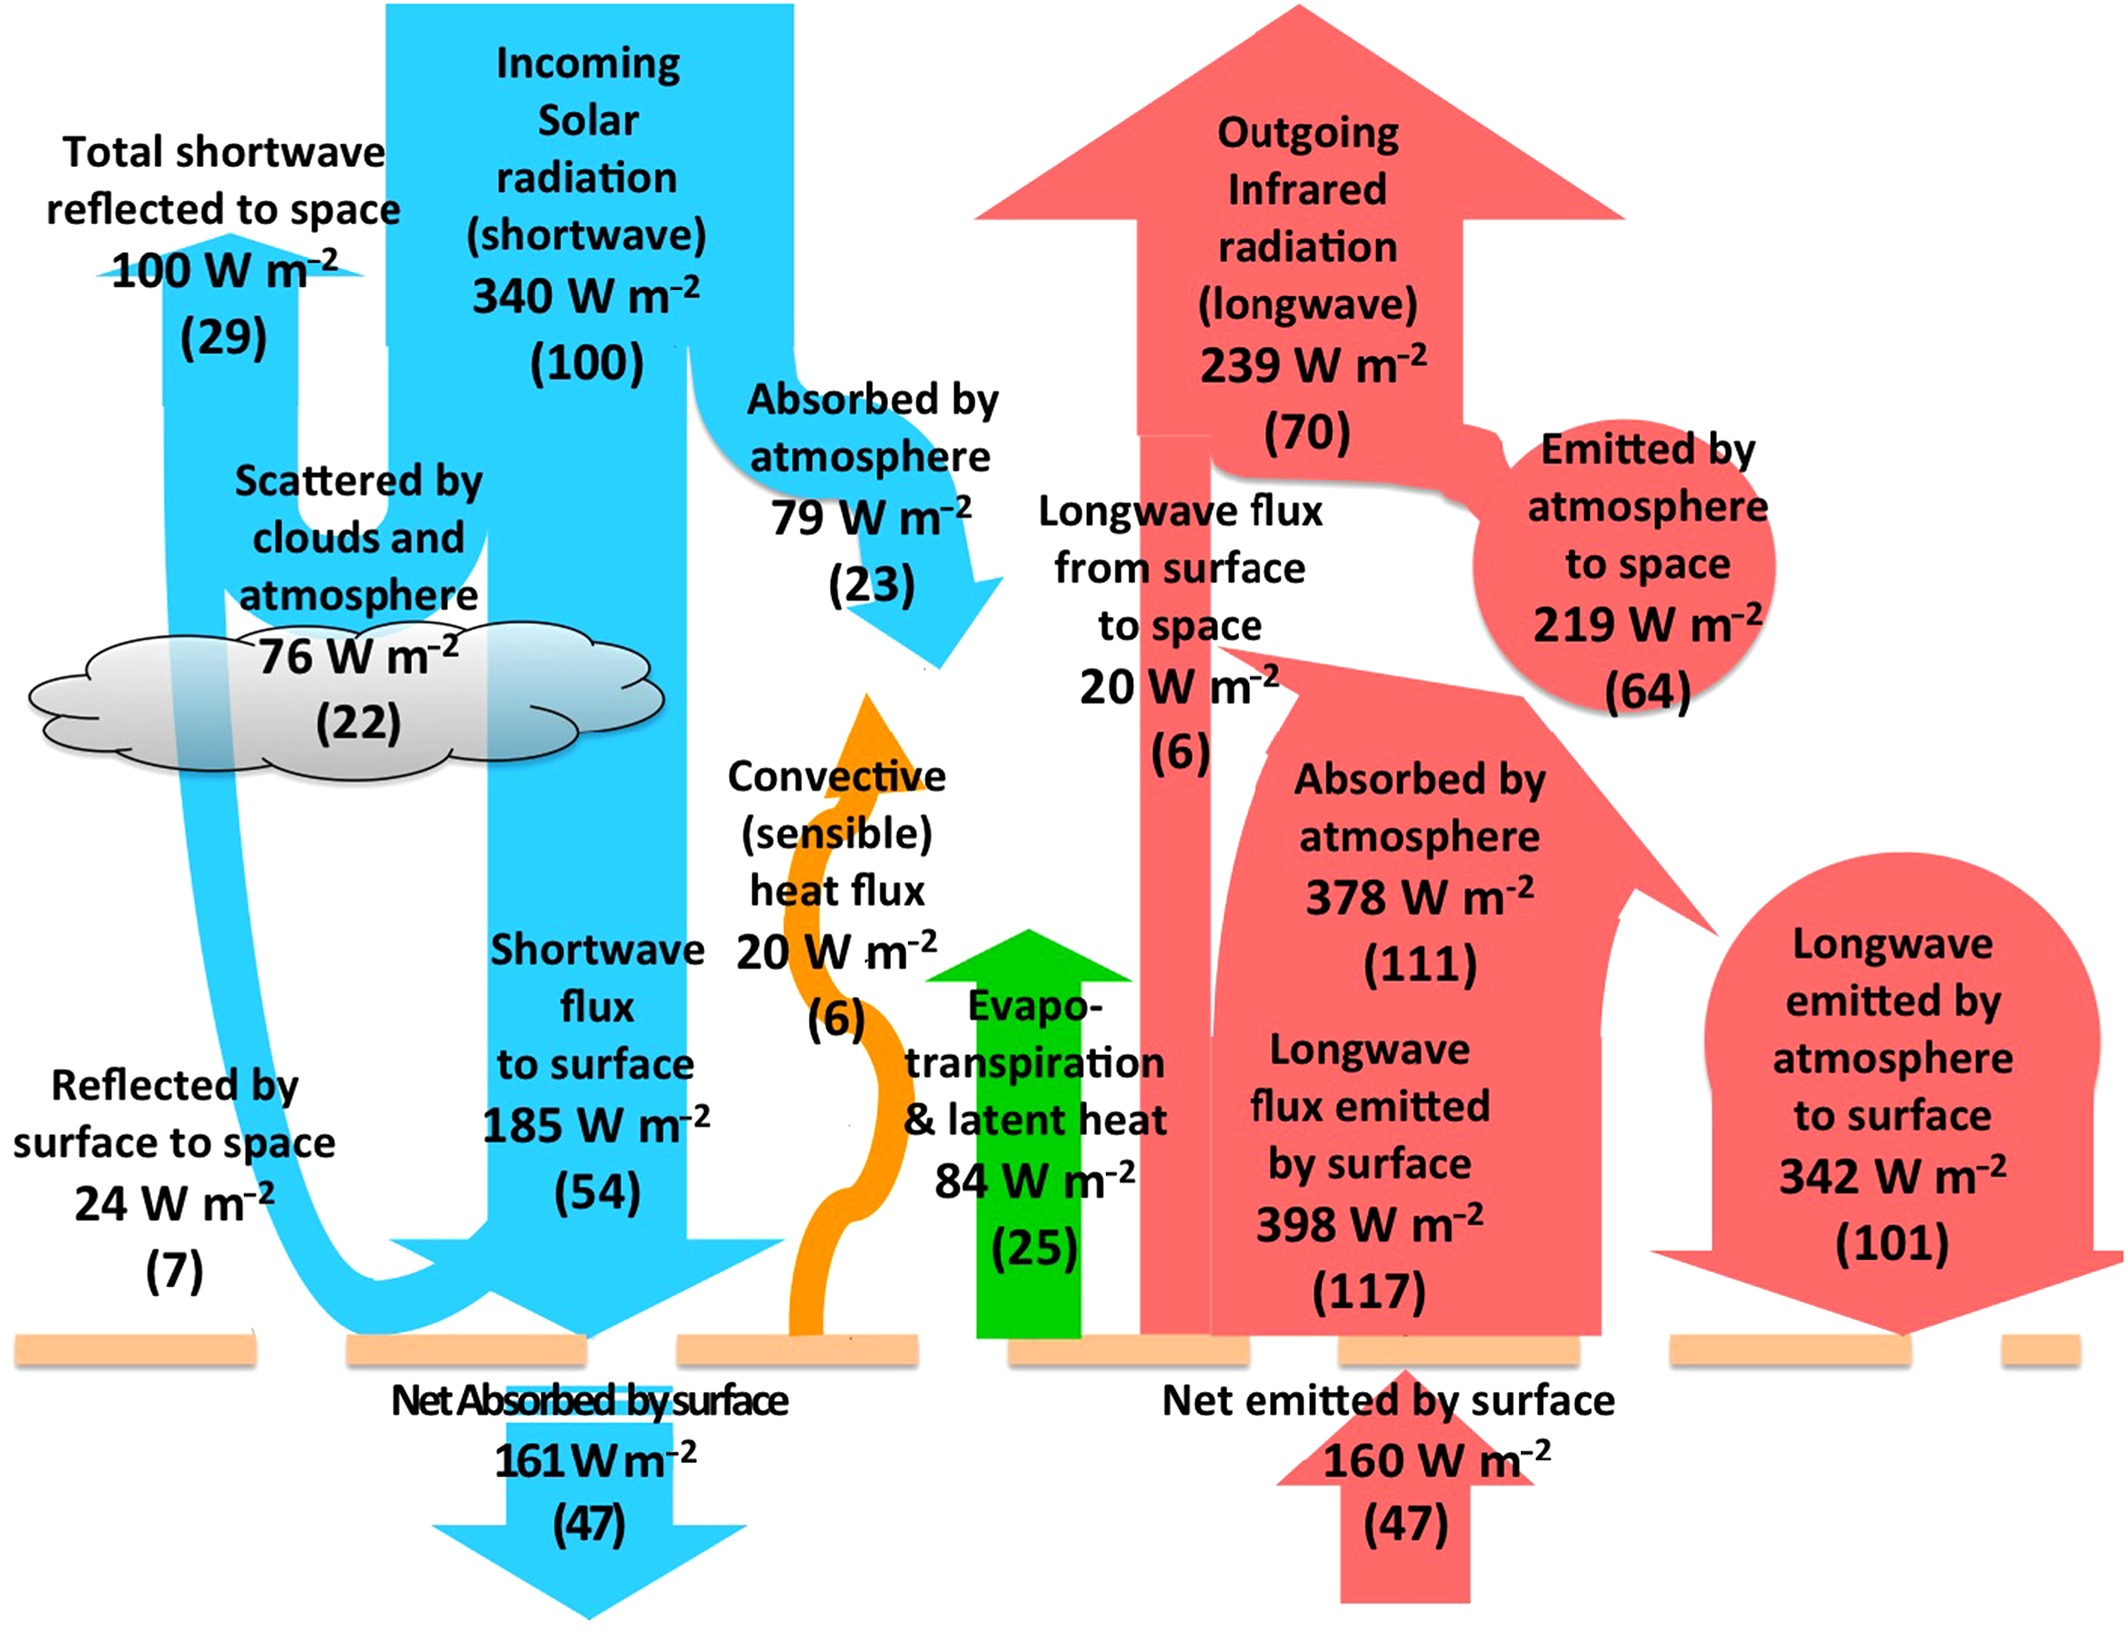
\includegraphics[width=0.7\columnwidth]{Chapter1/figs/01_trenberth.jpg}
    \caption[The Earth’s energy budget]{The Earth’s energy budget from \citet{readGlobalEnergyBudgets2016}, first used in \citet{kiehlEarthAnnualGlobal1997}}
    \label{fig:trenberth}
\end{figure}


There are many physical processes that affect the Earth's energy budget, with impacts at different times and spatial scales, such as increased carbon dioxide concentration and surface albedo change \citep{forsterEarthEnergyBudget2021}. A consistent way to characterize the behaviour of the climate system is therefore needed, ideally by using global-scale metrics on a common scale. One such metric is radiative forcing.

\subsection{Concept of radiative forcing}

Radiative forcing is a concept for quantifying the effects of physical processes that perturb the Earth's energy budget, connecting the effect of each individual perturbation to radiation changes and hence to global surface temperature response \citep{thornhillEffectiveRadiativeForcing2021}. The most recent IPCC report employs the definition of Effective Radiative Forcing (ERF) as the principal metric for quantifying such physical perturbations \citep{forsterEarthEnergyBudget2021}. 

In short, the global surface air temperature (GSAT) responds to a perturbation from a certain radiative forcing that gives rise to an energy imbalance at the top of atmosphere (TOA). This could be written as the linear energy budget equation.

\begin{equation}
\label{eq:erf}
    \Delta N = \Delta F - \alpha \Delta T
\end{equation}

Here, $\Delta N$ (W m$^{-2}$) denotes the change in the top-of-atmosphere net downward radiative flux, which is the result of the effective radiative forcing perturbation $\Delta F$ (W m$^{-2}$). $\alpha$ is the net feedback parameter and $\Delta T$ ($^\circ$C) is the change in global surface air temperature. 

Figure \ref{fig:1.ERF} shows the pre-industrial to present-day effective radiative forcing estimates for 1750 to 2019 for the concentration change in different forcing agents as featured in the Intergovernmental Panel on Climate Change (IPCC) assessment report (AR) 6 \citep{forsterEarthEnergyBudget2021}. Carbon dioxide (\ce{CO2}), ozone (\ce{O3}) and other well-mixed gases have positive radiative forcing, which means they exert a warming effect on global surface air temperature. In contrast, both aerosol-cloud and aerosol-radiation ERFs are negative. Moreover, aerosol effective radiative forcing also has the largest uncertainty of all forcings assessed in the IPCC report.

\begin{figure}
    \centering
    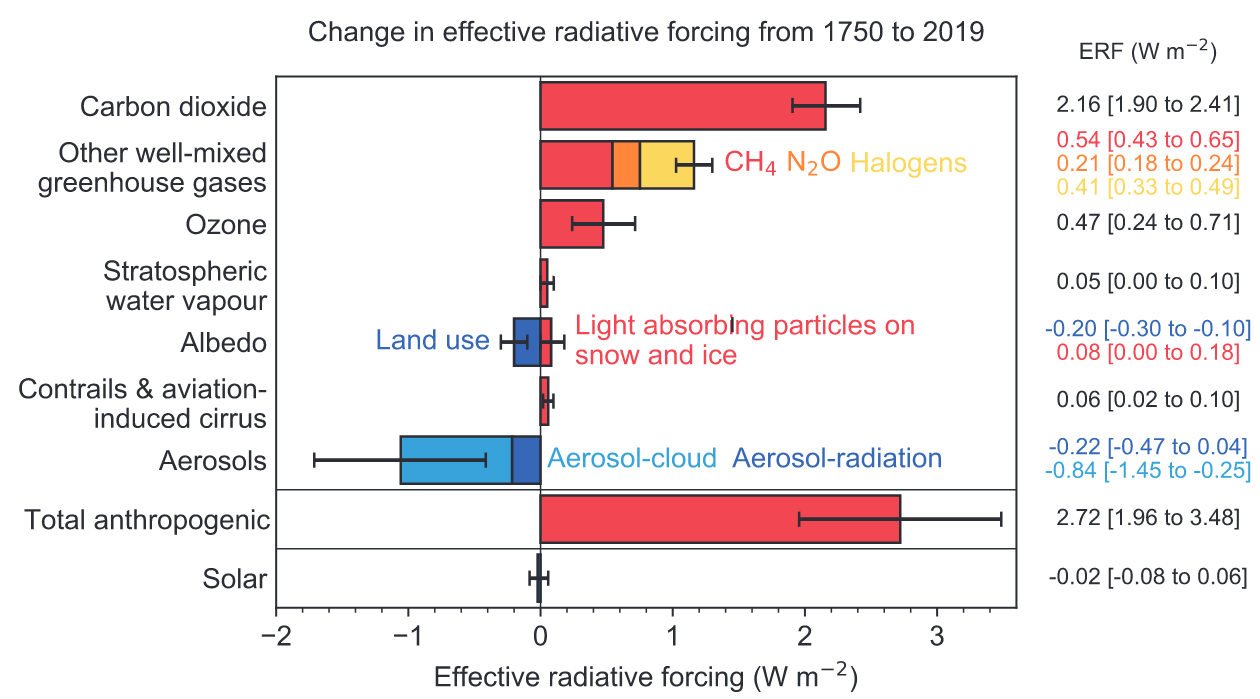
\includegraphics[width=6in]{Chapter1/figs/02_ERF.png}
    \caption[Effective radiative forcing (ERF) from 1750 to 2019]{Change in effective radiative forcing (ERF) from 1750 to 2019 by contributing forcing agents. Solid bars error bars represent best estimates and 5-95\% ranges. Figure from \citet{forsterEarthEnergyBudget2021}.}
    \label{fig:1.ERF}
\end{figure}

There are two approaches to evaluating ERF using climate simulations \citep[e.g.][]{gregoryNewMethodDiagnosing2004, oconnorAssessmentPreindustrialPresentday2021}.  The first method is to apply a step change to the forcing. This will immediately cause energy imbalance which will decrease as the system readjust itself back to the equilibrium ($\Delta N=0$). Equation \ref{eq:erf} gives the linear relationship between the annual global average temperature change to the annual energy imbalance. The linear relationship is assumed and the y-intercept is the value of ERF. This is usually referred to as the Gregory or the regression-based method \citep{gregoryNewMethodDiagnosing2004}. Another method is to set the $\Delta T$ term to zero. However, it is difficult to do so, so most studies prescribe sea surface temperature (SST) and sea ice concentration. A pair of simulations with and without the change in forcing is then performed for the fixed SST (fSST) simulations to estimate ERF as the difference in TOA radiative flux \citep{myhreNewEstimatesRadiative1998}. 


Effective radiative forcing is a good predictor of climate because the ratios of surface temperature change to forcing resulting from perturbations of different forcings are comparable \citep{myhreAnthropogenicNaturalRadiative2013, boucherCloudsAerosols2014}. One of the collaborative efforts to estimate effective radiative forcing from models is the CMIP which is detailed in section \ref{sec:1.CMIP6}


\subsection{Role of aerosol on climate}

The effective radiative forcing due to aerosols can be divided into aerosol-radiation interaction (ERFari) and aerosol-cloud interaction \citep[ERFaci;][]{ghanTechnicalNoteEstimating2013}. The aerosol direct effect, also referred to as aerosol-radiation interaction, can be observed locally e.g. from above the aerosol layer, such as from an aeroplane or from a mountaintop, as the layer scatters light, causing the appearance of a white or light-coloured hazy layer \citep{twomeyInfluencePollutionShortwave1977}. Such processes reduce solar radiation that reaches the Earth’s surface, with the optical depth depending on the total column mass burden of aerosol particles, but also on the size distribution and the particles’ optical properties. Not all types of aerosols scatter radiation with the same efficiency and some aerosols, such as soot, can also absorb solar radiation, as manifested in their naturally darker colour. 

The aerosol indirect effect, or aerosol-cloud interaction, encompasses the effects of aerosols on clouds and can be further divided into the effects of aerosol on cloud amount, cloud lifetime and cloud albedo.  Aerosols serve as cloud condensation nuclei and promote cloud formation \citep{albrechtAerosolsCloudMicrophysics1989}.  Changes in aerosol concentration are connected to variations in the cloud droplet size and number distribution. When there are more aerosols, cloud droplets are smaller. These clouds have less water content and appear brighter white, and, as a consequence, reflect more sunlight back to space, increasing planetary albedo. Examples of observed aerosol effects on the Earth’s atmosphere include volcanic aerosols \citep[e.g.][]{malavelleStrongConstraintsAerosol2017}, such as the 1991 eruption of Mount Pinatubo \citep{hansenPotentialClimateImpact1992}, and aerosols from ship tracks \citep{twohyEvaluationAerosolIndirect2005}. 



\section{Climate change and trends in short-lived climate forcers emissions and concentration}

% General idea of gases and pollutants that increase since PI
Anthropogenic emissions have generally increased since 1850 due to the accelerated industrialisation of the economy. This has led to an x-fold increase in methane emissions, an x-fold increase in CO2 both of which are greenhouse gases. 

% Specific increases of CH4 
Specific increases of CH4 

% idea of atmospheric oxidative power
idea of atmospheric oxidative power

% Changes to oxidants such as O3 and OH
Changes to oxidants such as O3 and OH

\section{Global tropospheric sulfur and sulfate aerosol budget}

Sulfate aerosol is emitted from both anthropogenic and natural sources, and is also produced from chemical production in the atmosphere by gas or aqueous phase reactions of sulfur dioxide (\ce{SO2}), dimethyl sulfide (DMS) and carbonyl sulfide \citep[OCS;][]{belvisoAssessmentMarineBiota2000}. After \ce{SO2} is released into the troposphere, it oxidises and forms sulfate aerosol.  The tropospheric sulfur cycle is closed by wet and dry deposition.

\begin{figure}
    \centering
    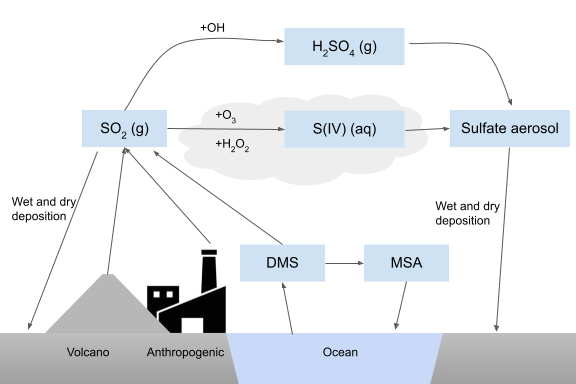
\includegraphics[width=6in]{Chapter1/figs/sulfur_budget.png}
    \caption[Summary of atmospheric sulfur budget]{Summary of atmospheric sulfur budget}
    \label{fig:sulfur-budget}
\end{figure}

\subsection{\ce{SO2} primary emission}

Primary emission of \ce{SO2} from natural sources comes from volcanic activities. Both continuously degassing volcanoes and sporadic eruptive volcanoes contribute to the Earth's tropospheric \ce{SO2} amount. Together, volcanic sources account for 2.251  Tg (S) yr$^{-1}$ between 1978--2014 \citep{carnMultidecadalSatelliteMeasurements2016}. Anthropogenic activities contribute to global sulfur emission mainly from industries and fossil fuel consumption for energy with the global emission of 50--70 Tg (S) yr$^{-1}$ \citep{forsterEarthEnergyBudget2021}. Secondary emission sources of \ce{SO2}  such as dimethyl sulfide (DMS) are discussed in section \ref{ch1:other-so2}.

Anthropogenic \ce{SO2} emissions are necessarily heterogeneous and localised \citep{manktelowRegionalGlobalTrends2007}. After large historical emissions centred in the US and Europe, decreasing trends were observed from North America and Europe, countered by increasing emissions from Eastern and Southern Asia, between 1980 and 2015 \citep{szopaShortlivedClimateForcers2021, aasGlobalRegionalTrends2019}. 




\subsection{\ce{SO2} oxidation}
\label{ch1:so2-oxidation}

In the atmosphere, \ce{SO2} can react with other gases, dissolve in a liquid droplet to undergo an aqueous reaction, or directly react with aerosol surfaces. In this section, we examine the formation routes of sulfate aerosol that are relevant to this study. 

\subsubsection{Gas-phase reaction}

The hydroxyl radical (OH) is one of the most widespread and reactive radicals in the atmosphere. In unpolluted air, OH is produced by the photolysis of ozone (\ce{O3}) and the subsequent reaction of oxygen atoms with water vapour \citep{wayneChemistryAtmospheresIntroduction2006}. In polluted air, the photolysis of nitrous acid (HONO) and hydrogen peroxide (\ce{H2O2}) yields OH directly. 

OH radical reacts rapidly with \ce{SO2} in the atmosphere through the reaction
\begin{align}
\ce{SO2 + OH + M -> HOSO2 + M}    
\label{ch1:eq:so2-oh}
\end{align}

Where M represents a molecule (usually \ce{N2}) that absorbs excess kinetic energy from the reactants. The free radical \ce{HOSO2} reacts in a chain of reactions with \ce{O2} and \ce{H2O} to form sulfuric acid, \ce{H2SO4}.
\begin{align}
\ce{HOSO2 + O2 &-> HO2 + SO3}\\
\ce{SO3 + H2O &-> H2SO4}
\end{align}

Once formed, \ce{H2SO4} (g) reacts with e.g. \ce{NH3}, amines, \ce{H2O} and nucleates into new aerosol particles \citep{seinfeldAtmosphericChemistryPhysics2016}.

\subsubsection{Aqueous-phase reaction}

\ce{SO2} can dissolve into liquid droplets, forming an equilibrium with its ionic products (\ce{SO2.H2O}), bisulfate ions (\ce{HSO3-}) and sulfite ions (\ce{SO3^2-}). \ce{SO2} and its oxidants dissolve into cloud droplets following the effective Henry's law \citep{seinfeldAtmosphericChemistryPhysics2016}: 

\begin{equation}
    H_i(T) = H_{i,298}\mathrm{exp} \bigg\{ -\frac{\Delta H_i}{R} \bigg( \frac{1}{T} - \frac{1}{298} \bigg) \bigg\}
\end{equation}

where $i$ is the species dissolved such as \ce{SO2}, \ce{O3} and \ce{H2O2}.  The constants take the following values: 
$H_{H_2O_2, 298}=7.45 \times 10^4 \mathrm{Matm}^{-1}$, 
$\Delta H_{H_2O_2} = 60.7 \times 10^3 \mathrm{Jmol}^{-1}$, 
$H_{O_3, 298}=1.13 \times 10^{-2} \mathrm{Matm}^{-1}$, 
$\Delta H_{O_3} = -21.1 \times 10^3 \mathrm{Jmol}^{-1}$, 
$H_{SO_2, 298}=1.23 \mathrm{Matm}^{-1}$, and
$\Delta H_{SO_2}=-26.1 \times 10^3 \mathrm{Jmol}^{-1}$. 
Hence, the concentrations of the species are given by

\begin{equation}
    \begin{aligned}
        \relax[\mathrm{H_2O_2}] & = H_{\mathrm{H_2O_2}}(T)p_{\mathrm{H_2O_2}} \\
        [\mathrm{O_3}] & = H_{\mathrm{O_3}}(T)p_{\mathrm{O_3}} \\
        [\mathrm{SO2}] & = H_{\mathrm{SO2}}(T)p_{\mathrm{SO_2}} \\
        [\mathrm{HSO_3^-}] & = \frac{K_{s,1}H_{\mathrm{SO_2}}(T)p_{\mathrm{SO_2}}}{[\mathrm{H^+}]}\\
        [\mathrm{SO_3^{2-}}] & = \frac{K_{s,2}[\mathrm{HSO_3^-}]}{[\mathrm{H^+}]}\\
    \end{aligned}
\end{equation}

where $p_i$ is the partial pressure of $i$,  
$K_{s,1} = 1.3 \times 10^{-2}$ M, and 
$K_{s,2} = 6.6 \times 10^{-8}$ M.  
These +4 oxidation state sulfur species undergo a chain of reactions to form +6 oxidation state species such as \ce{SO4^2-}. 
\begin{align}
    \ce{HSO3- + H2O2 &-> SO4^2-} \\
    \ce{HSO3- + O3 &-> SO4^2-} \\
    \ce{SO3^2- + O3 &-> SO4^2-} 
\end{align}

The rates of conversion of S(IV) to S(VI) via oxidation by \ce{H2O2} and \ce{O3} are calculated, respectively, as

\begin{align}
    \frac{d[\mathrm{S(VI)}]}{dt} & = [\mathrm{O_3}]( k_3 \mathrm{SO_2 \cdot H_2O} + k_4 [\mathrm{HSO_3^-}] + k_5 [\mathrm{SO_3^{2-}}]) \label{ch1:eq:so2-o3} \\
    \frac{d[\mathrm{S(VI)}]}{dt} & = \frac{k_1 \mathrm{[H^+][HSO_3^-][H_2O_2]}}{1+k_2[H^+]} \label{ch1:eq:so2-h2o2}
\end{align}

where 
$k_1 = 7.5 \times 10^7 \mathrm{M}^{-2}s^{-1}$,
$k_2 = 13 \mathrm{M}^{-1}$,
$k_3 = 2.4 \times 10^4 \mathrm{M}^{-1}s^{-1}$,
$k_4 = 3.7 \times 10^5 \mathrm{M}^{-1}s^{-1}$, and
$k_5 = 1.5 \times 10^9 \mathrm{M}^{-1}s^{-1}$. 

It has been observed that \ce{O3} reaction with sulfur-containing compounds is less effective when the aerosol pH is less than 4, while sulfur oxidation by hydrogen peroxide, which requires a proton (\ce{H+}) to form sulfate ions \citep{seinfeldAtmosphericChemistryPhysics2016}, is more efficient at lower pH. Thus the relative rate of these two reactions is regulated by the droplet pH. 

Aqueous phase reaction increases aerosol mass concentration via condensation onto existing aerosol particles, resulting in increased mass concentration but constant number concentration \citep{seinfeldAtmosphericChemistryPhysics2016}.


\subsection{\ce{SO2} deposition}

Removal of atmospheric trace gases can be described into two broad categories depending on the involvement of precipitation. Dry deposition refers to the process that removes gas or aerosol from the atmosphere onto the surfaces of the Earth, including oceans \citep{dewysAssessmentFateSulfur1978}.  Wet deposition describes the removal of gases and particles by incorporation into precipitation \citep{wayneChemistryAtmospheresIntroduction2006}. 

To undergo dry deposition, the trace gas must come into contact with the Earth's surface, such as tree foliage or the ground, via e.g. turbulent mixing, and be removed by some specific chemical or biological interaction.  Deposition velocities range from a few millimetres per second to a few centimetres \citep[e.g.][]{smithAirborneTransportSulphur1975, hardacreEvaluationSO2SO422021, mulcahyUKESM1DevelopmentEvaluation2022}.

Wet deposition is significant for gaseous compounds that are water-soluble. Less soluble compounds may react and form a more soluble compound before being wet-scavenged \citep{wayneChemistryAtmospheresIntroduction2006}. For example, \ce{SO2} gets oxidised, forming \ce{H2SO4}, before wet scavenging removes it from the atmosphere \citep{seinfeldAtmosphericChemistryPhysics2016}.


\subsection{Other sources of sulfur and secondary emission of \ce{SO2}}
\label{ch1:other-so2}

Biogenic processes emit sulfur in the reduced forms of \ce{H2S}, \ce{(CH3)2S} (dimethyl sulfide; DMS), and \ce{(CH3)2S2} (dimethyl disulfide). DMS is an important sulfur-bearing gas that is produced by algae in the oceans and is believed to be the source background of \ce{SO2} in the atmosphere. Sulfur-containing gases are oxidized into \ce{SO2} and are considered the secondary emission sources for \ce{SO2}, contributing 15--35 Tg(S) yr$^{-1}$ of \ce{SO2} globally \citep{lanaUpdatedClimatologySurface2011}.


\section{Global tropospheric sulfate aerosol chemical modelling} %Section - 1.2
\label{section1.2}

\subsection{First generation of global sulfur modelling}

The first sulfur aerosol global circulation model to consider a full annual cycle of sulfur was developed by \citet{langnerGlobalThreedimensionalModel1991}, representing three-dimensional atmospheric transport together with a sulfur cycle to study the global distribution of sulfur compounds. Preceding works were either two-dimensional model (latitude-height) models \citep{rodheGlobalDistributionSulfur1980} or only emphasised the aerosol formation aspect and oversimplified the sulfur reaction pathways \citep{ericksoniiiGlobalOceantoatmosphereDimethyl1990}. The work of \citet{langnerGlobalThreedimensionalModel1991} included three sulfur species: DMS emitted from natural sources as gases, \ce{SO2} as gases from both natural and anthropogenic sources, and \ce{SO4^2-} as aerosols where most of the emission occurs as DMS or \ce{SO2}. In the model, these species react via gas- and aqueous-phase reactions with prescribed reaction rates that are either constant across the globe or are zonally averaged, with \ce{SO4} as the end product of the oxidation process. For the aqueous-phase reactions which require the presence of clouds, prescribed climatological cloud cover was used. Removal processes were implemented for both wet and dry deposition using parameterized rates that depended on all spatial and temporal dimensions. The three sulfate species are transported within the model with resolution of $10^\circ$ latitude by $10^\circ$ longitude and 10 vertical layers. These were integrated with a one-hour timestep with 5 months spin-up and 12 months of model output for analysis. Despite the many limitations, \citet{langnerGlobalThreedimensionalModel1991} achieved a broad consistency with available observed concentrations, especially in polluted regions such as Northern America and Europe.

In the following decade, the complexity of atmospheric sulfur modelling increased, and sulfate species reactions were embedded into general circulation models and into other chemical transport models \citep[e.g.][]{kochTroposphericSulfurSimulation1999}.  In 2001, the first aerosol model intercomparison, the COmparison of large-scale atmospheric Sulfate Aerosol Model or COSAM, was performed  \citep{barrieComparisonLargescaleAtmospheric2001, lohmannVerticalDistributionsSulfur2001, roelofsAnalysisRegionalBudgets2001}. This comparison project’s main goal was to “compare the ability of the current model to simulate spatial/temporal distribution of aerosol” \citep{barrieComparisonLargescaleAtmospheric2001}. Hence, the aerosol effects on the Earth’s climate were not their main focus.  Out of 11 models that participated in COSAM, 3 of which were general circulation models (GCMs) which solved their own meteorological fields such as wind and cloud. COSAM found that models predicted surface level seasonal mean mixing ratio of \ce{SO4} better than \ce{SO2} which suggested that vertical mixing in emission source regions was a major reason for prediction uncertainty \citep{lohmannVerticalDistributionsSulfur2001}. 

One of these three GCMs was the Goddard Institute for Space Studies general circulation model (GISS GCM) which included the following prognostic species: \ce{SO2}, sulfate, hydrogen peroxide (\ce{H2O2}), DMS and methanesulfonic (MSA), and was capable of estimating sulfate aerosol direct effect on the Earth’s radiative budget \citep{kochTroposphericSulfurSimulation1999}. A study using this model highlighted a relatively minor role for online chemistry in estimating radiative forcing: running the model using climatological sea surface temperatures and comparing two experiments, one with online chemistry and one with offline chemistry, showed little difference between offline and online models in the global average but did show that as great as 10\% differences in polluted regions resulted in the offline and online chemistry experiments.

By 2005, most models used one of two approaches to simulate the sulfur cycle: using offline meteorology and online chemistry inside a chemical transport model (CTM), or using prescribed aerosol for calculating radiative forcing in a GCM.  In their 2005 review, \citet{lohmannGlobalIndirectAerosol2005} stated that global model estimates of aerosol direct and indirect effects were highly uncertain. 

By 2010, \citet{tsaiSulfurCycleSulfate2010} had incorporated tropospheric sulfur chemistry into a global climate model, aiming to estimate the radiative forcing of direct and indirect aerosol effects. The result is interactive tropospheric sulfur chemistry within a global climate model. Other research centres followed this development.

\subsection{State of the science in sulfur modelling}

Earth system models have become more complex and include more components since the first global transport-chemistry model developed by \citet{langnerGlobalThreedimensionalModel1991}. Climate models now routinely feature online, that is prognosed, aerosol formation processes and modelling capability has increased steadily in complexity to the current state of the art in the 6th Phase of the Coupled Model Intercomparison Project \citep[CMIP6, details in next section;][]{eyringOverviewCoupledModel2016}. 

Many of the CMIP6 models feature coupled atmosphere-ocean free-running climate models which feature online chemistry and sulfate aerosol, albeit with varying levels of sophistication in the treatment of aerosol-cloud-radiation interactions \citep[e.g.][]{zhangBCCESM1ModelDatasets2021, vannoijeECEarth3AerChemGlobalClimate2021, mulcahyDescriptionEvaluationAerosol2020}.  Aerosol microphysics is typically treated using single-moment schemes, in which a single tendency of mass or aerosol number alone is calculated, or two-moment schemes, in which both the mass and the total number concentration of aerosols are predicted.  Accurate treatment of short time- or spatial-scale aerosol-cloud interactions, such as freezing, coagulation and coalescence are usually parameterised. Cloud formation and latent heat release affect atmospheric circulation.  Aerosols also connect to hydrology via their effect on precipitation \citep{allenInterhemisphericAerosolRadiative2015}. In essence, aerosols couple into atmospheric circulation through their effect on surface radiation, modifying sea-surface temperatures (and hence evaporation \citep{boothAerosolsImplicatedPrime2012}) and potentially ocean circulation \citep{cowanResponseLargescaleOcean2013}. These strong effects, together with the uncertainty in their various responses, lead to varying levels of confidence in our ability to understand how aerosol radiative forcing has changed and will evolve in the future.


With respect to aerosol processes, there have been some improvements to sulfate aerosol modelling in IPCC AR6 since the previous assessment \citep{forsterEarthEnergyBudget2021}. Some models include pH dependency of \ce{SO2} oxidation \citep[such as the NorESM1;][]{kirkevagProductiontaggedAerosolModule2018} and explicit descriptions of ammonium and nitrate aerosol components as studied by the Aerosol Comparisons between Observations and Models (AeroCom) phase III \citep{bianInvestigationGlobalParticulate2017}.


Despite the known effect of aerosol on atmospheric chemistry \citep[e.g.][]{oconnorApportionmentPreIndustrial2022}, sulfate aerosol modelling is still an active area of study with many open questions. For example, as the large number of chemical species slows down the progress of the study due to computational resource limits, there remain gaps in treatment of aerosol composition (e.g. nitrate, secondary organic aerosols) in many regions \citep[e.g.][]{mulcahyDescriptionEvaluationAerosol2020}, and parameterizations of sub-grid processes add to the uncertainty of model prediction so that much of the feedback between aerosol and other components of the Earth system is not yet fully explored \citep{seikiImprovementGlobalCloudSystemResolving2015}. This project aims to address some of these questions such as the effects of atmospheric composition and oxidant changes on aerosol radiative forcing.



\section{Surface temperature anomalous cooling in UKESM1 CMIP6 experiments}

\begin{figure}
    \centering
    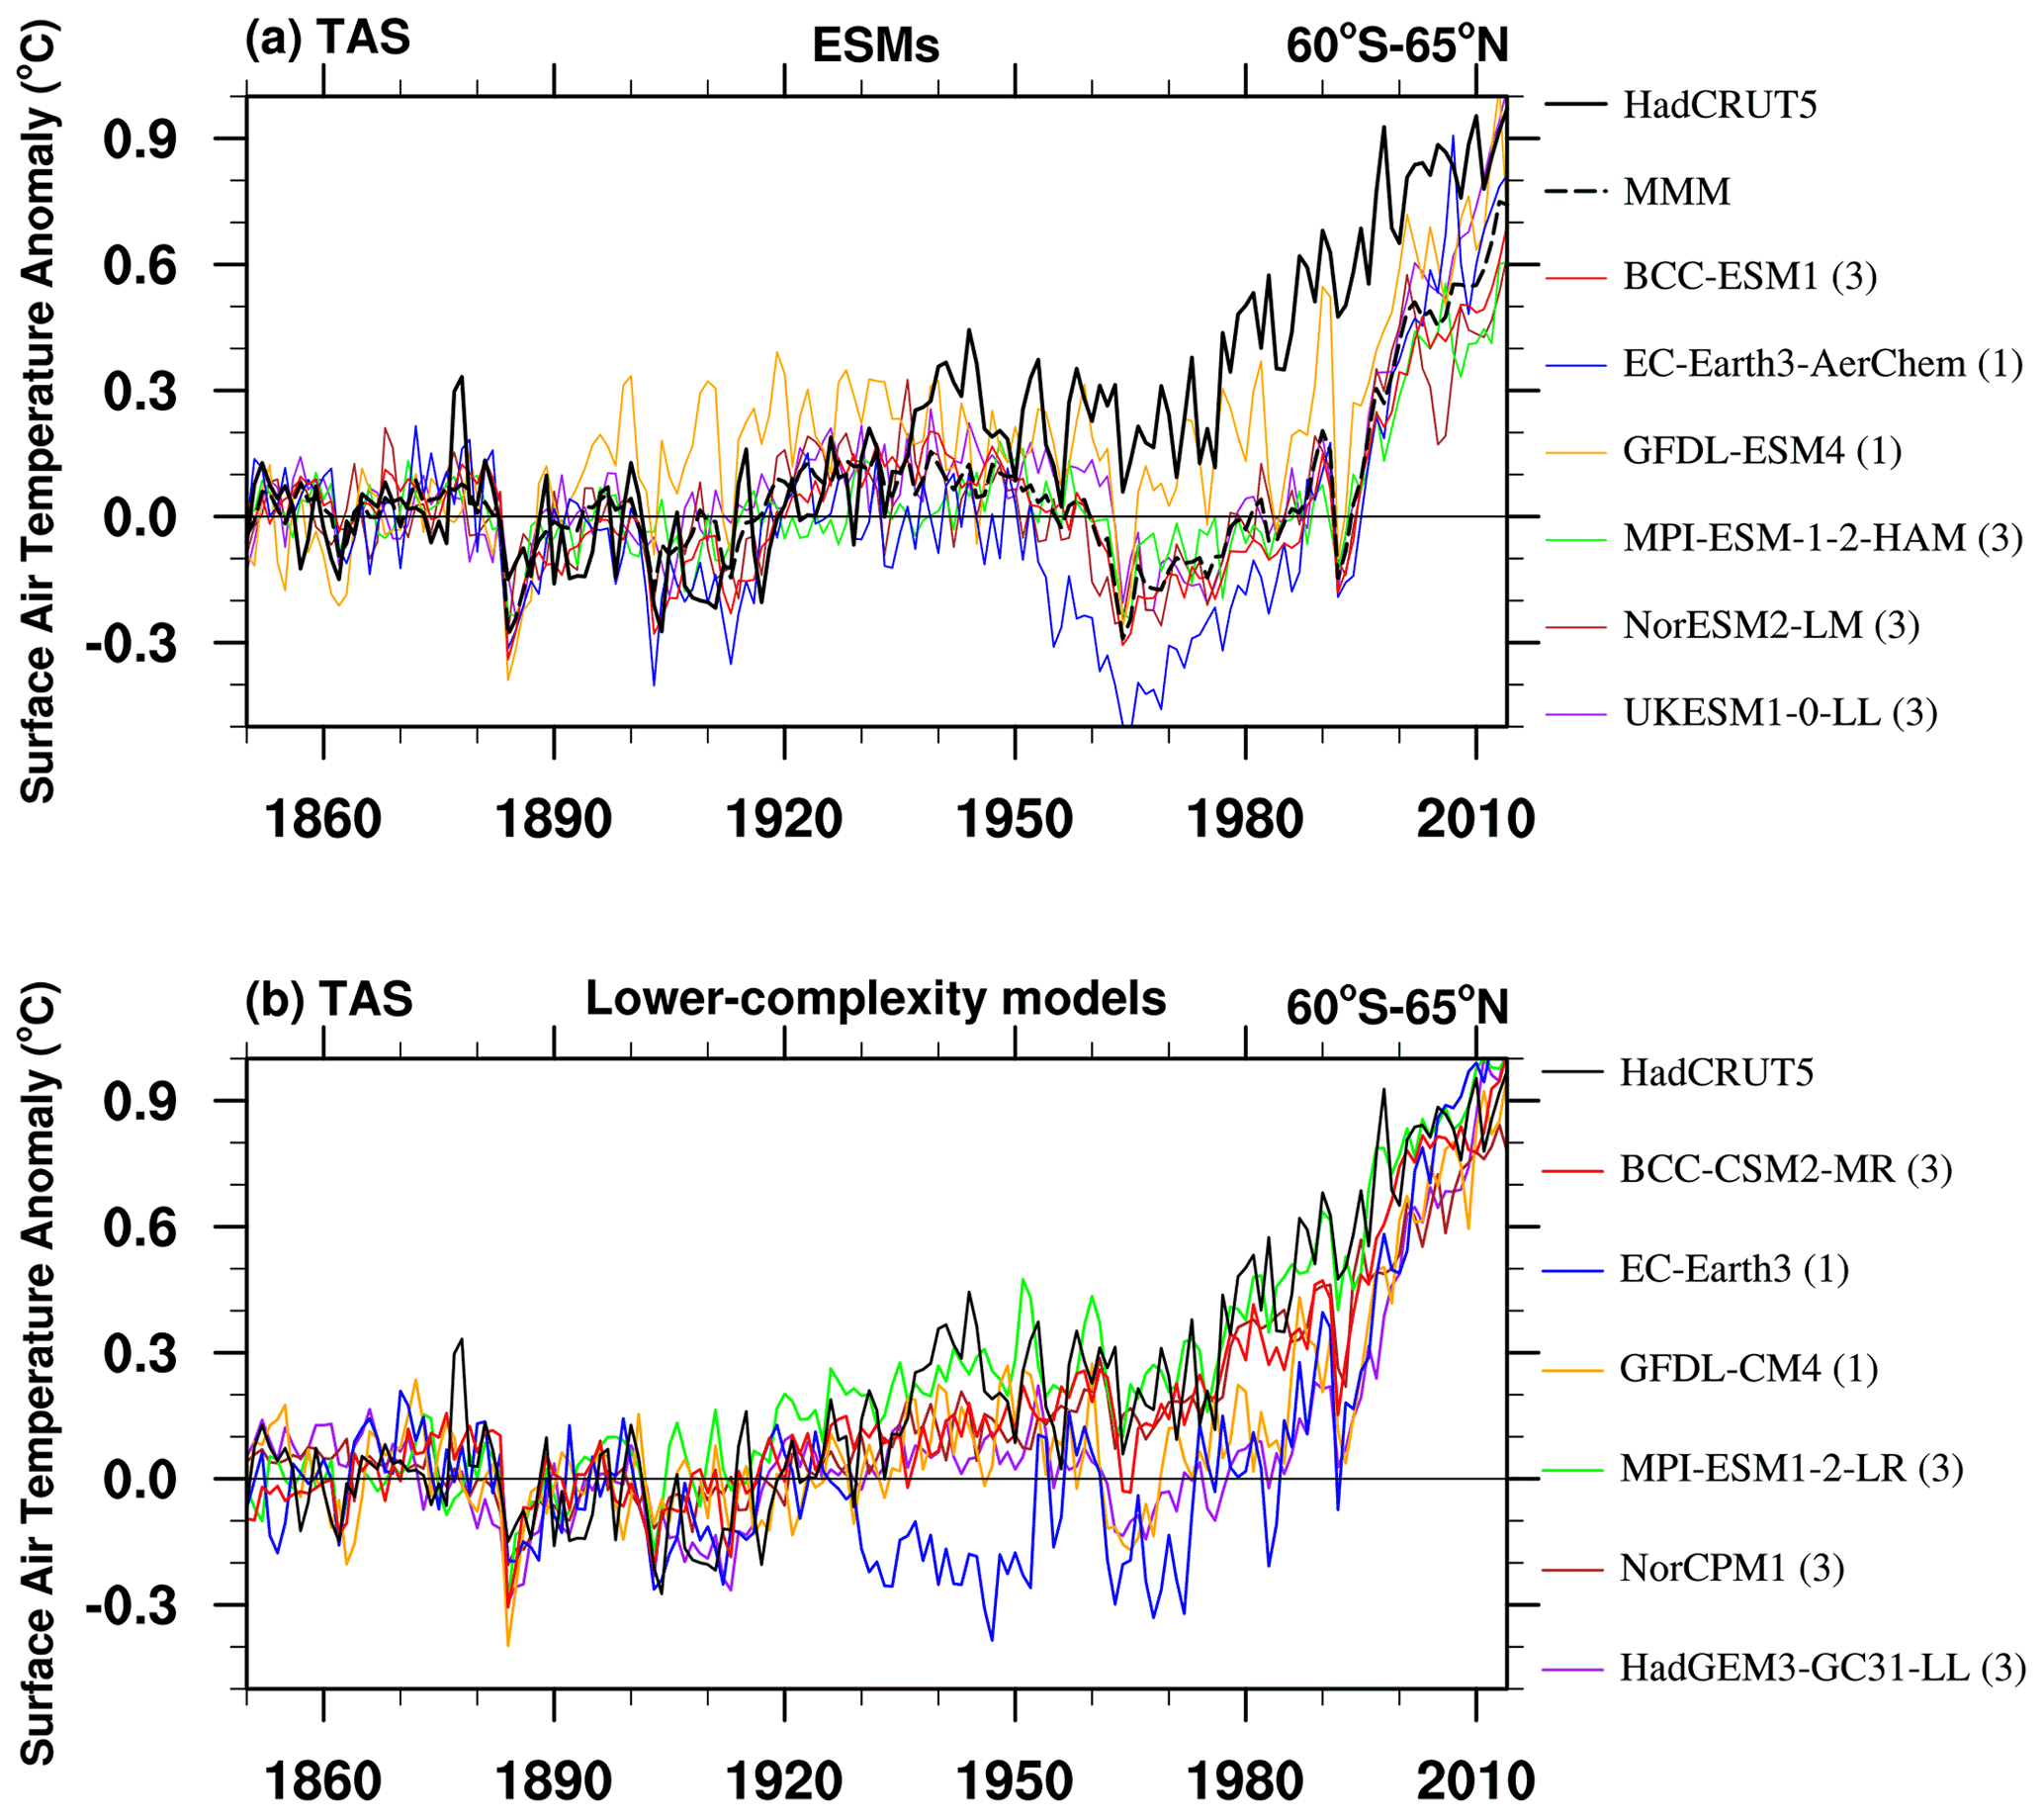
\includegraphics[width=6in]{Chapter1/figs/pothole_figure_Zhang2021.png}
    \caption[Anomalous cooling in the Earth system models participating in CMIP6]{(a) Historical near-global mean (60$^\circ$ S to 60$^\circ$ N) surface air temperature anomalies relative to 1850--1900 surface air temperature (TAS) from HadCRUT5 (thick black line), the ensemble mean for each ESM (solid colour lines), and multi-model mean (MMM, dashed black line). Panel (b) is the same as panel (a) but for the lower-complexity models. Units: $^\circ$C. Value in bracket is the number of available members for each model. \citep{zhangRoleAnthropogenicAerosols2021}.}
    \label{fig:zhang-pothole}
\end{figure}

In CMIP5, two separate configurations of the Met Office Unified Model were used. HadGEM3, being a coupled model with simplified, offline chemistry, participated in the historical simulations for CMIP5 climate projections,  while the UKCA chemistry-climate model, run in atmosphere-only mode but with online chemistry, took part in the Atmospheric Chemistry and Climate Model Intercomparison Project (ACCMIP) focusing on chemistry-climate interactions. The UKESM1 developed for CMIP6, brought online chemistry into a coupled atmosphere-ocean model, having been developed from the Met Office Unified Model and UKCA with the addition of Earth system modules.


The study by \citet{zhangRoleAnthropogenicAerosols2021} indicated that 6 models, table \ref{tab:zhang-model}, that participated in the CMIP6 tended to underestimate surface air temperature (TAS) during the period 1960--1990, known as the “pothole” period. This period coincided with elevated industrial activities over the Northern Hemisphere, especially in the Western European region. \ce{SO2} emitted by these industrial activities was one of the precursors of atmospheric sulfate aerosols which cooled down the atmosphere via aerosol direct and indirect effects. By comparing historical simulations with and without anthropogenic aerosol precursor emission, the study showed that anthropogenic emission led to more aerosol generation, with aerosol-cloud interaction accounting for up to 87\% of the aerosol forcing sensitivity. In addition, the study also indicated that the UKESM1 has the largest aerosol forcing sensitivity. 


\begin{small}
\begin{longtable}{>{\raggedright}p{3.25cm} >{\raggedright}p{3.25cm} >{\raggedright}p{3.5cm} >{\raggedright\arraybackslash}p{3.5cm}}
    \caption[Information of models included in the study by \citet{zhangRoleAnthropogenicAerosols2021}]{Information of models included in the study by \citet{zhangRoleAnthropogenicAerosols2021}}
    \label{tab:zhang-model}
    \\
    \toprule
     Model developer (Model) & Tropospheric chemistry model & Sulfur chemistry scheme & Aerosol scheme \\
     \midrule
     \endfirsthead

    \toprule
     Model developer (Model) & Tropospheric chemistry model & Sulfur chemistry scheme & Aerosol scheme \\
     \midrule
     \endhead
     
     \bottomrule
     \endlastfoot

     
     Met Office’s Hadley Centre for Climate Prediction and Research; MOHC (UKESM1-0-LL) Ref. \citet{sellarUKESM1DescriptionEvaluation2019,archibaldDescriptionEvaluationUKCA2020,mulcahyDescriptionEvaluationAerosol2020}  & UKCA (United Kingdom Chemistry and Aerosol) model with unified stratospheric-tropospheric chemistry (StratTrop) & Prognostic oxidant fields. Prognostic sulfur chemistry. & Aerosol scheme GLOMAP-mode. Two-moment, five size modes. 4 species: sulfate (\ce{SO4}), black carbon (BC), organic matter (OM) and sea salt. \\
     \midrule
     Norwegian Climate Center; NCC (NorESM2-LM). Ref. \citet{kirkevagProductiontaggedAerosolModule2018, selandOverviewNorwegianEarth2020} & Atmosphere model component CAM6-Nor built improvements on the CAM6 version from CESM2.1 & Diagnostic tropospheric oxidant fields: OH, \ce{O3}, \ce{H2O2}.  Prognostic  sulfur chemistry & 4 aerosol modes. 6 species: SOA, BC, \ce{SO4}, OM, Seasalt, and dust.  \\ 
     \midrule
     Max Planck Institute for Meteorology; MPI (MPI-ESM-1-2-HAM) Ref. \citet{neubauerGlobalAerosolClimate2019,neubauerHAMMOZConsortiumMPIESM12HAM2019,tegenGlobalAerosolClimate2019} & Atmospheric Model Component ECHAM6.3. &  Diagnostic oxidant fields: OH, \ce{H2O2}, \ce{NO2}, \ce{O3}, and \ce{NO3}. Prognostic sulfur chemistry. & Aerosol scheme HAM2.3. Two-moment. 7 modes: 4 soluble and 3 insoluble \\
     \midrule
     US Department of Commerce/ NOAA/Geophysical Fluid Dynamics Laboratory; GFDL (GFDL-ESM4) Ref. \citet{zhaoGFDLGlobalAtmosphere2018, heldStructurePerformanceGFDL2019, dunneGFDLEarthSystem2020} & Atmospheric component AM4.1 & Prognostic oxidant fields: OH, \ce{O3}, \ce{H2O2}, \ce{NO3}. Prognostic sulfur chemistry. & 5 aerosol types: sulfate, dust, black carbon, organic carbon, and sea salt.  \\
     \midrule
     European consortium of meteorological services, research institutes, and high-performance computing centers (EC-Earth-AerChem) Ref. \citet{vannoijeECEarth3AerChemGlobalClimate2021} & Aerosols and atmospheric chemistry are simulated with the Tracer Model version 5 (TM5), specifically release 3.0 of the massively parallel version of TM5 (TM5-mp 3.0). & The model includes aqueous-phase reactions for the oxidation of total dissolved sulfur dioxide & Modal aerosol microphysical scheme M7. 5 aerosol types: \ce{SO4}, BC, OA, sea salt, and mineral dust. 7 modes: 4 water-soluble and 3 insoluble modes  \\
     \midrule
     Beijing Climate Center; BCC (BCC-ESM1) Ref. \citet{zhangBCCESM1ModelDatasets2021} &  Atmospheric component is BCCAGCM3-Chem based on MOZART2 & Prognostic oxidant fields. Prognostic sulfur chemistry. & 5 aerosol species: \ce{SO4}, OC, BC, soil dust, and sea salt \\


\end{longtable}
\end{small}

One aspect of the historical experiment that remains of interest is the impact of emission migration equatorward and eastward in the last century and its implication and current state of understanding. Industrialization has led to rapid increases in greenhouse gas emissions along with aerosol precursors in many locations. The Industrial Revolution started in the Western European region with anthropogenic emissions peaking in 1980 followed by other regions such as the Indian subcontinent and Eastern Asia. It could be said that anthropogenic emissions have shifted eastwards and equatorward in the last 50 years.  \citet{zhangTroposphericOzoneChange2016} studied the effect of ozone precursor emission redistribution over the period 1980 to 2010 using climate models. The study separated the change in the magnitude of ozone precursor emission from the shift in emission location and concluded that the global tropospheric ozone change in this period is mainly due to the shift in the emission region rather than the magnitude of emission. Hence, the atmosphere is sensitive to emission location. Whether aerosol precursor emission migration which concurred with ozone precursor migration would lead to the same effect as ozone is not yet determined, and will be the focus of my work in the next six months.



\section{Aims and research questions}

Along with investigating the role of atmospheric chemistry in climate models, the overarching question of this work is to investigate the anomalous cooling period in the ESM by investigation of the \ce{SO2} oxidation pathways. Although \citet{zhangRoleAnthropogenicAerosols2021} identified the positive correlation between anomalous cooling and sulfate loading, the chemical and physical processes that lead to the overestimation of aerosol loading during the cooling period have not been identified. Identifying the processes and/or interactions within the climate model will improve future prediction capacity and reduce the uncertainty in aerosol forcing calculation. In addition, this project seeks to understand the effects of cloud droplets' pH on aerosol formation and radiative forcing and how pH affects model performance. 

In detail, this research aims to answer the following questions with respective aims and objectives.

\begin{enumerate}
    \item  How do \ce{SO2} budget and oxidation tendencies respond to changes in oxidant levels over the historical period?
    \begin{itemize}
        \item To understand the sulfate formation processes, the first part of this project focuses on sulfate chemistry in UKESM1 over the historical period. This work aims to utilise the data available from the CMIP6 and its endorsed project such as the AerChemMIP to study sulfate aerosols formation.  
        \item Sulfate production involves \ce{SO2} reaction with other precursors such as \ce{O3}, OH, and \ce{H2O2}. This part explores the global trends of sulfur budget and oxidation tendencies. It takes AerChemMIP transient experiments that perturb the oxidant levels such as \textit{histSST}, \textit{histSST-piO3}, etc., and investigates model sensitivity to oxidant changes. 
    \end{itemize}

    \item How does sulfate aerosol size distribution respond to oxidant perturbation?

    \begin{itemize}
        \item Oxidant level changes will have a knock-on effect on aerosol formation since \ce{SO2} oxidation forms aerosol and this process depends on the oxidant availability. The transient historical prescribed SST simulations from the AerChemMIP are useful for studying the attribution of climatic changes to precursor emissions. This section aims to quantify aerosol size distribution changes caused by oxidant level changes by comparing transient historical prescribed SST simulations experiments with the controlled \textit{histSST} experiment. 
    \end{itemize}

    \item At the process level, how do oxidant changes affect aerosol radiative forcing due to changes in oxidants?

    \begin{itemize}
        \item Aerosol radiative forcing is an important climate forcing with the largest uncertainty in the IPCC AR6 assessment. Building on our understanding of the underpinning aerosol production channels and sulfate burden, this part explores the climatic responses due to oxidant changes. 
    \end{itemize}

    \item How do changes in seasonal levels of oxidants affect aerosol formation and subsequent radiative effects?

    \begin{itemize}
        \item There are observed seasonal trends in oxidants from measurement and modelling studies.
        \item The UKESM1 can simulate both aerosol mass and number independently, making it one of the most robust climate models regarding aerosol simulation. GLOMAP-mode which is the aerosol module used in UKESM1 simulates both soluble and insoluble aerosols in four modes: nucleation, Aitken, accumulation and coarse and different aerosol types: sulfate, sea salt, organic, dust and black carbon. It also simulates interaction between modes such as coagulation and condensation as well as wet and dry deposition. This makes the UKESM1 a useful tool for studying the aerosol properties in different seasons.
    \end{itemize}

    \item The emission of aerosol precursors shifted eastwards and equatorward away from the European region since 1980. What is the effect of emission location change on oxidation tendencies?

    \begin{itemize}
        \item This part of the project explores regional sulfate formation and regional differences due to chemical background. In the historical period, anthropogenic emissions, including \ce{SO2}, increased with industrial activities in the European region and peaked in 1980 before decreasing. Then, emissions increased in Eastern Asia and reached their peak in the 200s. Since \ce{SO2} emission location dictates the background of available precursors and the atmospheric chemistry condition near the equator differs from that of the extratropical region, it is possible that different regions have different baseline oxidation tendencies and also behave differently to oxidant level changes. This section builds on Research Question 1 and further inspects the details in regions, aiming to find out the characteristics of oxidation in different time periods and regions.  
    \end{itemize}

    \item How does discrepancy in oxidant field affect aerosol formation and subsequent radiative effects?

    \begin{itemize}
        \item  We have access to an offline oxidant version of UKESM1, prepared by Alistair Sellar at UK Met Office, and to the data from the first sensitivity histSST experiments in which UKESM1 oxidants were replaced by those from analogous CESM2 experiments.  I plan to investigate the sulfur budget in these experiments, and to quantify the differences in both oxidant field and oxidant chemistry to determine the sensitivity of the aerosol chemistry to the oxidant fields in a way that complements the approach taken in Chapter 3 where \textit{histSST-piO3} and other experiments were analysed. To connect oxidant changes to ERF, we would need to set up other timeslice experiments. This work could be extended to investigate aspects of the radiative forcing such as the role of oxidant in ERFaci and other climate diagnostics. 
    \end{itemize}
    
\end{enumerate}

\section{Thesis structure and publication work}

Firstly, this thesis describes the work in preparation for publication which quantifies the role of SLCFs including methane and ozone precursors in modifying radiative balance through changes in aerosol formation (Chapter \ref{ch3}). Secondly, I describe how the seasonal cycle modifies SO2 oxidation and changes the radiative effects. Thirdly, oxidation is explored in the view of regional changes and its contribution to regional cooling. Finally, the sensitivity of SO2 oxidation to oxidants is explored in the final chapter.
%!TEX root = ../thesis.tex
%*******************************************************************************
%****************************** Second Chapter *********************************
%*******************************************************************************

\chapter{Data and Methods}

\ifpdf
    \graphicspath{{Chapter2/Figs/Raster/}{Chapter2/Figs/PDF/}{Chapter2/Figs/}}
\else
    \graphicspath{{Chapter2/Figs/Vector/}{Chapter2/Figs/}}
\fi

\section{CMIP6 and AerChemMIP experiment design}

This research focuses on \ce{SO2} oxidation and aerosol formation and utilizes data from the AerChemMIP transient historical atmosphere-only prescribed SST simulations \citep{collinsAerChemMIPQuantifyingEffects2017}. These simulations were designed to calculate transient ERFs that drive climate change.  While the simulations were not precisely designed for the purpose of this research, their configurations and emissions align well this research purpose.


Table \ref{tab:2.exps} shows the simulation configurations with all historical transient experiments from AerChemMIP that experiments cover the period between 1850 and 2014. "AOGCM" means atmosphere-ocean coupled simulation. "AGCM" means atmosphere-only simulation. The "AER" suffix means the models should at least calculate tropospheric aerosol driven by emission fluxes. The "CHEM$^\text{S}$" suffix means at least stratospheric chemistry is required; "CHEM$^\text{T}$" means at least tropospheric chemistry is required. "Hist" means the concentration or emission should evolve as for the CMIP historical simulation. "1850" means the concentrations or emissions should be fixed to the year 1850. 

\begin{table}
   \caption[AerChemMIP experiments related to this work]{A summary of AerChemMIP experiments related to this work.}
   \label{tab:2.exps}
   \centering
   \begin{tabular}{l p{30mm} l p{18mm} p{18mm} l}
    \toprule
     Experiment ID & Minimum model configuration & \ce{CH4} & Aerosol precursors & \ce{O3} precursors & suite-id \\
    \midrule
     \textit{historical}      & AOGCM AER & Hist & Hist & Hist & u-bc179\\
     \textit{hist-piAer}      & AOGCM AER & Hist & 1850 & Hist & u-bg705\\
     \textit{hist-piNTCF}     & AOGCM AER & Hist & 1850 & 1850 & u-bg946\\
     \textit{histSST}         & AGCM AER & Hist & Hist & Hist & u-bh626\\
     \textit{histSST-piAer}   & AGCM AER & Hist & 1850 & Hist & u-bi541\\
     \textit{histSST-piO3}    & AGCM CHEM$^{\text{T}}$ & Hist & Hist & 1850 & u-bl670\\
     \textit{histSST-piCH4}   & AGCM CHEM$^{\text{T/S}}$ & 1850 & Hist & Hist & u-bl551\\
     \textit{histSST-piNTCF}  & AGCM AER & Hist & 1850 & 1850 & u-bl277\\
     \bottomrule
   \end{tabular}
\end{table}

The CMIP6 requires that participating models archives a standardized set of variables that are processed in  specific ways. For example, the AerChemMIP archives sulfate aerosol formation tendency in two variables: \texttt{cheaqpso4} and \texttt{chegpso4}. These are the aqueous- and gas-phase production rate of \ce{SO4}, respectively. While this is useful for model intercomparison studies, \ce{O3} and \ce{H2O2} oxidation are added up to \texttt{cheaqpso4}, making it impossible to perform analysis based on individual channels. As such, the native model data is more useful for in-depth analysis specific to a model. This project uses both the processed AerChemMIP archive and UKESM1 native data.


\section{Definitions of terms and methods}
\label{sec:2.terms}
The main definitions used in this work are related to the concept of atmospheric chemical budget. The budget of a trace gas consists of three quantities: its global source, global sink and atmospheric burden. For the sulfur budget, all masses are represented in Tg of sulfur, not in Tg of the whole compound.

\subsubsection{Source / Emission}

The source of a trace gas (Tg yr$^{-1}$) is the sum of all sources including primary emission from surface emission and \textit{in situ} chemical production also called secondary emission. For sulfur dioxide, the source terms include primary emission from both natural and anthropogenic sources, and secondary emission from oxidation of \ce{H2S}, DMS and dimethyl disulfide. CMIP6 uses various sources of \ce{SO2} emission as listed in section \ref{sec:1.ukesm1}. In UKESM1, source terms are outputted in mol s$^{-1}$ per grid box for each type of emission and are referred to as fluxes. SO4 source terms comprise primary emission which is 2.5\% of anthropogenic \ce{SO2} emission and secondary emission from \ce{SO2} oxidation.

\subsubsection{Sink / Loss}

Similar to source terms, sinks of a trace gas (Tg yr$^{-1}$) is the sum of all sinks or losses, which could be wet and dry deposition, and \textit{in situ} chemical loss. UKESM1 outputs source terms in mol s$^{-1}$ per grid box for each type of emission. \ce{SO2} sink terms include wet and dry deposition and chemical loss via oxidation with OH, \ce{O3} and \ce{H2O2}. \ce{SO4} is loss via wet and dry deposition.

\subsubsection{Burden}

The burden (Tg) is defined as the total mass of the gas integrated over the atmosphere. The burden could be calculated for related reservoirs, for example, troposphere only or both troposphere and stratosphere. In this work, only tropospheric burden is considered for all species including \ce{SO2}, \ce{SO4}, OH, \ce{O3} and \ce{H2O2}.

\subsubsection{Lifetime/residence time}

The lifetime of a trace gas is defined as the average time that a molecule of that species remains in a reservoir before removal. Atmospheric lifetimes vary from seconds for reactive radicals to years for stable molecules. Lifetimes or residence time of a substance is different from the \textit{e-folding lifetime of a reaction} (also known as the \textit{mean lifetime of A against a reaction}). 

If the reservoir is the whole atmosphere and is in a steady state, that is the burden is considered constant,  the atmospheric lifetime of a compound is estimated from 

\begin{equation}
\label{eq:lifetime}
 \text{Lifetime} = \frac{\text{Burden}}{\text{Loss}}    
\end{equation}

%!TEX root = ../thesis.tex
%*******************************************************************************
%****************************** Third Chapter **********************************
%*******************************************************************************
\chapter{The influence of historical short-lived climate forcer emissions on aerosol properties and radiative forcing in UKESM1 CMIP6 simulations}
\label{ch3:title}
% **************************** Define Graphics Path **************************
\ifpdf
    \graphicspath{{Chapter3/Figs/Raster/}{Chapter3/Figs/PDF/}{Chapter3/Figs/}}
\else
    \graphicspath{{Chapter3/Figs/Vector/}{Chapter3/Figs/}}
\fi

\section*{Abstract}

The sulfate aerosol formation simulation was developed in the 1970s as a one-dimensional model. As the atmosphere model became more sophisticated and coupled with other Earth system components, questions on the interaction of aerosol with other components have arisen.

Aerosol-cloud interactions are a source of uncertainty in climate predictions. Earth systems models (ESM) increasingly feature online, i.e. fully-coupled, treatments of the interactions between chemistry, aerosols, and clouds.  

Here, we present an analysis of experiments performed with an ESM featuring a detailed two-moment, modal aerosol scheme and detailed atmospheric chemistry scheme, which aim to quantify the role of emissions changes and atmospheric oxidation on radiative forcing.

We use the histSST-piX simulations performed using UKESM1.0 as part of the  Aerosol Chemistry Model Intercomparison (AerChemMIP) project from the Coupled-Model Intercomparison Project 6 (CMIP6) experiments. These experiments are designed to understand the role of changes in emissions of short-term climate forcers on the radiative balance of the atmosphere through transient, atmosphere-only experiments across the period 1850-2014, 

Here we present an analysis of the impact of changes in aerosol precursors, e.g.\ce{SO2}, ozone precursors (e.g. \ce{NO_x} and \ce{CO}, and methane on aerosol formation, and radiative forcing. We quantify the effect of changes in atmospheric oxidant levels, e.g. \ce{O3} and \ce{OH}, on aerosol formation, and the impact on cloud properties and radiative forcing.

We find strong sensitivity to the levels of tropospheric OH, mediated by methane and ozone precursors, and impacts on aerosol nucleation rate, and aerosol size distribution. The effect of historical increases in methane, for example, leads to suppressed OH (28\% lower) and lower nucleation rate, larger aerosols and lower cloud droplet number concentration (CDNC). As a result,\ce{CH4} contributes to a positive cloud radiative effect of 0.21$\pm$0.15 W m$^{-2}$ between 2000-2014, further adding to the warming impact of methane on the climate.

The effect of historical ozone precursor emissions changes is to enhance OH, with increased aerosol optical depth (10\%). Ultimately, ozone precursors increase the aerosol instantaneous radiative forcing by up to 0.08$\pm$0.05 W m$^{-2}$ between 2000-2014, which is 44\% of aerosol direct effect due to aerosol precursors, further cooling the climate.

Increase in \ce{CH4} concentration and \ce{O3} precursors nearly completely offset each other in terms of OH, but the response of aerosols, clouds and forcing is more complex, with competing effects that only partially counteract each other--highlighting the importance of changes in oxidants in the atmosphere.


\section{Introduction}

In this chapter, the effects of oxidant changes on sulfate aerosol formation, aerosol and cloud properties and aerosol effective radiative forcing are investigated using a set of simulations performed by UKESM1. AerChemMIP proposed a series of single forcing experiments where one component of the oxidant-aerosol-climate nexus was held constant at 1850 levels and all other drivers of the system were allowed to vary in a transient simulation from 1850-2014 \citep{collinsAerChemMIPQuantifyingEffects2017}. The AerChemMIP transient historical prescribed sea-surface temperature experiments (\textit{histSST}s) runs allow for quantification of the oxidants' effects on the evolution of aerosol ERF, a subject that has so far received little attention in the literature. 

The AerChemMIP experimental design complements the Climate Model Intercomparison Project Phase 6 (CMIP6) historical simulations by allowing the role of individual drivers of the changes in the coupled aerosol-oxidant-climate system to respond. By fixing \ce{CH4} to 1850 levels (\sstpich{}) the experiment allows for an increase in OH over time as increases in \ce{CH4} have led to a depletion in OH \citep{zhaoRoleTrendVariability2020}. Similarly, fixing \ce{SO2} and other aerosol emissions (black carbons and organic carbons) to 1850 levels (\sstpiaer{}) enables us to quantify the response of the system to the changes in aerosols. The use of transient experiments enables us to examine the response of the system to the spatio-temporal evolution of anthropogenic emission sources, which have driven the changes since the pre-industrial era. 


We investigate the time evolution of these processes due to changes in oxidants. In particular, we investigate the shift in aerosol size distribution over time due to oxidants which have a knock-on effect on aerosol effective radiative forcing. We examine the aerosol and cloud properties, and ultimately, aerosol ERF. 


This chapter is outlined as follows. The information about the simulation is presented in Section \ref{sec:ch3:aerchemmip}. The oxidant chemistry in the model is described, followed by the aerosol module description. Results and discussions are presented and discussed in Section \ref{sec:ch3:results}.

\section{Methods and data}
\label{sec:ch3:methods}

As described in Chapter \ref{ch2:title}, this work uses the UK's Earth System Model1, UKESM1 \citep{sellarUKESM1DescriptionEvaluation2019}, data provided for the AerChemMIP \citep{collinsAerChemMIPQuantifyingEffects2017} to examine the effects of \ce{SO2} oxidation on radiative balance. 

Specifically, this chapter examines the global properties of \ce{SO2} oxidation, aerosol formation, cloud properties, and radiative effects. General model description and validation are detailed in Chapter \ref{ch2:title}. Concepts, simulations, and calculations unique to this chapter are described below. 

\subsection{The Aerosol Chemistry Model Intercomparison Project}
\label{sec:ch3:aerchemmip}


The simulations used in this work were designed by the Aerosol Chemistry Model Intercomparison Project \citep[AerChemMIP;][]{collinsAerChemMIPQuantifyingEffects2017}. As part of the project, transient historical prescribed sea-surface temperature experiments (\textit{histSST}s) were proposed to investigate transient ERFs. These simulations use atmosphere-only configurations with prescribed monthly mean sea-surface temperatures (SSTs) and sea ice taken from one ensemble member of the \hist{} simulation from the CMIP6 Diagnostic, Evaluation and Characterization of Klima (DECK) experiments \citep{eyringOverviewCoupledModel2016}. 


The experiment is set up as follows. The control simulation, \textit{histSST}, uses prescribed historical SSTs with all emissions set as is historical. The perturbed simulations have some of the emissions or concentrations set to the pre-industrial, i.e. 1850, level as shown in Table \ref{tab:ch3:histSST-exp} to determine its effect on the atmosphere. For example, \textit{histSST-piAer} has its aerosol precursor emissions set to pre-industrial levels. In this thesis, we refer to \textit{histSST-piAer} as \sstpiaer{}, \textit{histSST-piO3} as \sstpio{}, and so on, for brevity. 


\begin{table}
   \caption[Emission for fixed-SST experiments]{A summary of emission configuration used in AerChemMIP transient fixed-SST experiments.}
   \label{tab:ch3:histSST-exp}
   \centering
   \begin{tabular}{l l l l l l}
     \hline\hline
     Experiment ID & \ce{CH4}  & Aerosol precursors & \ce{O3} precursors & Remarks \\
     \hline
     \textit{histSST}         & Hist & Hist & Hist & Historical experiment\\
     \textit{histSST-piAer}   & Hist & 1850 & Hist & Targets \ce{SO2}\\
     \textit{histSST-piO3}    & Hist & Hist & 1850 & Targets \ce{O3} \\
     \textit{histSST-piCH4}   & 1850 & Hist & Hist & Targets \ce{OH} \\
     \textit{histSST-piNTCF}  & Hist & 1850 & 1850 & Targets \ce{SO2} and \ce{O3}\\
     \hline\hline
   \end{tabular}
\end{table}

\subsection{Short-lived climate forcer precursor emissions}
\label{sec:ch3:emissions}

AerChemMIP used historical forcing datasets and boundary conditions from the Community Emissions Data System \citep[CEDS;][]{hoeslyHistorical175020142018}. This dataset included historical emissions of short-lived climate forcer precursors: aerosol precursors, \ce{O3} precursors, and \ce{CH4}. 

Short-lived climate forcers are either emitted directly into the atmosphere or have their concentration prescribed at the surface, as in the case of \ce{CH4} or produced through reactions from their precursors, as in the case of sulfate aerosols and \ce{O3}. Figure \ref{fig:ch3:emissions} shows the diagnosed emissions for \ce{SO2}, \ce{O3} precursor emissions, including carbon monoxide (\ce{CO}), biogenic volatile organic compounds (BVOCs), nitric oxide (\ce{NO}) as \ce{NO_x}, and methane (\ce{CH4}) concentration. The plots also show the 1850 counter-factual emissions used in perturbed runs (\textit{piX}).

\begin{figure}
    \centering
    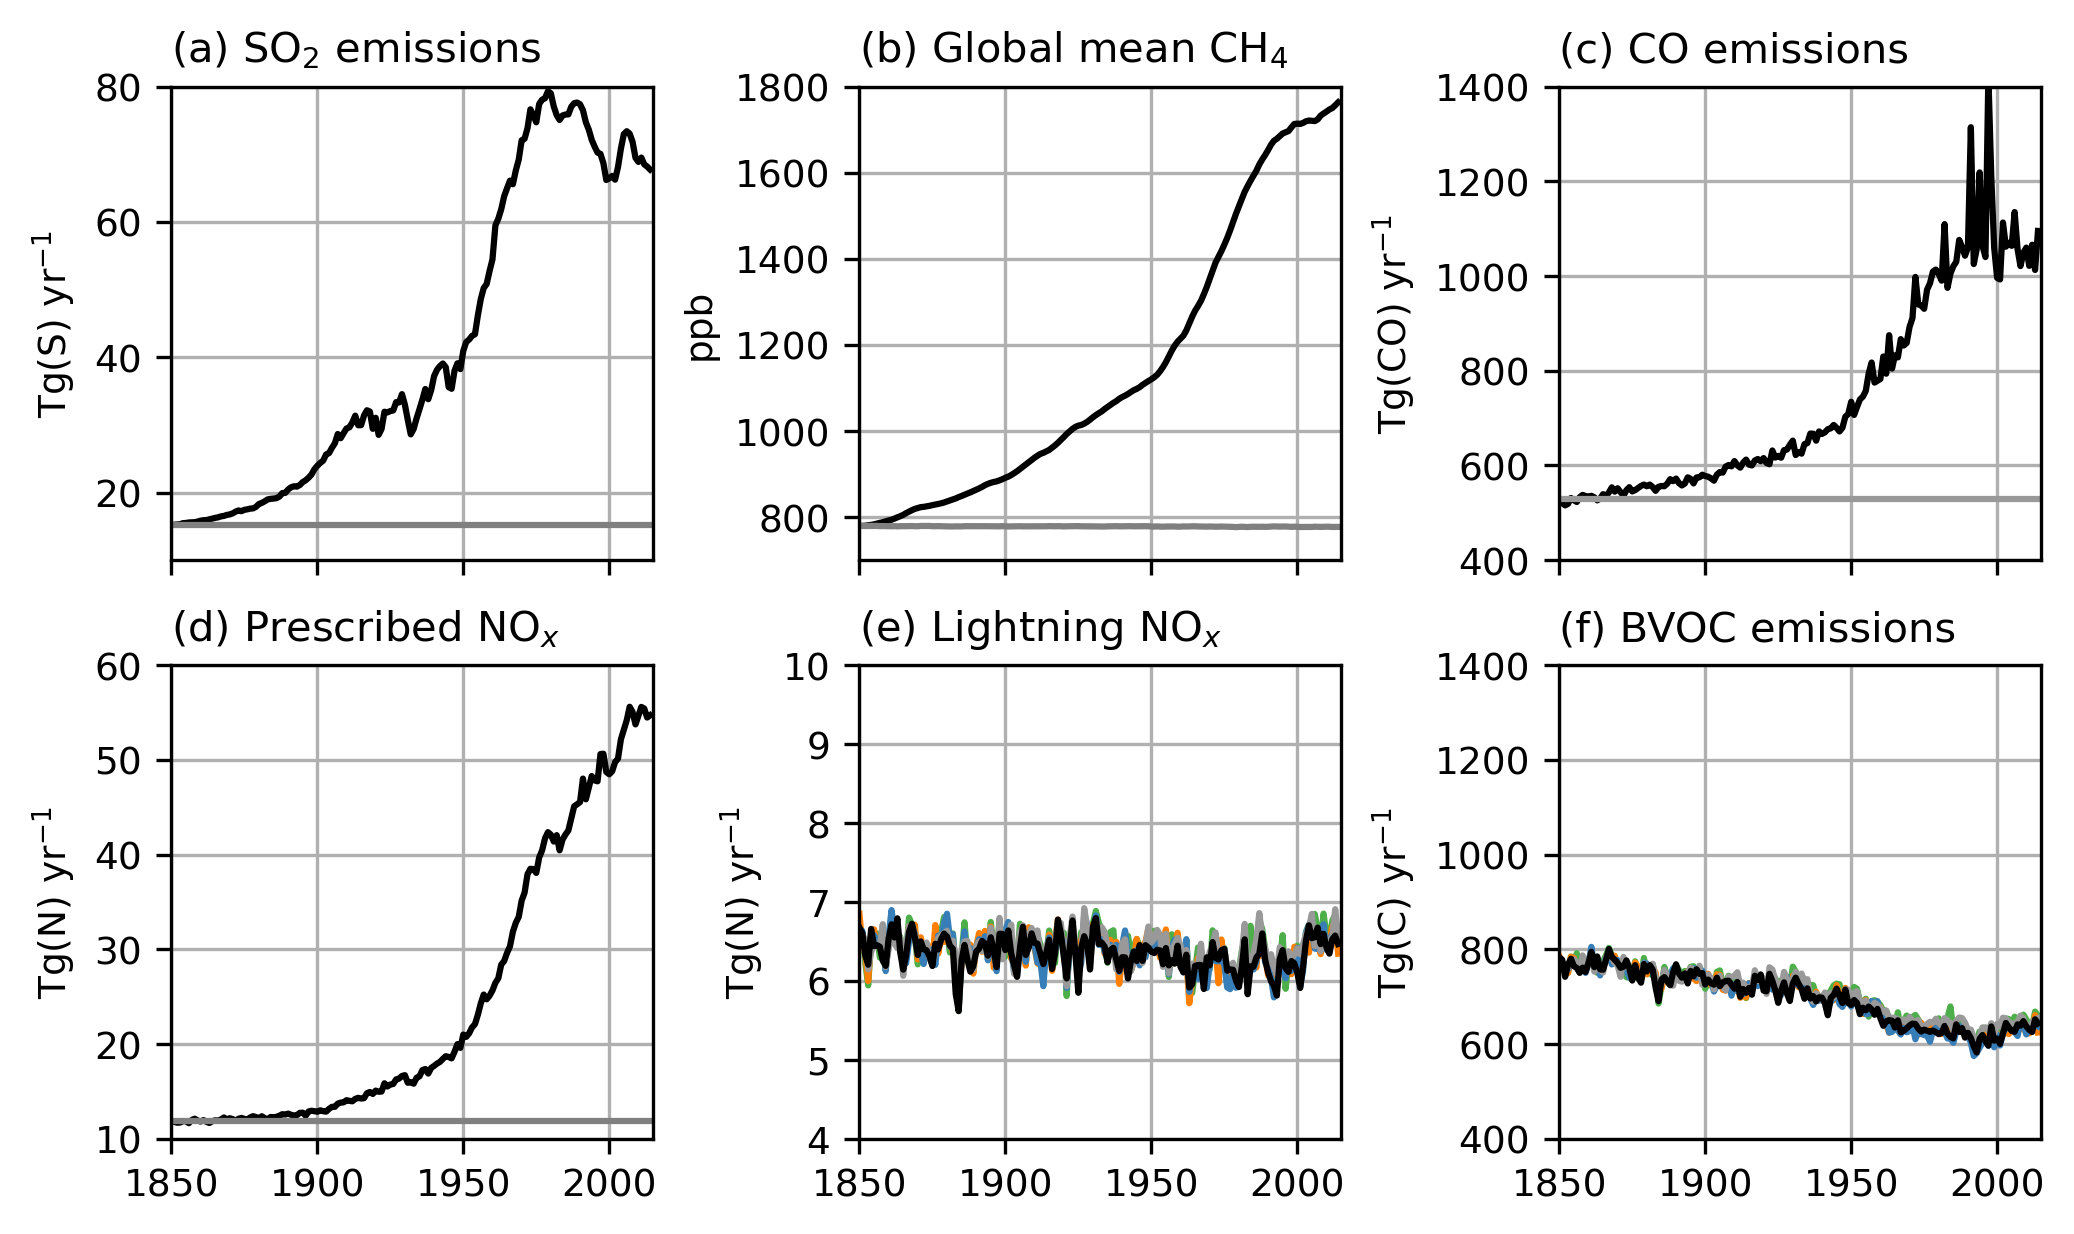
\includegraphics[width=\linewidth]{Chapter3/Figs/f01_emissions.png}
    \caption[Near-term climate forcer emissions and lower boundary conditions used to force AerChemMIP histSST simulations]{Near-term climate forcer emissions and lower boundary conditions used to force simulations listed in Table \ref{tab:ch3:histSST-exp}. (a) Sulfur dioxide emissions include both natural and anthropogenic sources. (b) Methane concentration is constrained at the surface. Emissions of ozone precursors include (c) carbon monoxide, (d) prescribed \ce{NO_x} from surface and aircraft, (e) lightning \ce{NO_x}, and (f) biogenic volatile organic compounds (BVOCs). Lightning  \ce{NO_x} and BVOC are interactively simulated and are shown for each simulation.}
    \label{fig:ch3:emissions}
\end{figure}

In UKESM1, \ce{O3} precursors include surface \ce{NO_x}, lightning \ce{NO_x}, \ce{CO} and biogenic volatile organic compounds (BVOCs) emissions and are calculated from the following CMIP6 variables: \textit{eminox}, \textit{emilnox}, \textit{emico}, and \textit{emibvoc}, respectively. The \textit{eminox} variable is the sum of anthropogenic, biomass burning, soil and aircraft \ce{NO_x}. Biomass burning contributes 6.4 Tg(N) yr$^{-1}$ and soil contributes 5.6 Tg(N) yr$^{-1}$ \citep{archibaldDescriptionEvaluationUKCA2020}. Anthropogenic \ce{NO_x} increases from 0 to 40.2 Tg(N) yr$^{-1}$ between 1850 and 2015. Lighting \ce{NO_x} is simulated interactively in UKESM1 with convective clouds. Historical changes in \ce{NO_x} emissions are driven by changes in anthropogenic \ce{NO_x} at the surface. 
% Isoprene declines - effect on OH and O3, non-linearity in Stevenson 2020.

\ce{CH4} concentration shown in Figure \ref{fig:ch3:emissions} is taken from variable \textit{ch4}. The UKESM1 constrains lower boundary conditions to simulate atmospheric \ce{CH4} concentration. Since \ce{CH4} has a lifetime of 8.1-9.8 years \citep{oconnorAssessmentPreindustrialPresentday2021}, it is well-mixed across the atmosphere from the surface constraint. Figure \ref{fig:ch3:emissions} shows that global \ce{CH4} concentration has increased monotonically since the 1850s from 800 ppb up to 1750 ppb in 2014. 

Aerosol precursors include \ce{SO2}, organic carbons (OCs) and black carbons (BCs). In the UKESM1, sources of BCs are exclusively primary emissions, while sources of OCs are a combination of primary and chemical production of secondary organic aerosol \citep{mulcahyDescriptionEvaluationAerosol2020}. Sulfate aerosols are produced through oxidation. Anthropogenic \ce{SO2} are emitted at the surface, and 2.5\% of the total emission is assumed to be emitted as primary sulfate particles with an aerosol size distribution specified in \citep{stierAerosolclimateModelECHAM5HAM2005}. 

Total \ce{SO2} emissions are calculated from the \textit{emiso2} variable. This includes both primary volcanic and anthropogenic \ce{SO2} emissions but does not include secondary production from DMS oxidation. While anthropogenic \ce{SO2} emissions play a significant role in the overall \ce{SO2} budget, natural emissions are not negligible. However, the AerChemMIP simulations employed in this thesis did not archive the secondary natural \ce{SO2} production from DMS oxidation. Fortunately, secondary production is reported in The UKESM1 18-year AMIP simulation \citep{mulcahyDescriptionEvaluationAerosol2020}. The Atmospheric Model Intercomparison Project (AMIP) is an atmosphere-only configuration for detailed aerosol budget analysis driven by observed sea surface temperature (SST) and sea ice. It reported the emission rate for anthropogenic, primary and secondary natural \ce{SO2} emissions as 60.6, 14.06 and 16.69 Tg(S) yr$^{-1}$, respectively \citep{mulcahyDescriptionEvaluationAerosol2020}. 

\subsection{Research opportunities and motivation}

Compared to its predecessor, HadGEM2-ES, UKESM1 features many enhancement capabilities that allow investigating oxidant perturbations on radiation\citep{sellarUKESM1DescriptionEvaluation2019}. The most notable enhancement is the prognostic aerosol size distribution used by radiation and cloud microphysics, which improves the representation of aerosol radiative forcing. The coupling is both ways, allowing photolytic reaction rates to react to radiative intensity. Oxidation processes for sulfate aerosol are coupled to online chemistry. GLOMAP-mode simulates sulfate aerosol using chemical production from gas and aqueous phases. It also simulates aerosol number and mass concentration independently with inter-modal interactions such as coagulation, condensation, and wet and dry deposition. 

this also us to dig deep into the feedback to aerosol production from changes in other SLCF .


\section{Results and discussions}
\label{sec:ch3:results}



\subsection{Oxidant changes due to near-term climate forcers}

\begin{figure}
    \centering
    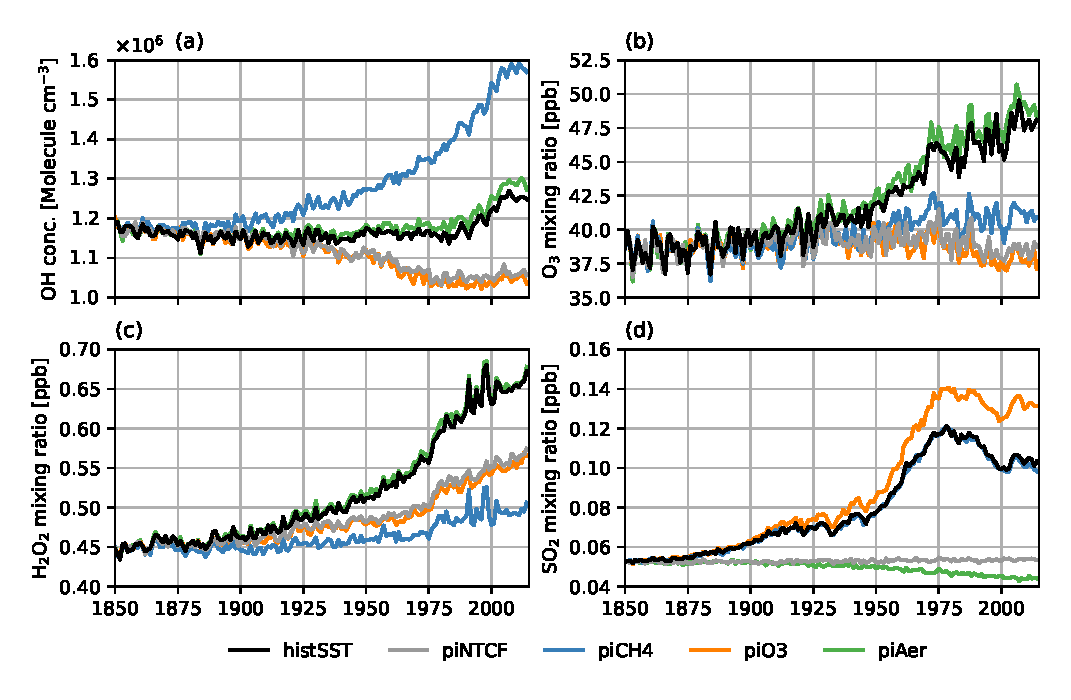
\includegraphics[width=\linewidth]{Chapter3/Figs/f02_oxidant-changes.eps}
    \caption[Global annual mean tropospheric oxidant concentrations or mixing ratios]{Global annual mean tropospheric oxidant concentrations or mixing ratios for species related to \ce{SO2} oxidation in each experiment as mentioned in Table \ref{tab:ch3:histSST-exp}}
    \label{fig:ch3:oxidants}
\end{figure}

Available oxidants play an important role in controlling the oxidation rate. Figure \ref{fig:ch3:oxidants} shows global annual mean of tropospheric oxidants that influence \ce{SO2} oxidation, including \ce{OH}, \ce{O3}, \ce{H2O2} and \ce{SO2}. It shows that the \ce{SO2} mixing ratio follows the \ce{SO2} emission trends (Figure \ref{fig:ch3:emissions}), reaching its peak in 1975 with the maximum mixing ratio reaching 0.14 ppb. \ce{O3} precursor emissions decrease the \ce{SO2} mixing ratio by 27.5\% (from 0.13 to 0.10 ppb) as the decrease in oxidants in the counterfactual, \sstpio{}, decreases the chemical sink of \ce{SO2}. 


Historical \ce{O3} mixing ratio is controlled by \ce{O3} precursor emissions and also \ce{CH4}. Comparing \histsst{} with \sstpio{} in Figure \ref{fig:ch3:oxidants}c, the \ce{O3} mixing ratios show an increase in the historical period with the main source of \ce{O3} coming from \ce{O3} precursors including \ce{NO_x}, \ce{CO} and BVOCs, all of which shows a monotonic increase since 1850 \citep{griffithsTroposphericOzoneCMIP62021}. \ce{CH4} is another source of \ce{O3} as \ce{CH4} forms methyl dioxide (\ce{CH_3O_2}) which reacts with \ce{NO} to form formaldehyde (\ce{HCHO}). \ce{HCHO} photolysis yields \ce{CO} which is a source of tropospheric \ce{O3}. Keeping \ce{CH4} at 1850 level decreases tropospheric \ce{O3} as shown in the Figure \ref{fig:ch3:oxidants}c in \sstpich{}.


Historical \ce{OH} concentrations remain constant until 1975 and increase by \qty{0.1e6}{\per\centi\metre\cubed} by the end of 2014 in the historical trajectory (histSST). The lack of increase in \ce{O3} precursor emissions lowers OH concentration by 15\% (from \num{1.25e6} to \qty{1.05e6}{\per\centi\metre\cubed}) as shown in \sstpio{} and \sstpintcf{} compared to the historical trajectory, \histsst{}. This decrease is due to less OH production by the reaction of water vapour with excited oxygen atoms \ce{(O(^1D))}, which are produced by \ce{O3} photolysis ($\lambda$ < 340 nm). In contrast, for \sstpich{}, where \ce{CH4} concentration is held at the 1850 level, \ce{OH} concentrations increase above the historical trajectory. In this case, OH production rates are lower due to lower \ce{O3} in this simulation. The absence of an increase in \ce{CH4} levels reduces the OH sink via \ce{OH + CH4}. Overall, the effect of historical increases in \ce{CH4} is seen as an increase in OH. The effect of historical increases in \ce{CH4} on OH can be seen since 1875, with the \ce{OH} concentration in 2014 increasing to 133\% that of 1850. 


\ce{H2O2} mixing ratio in the historical period increases after 1850, which could be attributed to NTCF emissions and sea surface temperature (SST). \ce{HO2} produces \ce{H2O2}. Keeping \ce{CH4} at 1850 levels decreases \ce{H2O2} levels as \ce{CH4} is a source of \ce{HO2} radicals, via reactions that form \ce{HCHO} and \ce{HO2} radicals (and hence \ce{H2O2}). \ce{H2O2} is also contributed by \ce{CO}, an \ce{O3} precursor, via its reaction with \ce{OH} to form \ce{HO2}. 


The historical changes of all oxidants are subject to the uncertainty of their sources and chemical processes included in the model. \citet{fanComparisonAnthropogenicEmission2022} reported that \ce{SO2} emissions over China in CMIP6 deviated from the bottom-up, country-level inventory after 2005. This would affect the accuracy of the \ce{SO2} mixing ratio and, consequently, the oxidation downstream. The recent rise in \ce{OH} concentration was also observed in other climate models \citep{zhaoIntermodelComparisonGlobal2019}. 


To summarise this section, historical \ce{O3} precursor emissions promote \ce{OH} concentration, \ce{O3} and \ce{H2O2} mixing ratio. The historical \ce{CH4} reacts away \ce{OH} but boosts \ce{O3} and \ce{H2O2}. The \ce{SO2} emissions from aerosol precursors increase the \ce{SO2} mixing ratio as its main anthropogenic source.

\subsection{\texorpdfstring{\ce{SO2}}{SO2} oxidation and budget changes due to SLCFs}

\subsubsection{\textsoo{} oxidation}
\label{sec:ch3:oxidation}


In the UKESM1, \ce{SO2} reacts with \ce{OH} in the gas phase, forming sulfuric acids which nucleate into sulfate aerosols. \ce{SO2} also reacts and with \ce{H2O2} and \ce{O3} in the aqueous phase to form sulfate aerosols. Figure \ref{fig:ch3:oxidation} shows total annual tropospheric \ce{SO2} oxidation tendencies in each pathway. In the historical period, \ce{SO2} oxidation by \ce{OH} is the largest of the three pathways, contributing 20 Tg(S) yr$^{-1}$ globally in 2014. The \ce{SO2 + OH} trend broadly follows the \ce{SO2} emissions and the \ce{OH} concentration trends. The lower \ce{OH} concentration decreases \ce{SO2 + OH} reaction tendencies in \sstpio{}, and, similarly, the increase in OH concentration in \textit{piCH4} enhances \ce{SO2 + OH} reaction tendencies.

\begin{figure}
    \centering
    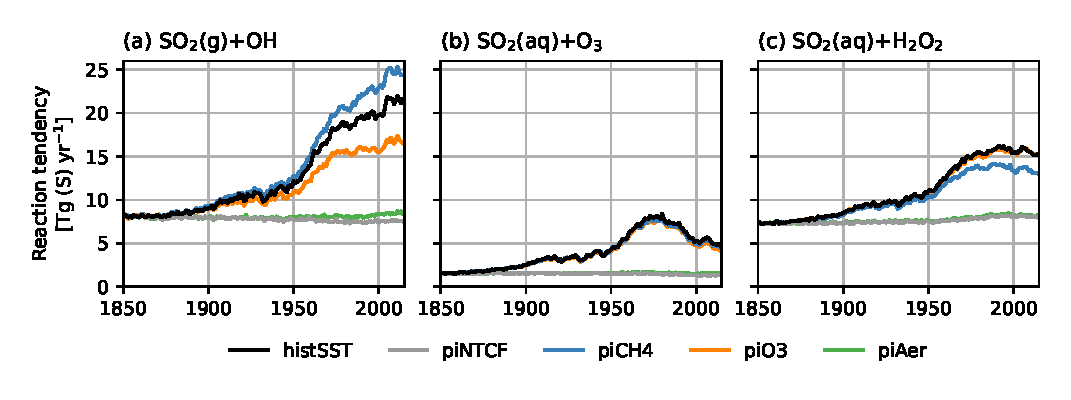
\includegraphics[width=\linewidth]{Chapter3/Figs/f03_oxidation.eps}
    \caption[Global annual \ce{SO2} oxidation tendencies]{Global annual \ce{SO2} oxidation tendencies between 1850-2014 with changes due to constraining  methane concentration (\textit{piCH4}), aerosol precursors (\sstpiaer{}), ozone precursors (\sstpio{}) or both emissions (\textit{piNTCF}) at 1850 level.}
    \label{fig:ch3:oxidation}
\end{figure}


\ce{SO2 + O3} reaction tendencies, however, are not sensitive to changes in \ce{O3} mixing ratios. Figure \ref{fig:ch3:oxidants}b shows that the global \ce{O3} mixing ratio monotonically increases after 1850, but historical \ce{SO2 + O3} does not share the trend. As a result of anthropogenic \ce{O3} precursor emissions being fixed at the 1850 level in \sstpio{}, the \ce{O3} concentration is lower than that of \textit{histSST}. Despite the 25\% decrease in \ce{O3} mixing ratio in \sstpio{} and \textit{piCH4}, there are minimal changes to \ce{SO2 - O3} tendencies in these experiments compared to \textit{histSST}. The lack of change implies that globally \ce{SO2 + O3} oxidation is not sensitive to historical changes in \ce{O3} and that the background tropospheric \ce{O3} is sufficient to saturate the pathway. 

\ce{SO2 + H2O2} oxidation tendencies follow the \ce{SO2} emissions and \ce{H2O2} mixing ratio trends. The historical oxidation tendency starts at 7.5 Tg(S) yr$^{-1}$ and increases to 16 Tg(S) yr$^{-1}$ and stabilises after the 1980s. The \ce{SO2 + H2O2} reaction tendencies decrease by 15\% when the \ce{H2O2} mixing ratio decreases in the absence of anthropogenic \ce{CH4} which is a source of \ce{H2O2} precursor. 


While past measurements and laboratory research have determined that only \ce{OH} is important for the oxidation of \ce{SO2} in the gas phase during daytime \citep[][and reference therein]{rattiganUptakeGasphaseSO22000, eatoughConversionSO2Sulfate1994}, heterogeneous and aqueous-phase oxidation is more complex with multiple competing oxidants and aerosol properties at play \citep{pattantyusReviewSulfurDioxide2018, seinfeldAtmosphericChemistryPhysics2016}. 

Other \ce{SO2} oxidation pathways may be important in certain environments such as clean marine boundary layers and wintertime. The oxidation of S(IV) in the atmosphere includes organic peroxides, and iron and manganese as catalysts to oxygen \citet{alexanderTransitionMetalcatalyzedOxidation2009, seinfeldAtmosphericChemistryPhysics2016}. A further mechanism for \ce{SO2} oxidation in solution with sea water is proposed via halogen compounds \ce{HOCl} and \ce{HOBr} in the remote marine boundary layer \citep{vogtMechanismHalogenRelease1996}. Aside from oxidation with \ce{OH}, \ce{O3} and \ce{H2O2}, these further mechanisms are not included in the UKESM1 so they are not considered in this study. 


%discuss change to oxidation if ph is changed in Tunnock


Overall, the rate of \ce{SO2} oxidation with \ce{OH}, \ce{O3} and \ce{H2O2} is controlled by \ce{SO2} abundance, as the reaction tendency tends to be constant over time without aerosol precursor emissions (green line in Figure \ref{fig:ch3:oxidation}). The \ce{OH} and \ce{H2O2} pathways contribute equally to \ce{SO2} oxidation in the 1850s but the rate of growth of \ce{SO2 + OH} oxidation is greater post-1950s, making \ce{SO2 + OH} the most important oxidising pathway. \ce{O3} is the least important oxidant globally, contributing to the removal of at most 8 Tg(S) yr$^{-1}$. Overall, the \ce{SO2 + OH} pathway is the most sensitive to oxidant changes in which the spread between \sstpio{} and \textit{piCH4} is approximately 5 Tg(S) yr$^{-1}$ or 25\% of the \textit{histSST} oxidation rate in 2014.



\subsubsection{\texorpdfstring{\ce{SO2}}{SO2} and \texorpdfstring{\ce{SO4}}{SO4} burdens, losses, lifetimes, and budgets}

\begin{figure}
    \centering
    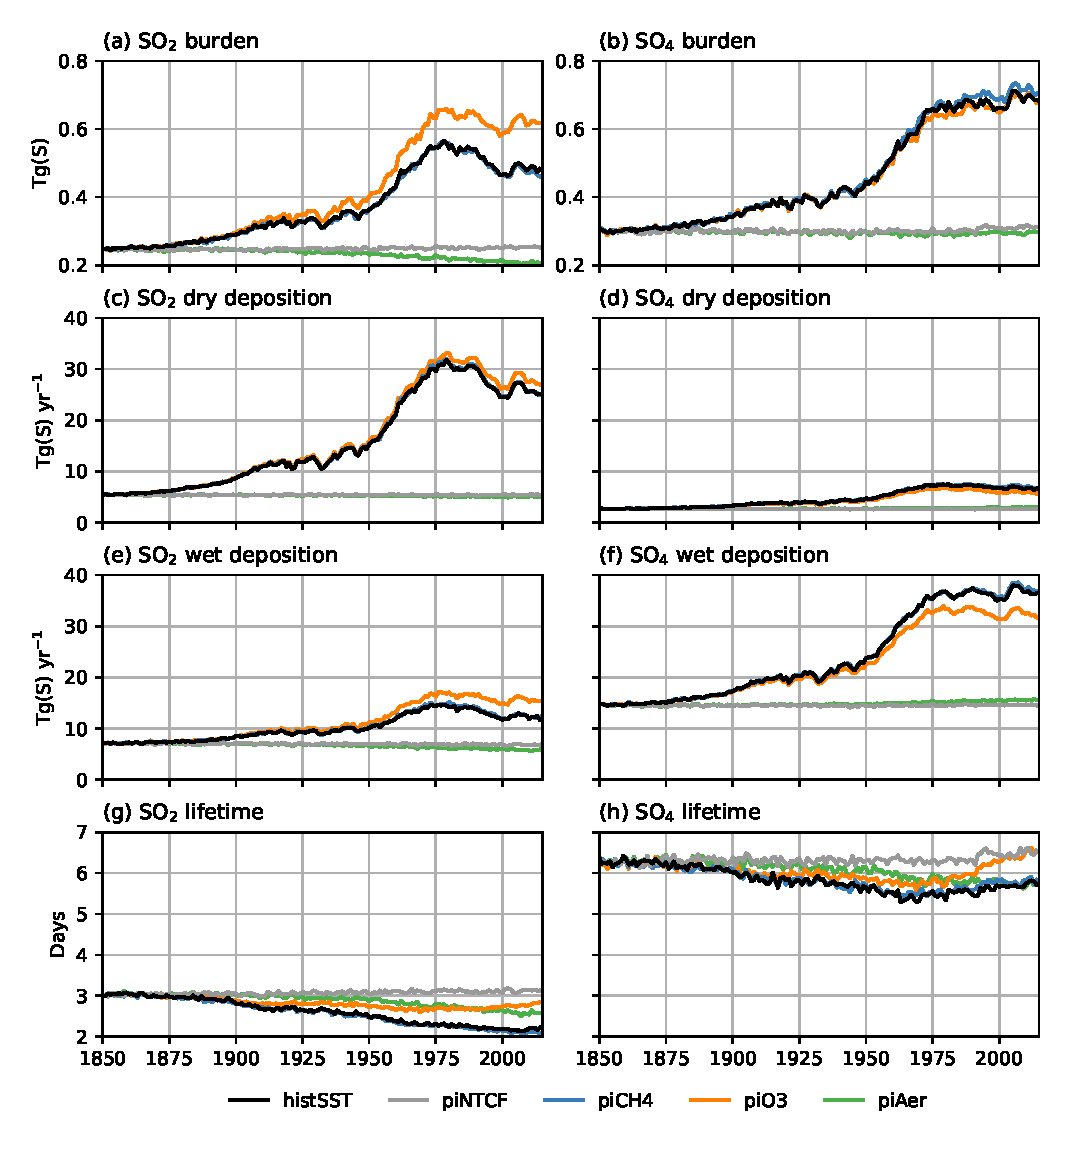
\includegraphics[width=\linewidth]{Chapter3/Figs/f04_s-budget.eps}
    \caption[Tropospheric sulfur budget: burdens, depositions and lifetimes]{Tropospheric \ce{SO2} and \ce{SO4} budget, including (a-b) burdens, (c-d) dry depositions, (e-f) wet depositions, and (g-h) lifetimes. The plots show budget terms between 1850-2014 with changes due to constraining  methane concentration (\textit{piCH4}), aerosol precursors (\sstpiaer{}), ozone precursors (\sstpio{}) or both emissions (\textit{piNTCF}) at the 1850 level.}
    \label{fig:ch3:s-burden}
\end{figure}

\ce{SO2} reacts with \ce{OH}, \ce{H2O2} and \ce{O3} to form sulfate (\ce{SO4}) so the budget of \ce{SO2} and \ce{SO4} are linked via these oxidation processes. Figure \ref{fig:ch3:s-burden} shows that the \ce{SO2} burden trend follows that of \ce{SO2} emissions. \ce{SO2} is lost mainly through oxidation (45 Tg(S) yr$^{-1}$ in 2014) followed by dry deposition (28 Tg(S) yr$^{-1}$). The lifetime of \ce{SO2} is 3 days in the 1850s and decreases to 2.8 days in 2014. 

Oxidants affect the \ce{SO2} budget in various ways. The lifetime of a trace gas describes how long it stays in the atmosphere and is defined as the average time that a molecule of that species remains in a reservoir before removal. Suppose the reservoir is the whole atmosphere and is in a steady state. In that case, the burden is considered constant, and the tropospheric lifetime of a compound is estimated by dividing the total tropospheric burden by total loss. \ce{SO2} loss terms include chemical losses via oxidation with \ce{OH}, \ce{O3}, and \ce{H2O2}, wet and dry deposition. \ce{SO4} is lost only via wet and dry deposition.

The lower levels of \ce{O3} in \sstpio{} result in less \ce{OH}, which leads to a smaller \ce{SO2} sink than in \textit{histSST}. This increases the \ce{SO2} burden, dry and wet deposition and ultimately leads to a longer lifetime. This change to the \ce{SO2} budget due to lower \ce{O3} is also seen in \sstpiaer{} and \textit{piNTCF} where \ce{SO2} is kept at the 1850 level throughout the historical period. In \textit{piNTCF}, in which \ce{O3} precursor emissions are kept at the 1850 level (low \ce{O3}), the \ce{SO2} burden, wet and dry deposition and lifetime are lower compared to the case that \ce{O3} precursors follow the historical trajectory (\sstpiaer{}). This further indicates the role of \ce{O3} in the \ce{SO2} budget via oxidation with \ce{OH}.


In contrast to \sstpio{}, where the lower \ce{O3} and oxidant levels increase \ce{SO2}, the \ce{SO2} burden stays roughly the same when \ce{CH4} concentration is kept at 1850 level in \textit{piCH4}, despite the huge differences in \ce{CH4} and as a result OH (see Figure \ref{fig:ch3:emissions}). This is because whilst there is a significant increase in \ce{SO2 + OH} oxidation in \textit{piCH4}, this is nullified by the decrease in \ce{SO2 + H2O2} oxidation as seen in figure \ref{fig:ch3:oxidation}a and c. In this case, the \ce{SO2} lifetime remains unchanged compared with the \textit{histSST}.

Figure \ref{fig:ch3:s-burden} shows that, in \sstpio{}, exposing \ce{SO2} emissions to pre-industrial \ce{O3} increases the lifetime of both \ce{SO2} and \ce{SO4}. The effect of oxidant changes to \ce{SO2} lifetime was observed in a modelled study by \citep{karsetStrongImpactsAerosol2018}. They found that by replacing oxidants (\ce{NO3}, \ce{O3}, \ce{OH} and \ce{HO2}) from present-day to pre-industrial, the lifetime of pre-industrial \ce{SO2} increases from 29 hours (1.21 days) to 34 hours (1.42 days), which is an increase by 17\%. In this work, the \ce{SO2} lifetime increases by 28\% (from 2.17 days to 2.77 days). As aerosols have a longer lifetime, they are transported higher up in the atmosphere before oxidising, making them less likely to be removed by deposition. The dry deposition of the newly formed nucleation mode \ce{SO4} decreased by 2.6\%. 

The \ce{SO4} burden is generally higher than that of \ce{SO2} because of its longer lifetime. The \ce{SO4} burden has increased from 0.3 to 0.7 Tg(S) yr$^{-1}$ between 1850 and 2014. Because UKESM1 treats \ce{SO4} as an aqueous aerosol, the primary removal process for \ce{SO4} is wet deposition. The lifetime of \ce{SO4} is 5.5-6 days, double that of \ce{SO2}. Changes in oxidants have a knock-on effect on \ce{SO4} budget and lifetime. In \sstpio{} where anthropogenic \ce{O3} is missing, there is less \ce{SO4} wet deposition as there is less conversion from \ce{SO2} to \ce{SO4} and more physical removal of \ce{SO2} (via both wet and dry deposition). This reduction in \ce{O3} and oxidants in \sstpio{} also results in an increase in \ce{SO4} lifetime compared to \textit{histSST}. 


The budget report in our work is comparable to that reported by the UKESM1 evaluation using AMIP simulation covering 1981-1998 \citep{mulcahyDescriptionEvaluationAerosol2020}. The AMIP \ce{SO2} and \ce{SO4} are 0.53 and 0.67 Tg(S), respectively, the same as our values. For dry deposition, the AMIP values for \ce{SO2} and \ce{SO4} are 28.98 and 7.10 Tg(S) yr$^{-1}$, comparable to that of ours of 28.90 and 7.13 Tg(S) yr$^{-1}$. As for the wet deposition, the AMIP reported 13.38 and 36.0 Tg(S) yr$^{-1}$ for \ce{SO2} and \ce{SO4}, while our results are 13.47 and 36.40 Tg(S) yr$^{-1}$. Finally, the AMIP lifetime of \ce{SO2} and \ce{SO4} are 2.08 and 5.56 days, respectively, which are comparable to our work (2.23 and 5.56 days).  

The SLCFs simulated by UKESM1 have been evaluated against both ground-based measurements and field campaigns \citep[e.g.][]{griffithsTroposphericOzoneCMIP62021, russoSeasonalInterannualDecadal2023}. The UKESM1 CMIP6 simulations capture the \ce{SO4} trends compared to ground-based measurements \citep{mulcahyDescriptionEvaluationAerosol2020}. The observed decreasing trend in \ce{SO4} concentration across Europe is reproduced by the model. Although there is a consistent underprediction of the absolute values for all years, the model prediction sits within the observed variability. The UKESM1 overestimated \ce{SO2} concentration compared to the Atmospheric Tomography (ATom) field campaign which measures atmospheric constituents and chemical processes in marine remote areas across both hemispheres \citep{ranjithkumarConstraintsGlobalAerosol2021}. The UKESM1 model overestimated \ce{SO2} concentration by approximately a factor 2–6 in the boundary layer regions of the tropics and mid-latitudes and the tropical upper troposphere. The biases in the upper-tropospheric mid and high latitudes are negligible. This may imply that the \ce{SO2} removal process is underestimated or that the natural secondary emissions from DMS are overestimated.  

An in-depth evaluation has shown that the UKESM1 underestimated the dry deposition process and there has been an update released for the model to amend for this error \citep{hardacreEvaluationSO2SO422021}. Model evaluation against ground-based measurements shows that while the UKESM1 captures historical trends for decreasing the concentration of \ce{SO2} and \ce{SO4}, it overpredicts \ce{SO2} by a factor of 3 and underpredicted surface \ce{SO4} by 25-35\% \citep{hardacreEvaluationSO2SO422021}. This has led to an update to the UKESM1 configuration called the UKESM1.1 \citep{mulcahyUKESM11DevelopmentEvaluation2023}. When a more realistic dry deposition scheme is implemented, it reduces the model’s overprediction of surface \ce{SO2} concentrations and total column \ce{SO2} but also decreases the overall \ce{SO4} loading, exacerbating the low bias.  Our study used the original UKESM1 thus the overestimation of \ce{SO2} is expected.


\subsection{Aerosol properties changes due to SLCFs}

\subsubsection{Aerosol optical depth}

\begin{figure}
    \centering
    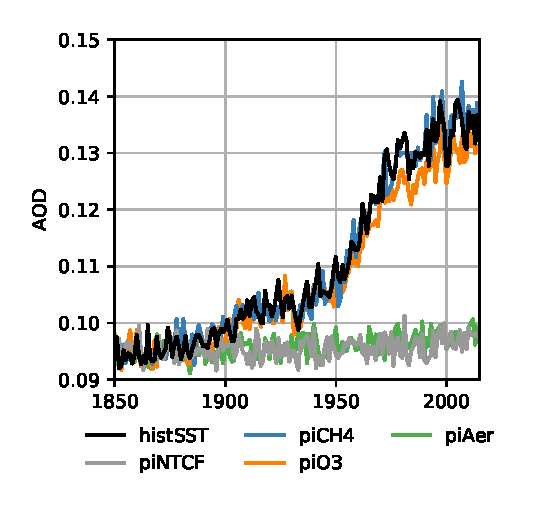
\includegraphics{Chapter3/Figs/f05_aod-trend.eps}
    \caption[Global annual mean aerosol AOD between 1850-2014 with changes due to SLCFs]{Global annual mean aerosol AOD between 1850-2014 with changes due to constraining methane concentration (\textit{piCH4}), aerosol precursors (\sstpiaer{}), ozone precursors (\sstpio{}) or both emissions (\textit{piNTCF}) at 1850 level.}
    \label{fig:ch3:AOD}
\end{figure}


The amount of aerosol in the atmosphere is linked to \ce{SO2} oxidation tendency as it produces \ce{SO4} aerosols. Figure \ref{fig:ch3:AOD} shows annual global mean AOD from different experiments. It shows that aerosol precursors increase AOD by 50\% and are the main contributor to global AOD. AOD in the piO3 experiment is lower than histSST by 0.05, suggesting that ozone contributes to some aerosol formation. Global AOD is unchanged under lower \ce{CH4} condition in piCH4.

\begin{figure}
    \centering
    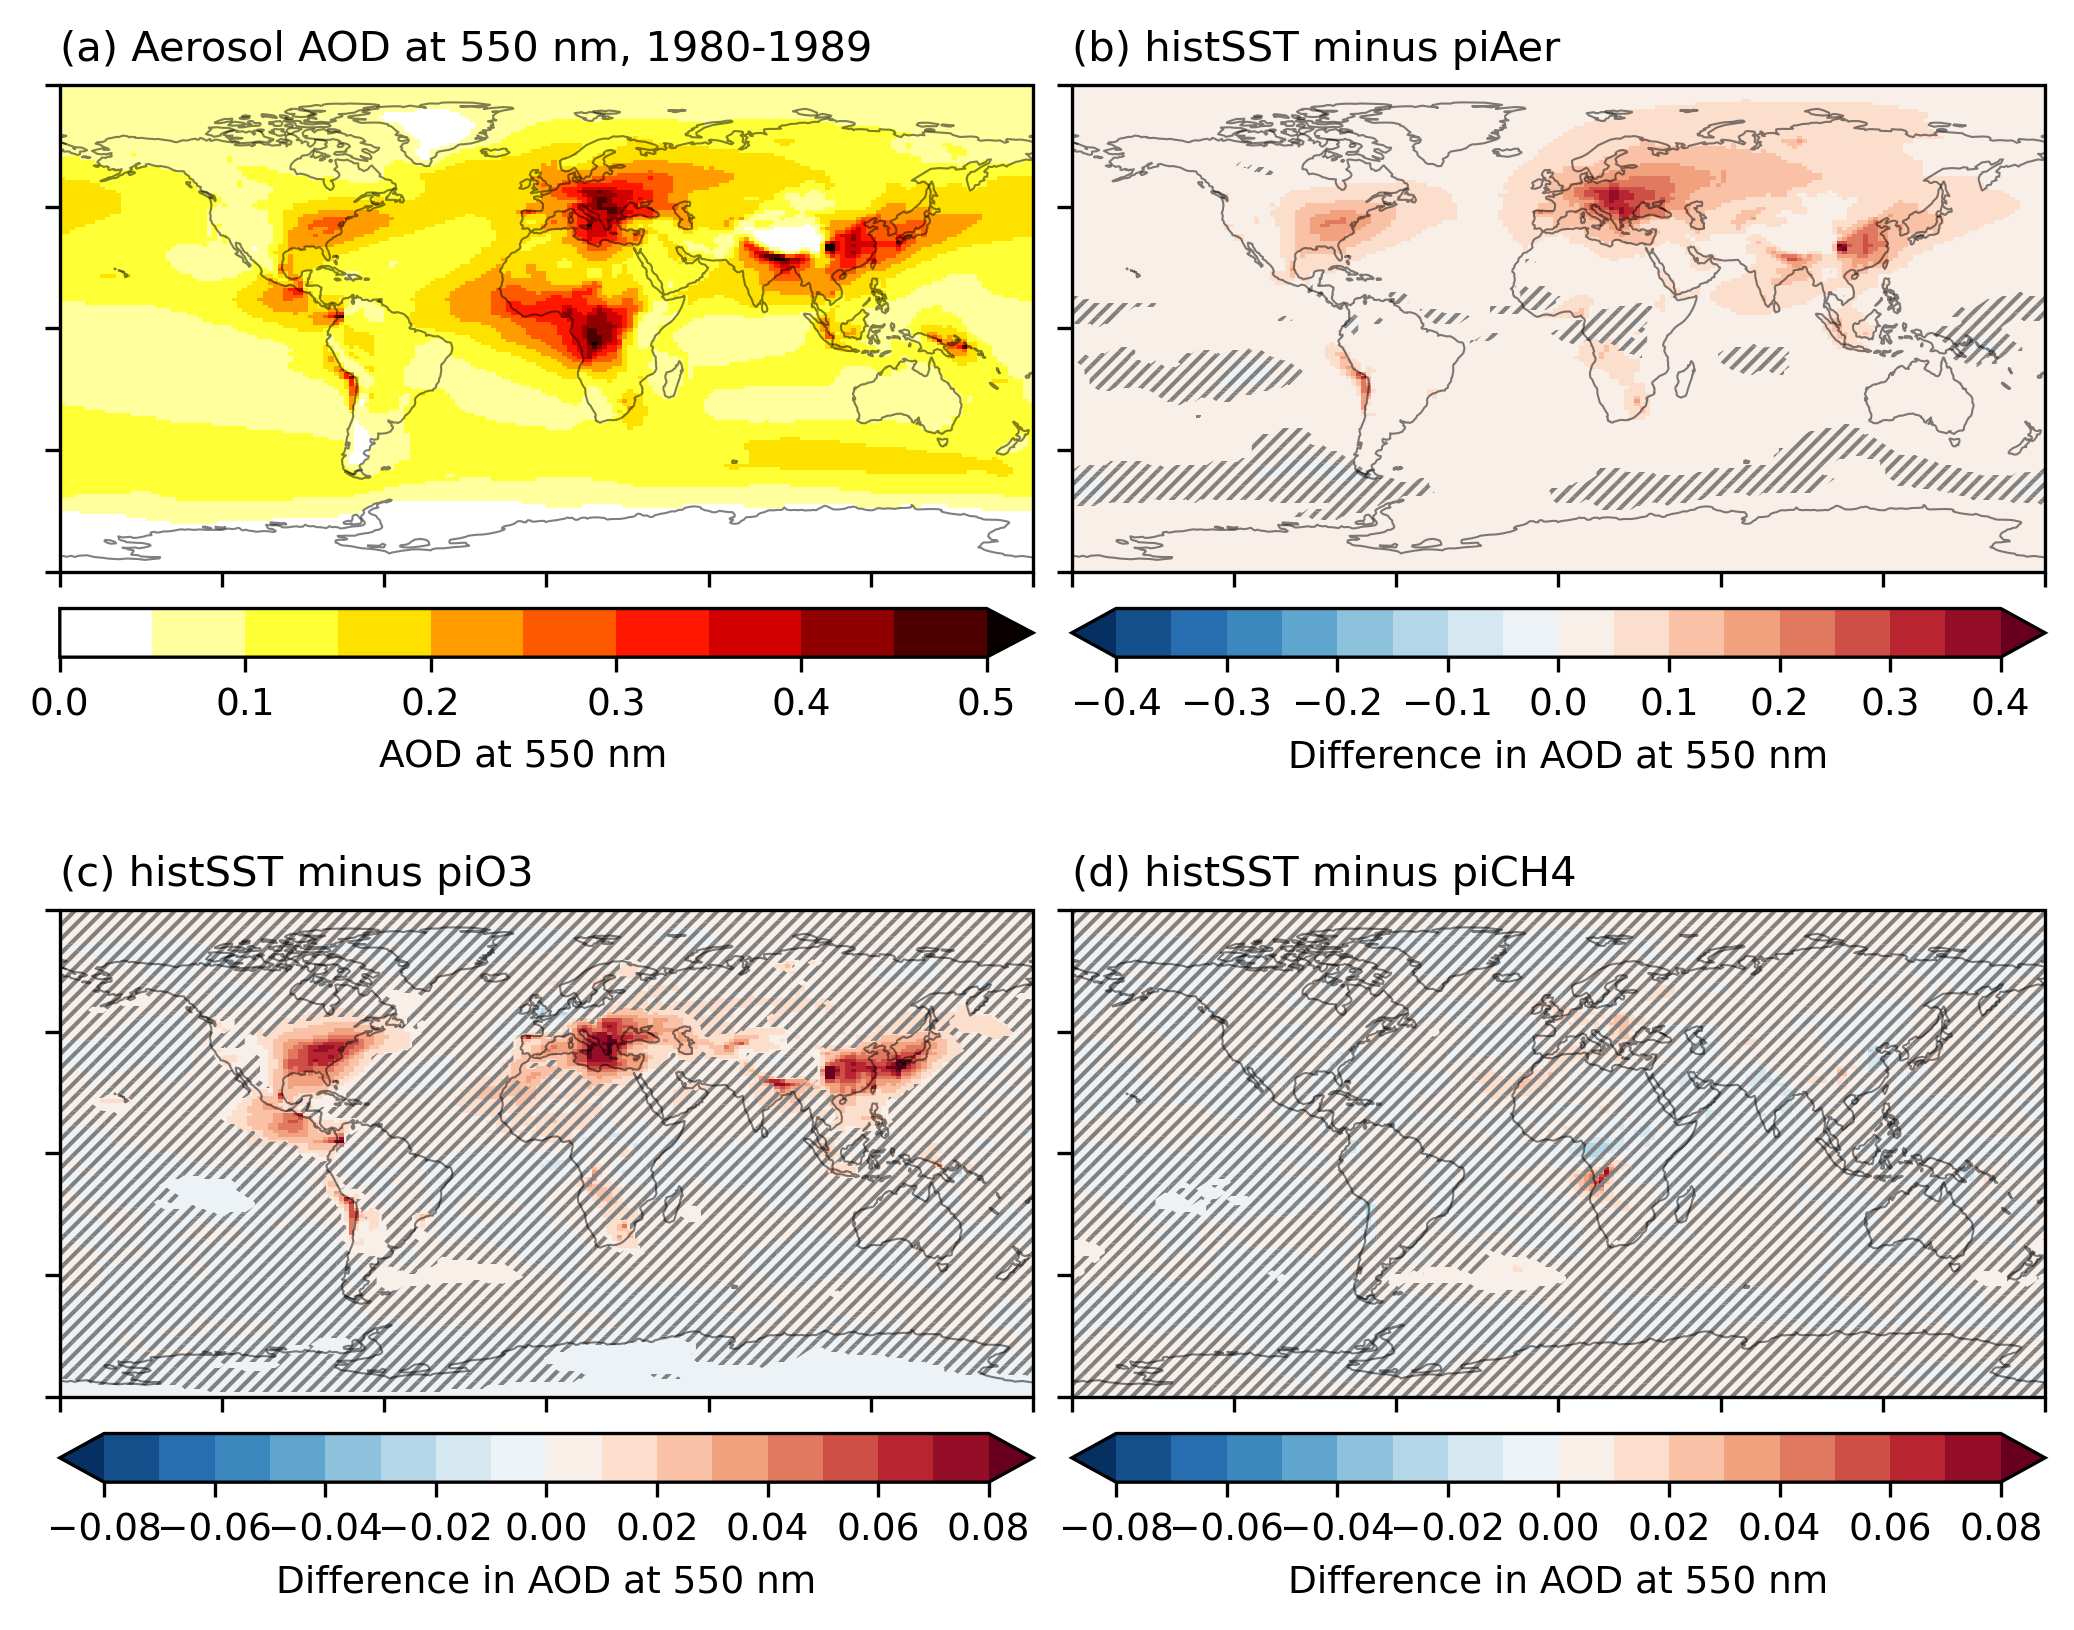
\includegraphics[width=\linewidth]{Chapter3/Figs/f06_aod-map.png}
    \caption[Mean aerosol AOD at 550 nm from 1980-1989 and changes to AOD due to SLCFs]{(a) Decadal mean aerosol AOD at 550 nm from 1980-1989. (b-d) Difference of aerosol AOD at 550 nm from 1980-1989 between \textit{histSST} and \sstpiaer{}, \sstpio{}, and \textit{piCH4}, respectively. Hatched areas denote areas in which the difference is not statically significant (p$\leq$0.05)}
    \label{fig:ch3:AOD-map}
\end{figure}


Figure \ref{fig:ch3:AOD-map} shows the location of AOD changes due to oxidants. There is a localised increase of AOD in the high emission areas such as Northern America, Central Europe, and Eastern Asia due to aerosol precursor emissions in the 1980s, when the main aerosol precursor is \ce{SO2}. \ce{O3} precursors are responsible for 20\% of AOD in these areas (0.08 out of 0.4 over the European region, for example). \ce{CH4} has an insignificant effect on AOD. This is due to the nullifying nature of the change: increase of \ce{SO2 + OH} oxidation and the decrease in \ce{SO2 + H2O2} which results in approximately net zero change in total oxidation tendency compared to \textit{histSST}. This shows that although a global change of reaction tendency was observed, it may not be reflected in some aerosol diagnostics such as AOD. We note here that anthropogenic \ce{CH4} is shown, in the next section, to affect cloud properties.

% Compare the AOD evaluation in Mulcahy and also discuss the updated AOD from Hardarcre and UKESM1.1
AOD simulated by the UKESM1 against both ground-based measurements and satellite retrievals and found good agreement in trends but underestimated the absolute values \citep{mulcahyDescriptionEvaluationAerosol2020}. The global annual mean AOD trends from AMIP simulation between 1980-2015 show an overall increase in AOD which is consistent with the Collection 6 MODIS merged dataset (MODIS C6) satellite retrieval. The absolute AOD is underestimated by 0.03 but is still within the lower end of the range of the satellite AOD. The spatial distribution shows that the UIKESM1 has higher AOD in the winter seasons of each hemisphere. This is due to the high sea-salt emission which peaks in the winter months. The high bias in sea-salt AOD does not affect our analysis which subtracts AOD from \sstpiaer{}, \sstpio{} and \textit{piCH4} with \textit{histSST}.

% discuss the updated effect of dry deposition from UKESM1 with UKESM1.1
The UKESM1 was updated with a new dry deposition scheme and a revised dust tuning which affects the predicted aerosol AOD \citep{mulcahyUKESM11DevelopmentEvaluation2023}. The new version of UKESM1, the UKESM1.1, predicted a lower aerosol AOD, with a difference of at least 0.02 starting from 1980 due to a higher \ce{SO2} dry deposition which removes \ce{SO2} from the atmosphere, leaving less to oxidise to form \ce{SO4}. This new dry deposition scheme further increases the low bias in \ce{SO4} concentration compared to measurements. The annual mean AOD from UKESM1 and UKESM1.1 over 2003-2014 shows that the global mean AOD predicted by the models are 0.137 and 0.146, respectively, which are lower than most satellite measurements from MODIS (0.162), ORAC (0.170) and Swansea (0.135). These products, their uncertainties and details of the evaluation procedure are described in detail in \citet{mulcahyDescriptionEvaluationAerosol2020}. The spatial increase in the AOD in UKESM1.1 stems from the revised dust tuning which increases the dust AOD over and downwind of major dust source regions. This update is not relevant to \ce{SO2} oxidation. However, there is a decrease in AOD in UKESM1.1 over China due to an increase in \ce{SO2} dry deposition. Our work used output from the original UKESM1 thus the AOD will have a less low bias in absolute AOD and higher overall \ce{SO4} loading.



\subsubsection{Aerosol size distribution}
\label{sec:ch3:result:aerosol-size-dist}

\begin{figure}
    \centering
    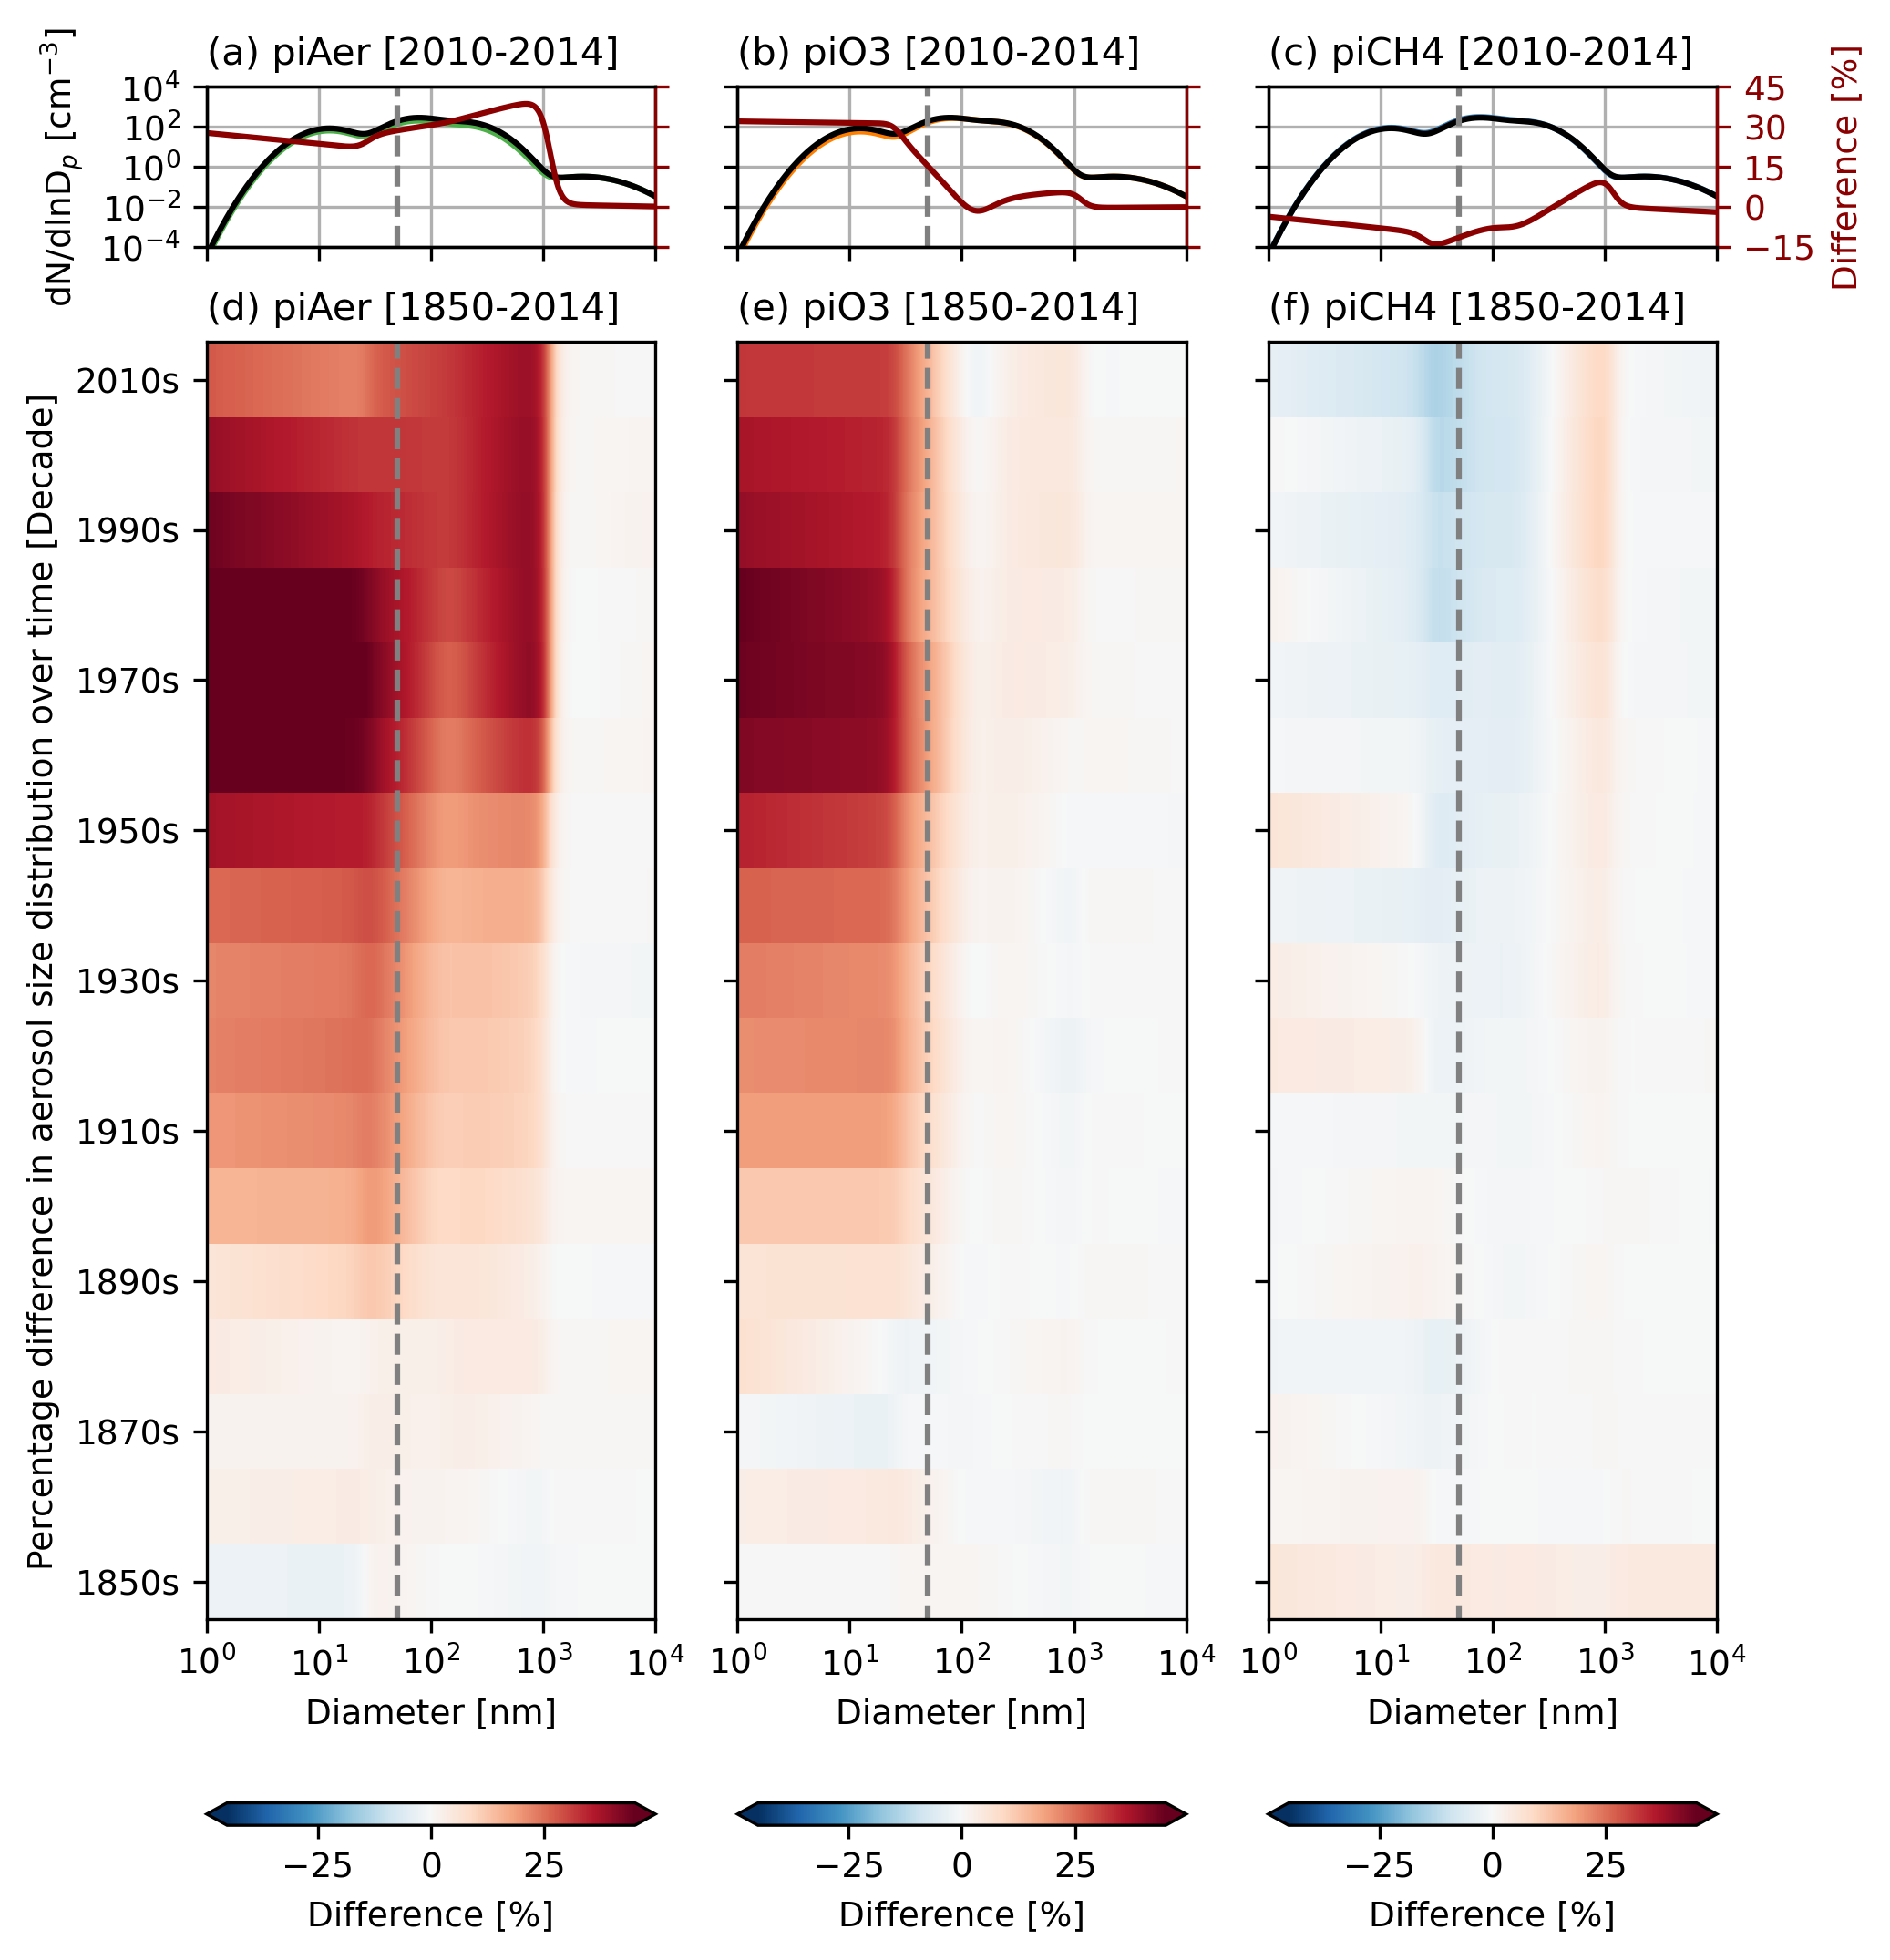
\includegraphics[width=\linewidth]{Chapter3/Figs/f08_aerosol-size-dist-over-time.png}
    \caption[Aerosol size distribution for 2010-2014 at 1 km]{(top) Historical total aerosol size distribution at 1 km for 2010-2014 with percentage difference on the secondary axis. (bottom) The progression of percentage change of aerosol size distribution due to (d) aerosol precursors, (e) \ce{O3} precursors, and (f) \ce{CH4}. The vertical dashed line denotes the 50 nm diameter (25 nm radius) above which aerosol affects cloud nucleation.}
    \label{fig:ch3:aerosol-size-dist-time}
\end{figure}


Perturbation to oxidants modifies global aerosol size distribution over the historical period. The top panels of figure \ref{fig:ch3:aerosol-size-dist-time} show aerosol size distribution and percentage differences between \textit{histSST} and the \sstpiaer{}, \sstpio{} and \textit{piCH4} simulations for 2010-2014 at 1 km. The bottom panels show the progression of change in aerosol size over time. In panels (d - f), each horizontal bar denotes the percentage difference of global decadal mean aerosol size distribution at 1 km between \textit{histSST} and the perturbed simulations. For example, the percentage differences for 2010-2014 in figures (a-c) are plotted as the topmost colour bar in figures (d-f). 

As shown by figure \ref{fig:ch3:aerosol-size-dist-time}d, historical aerosol precursor emissions increase aerosol concentrations with diameters smaller than 50 nm by more than 40\%  between the 1960s and 1980s. The number of particles greater than 50 nm in diameter (N50 -- dashed grey vertical line) has increased by 30-35\% and this is likely to affect the concentration of cloud condensation nuclei (CCN) \citep{seinfeldAtmosphericChemistryPhysics2016}. In contrast, historical \ce{O3} precursors increase the concentration of particles with a diameter of less than 50 nm by 30\% but only increase the concentration of particles with a diameter above 50 nm by 4\%. As shown in Section \ref{sec:ch3:oxidation}, the \ce{O3} precursors affect only the \ce{SO2 + OH} reaction tendency which forms new sulfate aerosol particles. The \textit{piCH4} shows that the historical increase in \ce{CH4} leads to an increase in the aerosol concentration with a diameter above 1000 nm by 8\% after the 1970s; however, the concentration of aerosol at this size is negligible, with only 1-2 particles per cm${^3}$. More importantly, an increase in \ce{CH4} concentration decreases the aerosol concentration up to 300 nm diameter as the increase in \ce{CH4} decreases the \ce{SO2 + OH} reaction tendency which contributes to new aerosol formation. 

% add discussions on the results by O'Connor
This result agrees with other work which reported a change in aerosol size distribution due to \ce{CH4} \citep{oconnorApportionmentPreIndustrial2022}. They found that an increase in \ce{CH4} concentration in the present day leads to a significant reduction in aerosol number concentration in Aitken and accumulation mode. The reduction in N50 occurs across all latitudes and through the depths of the atmosphere. As \citet{oconnorApportionmentPreIndustrial2022} used timeslice simulations in their work, this work adds to their finding that the reduction in N50 occurs as early as the 1920s and increases in magnitude over time, to a maximum relative difference of 15\% in 2010. 

\subsection{Cloud properties}

\begin{figure}
    \centering
    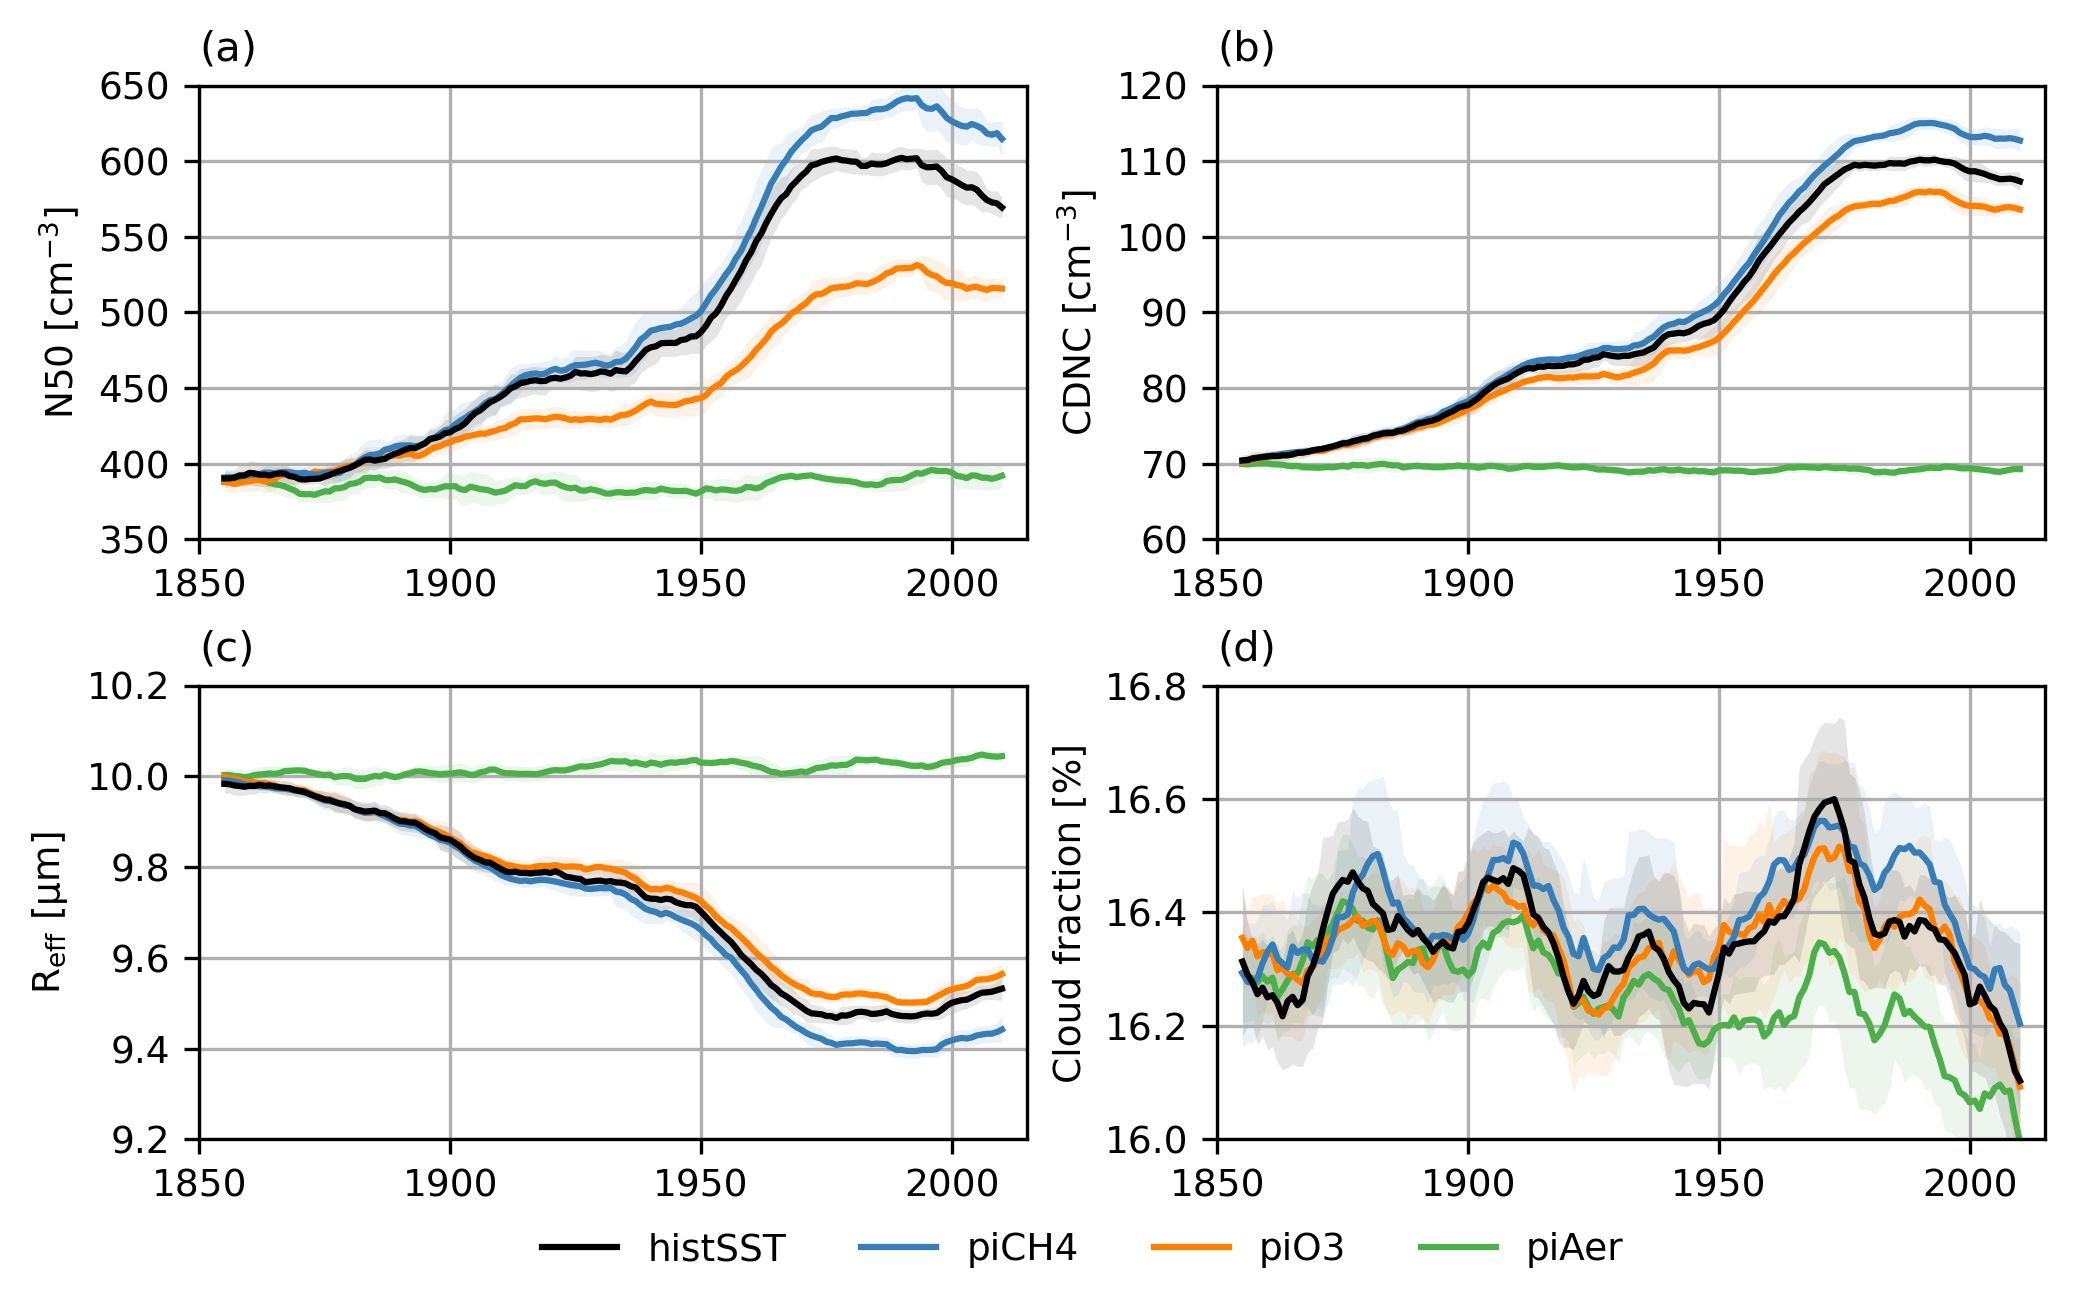
\includegraphics[width=\linewidth]{Chapter3/Figs/f09_cloud-props.png}
    \caption{Change in annual mean (a) concentration of particles greater than 50 nm diameter (N50), (b) cloud droplet number concentration (CDNC), (c) effective cloud droplet radius (R$_{\textrm{eff}}$) and (d) cloud fraction at 1 km. A 10-year rolling mean was applied to the data. Shaded areas denote the standard deviation from the 10-year mean.}
    \label{fig:ch3:cloud}
\end{figure}

Aerosols with a diameter above 50 nm (N50) act as cloud condensation nuclei (CCN) in which their concentration modifies cloud properties. Figure \ref{fig:ch3:cloud} shows the global decadal mean N50 concentration as well as cloud properties including cloud droplet number concentration (CDNC), cloud droplet effective radius (R$_{\textrm{eff}}$) and cloud fraction at 1 km. It shows that N50 rises from 400 cm$^{-3}$ in 1850 to 600 cm$^{-3}$ in the 1980s then decreases slightly in the historical period. This trend is in line with cloud properties change. \ce{O3} precursors are responsible for 12.5\% (75 cm$^{-3}$  of 600 cm$^{-3}$) of total N50 in 1980s. Meanwhile, an increase in N50 in \textit{piCH4} implies that historical anthropogenic methane emissions lower N50 concentration.

Cloud properties show signs of changes due to aerosol precursors and oxidant changes. Figure \ref{fig:ch3:cloud}b shows global mean cloud properties at 1 km above ground. CDNC increases by 40 cm$^{-3}$ due to aerosol precursors. Historical \ce{O3} precursors increase CDNC while \ce{CH4} decreases CDNC. This is linked to the change in \ce{SO2 + OH} reaction tendency as this reaction increases aerosol number in the atmosphere, which will affect CDNC \citep{twomeyInfluencePollutionShortwave1977}. While AOD, seen in figure \ref{fig:ch3:AOD-map}, does not indicate a significant change due to \ce{CH4}, cloud properties show a clear increase to CDNC and a decrease to R$_{\textrm{eff}}$. This is in line with work done by \citet{karsetStrongImpactsAerosol2018}, which found that the distribution of the changes in aerosol number concentration does not always correspond directly to the distribution of the changes in cloud and radiative properties. In essence, historical \ce{CH4} increases the cloud effective radius and decreases CDNC.

Cloud fraction increases by 0.2\% due to aerosol precursors. However, \ce{O3} and \ce{CH4} do not significantly alter cloud fractions as shown in \ref{fig:ch3:cloud}c. 


\subsection{Radiative effects due to SLCFs}

Greenhouse gases, aerosols, and clouds could perturb the Earth's radiative balance. One way to quantify the effect of each of the forcings is through the decomposition of effective radiative forcing (ERF) as described in Section \ref{sec:ch2:erf}. The ERF is decomposed into the clear and clean sky part or $ERF_{cs,clean}$, the instantaneous radiative forcing of the aerosol (ie, scattering and absorption) or aerosol IRF, and the cloud radiative effect or $\Delta$CRE'. Here we show that \ce{O3} precursors affect aerosol IRF and that \ce{CH4} affects the cloud radiative effect.

\begin{figure}
    \centering
    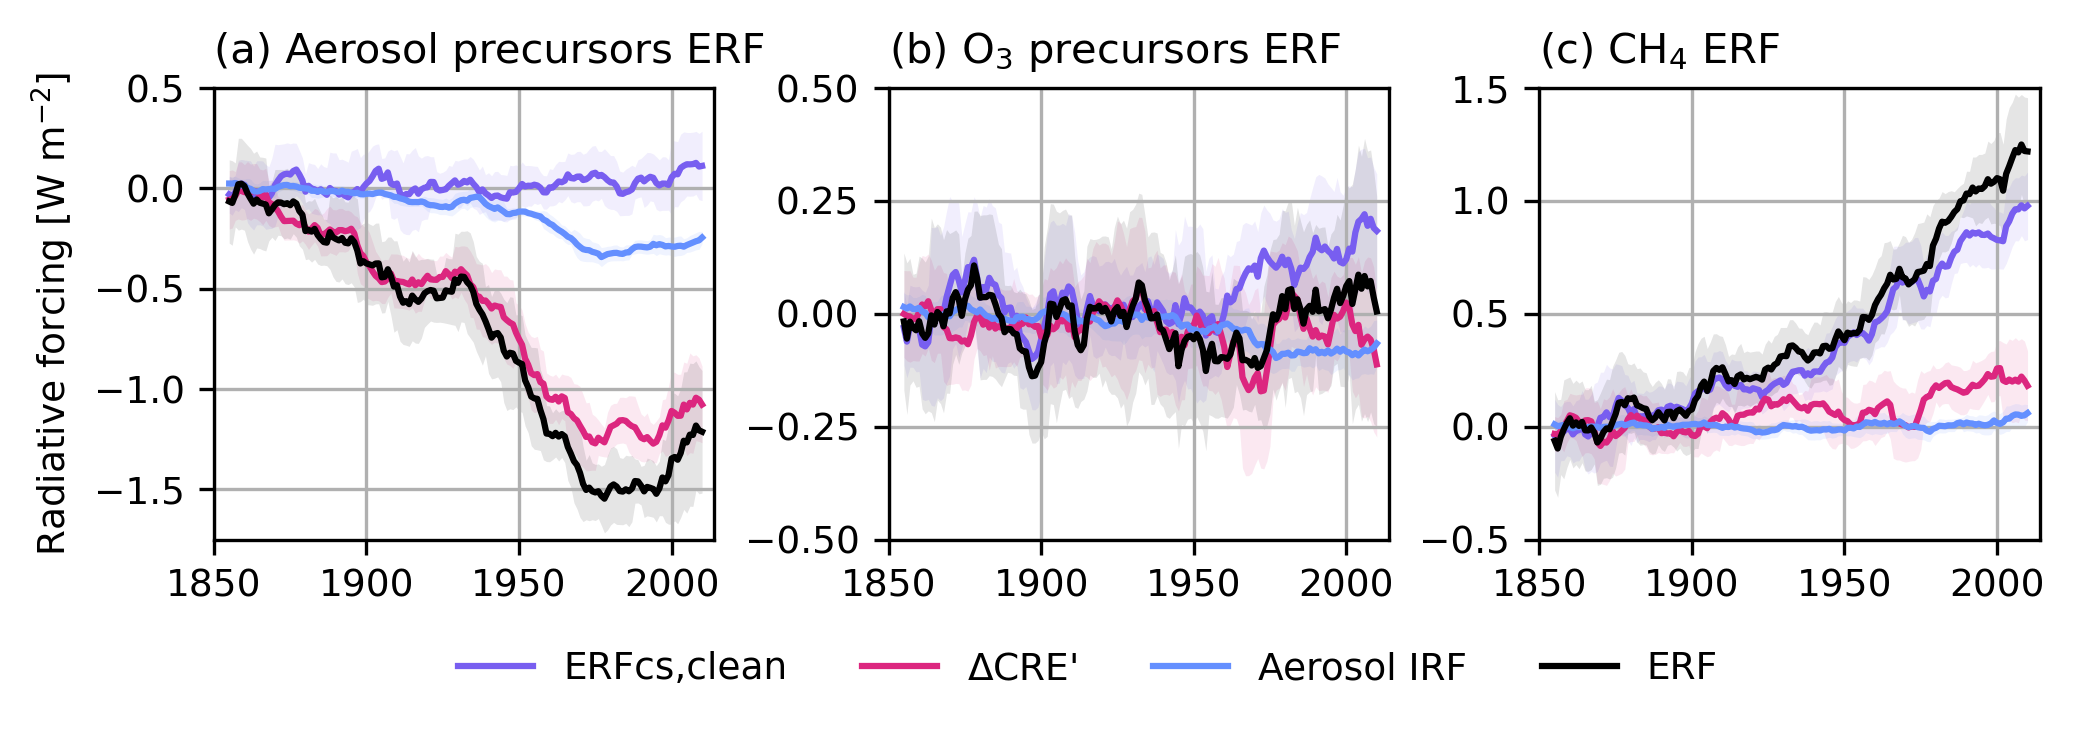
\includegraphics[width=\linewidth]{Chapter3/Figs/f10_erf.png}
    \caption[Global mean radiative forcing due to SLCFs]{Global mean aerosol radiative forcing due to (a) aerosol precursors, (b) \ce{O3} precursors and (c) \ce{CH4}. A 10-year rolling mean was applied to the data. Shaded areas denote the standard deviation from the 10-year mean.}
    \label{fig:ch3:erf}
\end{figure}
% sstpiaer
% irf -0.2772347016768022
% irf_std 0.031058704
% cre -1.0905492262406782
% cre_std 0.19105731
% sstpio3
% irf -0.08279982263391668
% irf_std 0.05211312
% cre -0.04306954470547763
% cre_std 0.16057429
% sstpich4
% irf 0.039096790010278874
% irf_std 0.037890494
% cre 0.21275067762895067
% cre_std 0.15470749

Figure \ref{fig:ch3:erf} shows the global annual mean aerosol ERF from aerosol precursors, \ce{O3} precursors and \ce{CH4}. Figure \ref{fig:ch3:erf}a shows that aerosol precursors contribute mostly to the cloud radiative effects (-1.01$\pm$0.19 W m$^{-2}$), followed by aerosol IRF (-0.18$\pm$0.04 W m$^{-2}$). Aerosol precursor ERF is the most negative between 1970-1990 due to an increase in both cloud radiative effect and instantaneous radiative forcing. Aerosol precursors include absorbing aerosols such as black carbons which contribute to net positive IRF in some regions such as eastern central China \citep{seoImpactsAerosolEmissions2020, oconnorAssessmentPreindustrialPresentday2021}. 


\ce{O3} is an important greenhouse gas \citep{forsterEarthEnergyBudget2021}. By itself, the present-day change in \ce{O3} has a positive (warming) clear-sky radiative forcing of 0.25 W m$^{-2}$ compared to 1850. There is a slight decrease in aerosol IRF due to \ce{O3} precursors starting in the 1960s and up to 0.08$\pm$0.05 W m$^{-2}$ between 2000-2014. This is due to the increase in new aerosol formation from the \ce{SO2 + OH} reaction tendency since the amount of scattered solar radiation is proportional to the total column mass burden of particles \citep{nemesureDirectShortwaveForcing1995}. As seen in Figure \ref{fig:ch3:AOD-map}, there is a statistically significant change to AOD due to \ce{O3} precursors. There is no clear change to cloud radiative effects due to \ce{O3}, consistent with \citet{skeieHistoricalTotalOzone2020}, who reported that cloud adjustments due to \ce{O3} are in the order of 0.02 W m$^{-2}$. However, we note that the UKESM1 is the only model with troposphere and stratosphere chemistry that gives negative ERF in the present-day \citet{skeieHistoricalTotalOzone2020}. 

\ce{CH4} is a greenhouse gas that also affects the cloud adjustment \citep{oconnorApportionmentPreIndustrial2022}. The increase in \ce{CH4} in the present-day has resulted in an increase in the clear-sky radiative forcing of 1.0 W m$^{-2}$ since 1850. Changes in \ce{CH4} since 1850 have resulted in negligible changes in the aerosol direct effect. This is due to the reaction tendency of \ce{SO2 + OH} and \ce{SO2 + H2O2} roughly cancelling out, resulting in an unchanged aerosol loading as shown in the aerosol AOD, figure \ref{fig:ch3:AOD-map}. On the other hand, the decrease to CDNC and increase in cloud droplet effective radius from 1850s to historical \ce{CH4} results in a positive cloud radiative effect of 0.21$\pm$0.15 W m$^{-2}$. These results agree with the time slice study reported in \citep{oconnorApportionmentPreIndustrial2022}.

% discuss oconnor in details
\citet{oconnorApportionmentPreIndustrial2022} showed that the increase in \ce{CH4} concentration leads to changes to aerosol properties, which leads to a positive total \ce{CH4} ERF. Their study used two timeslice experiments: pre-industrial and pre-industrial with present-day \ce{CH4} to calculate the aerosol ERF. The ERF estimates suggest that the total \ce{CH4} ERF from UKESM1 includes a significant indirect contribution from aerosols. The direct CH4 ERF at the present-day relative to the preindustrial period is 0.85$\pm$0.03 W m$^{-2}$ \citep{oconnorAssessmentPreindustrialPresentday2021}.

% Discuss Thornhill 2021 (Multi model Aerosol ERF calculation from different NTCF including CH4 and O3 - See Table 5)



\section{Conclusions}

Changes in oxidants due to \ce{O3} precursors and \ce{CH4} affect sulfate aerosol formation, cloud formation and potentially radiative balance, but the impacts of oxidants on ERF are not well understood. In this work, we used results from AerChemMIP experiments to investigate the effects of oxidant changes on sulfate aerosol formation, aerosol and cloud properties and aerosol effective radiative forcing. We have explained the relationship between a net negative change to IRF by \ce{O3} and a net positive change by \ce{CH4} to CRE to changes in oxidation due to respective forcers.  

% Effects due to O3
Historical \ce{O3} precursor emissions increase \ce{O3} mixing ratio as well as \ce{OH} and \ce{H2O2}. These oxidant increases enhance the \ce{SO2 + OH} reaction tendency and significantly increase the aerosol AOD near high \ce{SO2} emission regions.  Due to \ce{O3} precursors, the concentration of aerosols with size below 50 nm increases, which increases the cloud droplet number concentration but does not result in significant changes in cloud radiative effects. Ultimately, ozone precursors increase the aerosol instantaneous radiative forcing by up to 0.08$\pm$0.05 W m$^{-2}$ between 2000-2014, which is 44\% of aerosol IRF due to aerosol precursors, further cooling the climate.

% Effects due to CH4
On the other hand, \ce{CH4} decreases the OH concentration as \ce{CH4} acts as an OH sink. Increases in \ce{CH4} also increases \ce{H2O2} and \ce{O3} mixing ratios. These changes in oxidants decrease the OH reaction tendency (\ce{SO2 + OH}) but increase the \ce{SO2 + H2O2} reaction tendency, resulting in an unchanged sulfate budget but a larger mean aerosol diameter as the \ce{H2O2} oxidation occurs in the liquid phase where aerosol growth occurs more easily. This change in aerosol size distribution minimises CDNC and enhances the effective cloud droplet radius. As a result,\ce{CH4} contributes to a positive cloud radiative effect of 0.21$\pm$0.15 W m$^{-2}$ between 2000-2014, further adding to the warming impact of methane on the climate.

Changes in aerosol precursor emissions have had an important impact on the climate offsetting a significant fraction of the warming from long-lived greenhouse gases \citep{szopaShortlivedClimateForcers2021}. However, we have shown here that accounting for oxidants over the historical period is important to accurately simulate sulfate aerosol formation and the resulting aerosol radiative effects. Up to 40\% of the change in aerosol direct radiative may be the result if ERF is calculated using oxidant from the present day.  

%%!TEX root = ../thesis.tex

\chapter{An analysis of the seasonal cycle of aerosol radiative forcing in UKESM1}
\label{ch4:title}

\section*{Abstract}

Sulfate aerosol modelling in Earth System Models (ESMs) has advanced from early 1-dimensional models in the 1980s to the interactive, prognostic aerosol components in CMIP6 models. Despite these advancements, recent CMIP6 models underperformed relative to lower-complexity models in predicting surface air temperatures during the 1960-–1990 period, a phenomenon known as "pothole cooling". This discrepancy has been linked to sulfate aerosol loading, but no clear relationship has been found between pothole cooling and aerosol sensitivity. Additionally, the chapter reviews the seasonal variation of sulfur dioxide (\ce{SO2}) oxidation, with studies indicating more gas-phase oxidation and stronger radiative effects in summer due to increased photochemical activity. However, a comprehensive analysis of these seasonal trends in CMIP6 models, including the role of Earth system processes in models like UKESM1, remains lacking. This chapter aims to investigate the variation in aerosol cooling driven by seasonal changes in aerosol precursors and to assess whether summertime aerosol-radiation effects contribute to pothole cooling. 

Using the UK Earth System Model 1 (UKESM1), this chapter investigates sulfate aerosol formation under emissions and oxidant changes between 1850 and 2014. Simulation outputs from the Aerosol Chemistry Model Intercomparison Project (AerChemMIP) are analysed. The results show that emission timing determines oxidation tendency via the available oxidant and meteorological properties such as clouds. In UKESM1, \ce{SO2} reacts with OH in the gas phase and \ce{O3} and \ce{H2O2} in the aqueous phase. Up to 80\% of total sulfate production is via gas phase oxidation in boreal summer when high OH and low cloud cover are observed. The opposite is true for wintertime when aqueous phase reactions with \ce{O3} and \ce{H2O2} form up to 90\% of aerosol. This work shows that effective radiative forcing per unit of \ce{SO2} emissions in summer is four times greater than that of winter during the pothole period. An analysis of these monthly changes of oxidants and emissions to sulfur oxidation, aerosol and cloud properties and connect these to effective radiative forcing are presented. Finally, surface air temperature changes are presented for the pothole cooling period. 


\section{Introduction}
\label{ch4:intro}

Sulfate aerosol modelling in the ESMs has advanced since the 1980s when it started as 1-dimension model with prescribed meteorology and chemical fields \citep[e.g. ][]{ericksoniiiGlobalOceantoatmosphereDimethyl1990} \change{add more refs}. In the latest climate  model intercomparison project (CMIP6), many ESMs features interactive chemical solvers and prognostic aerosols \citep{zhangRoleAnthropogenicAerosols2021}. However, when pitched against observations, these sophisticated models performed worse in predicting surface air temperature between 1960—1990, known as the pothole cooling or anomalous cooling, compared to lower-complexity models \citep{zhangRoleAnthropogenicAerosols2021}. Research on aerosol radiative effects uses aerosol sensitivity as a proxy for measuring model cooling caused by aerosol and used this to compare different models. However, it has been shown that pothole cooling correlates with sulfate loading while showing no relationship between pothole cooling and aerosol sensitivity \citep{zhangRoleAnthropogenicAerosols2021}.

Another vein of sulfate aerosol modelling explores the seasonality of \ce{SO2} oxidation and radiative effect. Observations from downwind of coal-fired factories has looked at the seasonal trend of \ce{SO2} oxidation and documented the seasonal variation of oxidation  \citep{meagherSeasonalVariationAtmospheric1983}. This has been confirmed by modelling study, showing that there is indeed more gas-phase oxidation during summer when there is more photochemical reactions producing OH \citep{meagherSeasonalVariationAtmospheric1983,eatoughConversionSO2Sulfate1994}\change{more refs}.

Four ESMs from the CMIP5 agree that \ce{SO2} emitted during summer has more potential to cause negative radiative forcing \citep{bellouinRegionalSeasonalRadiative2016}. These models are either ctm or gcm. Only 2 GCM has interactive tropospheric ozone chemistry, one of which is the HadGEM3, the predecessor to UKESM1. These two models shows large discrepancies between radiative forcing between summer and winter. 

However, a comprehensive analysis of this phenomena for CMIP6 models is not yet explored. In particular, the additional Earth system processes included in UKESM1 will lead to fundamental differences in aerosol sources, evolution and sinks. Whether the pothole cooling and summertime enhanced aerosol-radiation effect are related has not been investigated. This chapter attempts to address: a)  the variation in aerosol cooling caused by aerosol precursor in different season and the mechanism underpinning the process, in an attempt to b) understand whether summer cooling could explain pothole cooling.


\subsection{Anomalous cooling in surface air temperature in CMIP6 models}
\label{ch4:sec:pothole}

Earth system models have grown more complex with increasing interactions and coupling over time to represent the Earth as accurate as possible. This enables researchers to study the earth system is a way that has not been possible decades ago. With more processes and interaction between systems, the models are expected to be able to simulate the Earth system more accurately; however; this has not always been the case for surface air temperature in many of the CMIP6 models \citep{zhangRoleAnthropogenicAerosols2021}. 

All models that participate in CMIP6 are required to provide \hist{} simulation which could be used to compare the model against each other and with observation \citep{eyringOverviewCoupledModel2016}. Six ESMs with interactive chemistry that participated in the CMIP6 and AerChemMIP, including UKESM1, exhibited a low bias in surface air temperature compared to observation \citep{zhangRoleAnthropogenicAerosols2021}. The anomalous cooling is the period between 1960 and 1989 inclusive when ESMs consistently underpredict the surface air temperature compared to observation \citep{zhangRoleAnthropogenicAerosols2021}. 

\begin{figure}
    \centering
    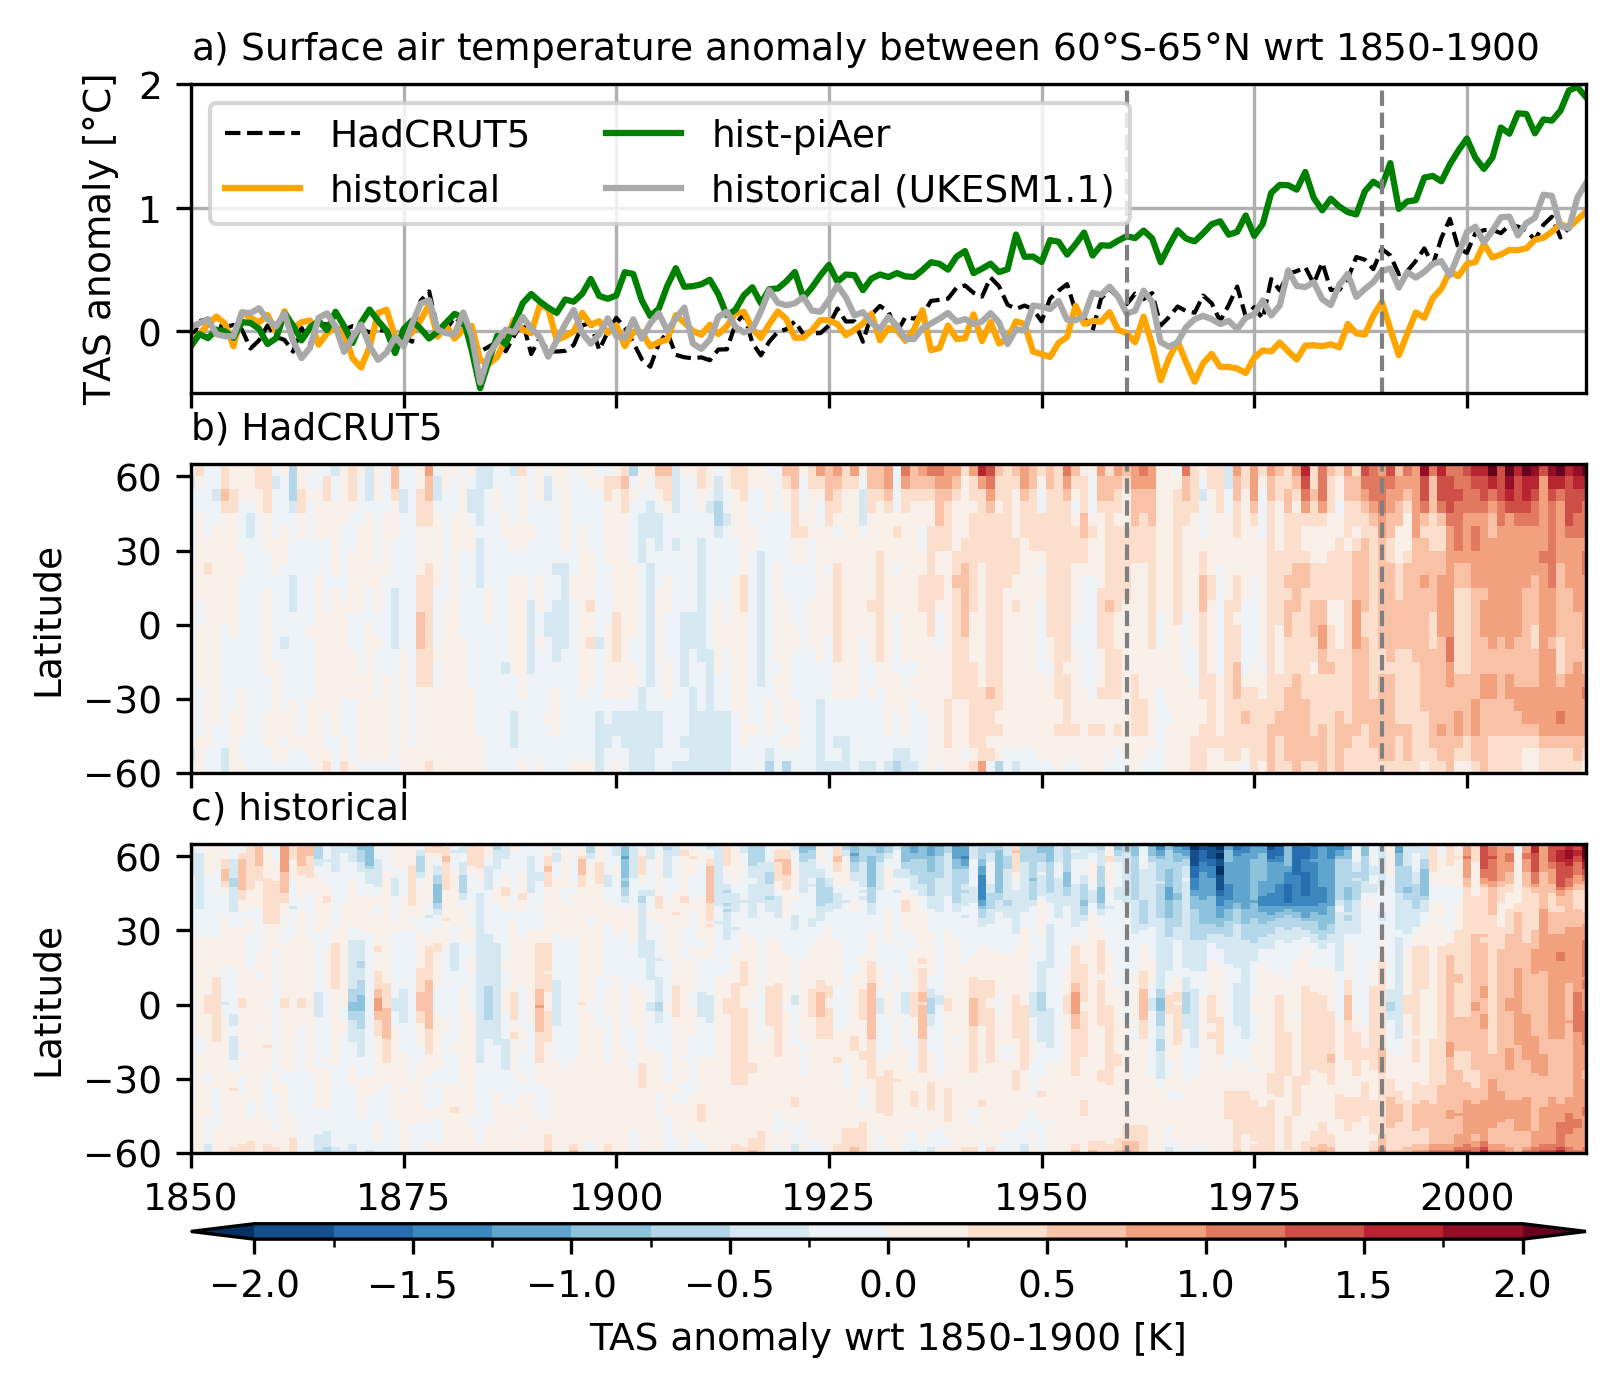
\includegraphics{Chapter4/Figs/TAS_anomaly_cropped.png}
    \caption[Surface air anomaly from HadCRUT5, UKESM1, and UKESM1.1 between 1850 and 2015]{a) Annual mean surface air temperature anomaly between 1850 and 2015 with respect to 1850 to 1859 averaged over latitude 60\textdegree S and 65\textdegree N. b) Surface air temperature anomaly from HadCRUT5 adjusted to 1850--1859. c) surface air temperature from UKESM1 \hist{} simulation. Grey dashed lines are the period between 1960--1989 when the ESMs consistenly underpredict TAS and are called the pothole period.}
    \label{fig:ch4:seasonal-tas-anomaly}
\end{figure}

Figure \ref{fig:ch4:seasonal-tas-anomaly} shows the surface air anomaly from HadCRUT5 and UKESM1.  HadCRUT5 is a gridded dataset of global historical surface temperature anomalies relative to a 1961--1990 reference period. Data are available for each month from January 1850 onwards on a 5 degree grid time series \citep{moriceUpdatedAssessmentSurface2021}. The plot has been readjusted with respect to 1850--1859 climatology to show the temperature evolution and the pothole. Annual mean surface temperature from UKESM1 agrees well with HadCRUT5 both before and after the pothole period with especially cold bias in the Northern Hemisphere. This behaviour is observed amongst other ESMs with varying degree of bias, but not in models with lower complexity. The cause for this behaviour is unclear \citep{zhangRoleAnthropogenicAerosols2021}.

UKESM1 overestimated surface \ce{SO2} concentration which has been thought to related to its dry deposition and cause the pothole cooling \citep{hardacreEvaluationSO2SO422021}. A new version of UKESM1, called UKESM1.1, has recently been released with a higher \ce{SO2} dry deposition to address this challenge \citep{mulcahyUKESM11DevelopmentEvaluation2023}. While the new dry deposition scheme improved the surface air temperature predicton, this has exacerbated the model low bias in \ce{SO4}. Thus, better understanding of chemistry-aerosol-climate interaction is still needed to address the pothole problem.

\subsection{Observed seasonal trend in \ce{SO2} oxidation}
\label{ch4:seasonal-so2-oxidation-observation}

Research on \ce{SO2} primarily focused on its health impacts either as \ce{SO2} gas or contribution to particulate matter \citep[e.g. ][]{meagherSeasonalVariationAtmospheric1983,eatoughConversionSO2Sulfate1994, feichterSimulationTroposphericSulfur1996} \change{ Add this reference https://www.sciencedirect.com/science/article/pii/0004698181902596}. As such, earlier work on \ce{SO2} oxidation has not made the connection between \ce{SO2} oxidation, cloud, and climate until after the work of \citet{twomeyInfluencePollutionShortwave1977} and \citet{albrechtAerosolsCloudMicrophysics1989} on aerosol-cloud feedback has gained traction \change{ add ref on charlson 1991, 1992: https://www.tandfonline.com/doi/abs/10.3402/tellusa.v43i4.11944 https://www.science.org/doi/abs/10.1126/science.255.5043.423  } .  

One of the aspect of \ce{SO2} oxidation that has been observed but not well-studied is the seasonal cycle of the oxidation. Earlier research show that \ce{SO2} conversion rate to sulfate by \ce{SO2 + OH} increases by a factor of 1 between summer and winter \citet{meagherSeasonalVariationAtmospheric1983}. A model study also indicates that the oxidant levels and respective oxidation exhibit a seasonal cycle \citet{feichterSimulationTroposphericSulfur1996}. 

% Evidence that oxidants vary between seasons
According to field studies using instrumented aircraft sampling down-wind air from coal-fired power plants between 1975--1978, the gas-phase \ce{SO2} oxidation has a strong seasonal cycle \citep{meagherSeasonalVariationAtmospheric1983}. The rate of conversion of \ce{SO2} to \ce{SO4^-2} rate varies from a winter low of \qty{1.5E-3}{\per\hour} to a summer high of \qty{1.3E-2}{\per\hour}. 


Conversion rate, $k(\ce{SO4^2-})$, is calculated from
\begin{equation}
k(\ce{SO4^2-}) = \frac{\ce{SO4^2-}]}{([\ce{SO2}]+[\ce{SO4^2-}])t}
\end{equation}
where t is the plume travel time. The plume was sampled at several downwind distances.


In the same study, correlation analysis was also performed between conversion rate and other parameters, including type of power plant and location, time of day, solar intensity, temperature, background \ce{O3} concentration, relative humidity, and specific humidity. Only specific humidity and temperature correlate significantly with the conversion rate. This work suggested that the correlation is due to the seasonal trend rather than a direct relationship of the variable \citep{meagherSeasonalVariationAtmospheric1983}.


% Modelling studies agree with observations
Modelling studies also suggest that there is a 4-fold increase in \ce{SO2 + OH} oxidation between summer and winter which agrees with \ce{SO2} conversion rate at noon at 35 \textdegree N observed as shown in Fig. \ref{fig:ch4:meagher1983} \citep{meagherSeasonalVariationAtmospheric1983}. 

\begin{figure}
    \centering
    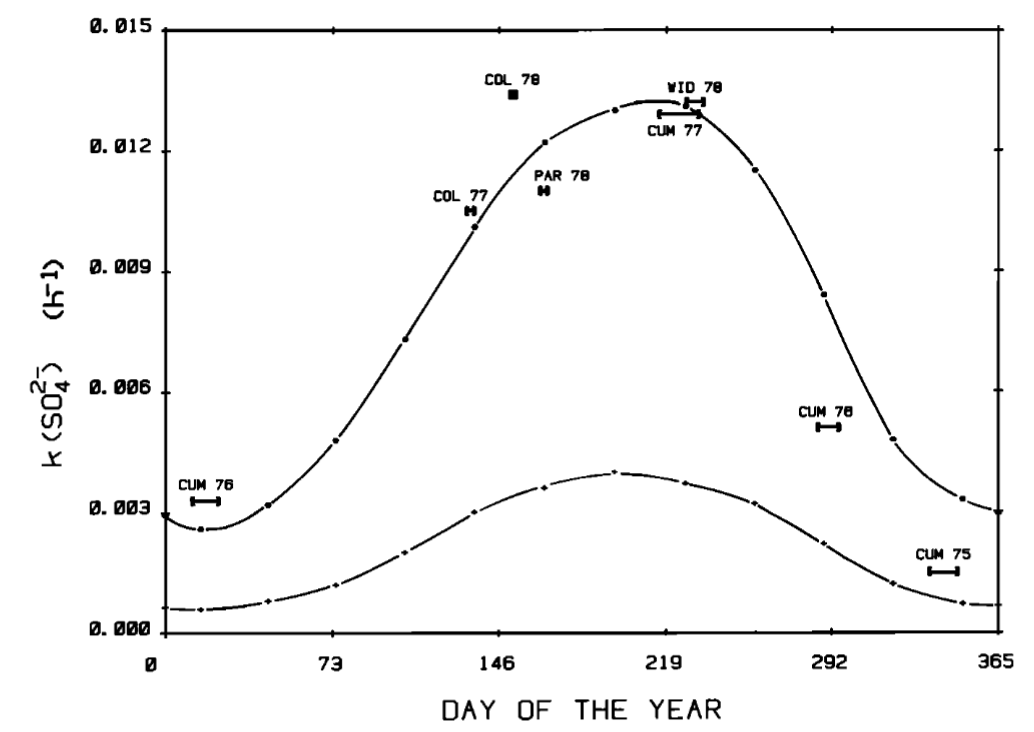
\includegraphics[width=0.8\linewidth]{Chapter4/Figs/meagher1983.png}
    \caption{Average rate of \ce{SO2} conversion to \ce{SO_4^{2-}} measured at different power station plumes. Also shown in this figure are the noontime (top curve) and diurnal average (bottom curve) \cite{meagherSeasonalVariationAtmospheric1983}}
    \label{fig:ch4:meagher1983}
\end{figure}


\ce{SO2 + OH} oxidation is the most important and most rapid during daytime and in summer due to more OH concentration from photochemical reactions \citet{eatoughConversionSO2Sulfate1994}. However, \ce{H2O2} oxidation becomes more important during nighttime or when atmospheric water droplets are present, such as in clouds and fog \cite[e.g. ][]{eatoughConversionSO2Sulfate1994} \change{ Add this reference https://www.sciencedirect.com/science/article/pii/0004698183901816 and https://www.sciencedirect.com/science/article/pii/0004698182903481 and https://agupubs.onlinelibrary.wiley.com/doi/10.1029/91JD01943}. 


Field studies suggest that the aqueous-phase concentration of the oxidant and the reaction kinetics factors, including cloud droplet pH and temperature, are the two important factors influencing the oxidation process \cite{eatoughConversionSO2Sulfate1994}. \ce{SO2} in the gas phase gets dissolved into water droplets along with \ce{O3} and \ce{H2O2}. Both \ce{O3} and \ce{SO2} are moderately soluble in the pH range 3--6, which is the typical atmospheric acidity. Most of the dissolved \ce{SO2} will be present as \ce{HSO3^-} with the concentration of \qty{e-4}{M}. Atmospheric mixing ratio of tropospheric \ce{O3} generally falls in the range between 50-100 ppb, resulting in approximately \num[]{e-9} M. \ce{H2O2} is very soluble, with the atmospheric mixing ratio between 0.1-5 ppb, aqueous concentration is expected at about \qty{e-4}{M} \cite{eatoughConversionSO2Sulfate1994}.


\subsection{Modelling studies showing seasonal trend in \ce{SO2} oxidation and radiative effects}

Most studies in the literature focus on the effects of \ce{SO2} oxidation on air pollution, especially on particulate matter concentration and acid rain \cite[e.g.][]{eatoughConversionSO2Sulfate1994} \change{ Add this reference https://www.sciencedirect.com/science/article/pii/0004698183901816 and https://www.sciencedirect.com/science/article/pii/0004698182903481 and https://agupubs.onlinelibrary.wiley.com/doi/10.1029/91JD01943}. One model study shows a global \ce{SO2} oxidation trend for gas- and aqueous-phase oxidation \cite{feichterSimulationTroposphericSulfur1996}. 

\begin{figure}
    \centering
    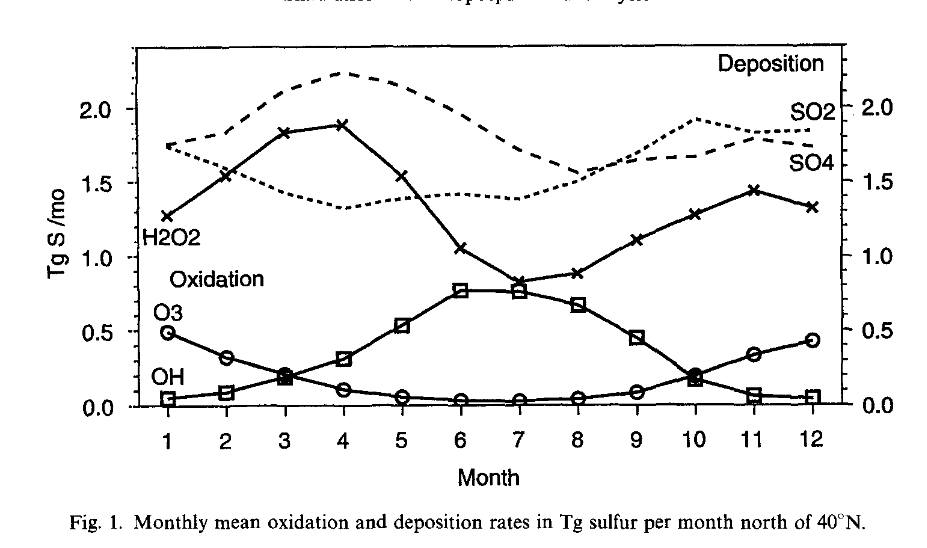
\includegraphics[width=0.8\linewidth]{Chapter4/Figs/feitcher1996.png}
    \caption{Monthly mean \ce{SO2} oxidation and deposition from ECHAM3 \cite{feichterSimulationTroposphericSulfur1996}}
    \label{fig:ch4:feichter1996}
\end{figure}

Figure \ref{fig:ch4:feichter1996} shows the seasonal trend in \ce{SO2} oxidation from general circulation model (CTM) ECHAM3 developed at the Max-Planck Institute for Meteorology. Emission, transport, chemistry and rainout of the sulfur species DMS, S O 2 and sulfate are
calculated on-line with the meteorology in ECMAM3 which offers a high temporal resolution but the spatial resolution is not fine enough to adequately resolve synoptic scale weather patterns. The  model treats DMS and \ce{SO2} as gas, and \ce{SO4^2-} as aerosol, all of which are prognostic variables. During summer months, about half of sulfate aerosols are simulated in cloud and the other half as homogeneous gas-phase reaction. While in winter, most sulfate production occurs in aqueous phase \citep{feichterSimulationTroposphericSulfur1996}.


Recently, seasonal difference of ERF due to aerosols has been quantified \citep{bellouinRegionalSeasonalRadiative2016}. Four models participated in this simulations including three general circulation models: ECHAM6-HAM2, HadGEM3-GLOMAP, NorESM1-M \info{Based on data portal, ECHAM6-1-05-LR, HadGEM2-A/AO/CC/ES, NorESM1-M participated in CMIP5} and one chemical transport model: OsloCTM2. In this study, simulations last one year after spin-up. Emissions from four regions (Europe, East Asia, Rest of the world, and shipping sector) for the year 2008 are reduced by 20\%  to represent feasible emission reduction in two seasons: summer (May--October) and winter (November--April). In case of \ce{SO2} emissions, the perturbations reduce \ce{SO2} emissions by -1.54 and \qty{-1.7}{Tg(S)~yr^{-1}} in Europe, -6.28 and \qty{-6.7}{Tg(S)~yr^{-1}} in East Asia, and -10.2 and \qty{-10.4}{Tg(S)~yr^{-1}} for the rest of the world, in summer and winter, respectively.


\begin{figure}
    \centering
    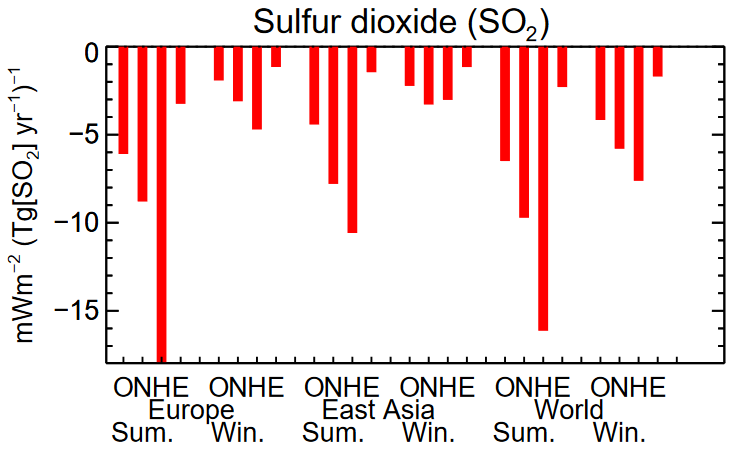
\includegraphics[width=0.5\linewidth]{Chapter4/Figs/bellouin2016.png}
    \caption{ Specific radiative forcing (SRF) given in \unit{(mW~m^{-2})~(Tg(\ce{SO2})~yr^{-1})} for regional and seasonal reduction in \ce{SO2} emissions from four models:  OsloCTM2 (O), NorESM1-M (N), HadGEM3-GLOMAP (H) and ECHAM6-HAM2 (E) \cite{bellouinRegionalSeasonalRadiative2016}}
    \label{fig:ch4:bellouin2016}
\end{figure}

Climate impact of each of the forcing in this studies are normalised by its emission to allow for comparison between emission rates, called the specific RF (SRF), as shown in Figure \ref{fig:ch4:bellouin2016}. HadGEM3-GLOMAP \change{What is the relationship between HadGEM2, HadGEM3-GLOMAP and UKESM1??????? UKESM1 physical model is HadGEM3-GC3.1 but does that mean HadGEM3 is a predecessor to UKESM1??? But Sellar (2019) says  predecessor is HadGEM2-ES......} which is a close relative to UKESM1 shows the largest change in ERF per unit of \ce{SO2} emissions in summer from Europe at \qty{18}{(mW~m^{-2})~(Tg(\ce{SO2})~yr^{-1})} or \qty{0.036}{(W~m^{-2})~(Tg(S)~yr^{-1})}.

Another study compares the sulfur budget across many ESMs, focusing on stratospheric sulfate aerosols \citep{brodowskyAnalysisGlobalAtmospheric2024}. However, there are no discussions on tropospheric sulfate aerosol seasonal trends or seasonal radiative effects.

Despite extensive measurement campaigns in the late 20\textsuperscript{th} century to quantify the changes in \ce{SO2} and its oxidation and recent developments in the radiative effects of aerosols, no studies have linked the seasonality of oxidation to radiative effects.


\subsection{Research opportunities and motivation}

This means \ce{SO2} emission in summer could lead to more aerosol number production compared to winter. As aerosol-cloud interaction depends more strongly on the change in aerosol number, one could hypothesise that the aerosol-cloud interaction would be stronger during summer due to more aerosol numbers. While both measurement and modelling studies have confirmed the seasonal cycle of \ce{SO2} oxidation, there has not been a detailed study of how this change in aerosol formation would affect cloud formation in the historical period. 

UKESM1 simulates both aerosol mass and number independently, making it one of the most robust climate models regarding aerosol simulation. GLOMAP-mode, the aerosol module used in UKESM1, simulates both soluble and insoluble aerosols in four modes: nucleation, Aitken, accumulation, and coarse, and different aerosol types: sulfate, sea salt, organic, dust, and black carbon. It also simulates interaction between modes such as coagulation and condensation and wet and dry deposition. This makes UKESM1 a valuable tool for studying the aerosol properties in different seasons.


\section{Methods and data}

This Chapter examines how \ce{SO2} oxidation in UKESM1 responds to changes in physical and chemical parameters. General information on the model is described in Chapter \ref{ch2:title}.

\subsection{Sulfate production rates in UKESM1}
\label{ch4:sec:so4-prod-rate}

The majority of sulfate aerosols are produced in the atmosphere via oxidation. Approximately 5\% of total sulfate production is from primary emissions, which reflects 2.5\% of anthropogenic \ce{SO2} emissions that are assumed to enter the atmosphere as sulfate aerosols. The other 95\% of sulfate aerosol in UKESM1 are produced in two pathways: gas-phase oxidation of \ce{SO2} and OH, producing sulfuric acid, which nucleates into new particles, and aqueous-phase oxidation in cloud droplets. 

Gas-phase oxidation of \ce{SO2 + OH} is a termolecular reaction, Reaction \ref{ch1:eq:so2-oh}, with the parameters for rate constant given in Table \ref{ch4:tab:so2-oh-reaction-consts} a function of the concentration of air, [M], and temperature, T.
\begin{align}
    \dfrac{d[\ce{SO2}]}{dt} =  k_{([M],T)} [\ce{SO2}][\ce{OH}][\ce{M}] \label{ch4:eq:so2-oh-prod}
\end{align}

The rate constant for the termolecular reaction, $k_{([M],T)}$, is given below.
\begin{align}
    k_0 &= k_1 \left(\frac{T}{300}\right)^{\alpha_1} \exp{(-\beta_1/T)} \label{ch4:eq:so2-oh-k0}\\
    k_\infty &= k_2 \left(\frac{T}{300}\right)^{\alpha_2} \exp{(-\beta_2/T)} \label{ch4:eq:so2-oh-k_inf}\\
    k_{([M],T)} &= \left( \frac{k_0[M]}{1+\frac{k_0[M]}{k_\infty}}\right) F_c^{\left\{ 1+\left[ \log_{10} \left( \frac{k_0[M]}{k_\infty}\right) \right]^2 \right\}^{-1}} \label{ch4:eq:so2-oh-k_MT} 
\end{align}

The free radical \ce{HSO3} reacts in a chain of reactions with \ce{O2} and \ce{H2O} to form \ce{H2SO4}.

\begin{table}[]
\centering
    \begin{tabular}{ccccccccc}
    \hline
    Reactants & Products & $F_c$ & $k_1$ & $\alpha_1$ & $\beta_1$ & $k_2$ & $\alpha_2$ & $\beta_2$ \\ \hline
    \ce{SO2 + OH} & \ce{SO3 + HO2} & 0.60 & 3$\times 10^{-31}$ & -3.3 & 0 & 1.5$\times 10^{-12}$ & 0 & 0 \\ \hline
    \end{tabular}
\caption{constants for \ce{SO2 + OH} reaction}
\label{ch4:tab:so2-oh-reaction-consts}
\end{table}

The aqueous-phase reactions in UKESM1 require information about cloud droplets and cloud droplet acidity as acidity determines rates of \ce{SO2 + O3} and \ce{SO2 + H2O2} reactions \citep{seinfeldAtmosphericChemistryPhysics2016}. Once the reaction rates are determined from Equation \ref{ch1:eq:so2-o3}--\ref{ch1:eq:so2-h2o2}, the in-cloud sulfate aerosol production is obtained from
\begin{align}
    \Delta S_{\mathrm{cloud}} = F \cdot \left( \dfrac{d[S(IV)]}{dt}\right) \cdot L \cdot N_a \cdot \frac{1}{\rho_w} \label{ch4:eq:in-cloud-sulfate-prod}
\end{align}
where $F$ is the cloud fraction, $ \dfrac{d[S(IV)]}{dt}$ is the aqueous-phase reaction rate, $L$ is the cloud liquid water content, $N_a$ is the Avogadro's constant, and $\rho_w$ is the density of water. In the model version used in this work, global cloud pH is set to 4.0 where the local \ce{SO2} mixing ratio exceeds 0.5 ppb, or 5.0 if not.


GLOMAP-mode, the aerosol module simulating aerosol processes in UKESM1, treats aerosol number concentration for each aerosol mode separately with interaction such as coagulation and between modes. The aerosol number for each mode is represented by a log-normal distribution with a geometric mean diameter $\bar{D}$ covering the nucleation ($\bar{D} < 10$ \unit{\nano\metre}), Aitken ($10 \leq \bar{D} < 100$ \unit{\nano\metre}), accumulation ($100 \leq \bar{D} < 1000$ \unit{\nano\metre}), and coarse ($\bar{D} \geq 1000$ \unit{\nano\metre}) mode. The mass concentration of each component, including sulfate, sea salt, black carbon, organic carbon and dust in each mode, is also calculated separately. 


% \subsection{Specific ERF}
% \subsection{Adjusted HadCRUT5}
% \subsection{Seasonal mean surface anomaly}


\subsection{Seasonal cycle of \ce{SO2} emissions}

This Chapter employs the AerChemMIP historical fixed-SST transient simulation results from UKESM1. Both the model and simulation set-up are described in Chapter \ref{ch2:title}. \ce{SO2} emissions follow that of CEDS \citep{HoeslyHistoricalEmissions2017}, which shows the seasonal trends in \ce{SO2} emissions. 

\begin{figure}
    \centering
    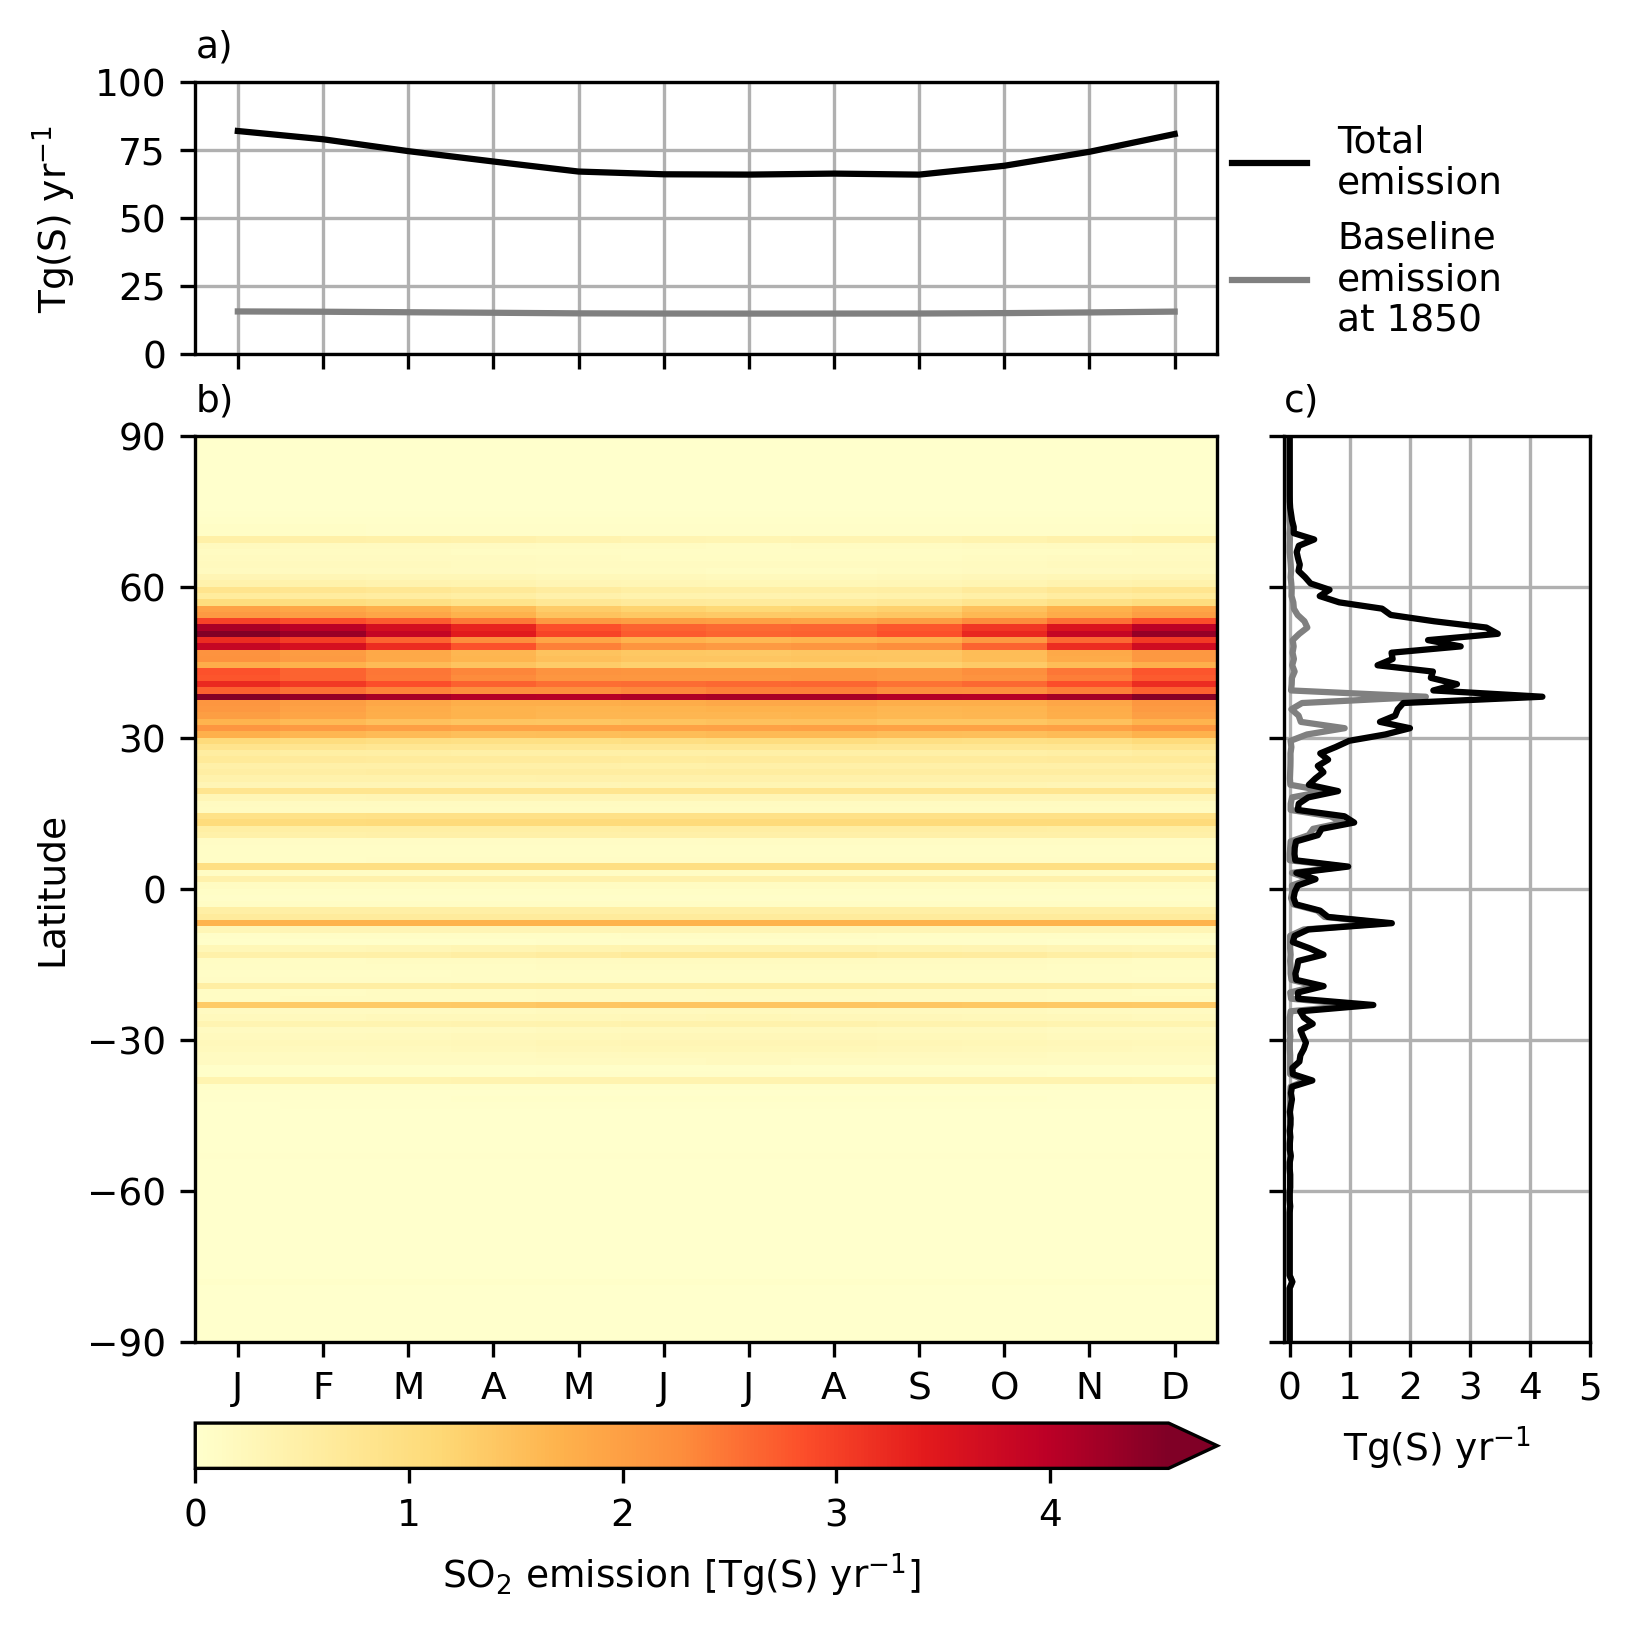
\includegraphics{Chapter4/Figs/emiso2_monthly_pothole.png}
    \caption[Primary \ce{SO2} emissions between 1960 and 1989]{Primary \ce{SO2} emissions between 1960 and 1989. (a) and (c) show total \ce{SO2} emissions from anthropogenic and non-anthropogenic sources at each month and latitude, respectively. (b) shows total emission as a function of month of year and latitude. Baseline emissions are constant and include both anthropogenic and natural emissions.}
    \label{fig:ch4:seasonal-emission}
\end{figure}

Figure \ref{fig:ch4:seasonal-emission} shows primary \ce{SO2} emissions between 1960 and 1989. The anthropogenic emissions rise in the boreal winter as energy usage rises with winter emissions approximately 12.5 \unit{Tg(S)~yr^{-1}} greater than winter's. Most emissions in this period come from fast-growing countries in Europe and North America, accounting for 32.1\% (24.6  \unit{Tg(S)~yr^{-1}}) of the annual mean of 76.6 \unit{Tg(S)~yr^{-1}}. Non-anthropogenic emissions from volcanic degassing contribute to background emissions, which have been constant throughout the years.



\section{Results and discussions}

This Chapter aims to attribute changes in \ce{SO2} oxidation to radiative effects using existing AerChemMIP experiments. The most suitable simulations are the \histsst{} and \sstpiaer, which constrain aerosol precursor emissions at the 1850s level. This poses a challenge for direct attribution as aerosol precursors include not only \ce{SO2} but also precursors for OC and primary BC emissions, making the attribution of changes of \ce{SO2} oxidation to aerosol properties and radiative balance less straightforward. This could be mitigated by selecting suitable periods when \ce{SO2} emissions are significantly greater than OC and BCs. 

A decade between 1960 and 1989 inclusive has been identified for analysis in this Chapter for its high \ce{SO2} emissions and relatively low BC and OC emissions from the main emitting regions: Europe and North America \citep{hoeslyHistorical175020142018}. This period also coincides with the anomalous cooling period. Another period of interest is the near present (2005--2015) when \ce{SO2} emissions increase in Eastern and Southern Asia regions. 

A significant outcome of this Chapter is how changes in seasonal oxidation may modulate the radiative effects of \ce{SO2} emissions with possible effects on the seasonal cycle of surface temperature anomaly. The following needs to be considered when considering the seasonal ERF: the annual cycle of oxidants, sulfate oxidation tendencies, aerosol and cloud properties. The seasonal cycle of ERF and the correlation between oxidation tendencies and aerosol properties are discussed, and changes in ERF per unit of \ce{SO2} emission are quantified. Lastly, this Chapter discusses the correlation between observed seasonal trends in surface temperature anomaly, specifically during the pothole period, and the contribution to temperature changes from aerosols.

\subsection{Seasonal cycle of oxidants}

OH, \ce{O3} and \ce{H2O2} form photochemically in the atmosphere and are involved in oxidising \ce{SO2}. Figure \ref{fig:ch4:seasonal-oxidants} shows global mean oxidant concentrations below 5 km. All oxidants' concentrations strongly correlate to insolation, where maximum concentration follows the solar radiation peaks. \ce{SO2} concentration localises near emission sources and peaks in winter when emissions are more substantial, as shown in Figure \ref{fig:ch4:seasonal-emission}.

\begin{figure}
    \centering
    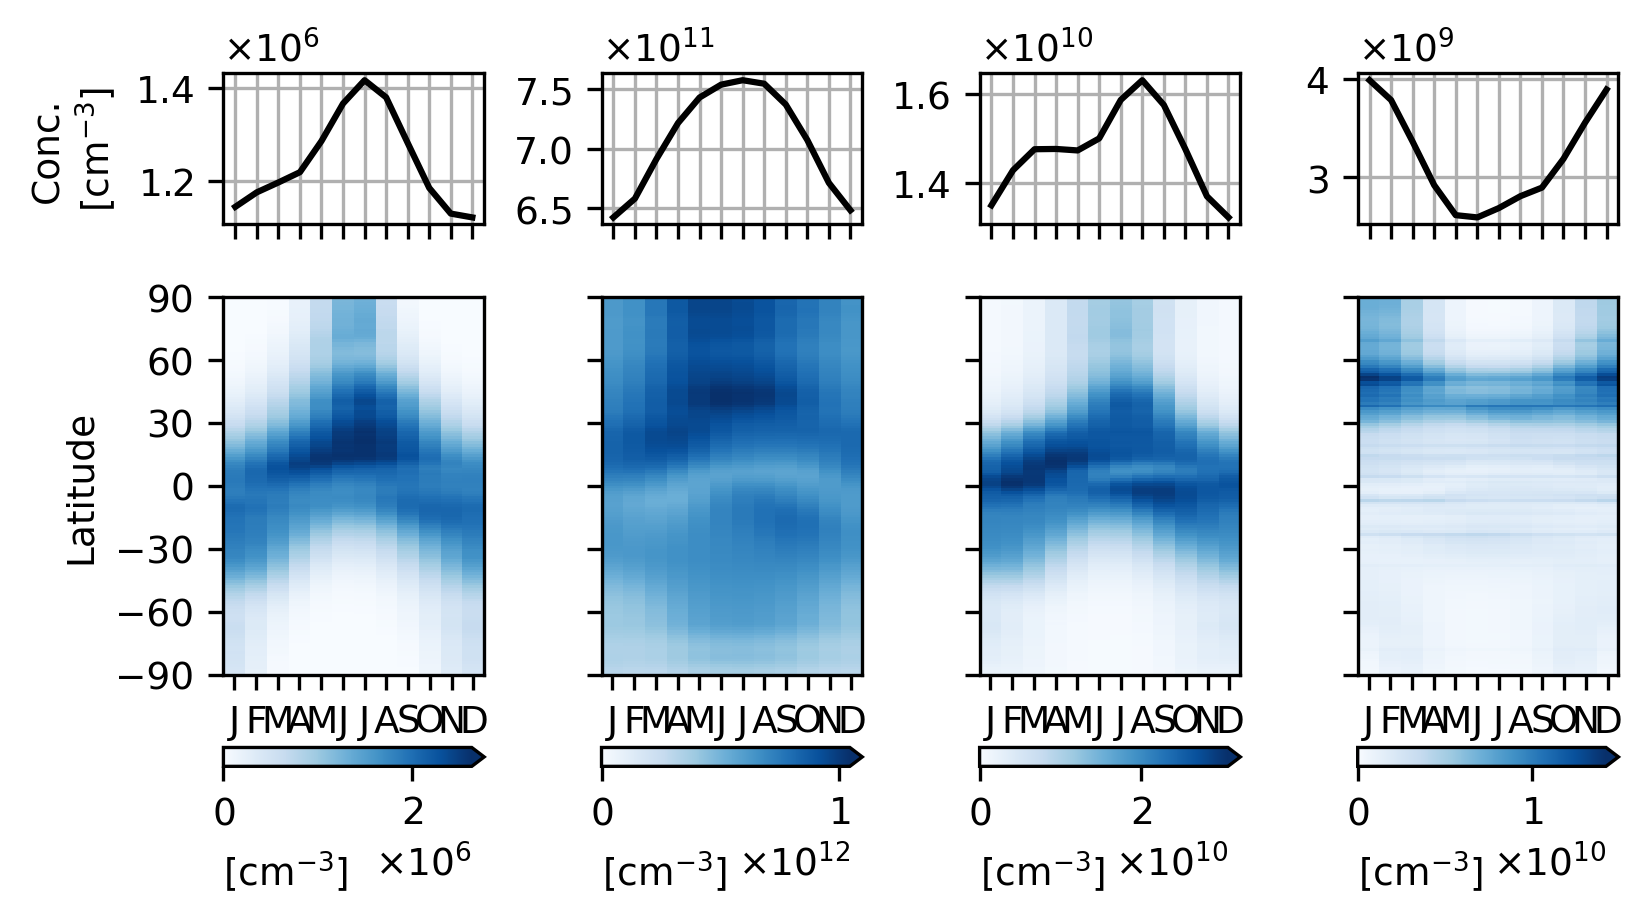
\includegraphics{Chapter4/Figs/seasonal_oxidant_pothole.png}
    \caption[Mean concentration of \ce{OH}, \ce{O3}, \ce{H2O2}, and \ce{SO2} from surface to 5 km between 1960 and 1989]{Global mean concentration of (a) \ce{OH}, (b) \ce{O3}, (c), \ce{H2O2}, and (d) \ce{SO2} from surface to 5 km between 1960 and 1989 as a function of month of year. (e-g) show the respective oxidant concentration as a function of month of year and latitude for the same domain.}
    \label{fig:ch4:seasonal-oxidants}
\end{figure}

Between latitude 30 and 60 \textdegree N where most anthropogenic \ce{SO2} are emitted, OH and \ce{H2O2} concentrations vary greatly between seasons, with their summer concentrations one and two orders of magnitude greater than their respective winter concentrations. OH concentration increases from \num{2.4e5} to \qty{2.1e6}{\per\cubic\cm} and \ce{H2O2} concentration increases from \num{3.0e8} to \qty{2.3e10}{\per\cubic\cm}, as shown in Figure \ref{fig:app1:seasonal-oxidant-30-60}). 

While \ce{O3} concentration between latitude 30 and 60 \textdegree N is also greatest in the boreal summer months, exceeding \qty{1.1e12}{\per\cubic\cm}, its variation is not as drastic, with winter concentration over the same latitude band approximately half that of summer (\qty{7.2e11}{\per\cubic\cm}).

% Discuss SO2 loss via reaction with all the oxidants and refer to the emission seasonal cycle
\ce{SO2} concentration mimics its emission, reaching maximum in winter and minimum in summer. In summer, less \ce{SO2} is emitted, and more is oxidised, leading to a lower concentration and shorter lifetime in summer, discussed in the following section.

\subsection{Seasonal cycle of oxidation}

\begin{figure}
    \centering
    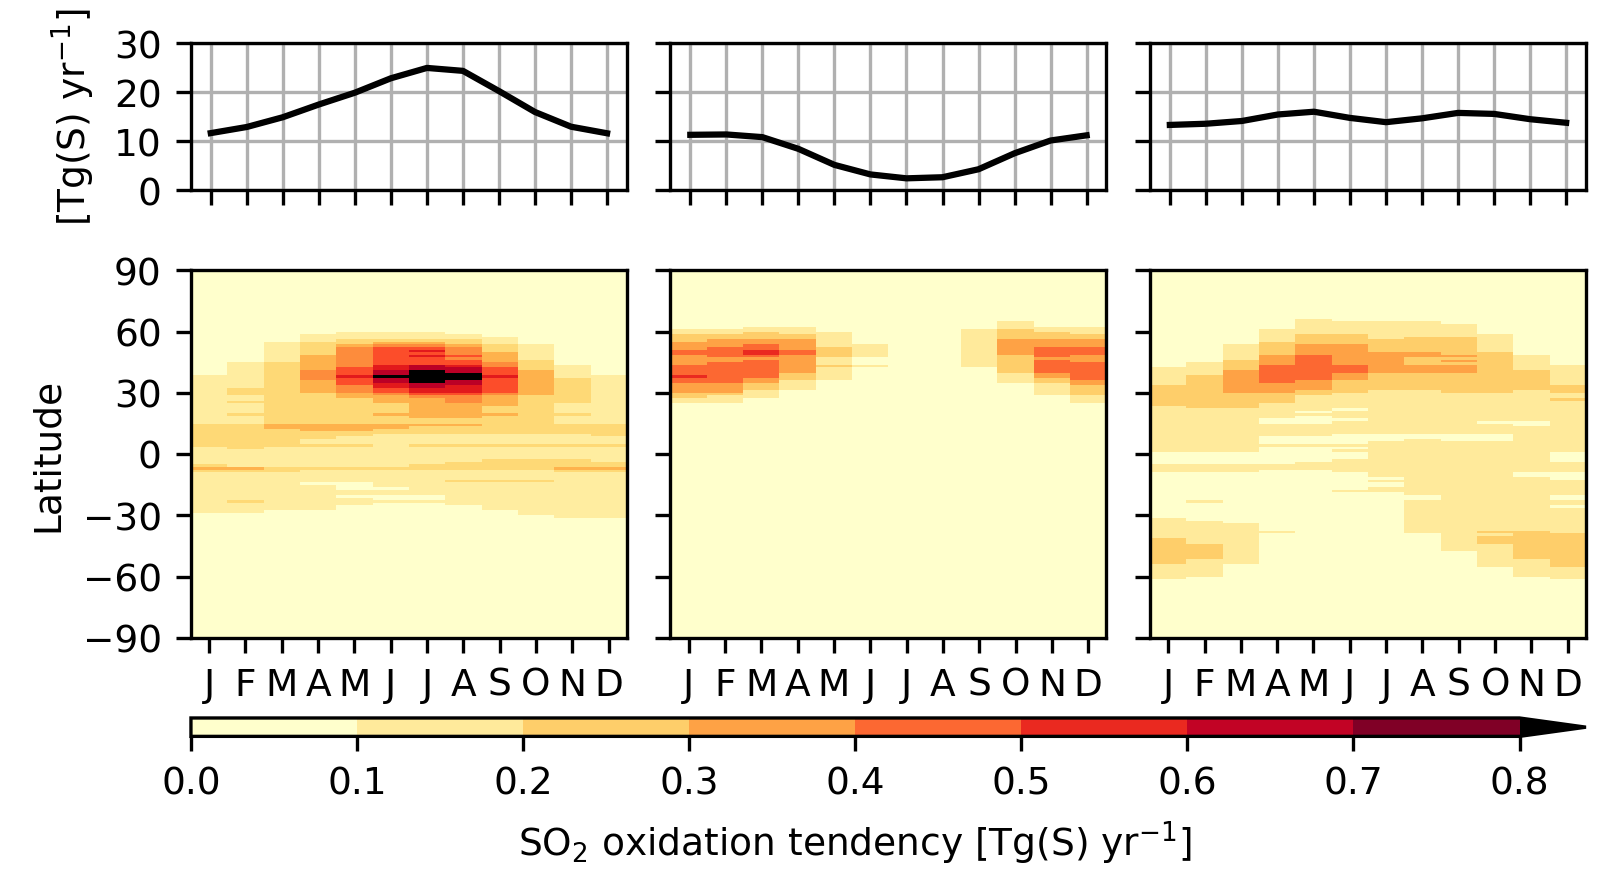
\includegraphics{Chapter4/Figs/seasonal_oxidation_w_summary_histsst_pothole.png}
    \caption[Total tropospheric \ce{SO2} oxidation tendencies as a function of latitude and months between 1960 and 1989]{Total \ce{SO2} oxidation with (a) OH, (b) \ce{O3}, and (c) \ce{H2O2} as a function of months between 1960 and 1989. (d-f) show the respective oxidation tendencies as a function of months and latitude for the same domain.}
    \label{fig:ch4:seasonal-oxidation}
\end{figure}

Figure \ref{fig:ch4:seasonal-oxidation} shows that \ce{SO2 + OH} maximises during boreal summer with a tendency reaching 29 \unit{Tg(S)~yr^{-1}}. This is expected as OH concentration is also high during the same period. However, for aqueous-phase reactions, \ce{SO2 + O3} and \ce{SO2 + H2O2}, the oxidation tendencies do not follow the trends of their respective oxidants. This implies that the concentration levels of \ce{O3} and \ce{H2O2} are not the limiting factor for aqueous-phase oxidation. 

The main difference between gas- and aqueous-phase oxidation lies in their parameterisation. Unlike gas-phase reactions, both \ce{SO2 + O3} and \ce{SO2 + H2O2} take place in cloud droplets. Aqueous-phase oxidation of \ce{SO2} with \ce{O3} and \ce{H2O2} is parameterised in  UKESM1 using Equation \ref{ch4:eq:in-cloud-sulfate-prod}. Multiple processes control the sulfate production rates, each with its limiting parameters. First, the gaseous oxidants dissolve into cloud droplets. This process is limited by the oxidants' Henry's coefficients and their concentrations. The dissolved oxidants react according to reaction rates that depend on the cloud droplet's temperature, pressure, and pH. The amount of available cloud droplets also controls the sulfate production rate as it determines the amount of water in each model grid.

\begin{figure}
    \centering
    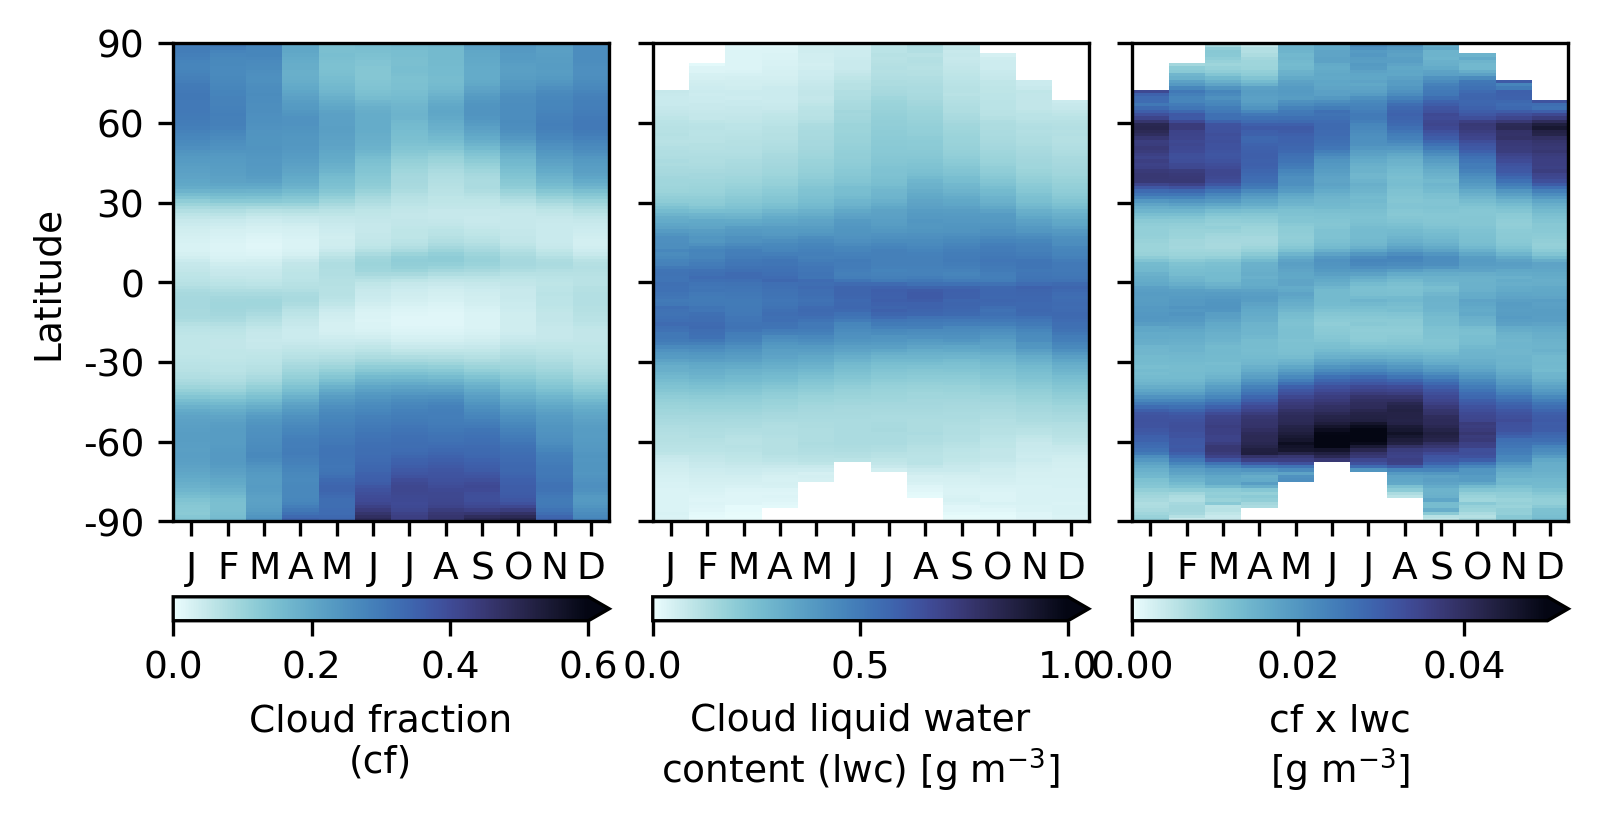
\includegraphics{Chapter4/Figs/seasonal_cf_lwc_histsst_pothole.png}
    \caption[Mean cloud fraction and liquid water content below 10 km between 1960 and 1989]{Mean (a) cloud fraction, (b) liquid water content and (c) products of cloud fraction and liquid water content as a function of latitude and month of the year from the surface up to 10 km between 1960 and 1989.}
    \label{fig:ch4:seasonal-cf-lwc}
\end{figure}

% Define cf and lwc
Cloud processes parameterisation is needed to simulate cloud in Earth System models with coarse grids. Cloud fraction, sometimes referred to as cloud cover, is a parameter which represents the fraction of the total volume of the model grid box that contains any cloud. It is unitless with a value between zero and one. Cloud liquid water content describes the mass of liquid water in a unit volume of air and has the unit of \unit{\gram\per\cubic\metre}.

Both cloud fraction and cloud liquid water content play essential roles in sulfate production in the aqueous phase, enabling the dissolution of gaseous oxidants into cloud droplets. Figure \ref{fig:ch4:seasonal-cf-lwc} shows seasonal trends of both parameters and their products as a function of months and latitude. Higher cloud fraction collocates with lower liquid water content in the mid-latitudes. The products of cloud fraction and liquid water content are greater than \qty{0.03}{\gram\per\cubic\metre} except for summer for mid-latitude, which explains the lower aqueous-phase reaction during the same season. 

The following sub-section explores the theoretical range of all oxidation pathways due to variations in temperature, cloud droplet pH, and cloud fraction to confirm the modelled observation.

\subsubsection{Theoretical range of \ce{SO2} oxidation reaction rates}

In this section, I quantify the factors that limit sulfate production rates in summer and winter conditions by calculating the rates from equations in UKESM1 using parameter values from observation or model averages. 

The equations describing sulfate production includes Equation \ref{ch4:eq:so2-oh-prod}--\ref{ch4:eq:so2-oh-k_MT} for gas-phase reactions, and Equation \ref{ch1:eq:Henry-eq}--\ref{ch1:eq:aq-conc} and \ref{ch4:eq:in-cloud-sulfate-prod} for aqueous-phase reactions. The parameters needed for the gas-phase reaction include concentration of OH and \ce{SO2}, atmospheric temperature and pressure. Aqueous-phase productions by \ce{O3} and \ce{H2O2} are more complex and require cloud parameters, including cloud fraction, liquid water content and cloud pH, in addition to oxidant concentrations, atmospheric temperature and pressure. 


\begin{figure}
    \centering
    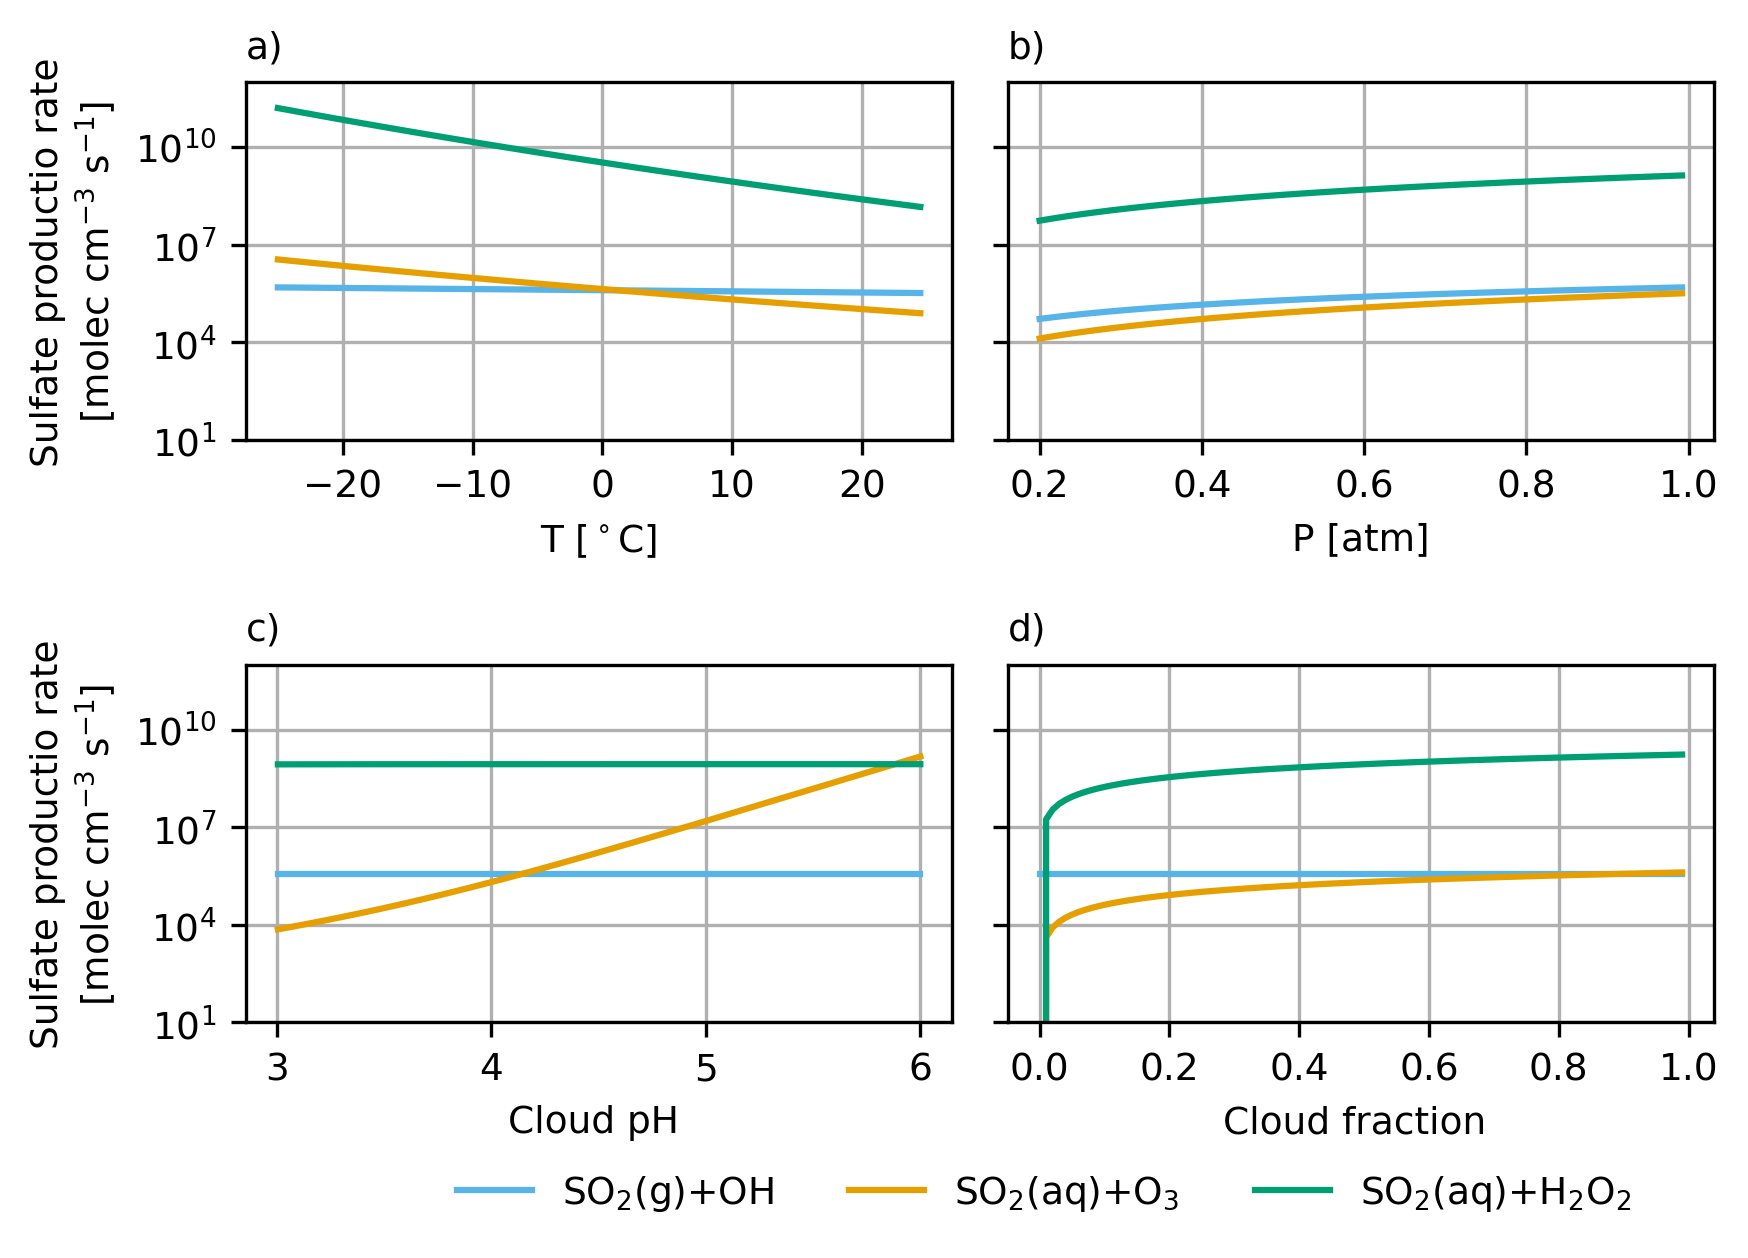
\includegraphics{Chapter4/Figs/oxidation_sensitivity.png}
    \caption[\ce{SO2} oxidation range]{\ce{SO4} production rates for a range of a) atmospheric temperature, b) pressure, c) cloud pH and d) cloud fraction when other parameters are set to average values shown in the first three rows in Table \ref{ch4:tab:sensitivity-test}.}
    \label{fig:ch4:oxidation-sensitivity}
\end{figure}

Changes in sulfate production rates due to temperature, pressure, cloud pH and cloud fraction are shown in Figure \ref{ch4:tab:sensitivity-test}. \ce{SO2 + O3} produces sulfate faster than \ce{SO2 + OH} when the temperature drops below zero \textdegree C, a condition more common in winter and at higher altitudes. Cloud pH strongly influences \ce{SO2 + O3}. \ce{SO2 + O3} oxidation is slower than all other reactions by approximately one order of magnitude except when cloud pH equals 6.0. In this case, \ce{SO2 + O3} reaction rate is the same magnitude as \ce{SO2 + H2O2}. However, this pH is not present in UKESM1 as cloud pH is set to 4.0 or 5.0, depending on the concentration of \ce{SO2}. This thus limits the importance of \ce{SO2 + O3}. Cloud properties do not affect \ce{SO2 + OH} since it is a gas-phase reaction, whereas the aqueous-phase reactions are strongly dependent on cloud fractions, especially when the cloud fraction is below 0.1. 


\begin{table}[]
\centering
\begin{tabular}{p{1.8cm} p{1cm} p{1.25cm} p{1cm} p{1cm} p{0.8cm} p{1cm} p{1cm} p{1cm} p{1cm}}
\toprule
 & \ce{SO2} [ppb] & OH conc. [cm$^{-3}$] & \ce{O3} [ppb] & \ce{H2O2} [ppb] & pH & T [\textdegree C] & P [atm] & CF & LWC [kg m$^{-3}$] \\ \midrule
Average value & 20.0 & 1.0$\times 10^{6} $ & 40.0 & 2.0 & 4.0 & 10.0 & 0.8 & 0.5 & 0.0002 \\
% Minimum & 5.0 & 1.0$\times 10^{5} $ & 20.0 & 0.2 & 3.0 & -25.0 & 0.2 & 0.01 & 0.0002 \\
% Maximum & 50.0 & 5.0$\times 10^{7} $ & 120.0 & 4.6 & 6.0 & 25.0 & 1.0 & 1.0 & 0.0002 \\ 
\midrule
Summer average & 5.0 & 1.0$\times 10^{6} $ & 60.0 & 2.0 & 4.0 & 15.0 & 0.8 & 0.01 & 0.0002 \\
Summer daytime & 20.0 & 5.0$\times 10^{7} $ & 110.0 & 4.6 & 4.0 & 25.0 & 0.8 & 0.01 & 0.0002 \\
Summer nighttime & 10.0 & 3.0$\times 10^{5} $ & 40.0 & 0.1 & 4.0 & 10.0 & 0.8 & 0.01 & 0.0002 \\ \midrule
Winter average & 50.0 & 5.0$\times 10^{5} $ & 30.0 & 1.0 & 4.0 & 0.0 & 0.8 & 0.5 & 0.0002 \\
Winter daytime & 70.0 & 1.0$\times 10^{6} $ & 55.0 & 2.4 & 4.0 & 5.0 & 0.8 & 0.5 & 0.0002 \\
Winter nighttime & 20.0 & 1.0$\times 10^{5} $ & 20.0 & 0.1 & 4.0 & -5.0 & 0.8 & 0.5 & 0.0002 \\ \midrule
Annual average & 20.0 & 1.0$\times 10^{6} $ & 30.0 & 1.0 & 4.0 & 10.0 & 0.8 & 0.1 & 0.0002 \\
Annual daytime average & 20.0 & 1.0$\times 10^{7} $ & 60.0 & 2.0 & 4.0 & 15.0 & 0.8 & 0.1 & 0.0002 \\
Annual nighttime average & 20.0 & 1.0$\times 10^{5} $ & 20.0 & 0.1 & 4.0 & 5.0 & 0.8 & 0.1 & 0.0002 \\ \midrule
UKESM1 summer & 0.1 & 1.4$\times 10^{6} $ & 37.6 & 0.8 & 4.0 & 10.0 & 0.8 & 0.01 & 0.0002 \\
UKESM1 winter & 0.2 & 1.1$\times 10^{6} $ & 31.3 & 0.7 & 4.0 & 10.0 & 0.8 & 0.5 & 0.0002 \\
UKESM1 annual average & 0.2 & 1.3$\times 10^{6} $ & 34.4 & 0.8 & 4.0 & 10.0 & 0.8 & 0.1 & 0.0002 \\ \bottomrule
\end{tabular}
\caption[Parameters for oxidation rates]{Parameters for oxidation rate. CF is cloud fraction, and LWC is liquid water content. Summer, winter, and annual daytime and nighttime averages are taken from field campaigns with similar characteristics (urban areas) where possible. UKESM1 data are taken from Figure \ref{fig:ch4:seasonal-oxidants}, which are monthly mean values.}
\label{ch4:tab:sensitivity-test}
\end{table}


% Describe the oxidant values from different measurement campaigns
The ranges of the sulfate production rates in summer and winter are calculated using oxidant concentrations from different measurement campaigns listed in Table \ref{ch4:tab:sensitivity-test}. \ce{SO2} concentrations are from an urban area in Beijing, China \citep{linCharacteristicsRecentTrends2012}. OH concentrations are taken from two measurement campaigns to cover nighttime and daytime from an urban site in Birmingham, UK \citep{heardHighLevelsHydroxyl2004, khanNighttimeNO3OH2008}. \ce{H2O2} concentrations are taken from rural measurements in Guangzhou, China \citep{huaAtmosphericHydrogenPeroxide2008}. The cloud pH is set to 4.0 as the aerosol module in UKESM1 uses a cloud pH of 4.0 when the concentration of \ce{SO2} is greater than 0.5 ppb \citep{mannDescriptionEvaluationGLOMAPmode2010}. Pressure, cloud fraction and liquid water content are treated as constants.

\begin{figure}
    \centering
    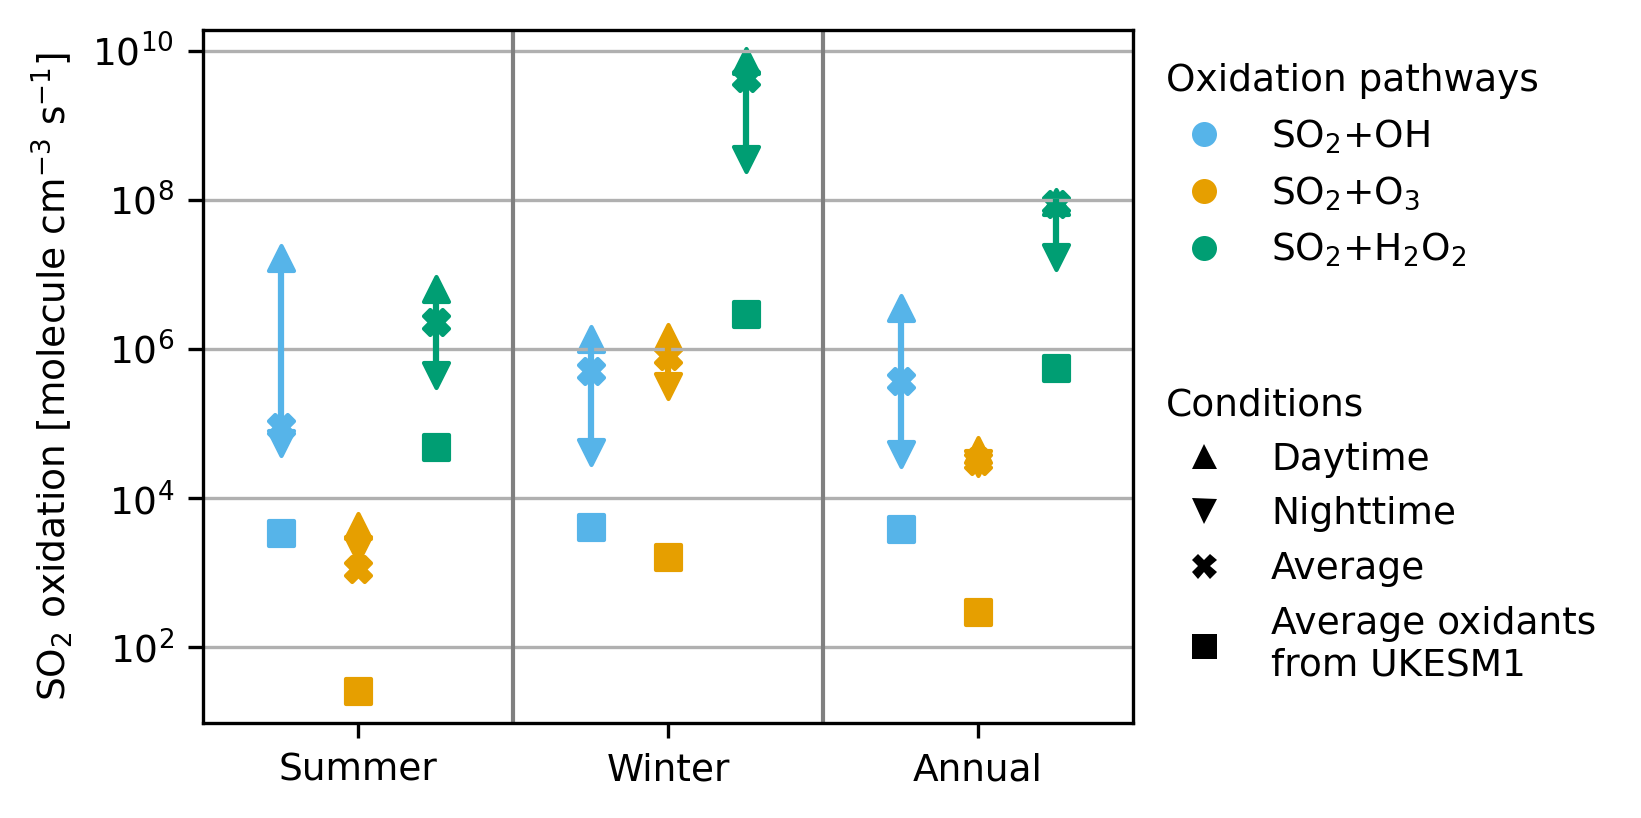
\includegraphics{Chapter4/Figs/theoretical_oxidation.png}
    \caption[\ce{SO4} production rates calculated for summer, winter, and average conditions]{\ce{SO4} production rates calculated for summer, winter, and average conditions as given in Table \ref{ch4:tab:sensitivity-test}.}
    \label{fig:ch4:sensitivity-summary}
\end{figure}

% Explain summer trends for OH
Figure \ref{fig:ch4:oxidation-sensitivity} shows the range of \ce{SO2} oxidation reaction rate in summer and winter using conditions from Table \ref{ch4:tab:sensitivity-test}. \ce{SO2 + OH} is the greatest of all pathways in summer when the temperature and OH concentration are high while the cloud fraction is low. Oxidation by \ce{O3} is the weakest due to low cloud fraction and high temperature. \ce{SO2 + OH} is lower in winter due to lower OH concentration while temperature has negligible effects, as shown in Figure \ref{fig:ch4:oxidation-sensitivity}. 

In contrast, aqueous-phase production by \ce{O3} and \ce{H2O2} increases by two orders of magnitudes in winter compared to summer conditions, placing \ce{SO2 + O3} in the same order of magnitude of \ce{SO2 + OH}. This increase in aqueous-phase production in winter comes from more significant cloud fractions. 

% Comment and compare to other seasonal studies, especially those referenced in the introduction
Comment and compare to other seasonal studies, especially those referenced in the introduction.

The relationship between cloud fraction and aqueous-phase production rate explains the seasonal trends observed in Figure \ref{fig:ch4:seasonal-oxidation}. These results illustrate that cloud property improves aerosol-cloud-climate interaction in UKESM1 and other ESMs. 


\subsection{Sulfur budgets by season}

Oxidation is not the only process that influences the amount of aerosol in the atmosphere. \ce{SO2} may be removed by deposition before it is oxidised into \ce{SO4}. Once oxidised, \ce{SO4} also undergoes deposition, removing it from the atmosphere. All loss processes play a part in determining the lifetime of both sulfur species. This section explores the importance of deposition in determining the sulfur budget and its variation over the year.


\begin{figure}
    \centering
    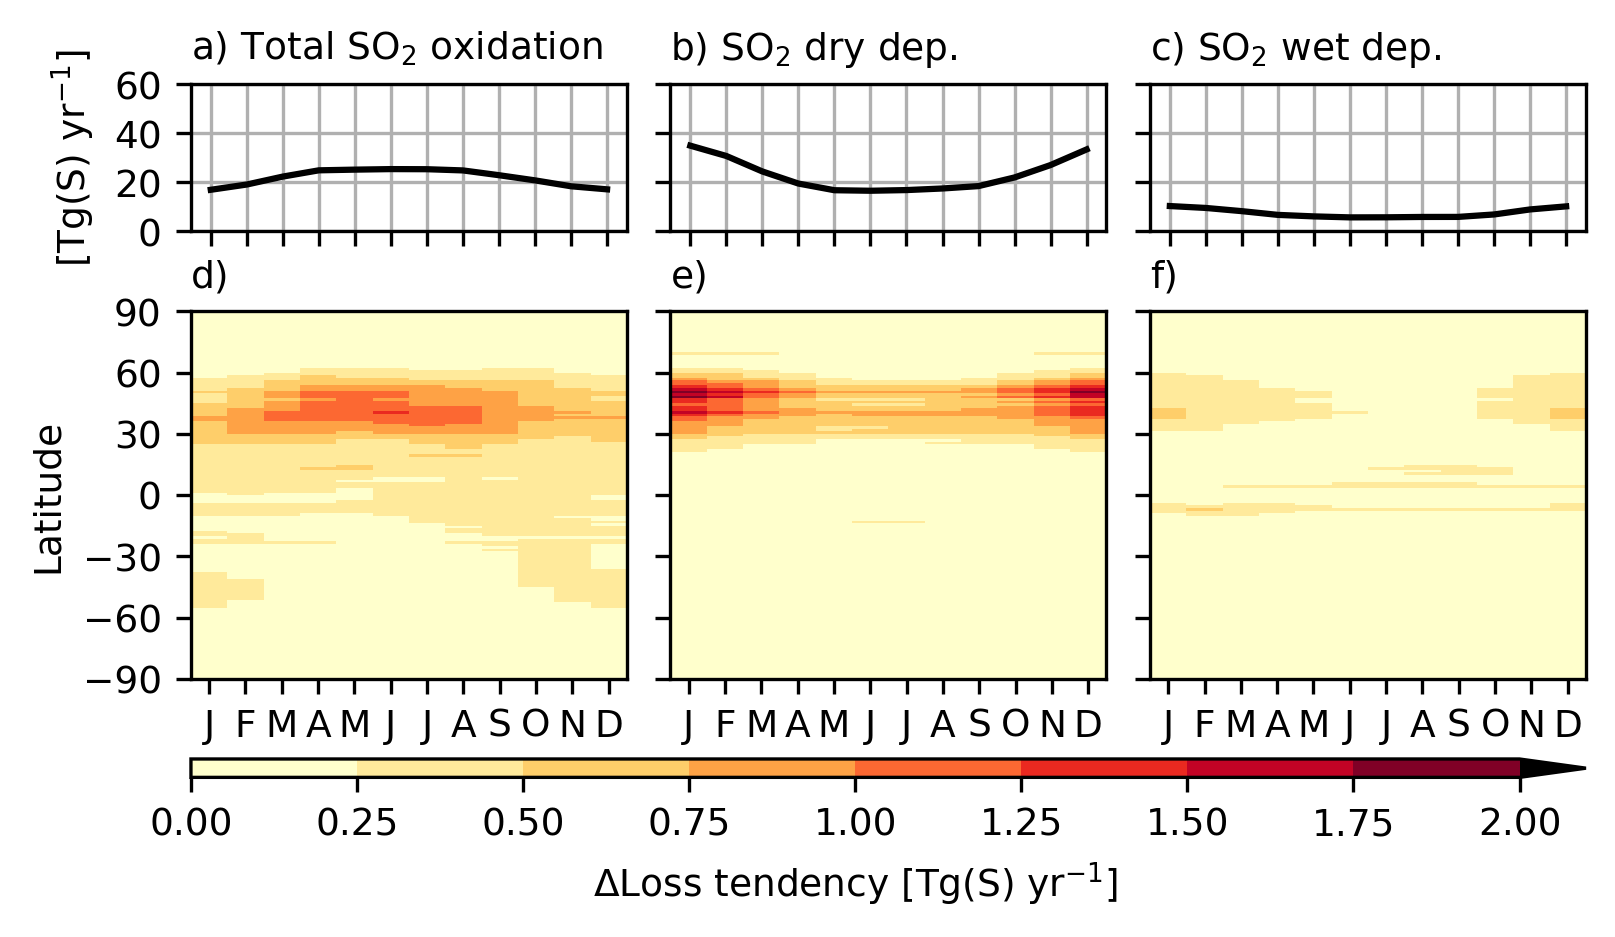
\includegraphics{Chapter4/Figs/so2_losses_histsst_pothole.png}
    \caption[\ce{SO2} loss tendencies due to oxidation and deposition by months between 1960 and 1989 due to aerosol precursor emissions]{\ce{SO2} loss tendencies due to oxidation and deposition by months 1960 and 1989. (a-c) Total seasonal \ce{SO2} loss tendency. (d-f) \ce{SO2} loss tendency as a function of month of year and latitude. This plot is a difference between \histsst{} and \sstpiaer}
    \label{fig:ch4:so2-loss}
\end{figure}


Figure \ref{fig:ch4:so2-loss} illustrates the change in \ce{SO2} losses due to aerosol precursor emissions in 1960--1989 compared to 1850--1859 (\histsst{} minus \sstpiaer{}). Dry deposition removes anthropogenic \ce{SO2} near emission sources along the latitude band between 30 and 60 \textdegree N. Dry deposition is greater in boreal winter when there is more emission than in winter (40 \unit{Tg(S)~yr^{-1}} compared to 20 \unit{Tg(S)~yr^{-1}}). Wet deposition is the lowest of all loss processes, with an annual mean tendency of 10 \unit{Tg(S)~yr^{-1}} in January. Wet and dry deposition correlates with emission trends (high emissions in boreal winter), but oxidants and cloud properties explain the chemical production.


% \begin{figure}
%     \centering
%     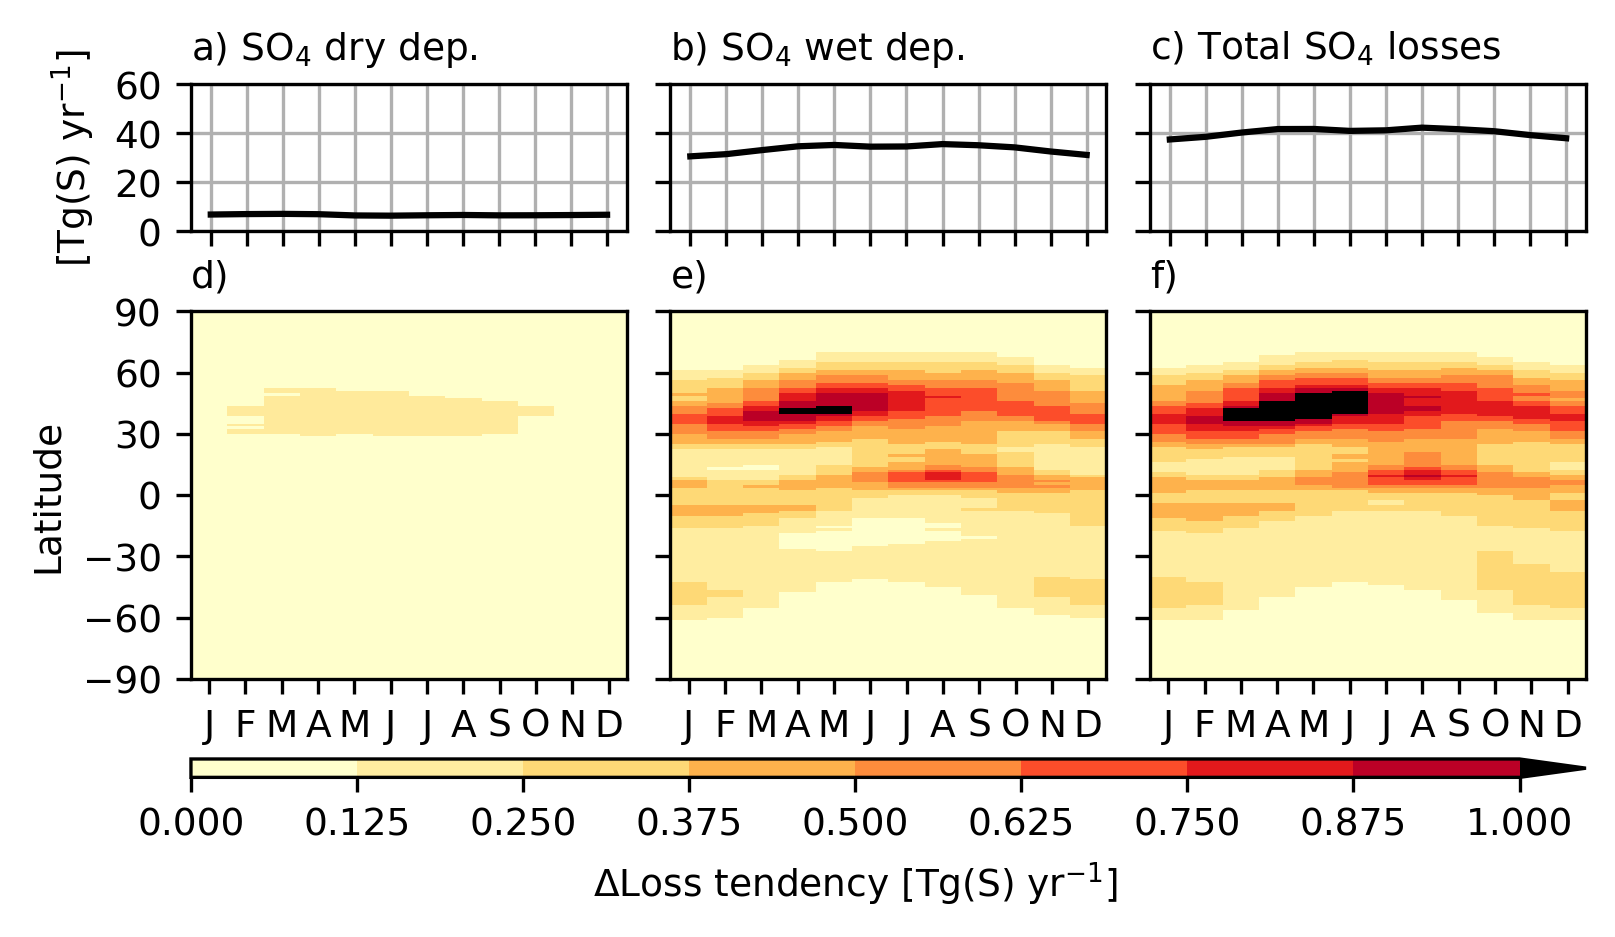
\includegraphics{Chapter4/Figs/so4_losses_histsst_pothole.png}
%     \caption[\ce{SO4} loss tendencies due to oxidation and deposition by months between 1960 and 1989 due to aerosol precursor emissions]{\ce{SO4} loss tendencies due to oxidation and deposition by months 1960 and 1989. (a-c) Total seasonal \ce{SO4} loss tendency. (d-f) \ce{SO4} loss tendency as a function of month of year and latitude. This plot is a difference between \histsst{} and \sstpiaer}
%     \label{fig:ch4:so2-loss}
% \end{figure}



\begin{figure}
    \centering
    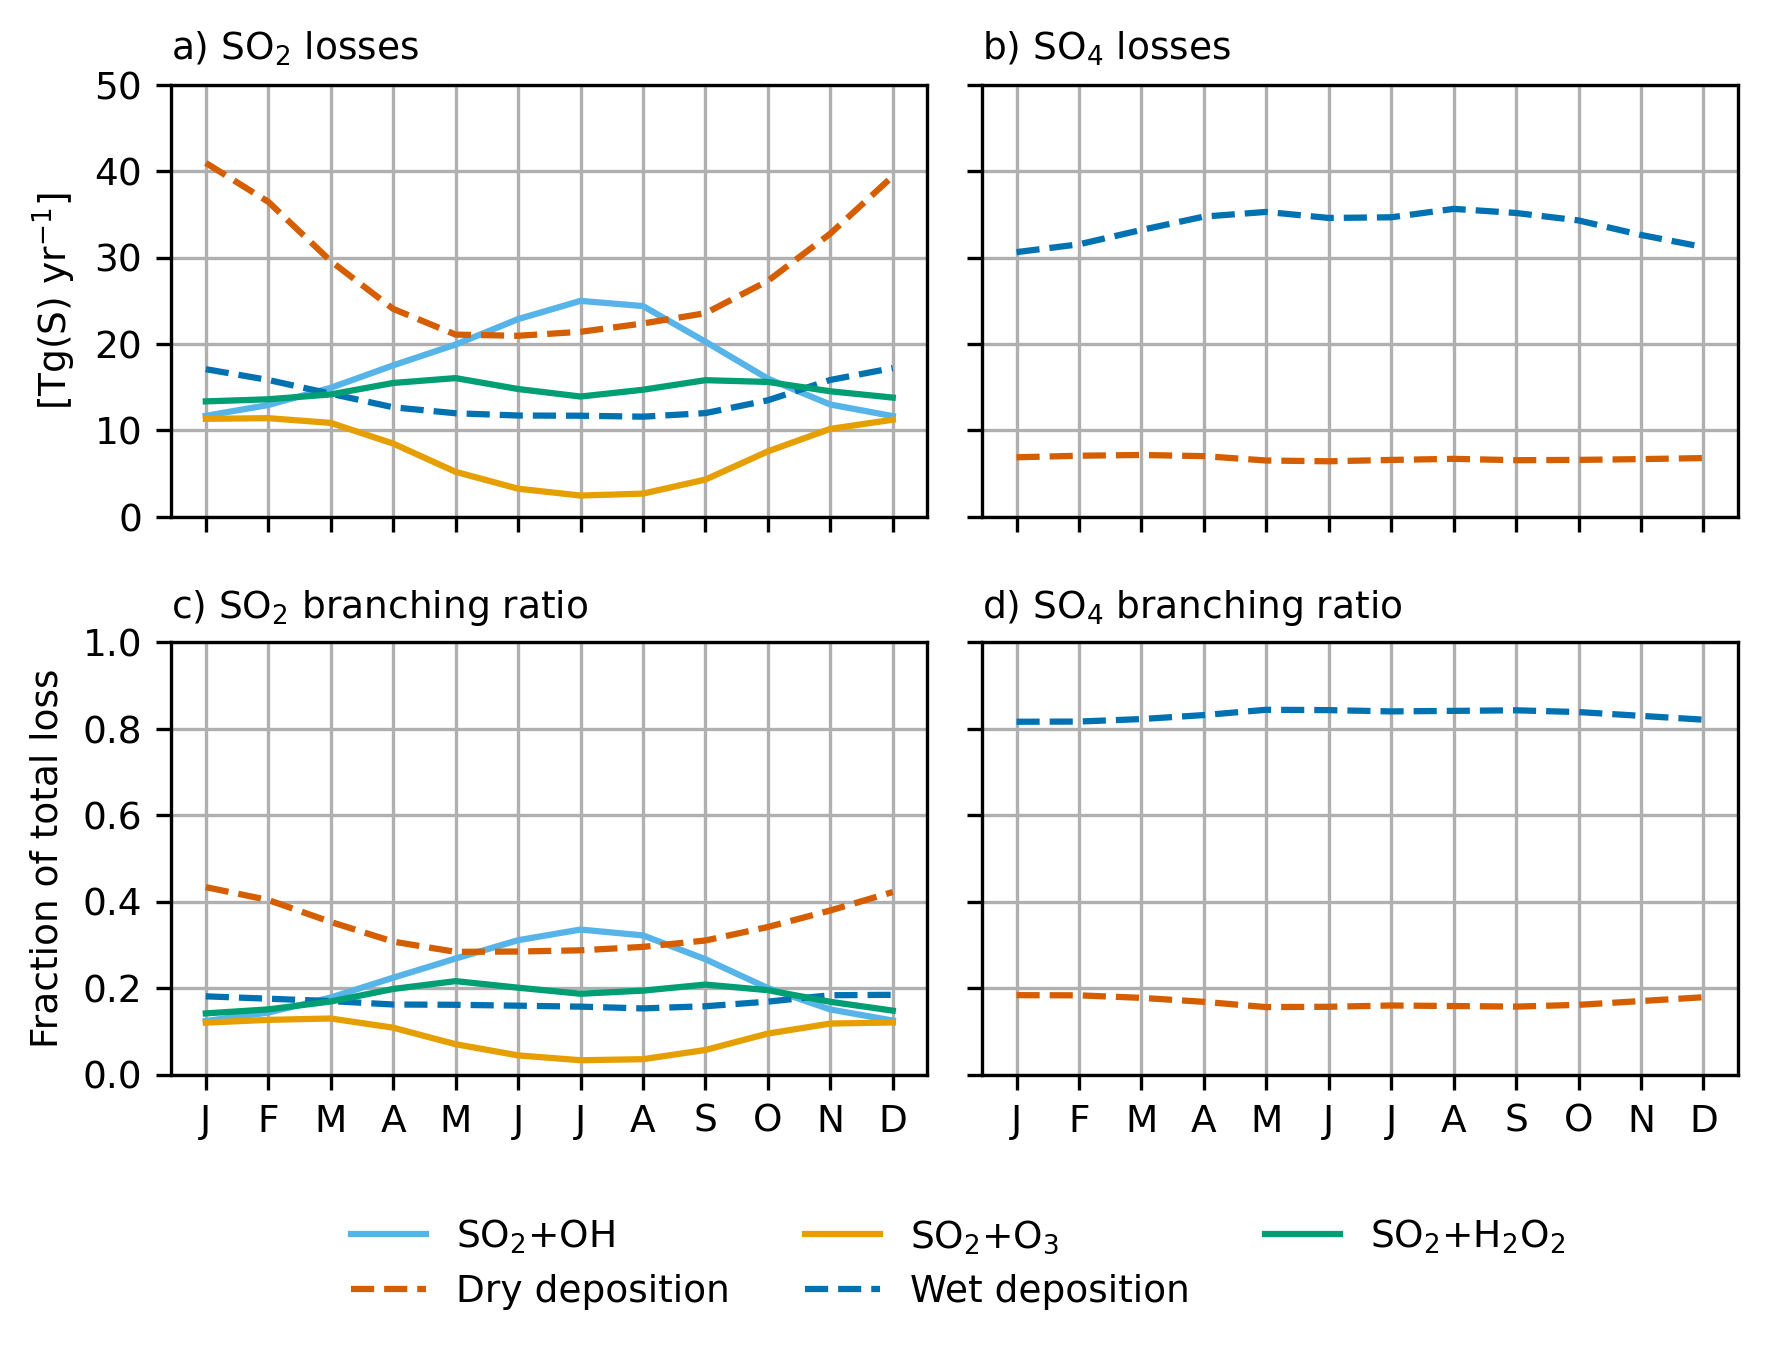
\includegraphics{Chapter4/Figs/branching_ratio_histsst_pothole.png}
    \caption[Absolute and relative losses for \ce{SO2} and \ce{SO4} by month of year between 1960 and 1989]{Absolute and relative losses for \ce{SO2} and \ce{SO4} by month of year between 1960 and 1989. (a-b) Total seasonal \ce{SO2} and \ce{SO4} loss tendency. (c-d) \ce{SO2} and \ce{SO4} loss tendency relative to total losses.}
    \label{fig:ch4:seasonal-branching-ratio}
\end{figure}


Figure \ref{fig:ch4:seasonal-branching-ratio} shows the loss tendencies of \ce{SO2} and \ce{SO4} aggregated by month. It shows that \ce{SO2} may have a different fate depending on the emitted month. During the boreal summer months, 35\% of \ce{SO2} is oxidised by OH, surpassing dry deposition. \ce{SO2 + O3} shows large, but opposite trend to \ce{SO2 +OH}, seasonal variation, contributing less than 10\%  in summer and reaching 15\% in winter. The trend of wet deposition follows emissions, and the fraction of the total loss to which it contributes is largely constant at 18\%. As more \ce{SO2} oxidises and forms \ce{SO4} in summer, \ce{SO4} losses also increase in the same season. However, the ratio between \ce{SO4} wet and dry deposition is relatively constant throughout the year.


\begin{figure}
    \centering
    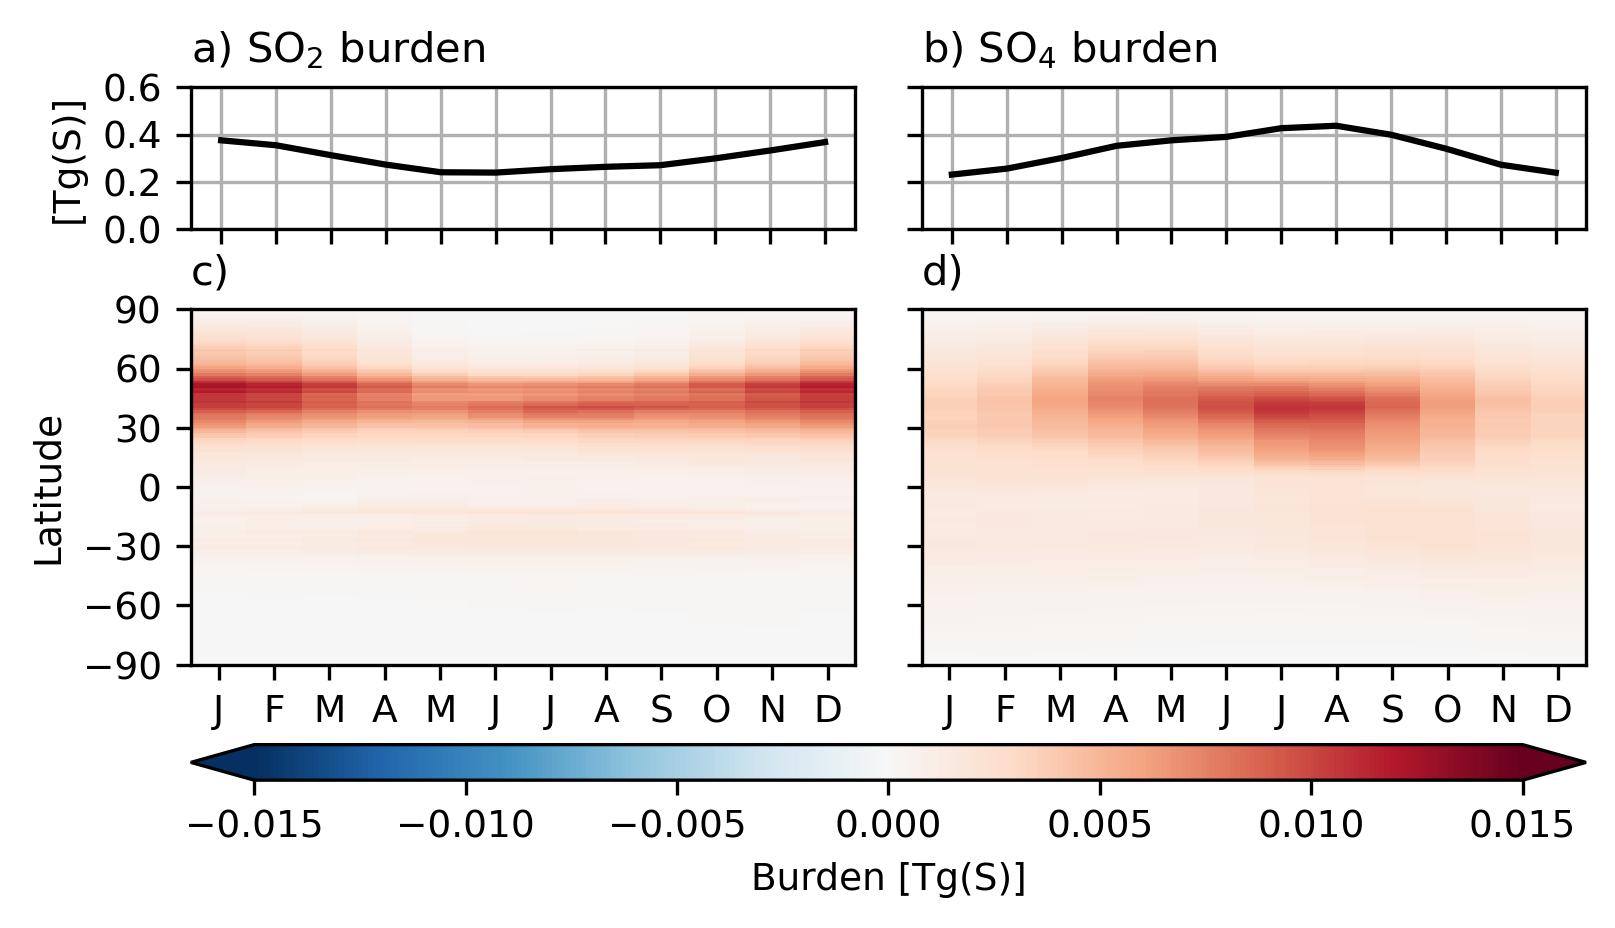
\includegraphics{Chapter4/Figs/seasonal_s_burden_pothole.png}
    \caption[\ce{SO2} and \ce{SO4} mass burden by season between 1960 and 1989]{\ce{SO2} and \ce{SO4} mass burden by season between 1960 and 1989 due to aerosol precursor emissions.}
    \label{fig:ch4:seasonal-s-burden}
\end{figure}

Figure \ref{fig:ch4:seasonal-s-burden} shows the change in \ce{SO2} and \ce{SO4} mass burden due to aerosol precursor emissions. In the northern hemisphere, where emissions are low and oxidation is high in summer, there is a 0.15 Tg(S) decrease in \ce{SO2} burden and subsequent increase in \ce{SO4} burden. The opposite is true when more \ce{SO2} is emitted in boreal winter, resulting in higher \ce{SO2} burden in December and January. 


\begin{figure}
    \centering
    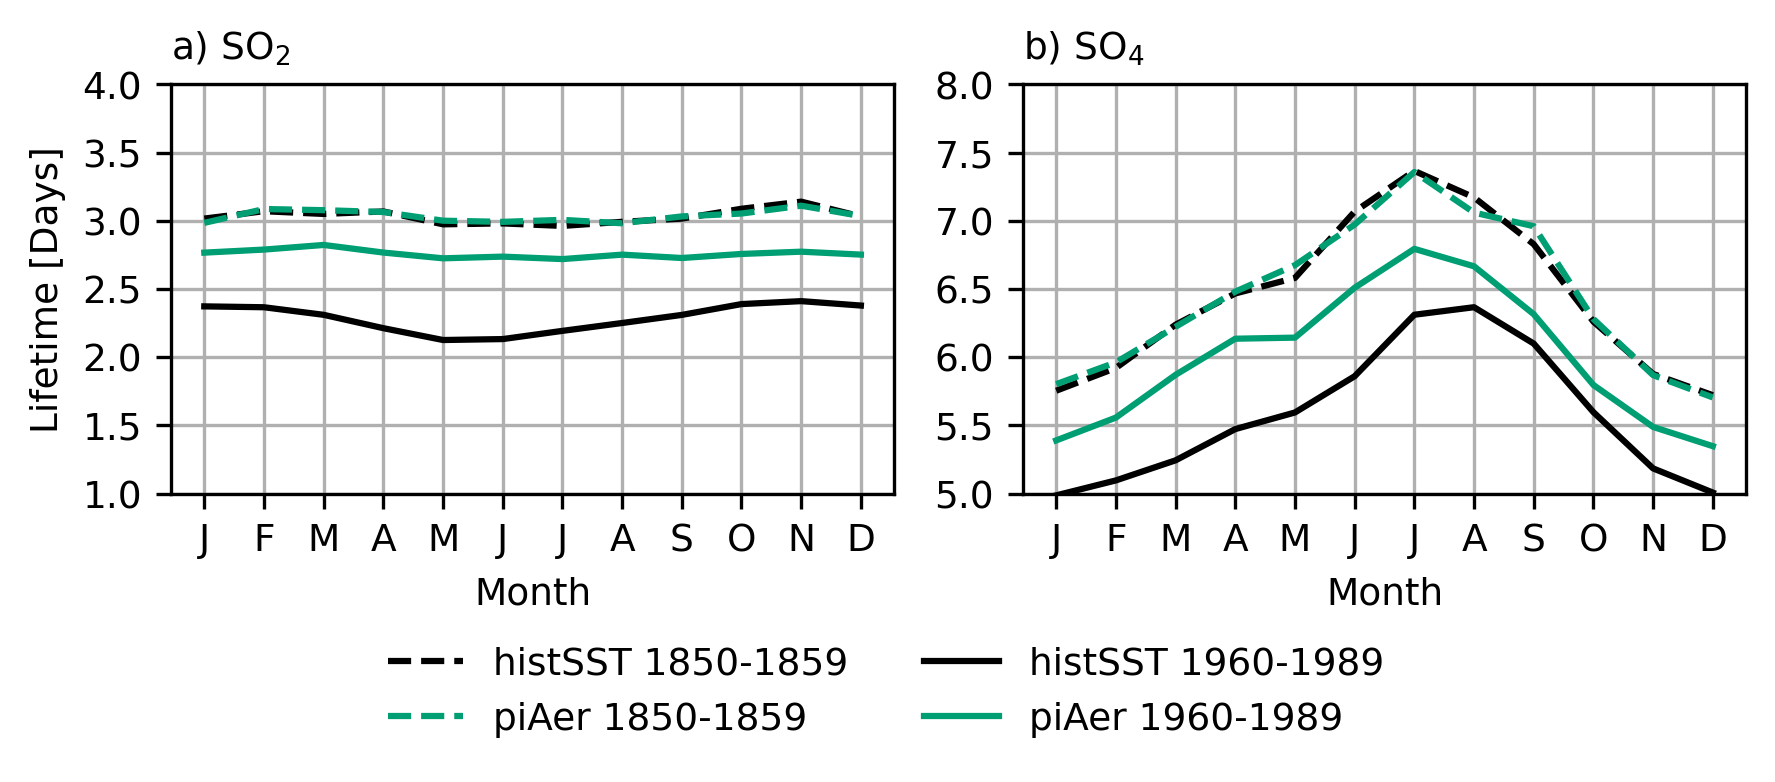
\includegraphics{Chapter4/Figs/lifetime_pothole.png}
    \caption[\ce{SO2} and \ce{SO4} lifetime by season between 1980 and 1989]{\ce{SO2} and \ce{SO4} lifetime by season between 1850--1859 and 1960--1989 from \histsst{} and \sstpiaer{}}
    \label{fig:ch4:seasonal-s-lifetime}
\end{figure}


Variation in loss mechanism modulates \ce{SO2} and \ce{SO4} lifetimes. Figure \ref{fig:ch4:seasonal-s-lifetime} shows a global mean lifetime of \ce{SO2} and \ce{SO4} for two time periods, 1850--1859 and 1960--1989, aggregated by month. When \ce{SO2} emissions are at the 1850 level, \ce{SO2} lifetimes show a slight variation across seasons, as seen in both \sstpiaer{} trends (solid and dashed green lines) and \histsst{} (dashed black line) in the 1850s. Whether this slight variation is due to an additional 0.75 \unit{Tg(S)~yr^{-1}} of emission in winter (Figure \ref{fig:app1:seasonal-emiso2-1850}) or from the variation in loss processes is inconclusive. 

The higher oxidants in the atmosphere decrease the \ce{SO2} lifetime by increasing oxidation, as seen in Chapter \ref{ch3:title}. The average \ce{SO2} lifetime decreases from 3 days to 2.75 days when oxidant level increases in the 1980s even when \ce{SO2} emissions are constrained at the 1850s level as shown by the \sstpiaer{} simulation (dashed green line versus solid green line). \ce{SO2} emissions in the 1980s decreased its mean lifetime further by 0.75 days and exacerbated the seasonal variation compared to the 1850s. The lowest \ce{SO2} lifetime is observed in May and June of the pothole period, approaching 2.0 days from the original 3.0 days in the 1850s. It could be said that \ce{SO2} emission increase at the surface drives the lifetime down. 

\ce{SO4} aerosol lifetime shows a greater variation across the season, even in the 1850s, with a shorter lifetime in winter at 5.7 days and a longer lifetime in summer at 7.3 days, showing a difference of 1.5 days between seasons. \ce{SO4} production mainly comes from \ce{SO2} oxidation which is higher during summer months (at 30 \unit{Tg(S)~yr^{-1}} compared to 20 \unit{Tg(S)~yr^{-1}} in winter; Figure \ref{fig:ch4:so2-loss}). While \ce{SO4} wet deposition increases in summer, the rate of increase is lower than production (an increase of 5 \unit{Tg(S)~yr^{-1}} between winter and summer), resulting in a higher burden and longer lifetime. 


Regarding the model performance against observations, the simulated surface \ce{SO2} and \ce{SO4} concentrations were evaluated against ground-based measurement networks in the USA and Europe by \citet{hardacreEvaluationSO2SO422021}. In polluted areas, UKESM1 overpredicts surface \ce{SO2} by a factor of 3 while underpredicts surface \ce{SO4} by 25--35\%. The mean surface \ce{SO2} concentration is overestimated, especially in summer for the 33 Eastern American ground observation sites for the period 1987--2014 \citep{hardacreEvaluationSO2SO422021}. This hints towards a better removal process for the model. 


The updated UKESM1 with modified \ce{SO2} dry deposition scheme, called UKESM1.1, has a lower surface \ce{SO2} concentration, but this exacerbates the underprediction of \ce{SO4} \citep{mulcahyUKESM1DevelopmentEvaluation2022}. This points towards the possibility that the model may need further compensation for the sulfur cycle and an increase in chemical oxidation of \ce{SO2} to convert \ce{SO2} in \ce{SO4} and potentially too large dry deposition \citep{mulcahyUKESM1DevelopmentEvaluation2022}.

% Comment on the seasonal cycle of sulfate
Overall, this section shows that seasonal changes in oxidants, cloud fractions and depositions significantly affect the fate of \ce{SO2}. \ce{SO2} emitted in summer has a greater chance of being oxidised, especially by OH, forming new \ce{SO4} aerosol particles and affecting the climate. On the other hand, \ce{SO2} emitted in winter persists in the atmosphere as a more significant burden for a longer time and can potentially be air pollutants affecting the local population and the environment. 


\subsection{Seasonal cycle of aerosol properties due to aerosol precursors}

\ce{SO2} oxidation and \ce{SO4} aerosol formation are coupled in UKESM1. Aerosol mass and number are independently diagnosed, allowing us to examine the variation in aerosol properties and size distribution due to oxidation changes. We observed more gas-phase oxidation in the boreal summer in the previous section. This section examines the aerosol properties that result from oxidation in different seasons.


\begin{figure}
    \centering
    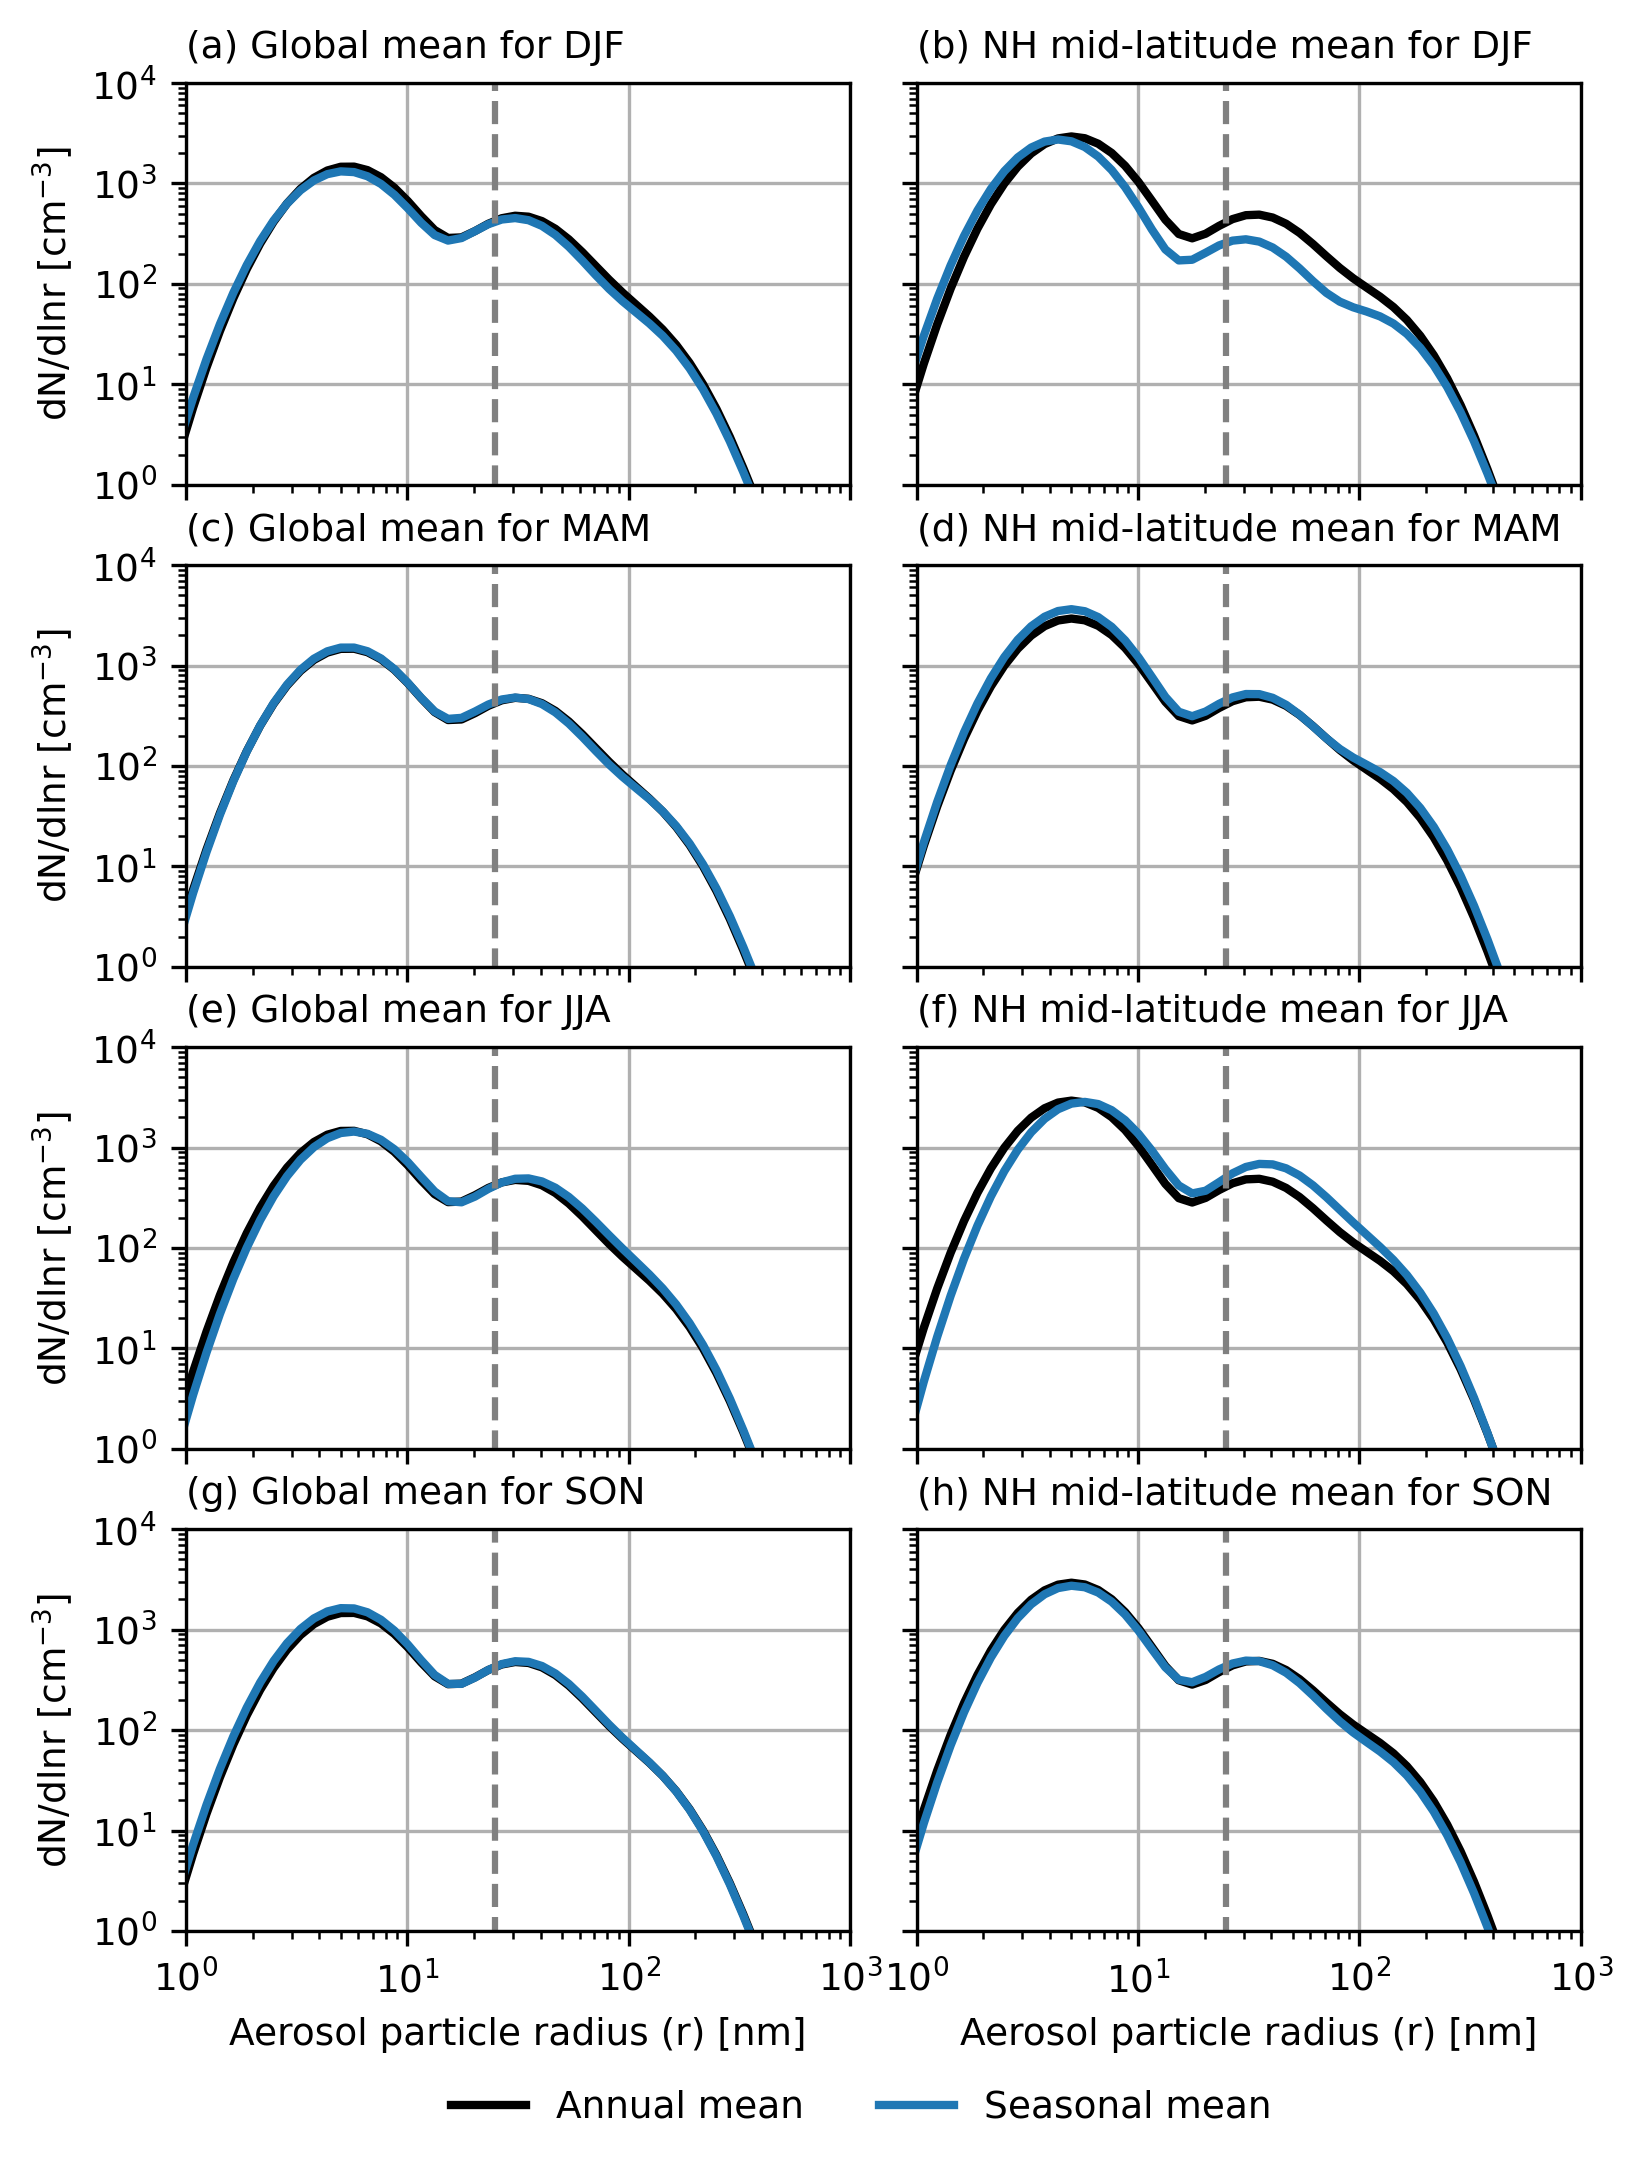
\includegraphics{Chapter4/Figs/seasonal_aerosol_size_dist_1980.png}
    \caption[Mean aerosol size distribution from the surface up to 10 km between 1980 and 1989 aggregated by seasons]{Mean aerosol size distribution from the surface up to 10 km between 1980 and 1989 aggregated by seasons. The black solid lines denote the domain annual mean. The blue lines denote the respective seasonal mean for each panel. The first column (sub-figure a, c, e, and g) shows the global mean aerosol size distribution. The second column (sub-figure b, d, f, and h) shows the mean between 30--60\textdegree N. The dashed vertical line indicates an aerosol radius of 25 nm, defined as N50 or aerosol with a diameter above 50 nm.}
    \label{fig:ch4:seasonal-aerosol-size}
\end{figure}


Figure \ref{fig:ch4:seasonal-aerosol-size} shows the variation in aerosol size distribution across the four seasons and a reference annual mean in black lines. The plots cover all aerosol components with aerosol size distribution up to accumulation mode aerosol ($\bar{r} = 1000$ \unit{\nano\metre} or $\bar{D} < 2000$ \unit{\nano\metre}) as coarse mode aerosol number concentration is negligible due to its low concentration. In the boreal summer months, June, July and August (JJA), the global mean aerosol size distribution shows minor changes to global mean aerosol size distribution (left columns) in all seasons. However, the changes are more observable in the northern hemisphere mid-latitude (30\textdegree--60\textdegree N; right column). The aerosol size distribution in winter (December, January and February; DJF) is lower than the annual mean, especially for aerosol with a radius greater than 25 \unit{\nano\metre} or diameter above 50 \unit{\nano\metre} (N50), which acts as cloud condensation nuclei. The opposite is true for the same region over summer (June, July and August; JJA) when we have observed more gas-phase oxidation.


The \ce{SO2} oxidation pathways could explain the shift in aerosol size distribution in summer and winter and how the model simulates aerosol processes. In UKESM1, \ce{SO2} gas-phase reaction produces \ce{H2SO4} gas, which condenses into new nucleation mode aerosol particles \citep{mannDescriptionEvaluationGLOMAPmode2010}. On the other hand, \ce{SO2} aqueous-phase reactions add \ce{SO4} mass onto the existing aerosols in accumulation and coarse mode without forming new particles. As we saw from the previous section, there is more \ce{SO2 + OH} reaction during summer. This additional aerosol particle production increases the accumulation mode (peaks at a 30 nm radius) aerosol number in summer. 


\begin{figure}
    \centering
    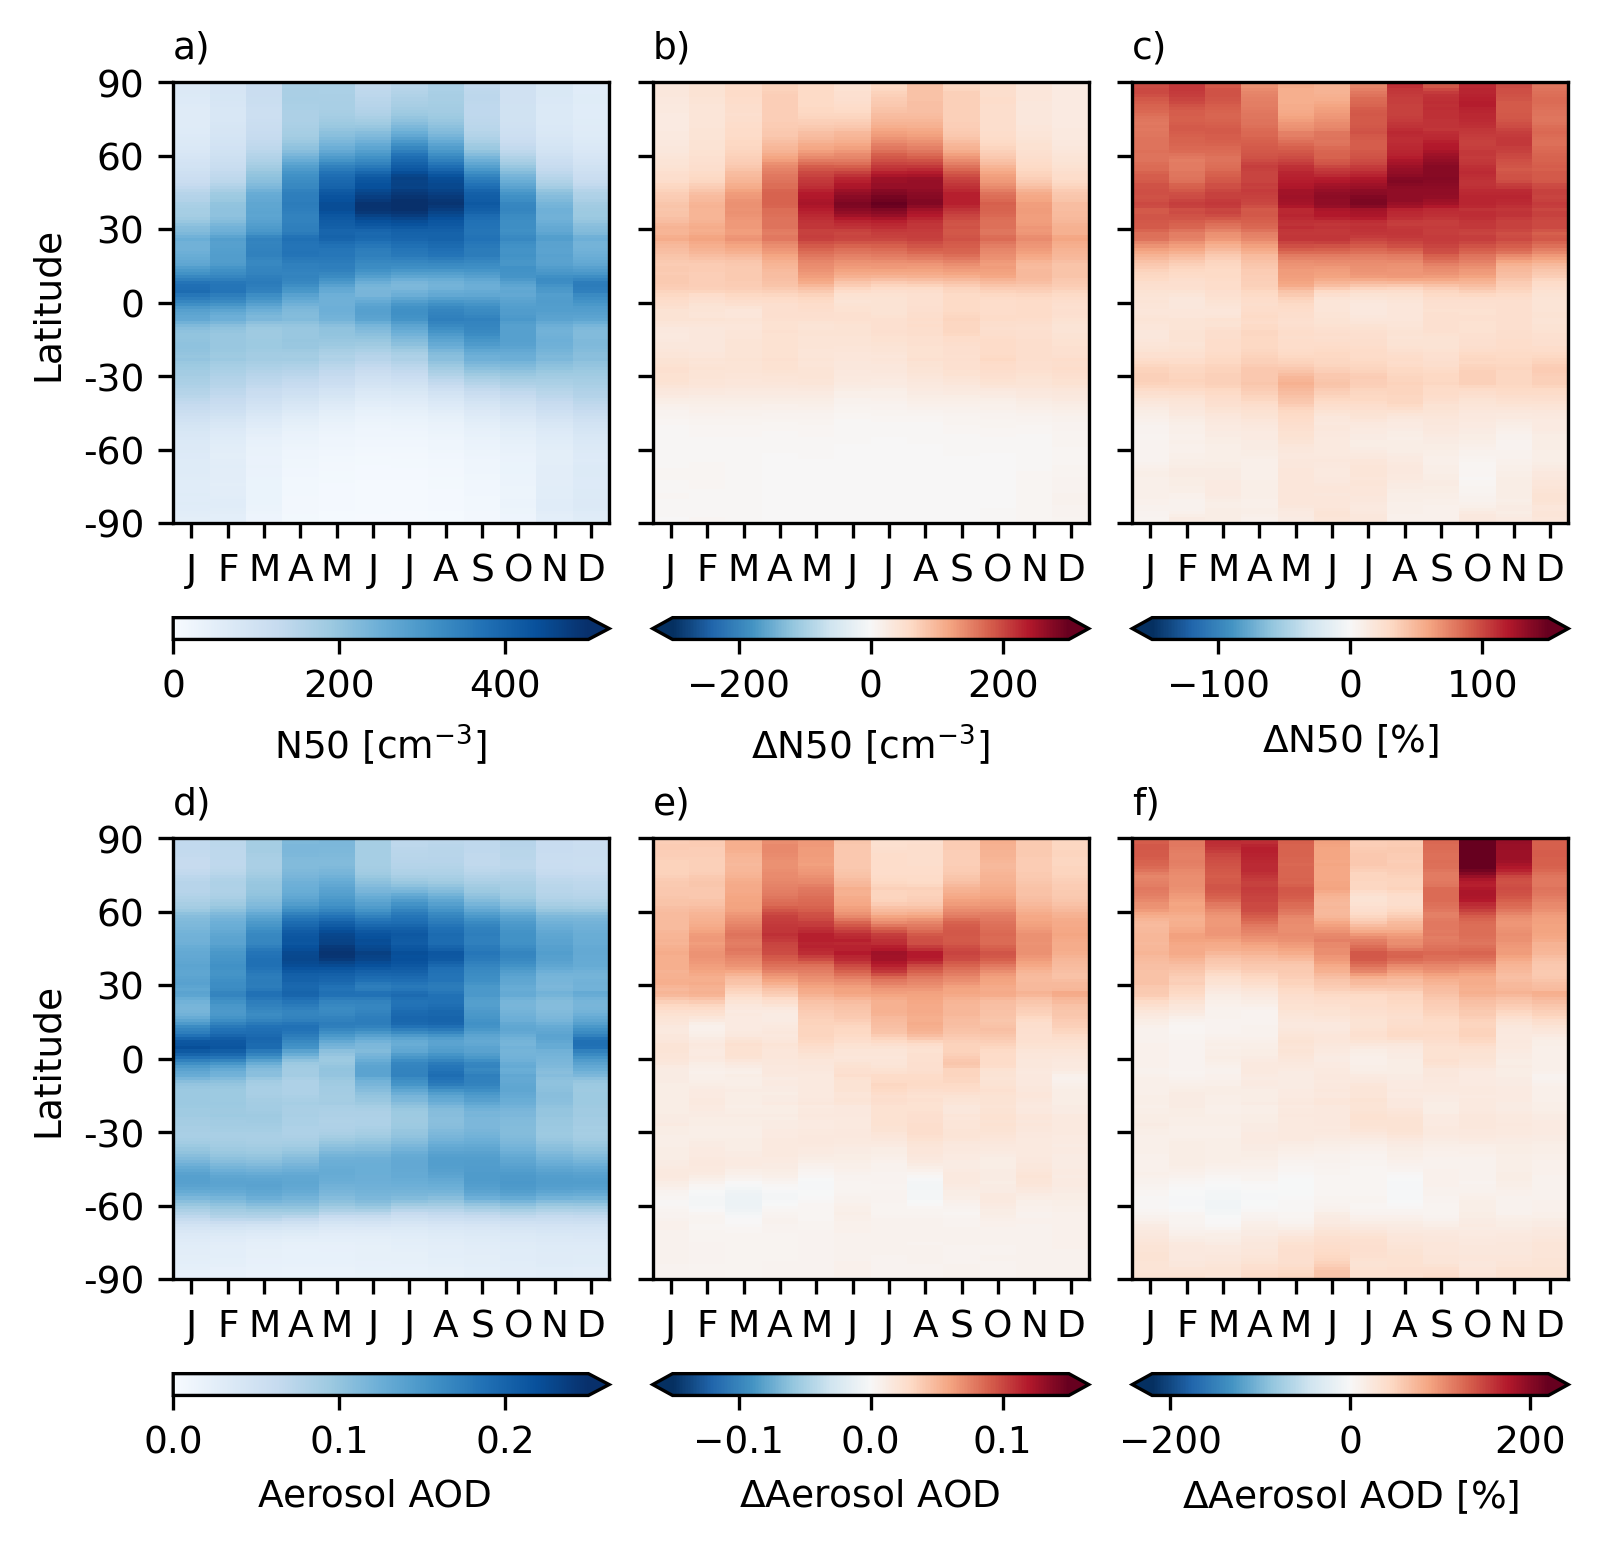
\includegraphics{Chapter4/Figs/seasonal_aerosol_props_1980.png}
    \caption[Mean AOD at 550 nm and N50 between 1980 and 1989 as a function of months and latitude due to aerosol precursor emissions]{mean (a--c) number concentration of aerosol with a diameter greater than 50 nm (N50) from the surface up to 10 km and (d--f) AOD at 550 nm between 1980 and 1980 as a function of months and latitude. The first column is the absolute value, and the second and third columns are the changes in aerosol properties due to aerosol precursor emissions (\histsst{} minus \sstpiaer{}) in absolute and relative terms, respectively.}
    \label{fig:ch4:seasonal-aerosol-props}
\end{figure}


Aerosol properties such as AOD and aerosol number concentration, especially for N50, are quantities that link to radiative adjustment due to aerosols. Figure \ref{fig:ch4:seasonal-aerosol-props} shows aerosol macroscopic properties, including the AOD and N50 concentration and the changes due to aerosol precursor emissions. Aerosol precursor emission adds more than 200 \unit{cm^{-3}} or more than 150\% to N50 between June and August in the Northern Hemisphere. Although there are more significant \ce{SO2} emissions in the same region in winter, this translates into lesser growth in N50 of approximately 50\%.


Aerosol optical depth (AOD) quantifies the absorption or scattering of light by the aerosol layer in the atmosphere, providing a measure of aerosols' columnar concentration in the atmosphere. Aerosol AOD shows a slightly different seasonal trend from N50. While there is an increase in AOD in summer when more oxidation is observed, the seasonal trend agrees better with the \ce{SO4} burden in Figure \ref{fig:ch4:seasonal-s-burden}. 


Studies show that UKESM1 and GLOMAP-mode, its aerosol component, are skilful in predicting sulfate aerosol trends between 1980 and 2009, with the tendency to underpredict sulfate aerosol concentration in Europe and East Asia compared to observations \citep{mannDescriptionEvaluationGLOMAPmode2010, mulcahyDescriptionEvaluationAerosol2020}.  The model well predicts the spatial distribution of sulfate aerosol distribution but consistently underpredicts the absolute values for all years, although it is within the observed variability. The model also underpredicts East Asian observations to a greater degree than GC3.1, a model with the same physical atmosphere-ocean and aerosol component but a lower level of interaction within the Earth system. With the updated dry deposition scheme in UKESM1.1, the model further underpredicts sulfate aerosol loading \citep{hardacreEvaluationSO2SO422021}. As discussed in the next section, even with underpredicted sulfate aerosol, the model shows a substantial change in cloud properties compared to other Earth system models. 


\subsection{Seasonal cycle of cloud properties}

Aerosol acts as cloud condensation nuclei, allowing water vapour to condense at lower temperatures than homogeneous nucleation. Thus, the change in aerosol number and size modifies cloud properties \citep[e.g. ][]{rosenfeldGlobalObservationsAerosolcloudprecipitationclimate2014, boucherCloudsAerosols2014,persadAerosolsMustBe2022}. Aerosol in the cloud increases its albedo and lifetime, leading to weather and climate effects \citep{twomeyInfluencePollutionShortwave1977, albrechtAerosolsCloudMicrophysics1989}. This section aims to quantify the change in cloud properties due to aerosol precursor emissions in different seasons.

\begin{figure}
    \centering
    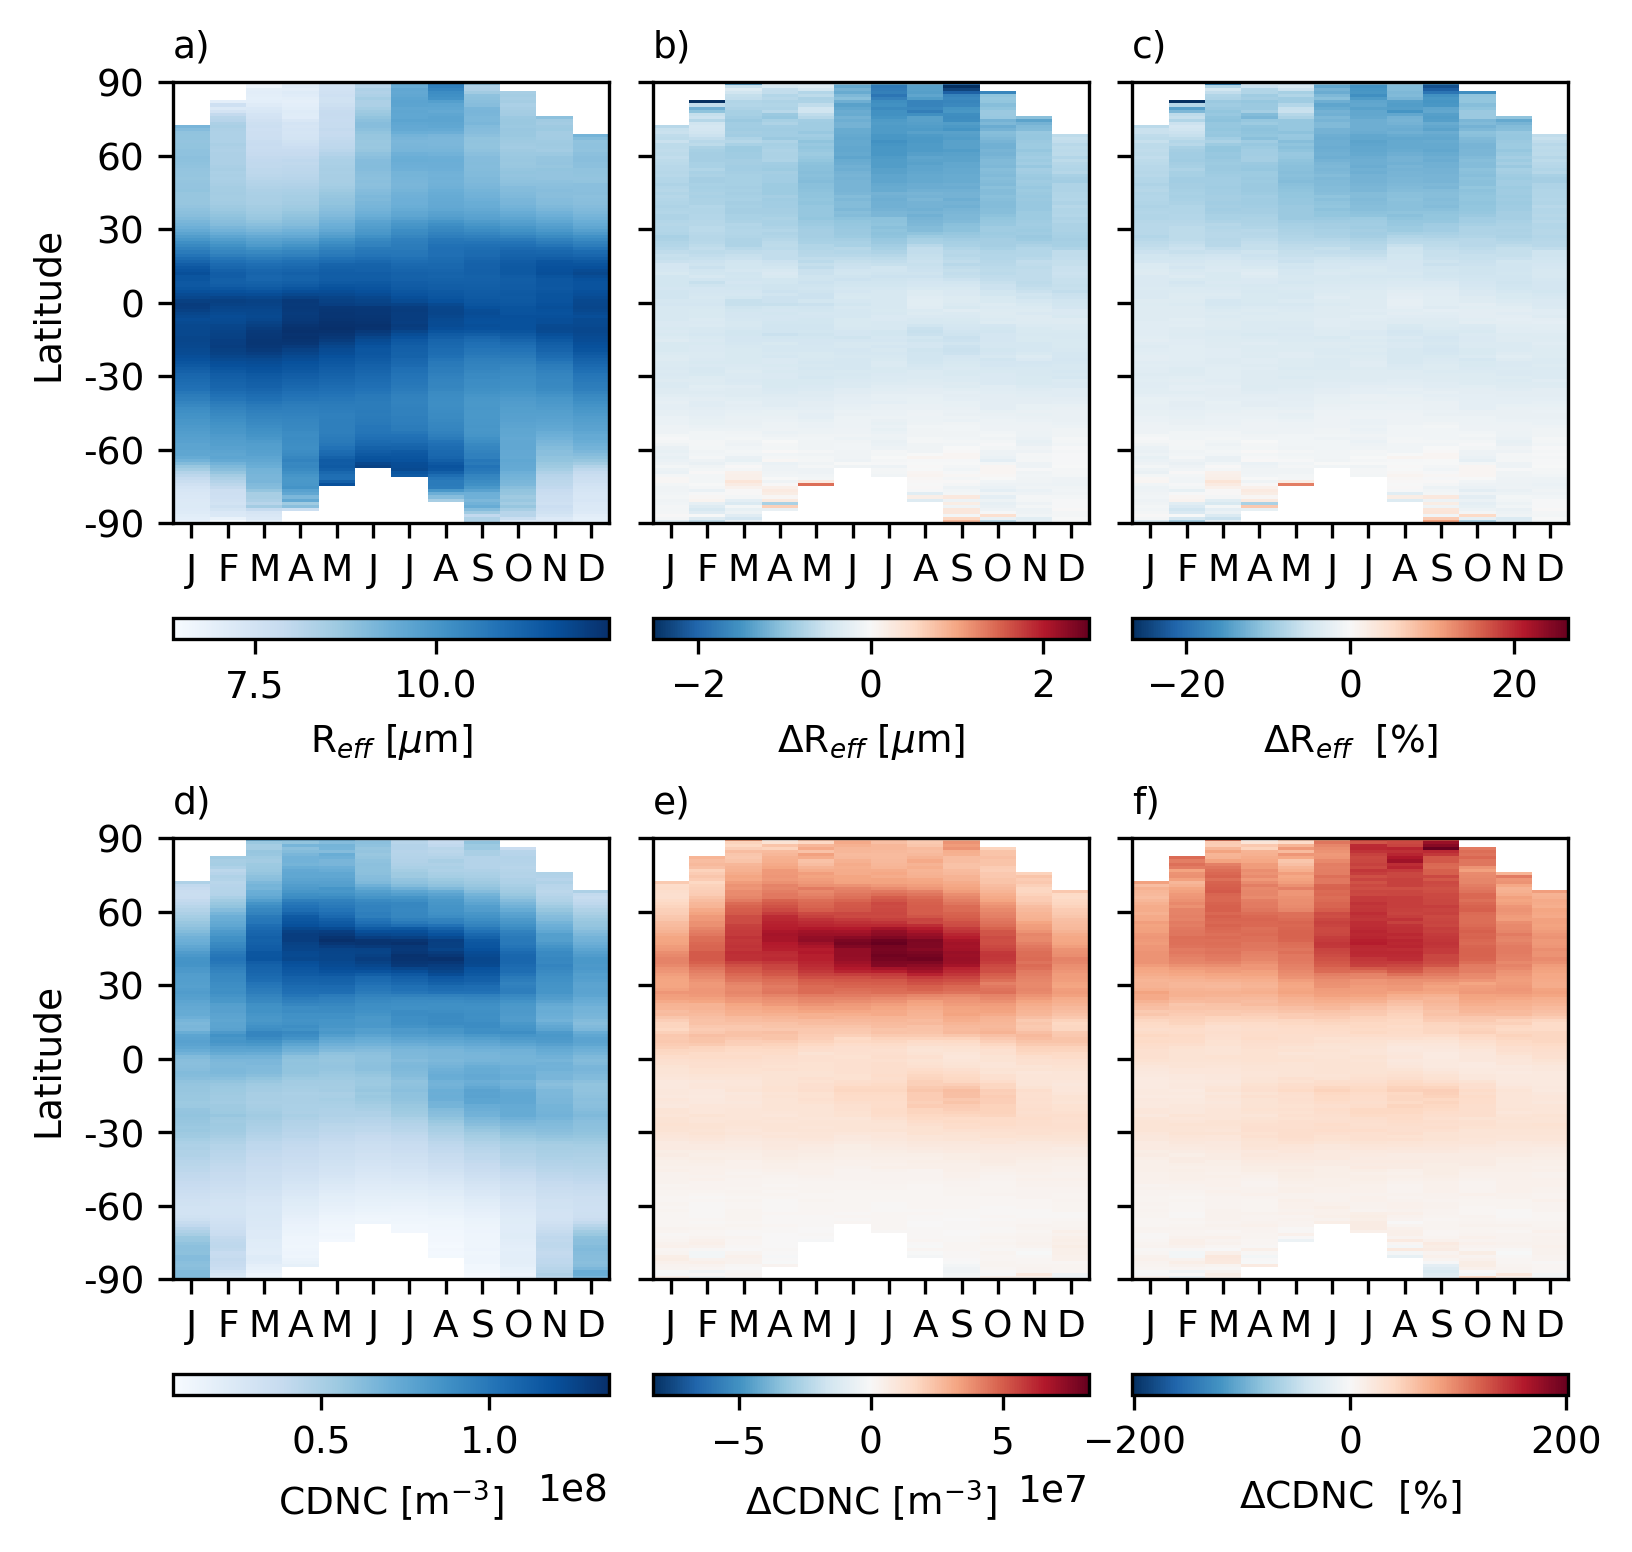
\includegraphics{Chapter4/Figs/seasonal_cloud_props1_pothole.png}
    \caption[\Reff{} and CDNC aggregated by latitude and month between 1960 and 1989]{a) shows mean \Reff{} from \histsst{} aggregated by latitude and month between 1960 and 1990 below 10 km. b-c) shows the change in \Reff{} due to aerosol precursor emissions (\histsst{} minus \sstpiaer{}) in absolute value and the percentage of change compared to \sstpiaer{}, respectively. d-f) show a similar analysis for CDNC.}
    \label{fig:ch4:seasonal-cloud-props1}
\end{figure}


Figure \ref{fig:ch4:seasonal-cloud-props1} shows the effect of aerosol precursor emissions on cloud properties. Cloud droplet effective radius, \Reff{}, at 30 to 60 \textdegree N is decreased by approximately \qty{1.5}{\micro\metre} or 10\% between June and September. The cloud droplet number concentration, CDNC, sees a more significant change at 100\% at the same month and latitude. 



\begin{figure}
    \centering
    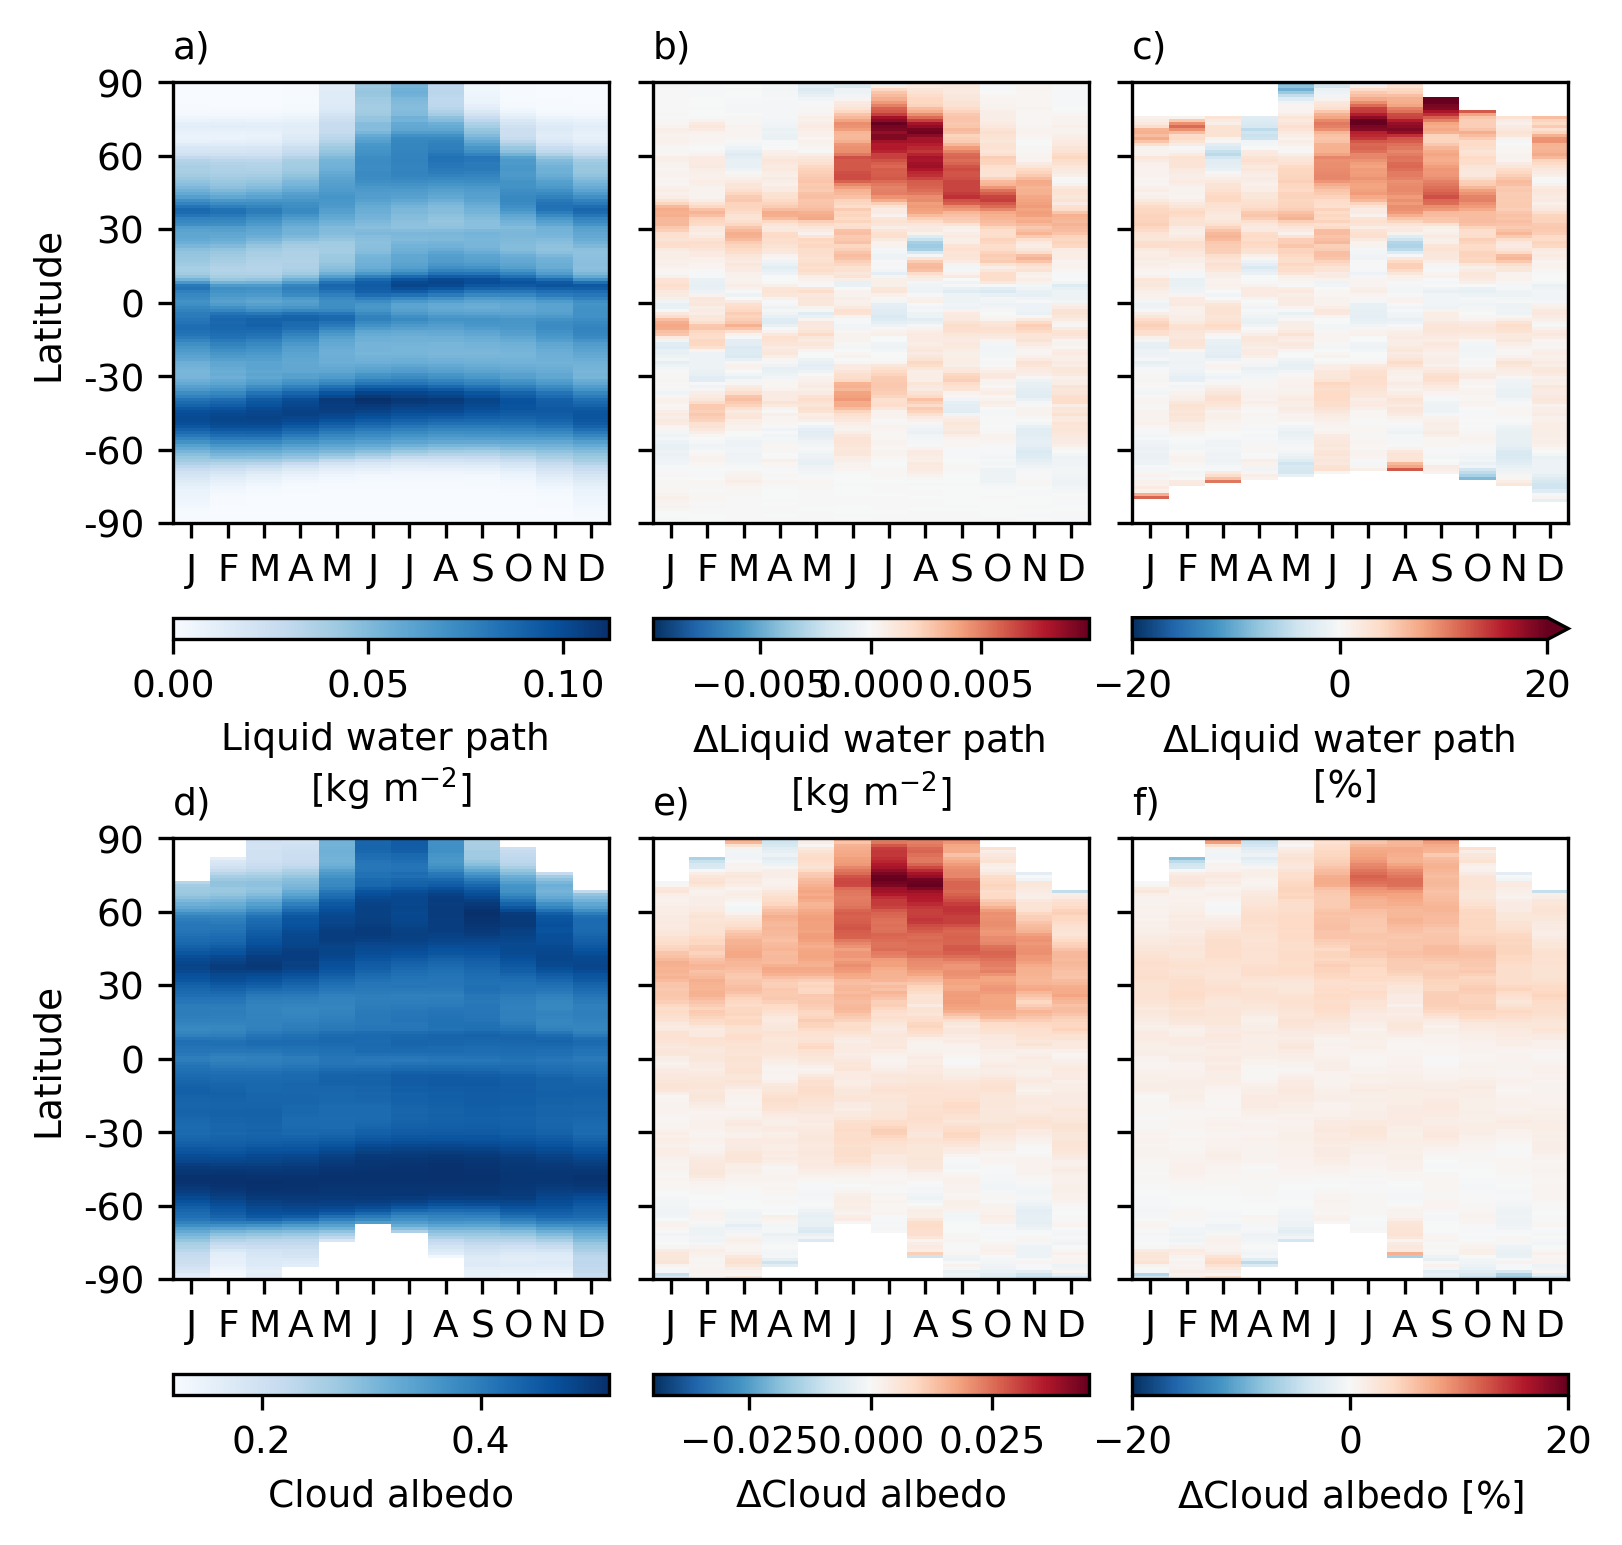
\includegraphics{Chapter4/Figs/seasonal_cloud_props2_pothole.png}
    \caption[Cloud liquid water path and albedo aggregated by latitude and month between 1960 and 1989]{a) shows mean liquid water path from \histsst{} aggregated by latitude and month between 1960 and 1990 below 10 km. b-c) shows the change in liquid water path due to aerosol precursor emissions (\histsst{} minus \sstpiaer{}) in absolute value and the percentage of change compared to \sstpiaer{}, respectively. d-f) show a similar analysis for cloud albedo.}
    \label{fig:ch4:seasonal-cloud-props2}
\end{figure}

Cloud reflectance increases as the droplet size decreases. Figure \ref{fig:ch4:seasonal-cloud-props2} shows the cloud liquid water path, the vertical integration of cloud liquid water content and cloud albedo. The liquid water path in the northern hemisphere, especially during summer, increases by 15--20\% due to aerosol precursor emissions. This results in a 10\% more reflective cloud in boreal summer. The result shows that the effect of aerosol precursors on cloud is localised and correlates to \ce{SO2} oxidation rather than emissions.

% Discuss cloud simulation in UKESM1 and any validations of this run
While the results above show substantial cloud response to aerosol precursors, most cloud properties exhibit a low bias compared to MODIS satellite measurements from March 2009 to March 2010 in the North Atlantic Ocean region \citep{grosvenorDecompositionCloudAerosol2020}. According to \citet{grosvenorDecompositionCloudAerosol2020}, the atmosphere-only version of UKESM1 can capture the cloud spatial pattern with a spatial correlation above 0.8 but consistently underestimates cloud cover and liquid water path. Low- and mid-altitude cloud fraction is lower by a normalised mean bias factor (NMBF) of -28--37\%. The high altitude cloud is the least biased at -8.5\%. In-cloud liquid water path is also underestimated with NMBF of -20\%. In contrast, cloud droplet number concentration is overestimated by 11.3\%.

\change[inline]{Add discussion on the impact of GLOMAP-mode on aerosol forcing in HadGEM3 https://acp.copernicus.org/articles/13/3027/2013/}

It is essential to note that UKESM1 has the largest change in cloud fraction from aerosol precursor emissions amongst 6 ESMs with interactive chemistry and aerosol schemes that participated in AerChemMIP \citep{zhangRoleAnthropogenicAerosols2021}. While UKESM1 underestimates cloud fraction, it also has the strongest sensitivity to aerosol loading \citep{zhangRoleAnthropogenicAerosols2021}, but model aerosol sensitivity does not predict pothole cooling. More comparison is needed between models to diagnose the underpinning aerosol and process that leads to pothole cooling. 


\subsection{Seasonal cycle of ERF due to aerosol precursors}


I have shown that \ce{SO2} emissions increase during boreal winter with more energy demands, but aerosol formation does not follow seasonal emission trends. Instead, new \ce{SO4} aerosol particles form when more OH is present for gas-phase oxidation, leading to more aerosol number concentration and brighter clouds in boreal summer. This section discusses the seasonal trend in aerosol-radiation interaction and establishes the correlation between ERF and oxidation processes. Finally, I show quantitatively that the emission timing is responsible for more aerosol formation in summer using the concept of specific ERF.


\begin{figure}
    \centering
    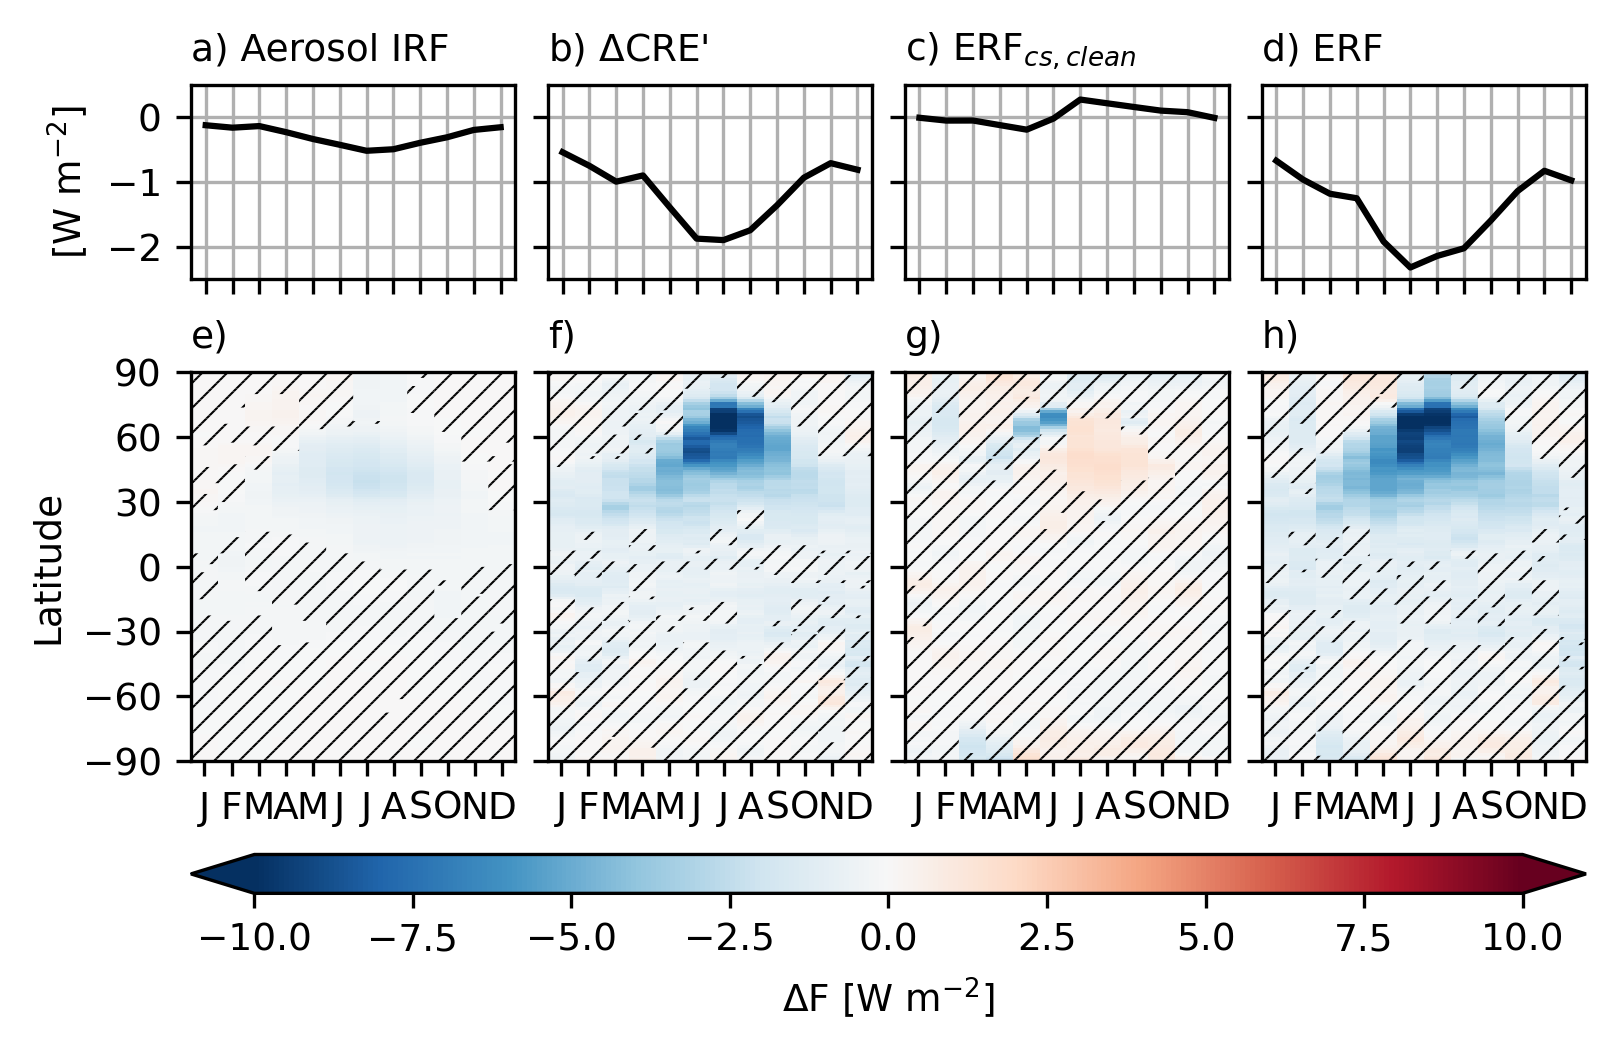
\includegraphics{Chapter4/Figs/latitudinal_erf_sstpiaer-histsst_pothole.png}
    \caption[ERF due to aerosol precursor emissions between 1960--1989 aggregated by month and latitude]{ERF due to aerosol precursor emissions between 1960--1989 aggregated by month and latitude. Each data point is averaged longitudinally, giving 10 data points for each month and latitude. Hatch denotes points where the difference between \histsst{} and \sstpiaer{} is insignificant (p$\leq$0.05).}
    \label{fig:ch4:seasonal-erf}
\end{figure}


Contrary to the assumed correlation between emissions and ERF. Figure \ref{fig:ch4:seasonal-erf} shows a strong seasonal cycle with a high negative in the boreal summer between 1960 and 1989, when \ce{SO2} emissions are lowest annually. Aerosols have less radiative impacts in boreal winter above latitude 45\textdegree N even though \ce{SO2} emission is the strongest in winter. 


% Discuss the ERF from different cloud adjustments
Aerosol radiative effects act mainly in the shortwave. The atmosphere-only version of UKESM1 shows a negative bias in low-altitude cloud fraction with -28.1\% NMBF while overestimating shortwave outgoing radiation at the top of the atmosphere by 1.7--5.8\% NMBF compared to the MODIS satellite observation in the present-day simulation \citep{grosvenorDecompositionCloudAerosol2020}. CDNC is underestimated in the northern North Atlantic Ocean region but overestimated in the southern North Atlantic Ocean by 21.5\%. However, this does not contribute substantially to the bias of outgoing shortwave radiation at the top of the atmosphere \citep{grosvenorDecompositionCloudAerosol2020}. This shows that the model predicts a radiation response from clouds over the Northern Atlantic that is too strong. Whether this correlation applies to other regions is unknown.


\begin{figure}
    \centering
    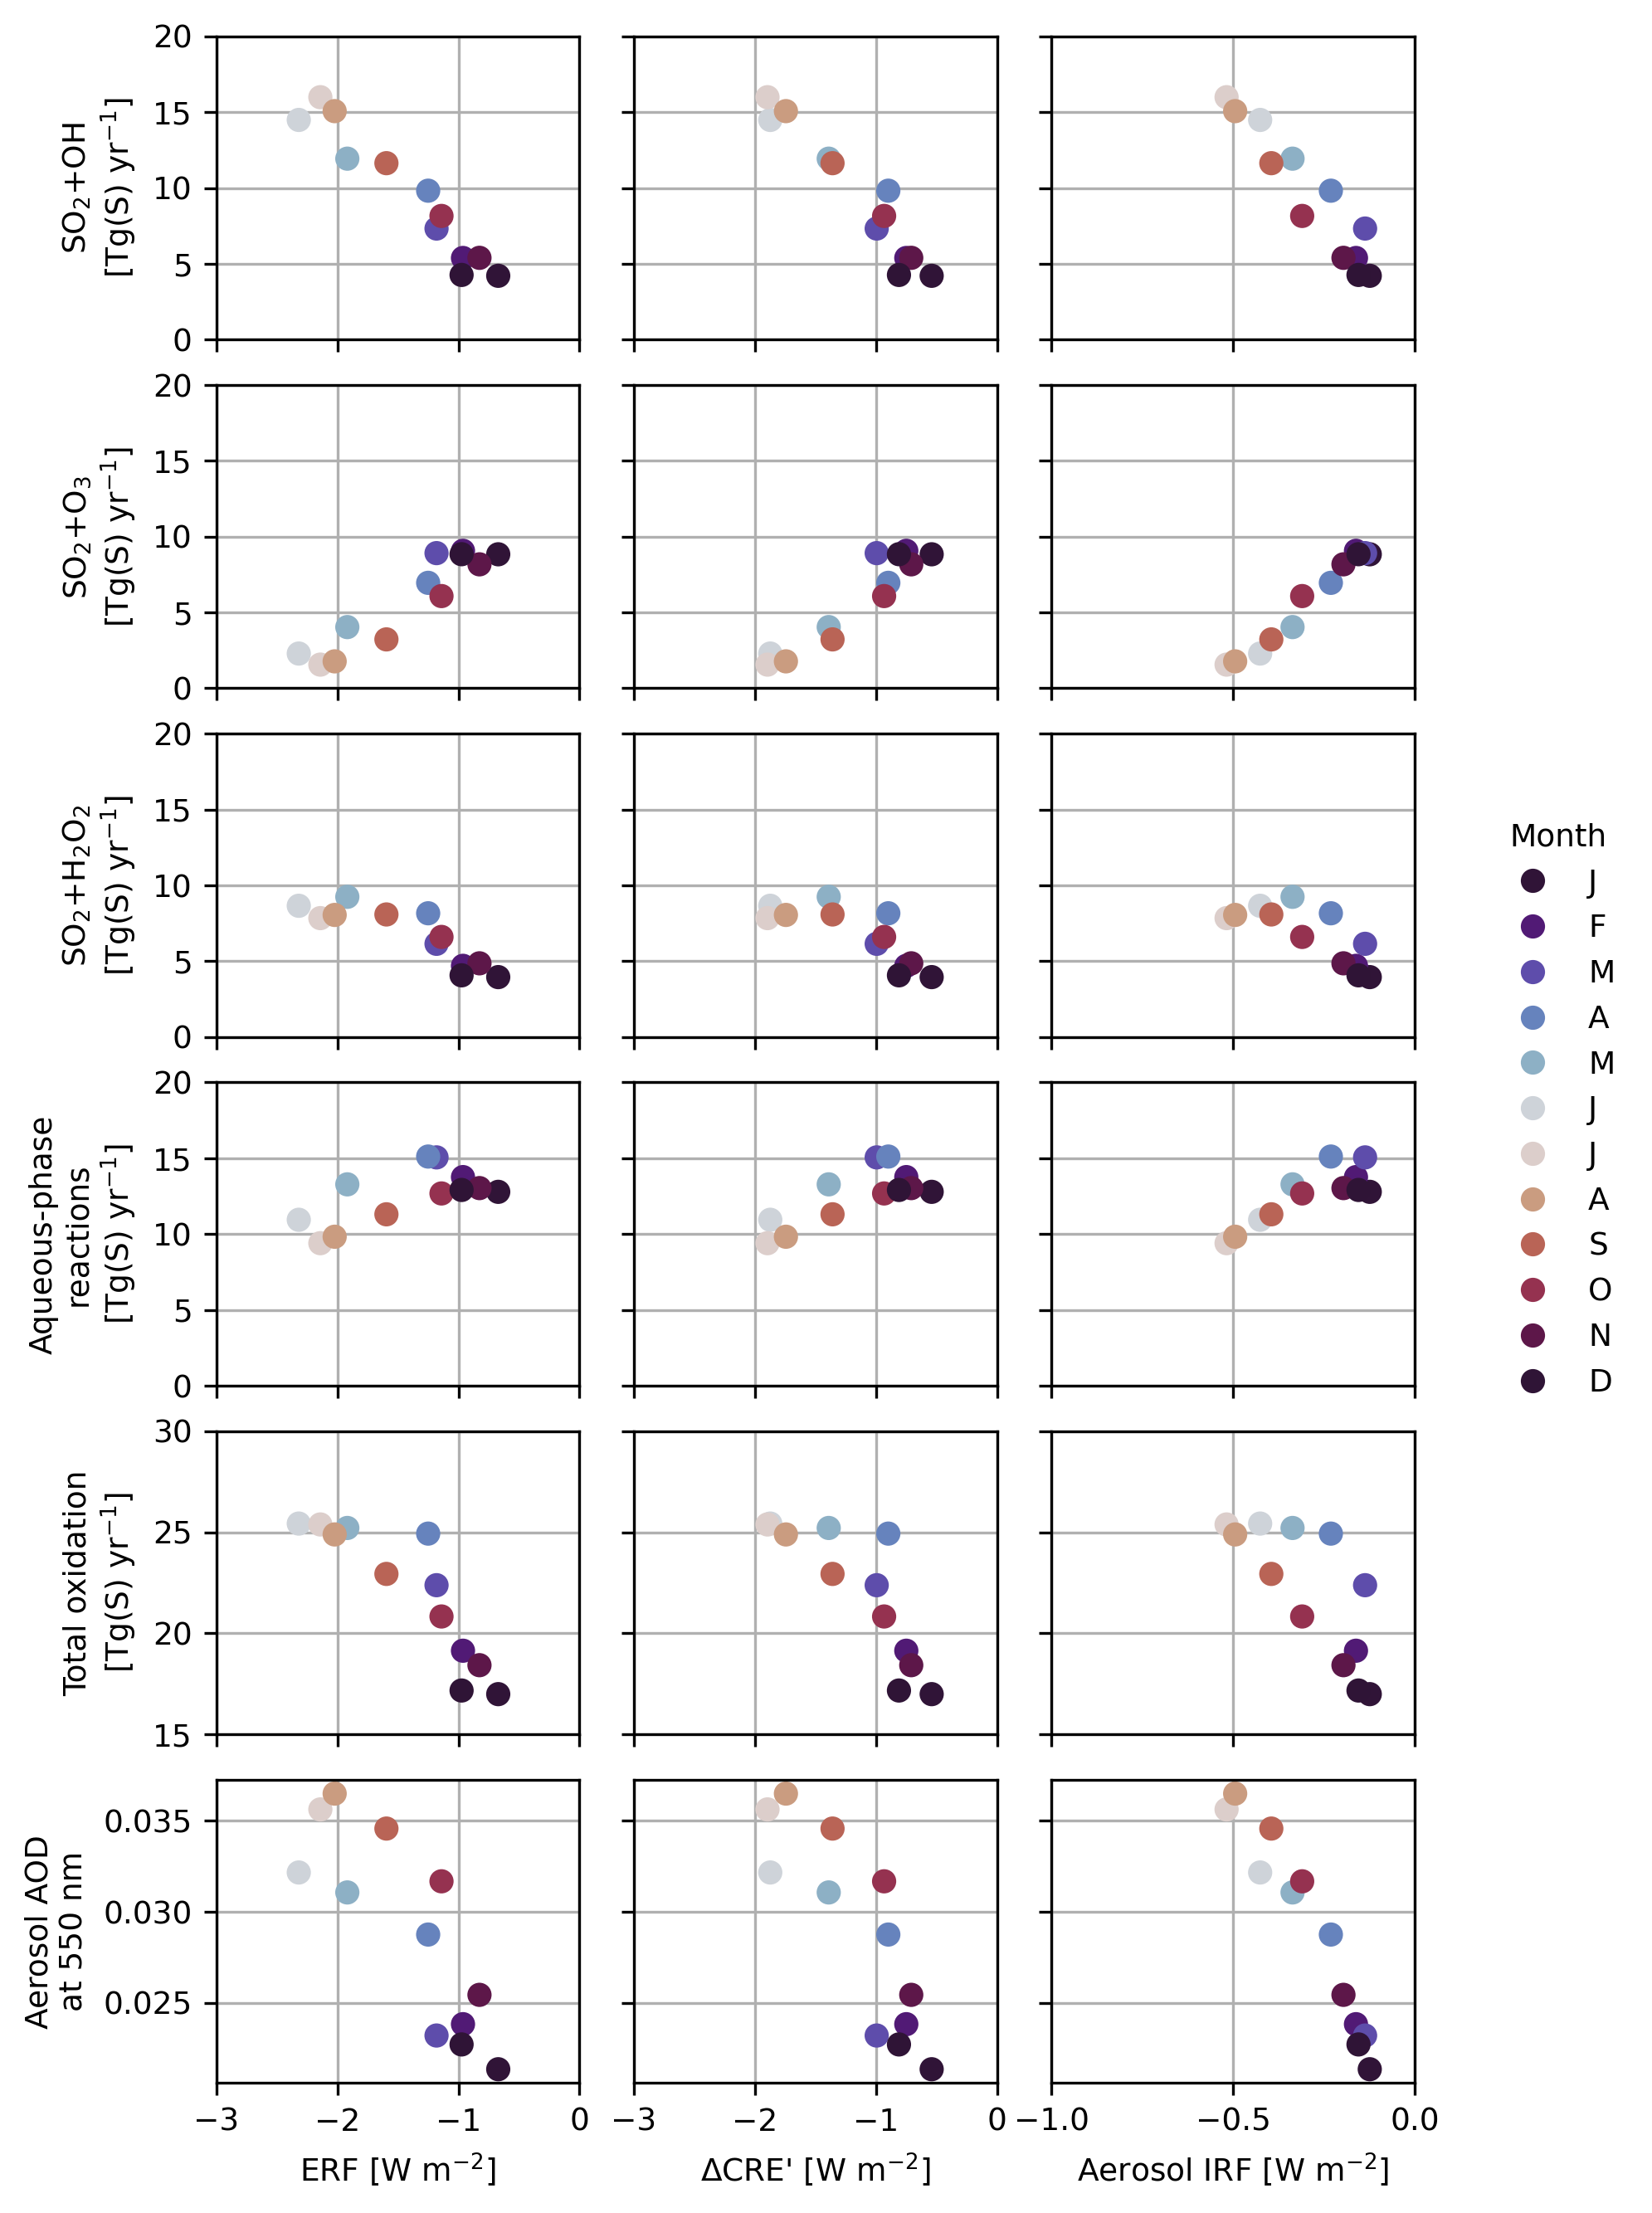
\includegraphics[width=\linewidth]{Chapter4/Figs/seasonal_oxidation_erf_corr_pothole.png}
    \caption[Correlation between \ce{SO2} oxidation tendencies and ERF between 1960 and 1989]{Correlation between \ce{SO2} oxidation tendencies and ERF between 1960 and 1989}
    \label{fig:ch4:seasonal-erf-corr}
\end{figure}

Figure \ref{fig:ch4:seasonal-erf-corr} shows the correlation between oxidation, AOD and radiative forcing. \ce{SO2 + OH} shows an inverse linear relationship with ERF, with greater oxidation tendency and more negative ERF in June--August. Neither total oxidation nor aerosol AOD correlate well with ERF. This suggests that gas-phase oxidation is a valuable parameter for this type of analysis. This plot indicates that oxidation tendencies explain ERF and not emission.


\begin{figure}
    \centering
    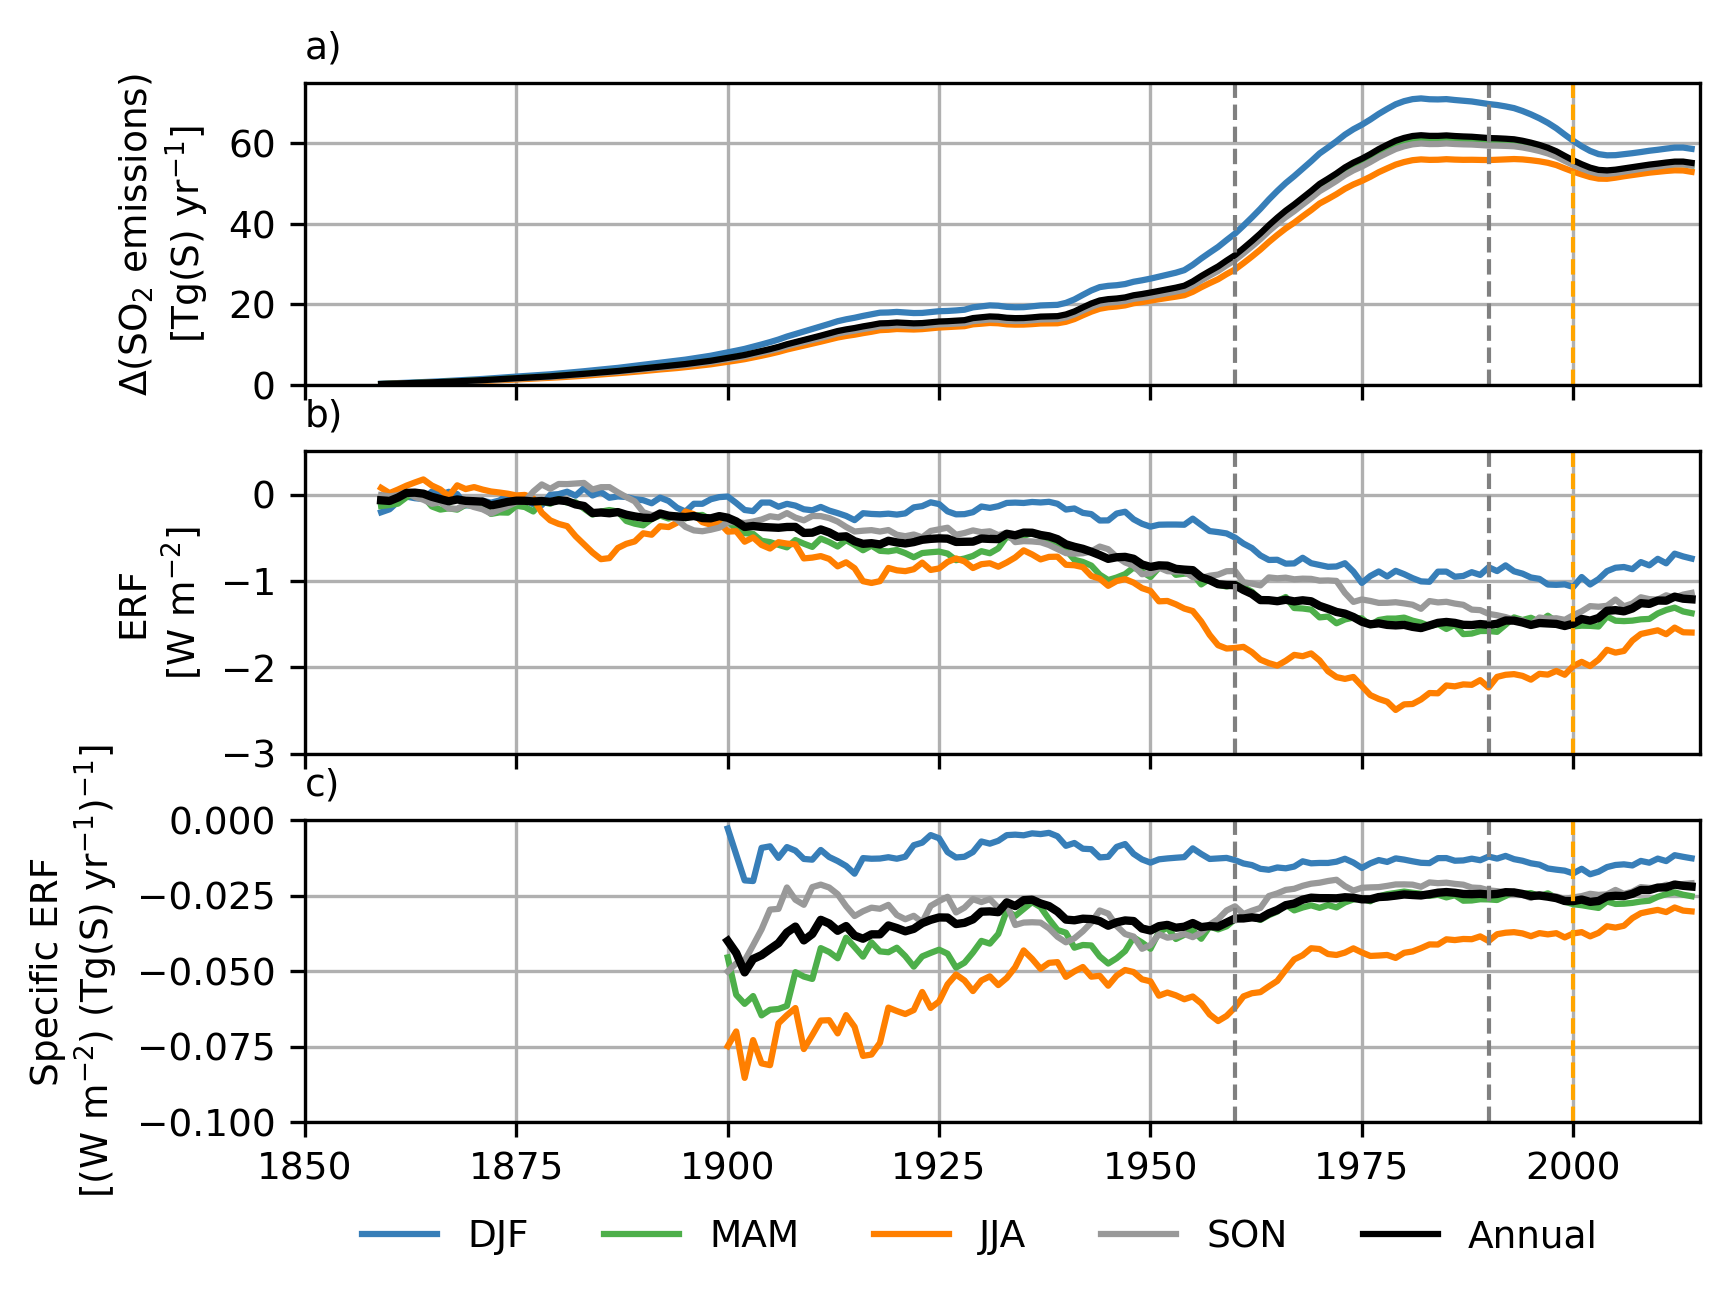
\includegraphics{Chapter4/Figs/seasonal_specific_erf.png}
    \caption[Specific ERF aggregated by seasons between 1900--2014]{Changes due to aerosol precursor emissions (i.e. \histsst{} minus \sstpiaer{}) of a) \ce{SO2} emissions, b) ERF and c) specific ERF (ERF per emitted \ce{SO2} aggregated by seasons with 10-year rolling average. Specific ERF is shown for 1900 onwards due to high noise from a small denominator. }
    \label{fig:ch4:specific-erf}
\end{figure}

Due to the nature of the available oxidants, \ce{SO2} emitted in summer has a stronger potential to impact the climate, as shown in Figure \ref{fig:ch4:specific-erf}. Specific ERF is the ERF per unit of \ce{SO2} emissions, following work by \citet{bellouinRegionalSeasonalRadiative2016}. During the pothole period, each teragram of sulfur emission contributes 4 times more cooling than the same amount emitted in winter (0.05 compared to 0.125 \unit{(W~m^{-2})~(Tg(S)~yr^{-1})^{-1})}. Specific ERF in autumn (SON) and winter (DJF) show less variation compared to summer, averaging at 0.125 \unit{(W~m^{-2})~(Tg(S)~yr^{-1})}. In contrast, specific ERF in Summer (JJA) decreases over time but is still at least 2 times greater than in winter.

% Note on Bellouin's 2016 work on specific RF. 
A previous study shows aerosol ERF is stronger in summer, especially when emissions are from Europe \citep{bellouinRegionalSeasonalRadiative2016}. Moreover, the specific RF from HadGEM3, a lower complexity model which predates UKESM1, is the most significant specific RF from \ce{SO2} emission in all models included in \citet{bellouinRegionalSeasonalRadiative2016}'s study. 


% there is substantial cooling from sulfate aerosol in summer, would it impact global mean surface air temperature?
It is now established that aerosols' impact on radiation is stronger in summer. Work done in this Chapter has contributed to understanding the observed behaviour in aerosol ERF.


\subsection{Surface air temperature anomaly and connection to aerosol radiative forcing}
\label{ch4:sec:seasonal-tas}

Aerosol-radiation interaction enhances the scattering of outgoing shortwave radiation, resulting in a negative ERF, which is shown to be stronger during the summer close to the emission region. There is evidence of aerosol impact on regional temperature change in diurnal time scale across seasons \citep[e.g. ][]{hanMechanismsSeasonalDifferences2020}. However, contrasting evidence exists on a global and longer temporal span, especially over the ocean. 

Aerosol's effect is local in the shorter and more regional scale. Anthropogenic aerosols indirectly increase surface temperature and decrease the diurnal temperature range in East Asia by reducing shortwave solar radiation and rising cloudiness and cloud liquid water \citep{huangImpactAerosolIndirect2006}. Aerosols reduce the global terrestrial mean diurnal temperature range by 0.47 K, with almost half the contribution coming from aerosols of anthropogenic origin \citep{chakrabortyLandCoverRegulates2019}. Aerosol causes changes in local air temperature, as observed in the urban heat island effect on a short time scale and regional scale \citep{hanMechanismsSeasonalDifferences2020}. % Explain urban heat island. 
Aerosols reduce urban heat island intensity in summer by cooling down surface temperature more strongly in urban areas than in rural areas but increase it in winter by weakening heat transport and expanding the planetary-boundary-layer stability.

While aerosol affects radiation budget locally and temporally on a short time scale, change in surface temperature does not have a simple localised or linear response to aerosol perturbation. Modelling studies show that sea surface temperature change due to aerosol shows a similar pattern to homogeneous forcing, i.e. greenhouse gases \citep{xieSimilarSpatialPatterns2013,kasoarSimilarSpatialPatterns2018}. Aerosols from different industrial regions (North America, Europe, East and South Asia) cause significant cooling across the hemisphere, showing a consistent spatial pattern of temperature changes regardless of the emission source \citep{kasoarSimilarSpatialPatterns2018, lewinschalLocalRemoteTemperature2019}.  


Acknowledging the multifaceted challenges, this section explores simulated surface air and sea temperature and compares them to observations to diagnose its possible connection to anomalous or pothole cooling observed between 1960 and 1980. 


\begin{figure}
    \centering
    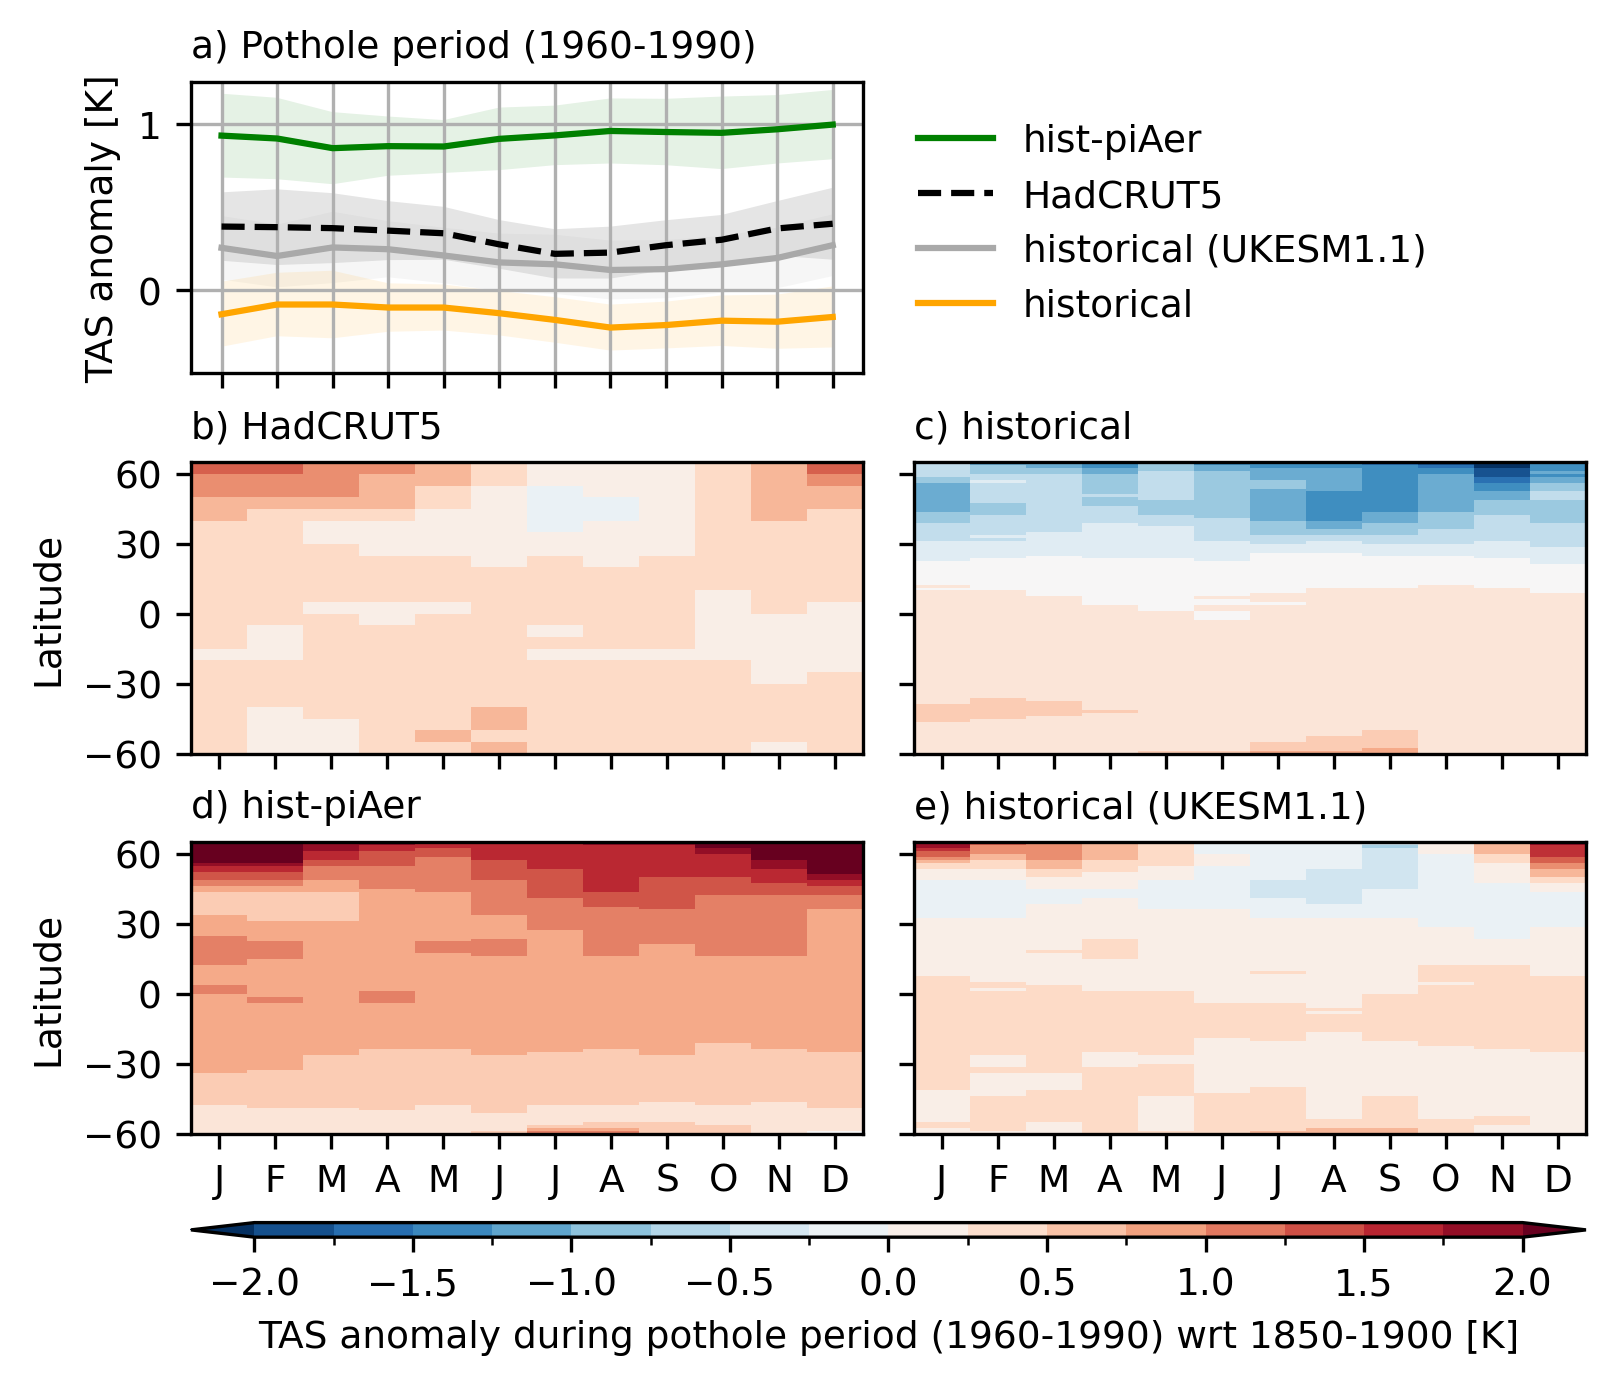
\includegraphics{Chapter4/Figs/TAS_anomaly_pothole.png}
    \caption[Surface air anomaly from HadCRUT5, UKESM1 and UKESM1.1 between 1960 and 1989]{a) mean surface air temperature anomaly between 1960--1989 with respect to 1850--1899 averaged over latitude 60\textdegree S and 65\textdegree N aggregated by month. b) surface air temperature anomaly from HadCRUT5 adjusted to 1850--1899. c-e) shows surface air temperature from UKESM1 c) \hist{} and d) \histpiaer{} simulation. d) is the same as c but from UKESM1.1. }
    \label{fig:ch4:seasonal-tas-anomaly-pothole}
\end{figure}

Figure \ref{fig:ch4:seasonal-tas-anomaly-pothole} shows the surface air temperature (TAS) from observation and model. HadCRUT5 shows a seasonal trend in TAS with the lowest temperature observed between June and September between Latitude 30 and 60 \textdegree N. The UKESM1 captures this trend but underestimates TAS globally. In contrast, the TAS anomaly in \histpiaer{} shows a different seasonal trend with the lowest anomaly in March. This shows that aerosol precursor controls the seasonal trend in TAS. 


\begin{figure}
    \centering
    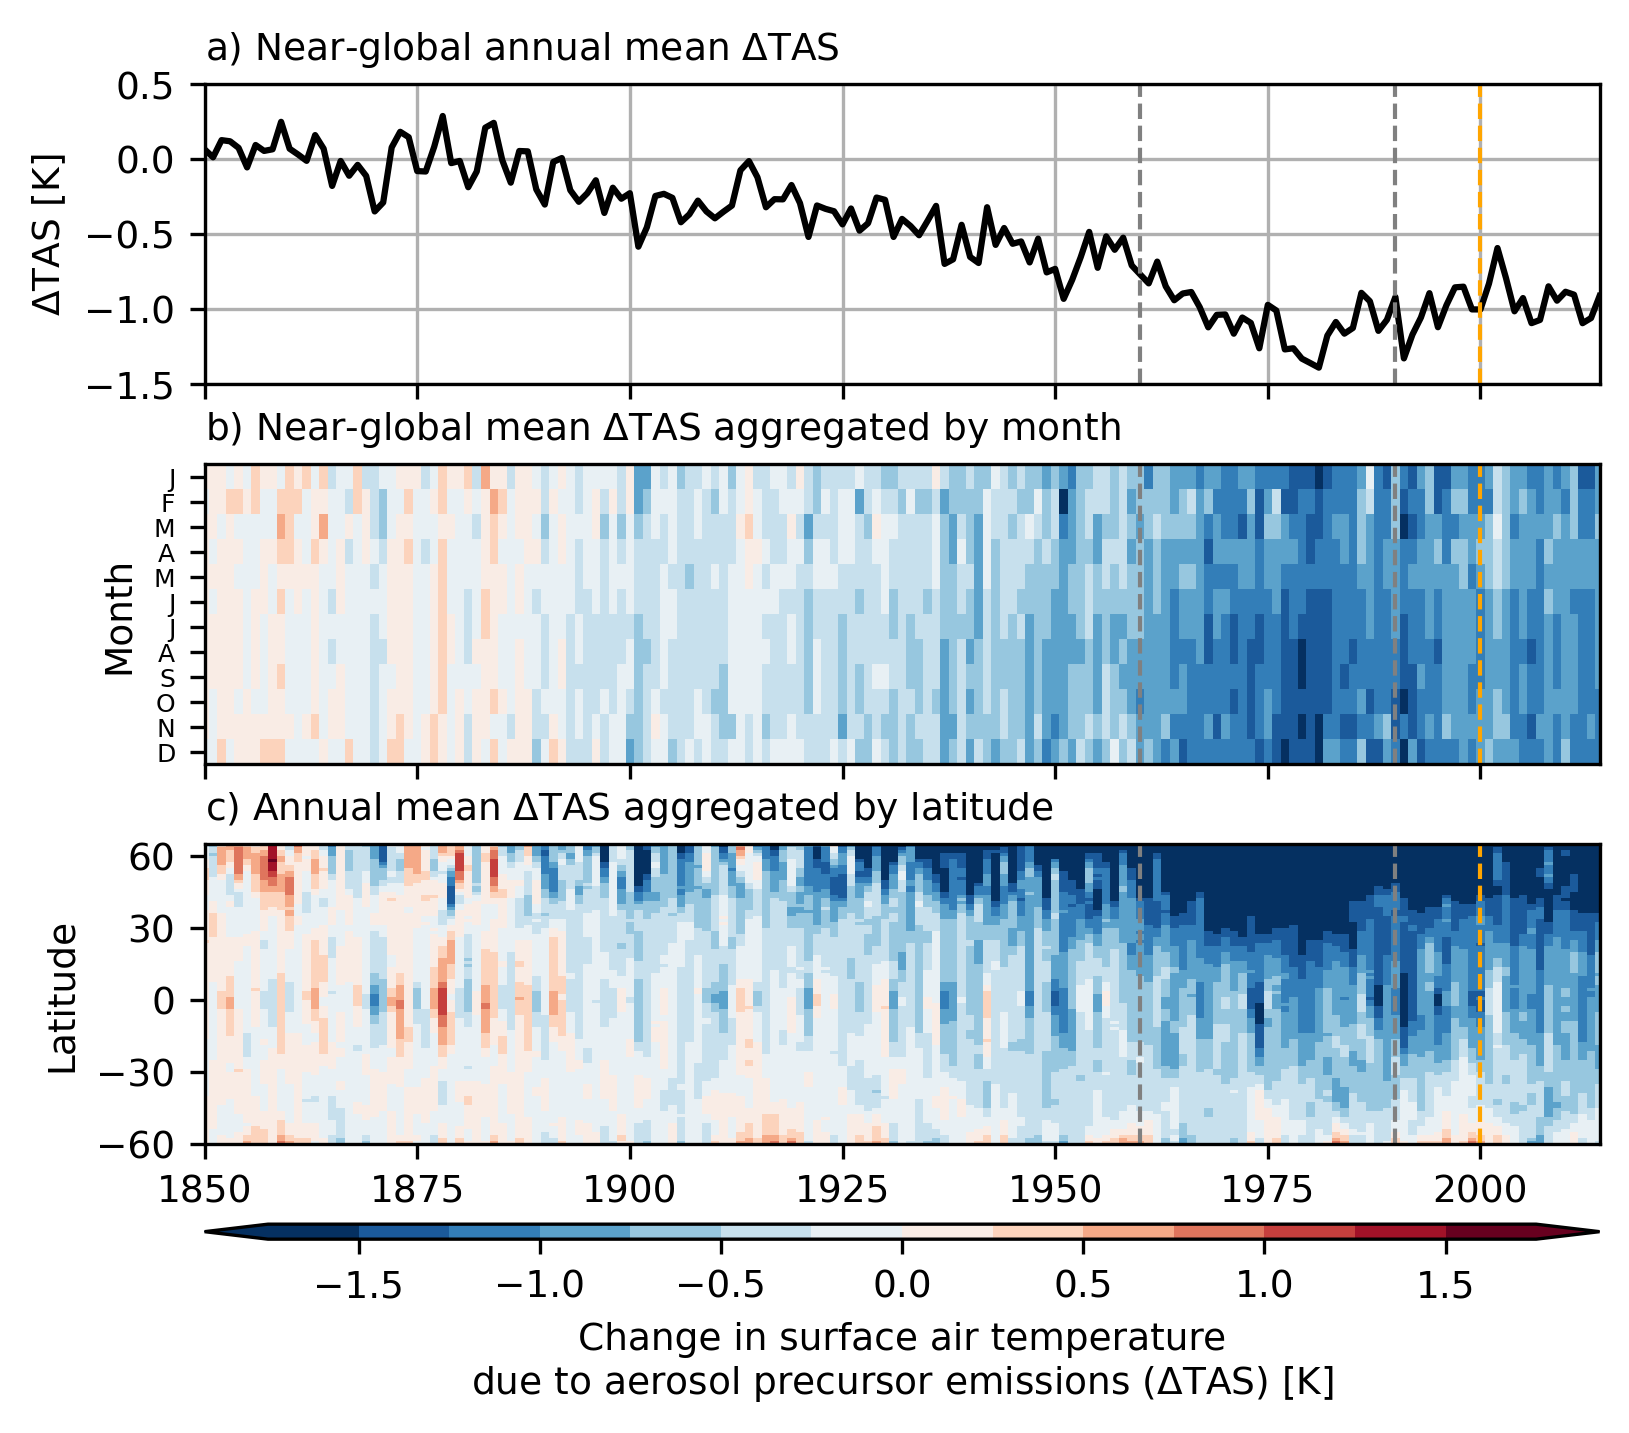
\includegraphics{Chapter4/Figs/tas_change_aerosols.png}
    \caption[Surface air temperature changes due to aerosol precursor emissions]{a) Annual mean surface air temperature changes due to aerosol precursor emissions averaged over latitude 60\textdegree S and 65\textdegree calculated from the difference between \hist{} and \histpiaer{}. b) Near-global mean surface air temperature aggregated by month and year. c) Near-global mean surface air temperature aggregated by month and latitude.}
    \label{fig:ch4:tas-change-aerosol}
\end{figure}

Figure \ref{fig:ch4:tas-change-aerosol} shows the change in near-global mean TAS due to aerosol precursor emissions. Aerosol cooling is strongest in the northern latitudes. At the maximum in the 1980s, aerosols cool down TAS by 1.5 K globally and more than 2 K in the northern hemisphere. After the pothole period, $\Delta$TAS slightly increases, and the Northern Hemisphere is not as cooled by aerosol. 


\begin{figure}
    \centering
    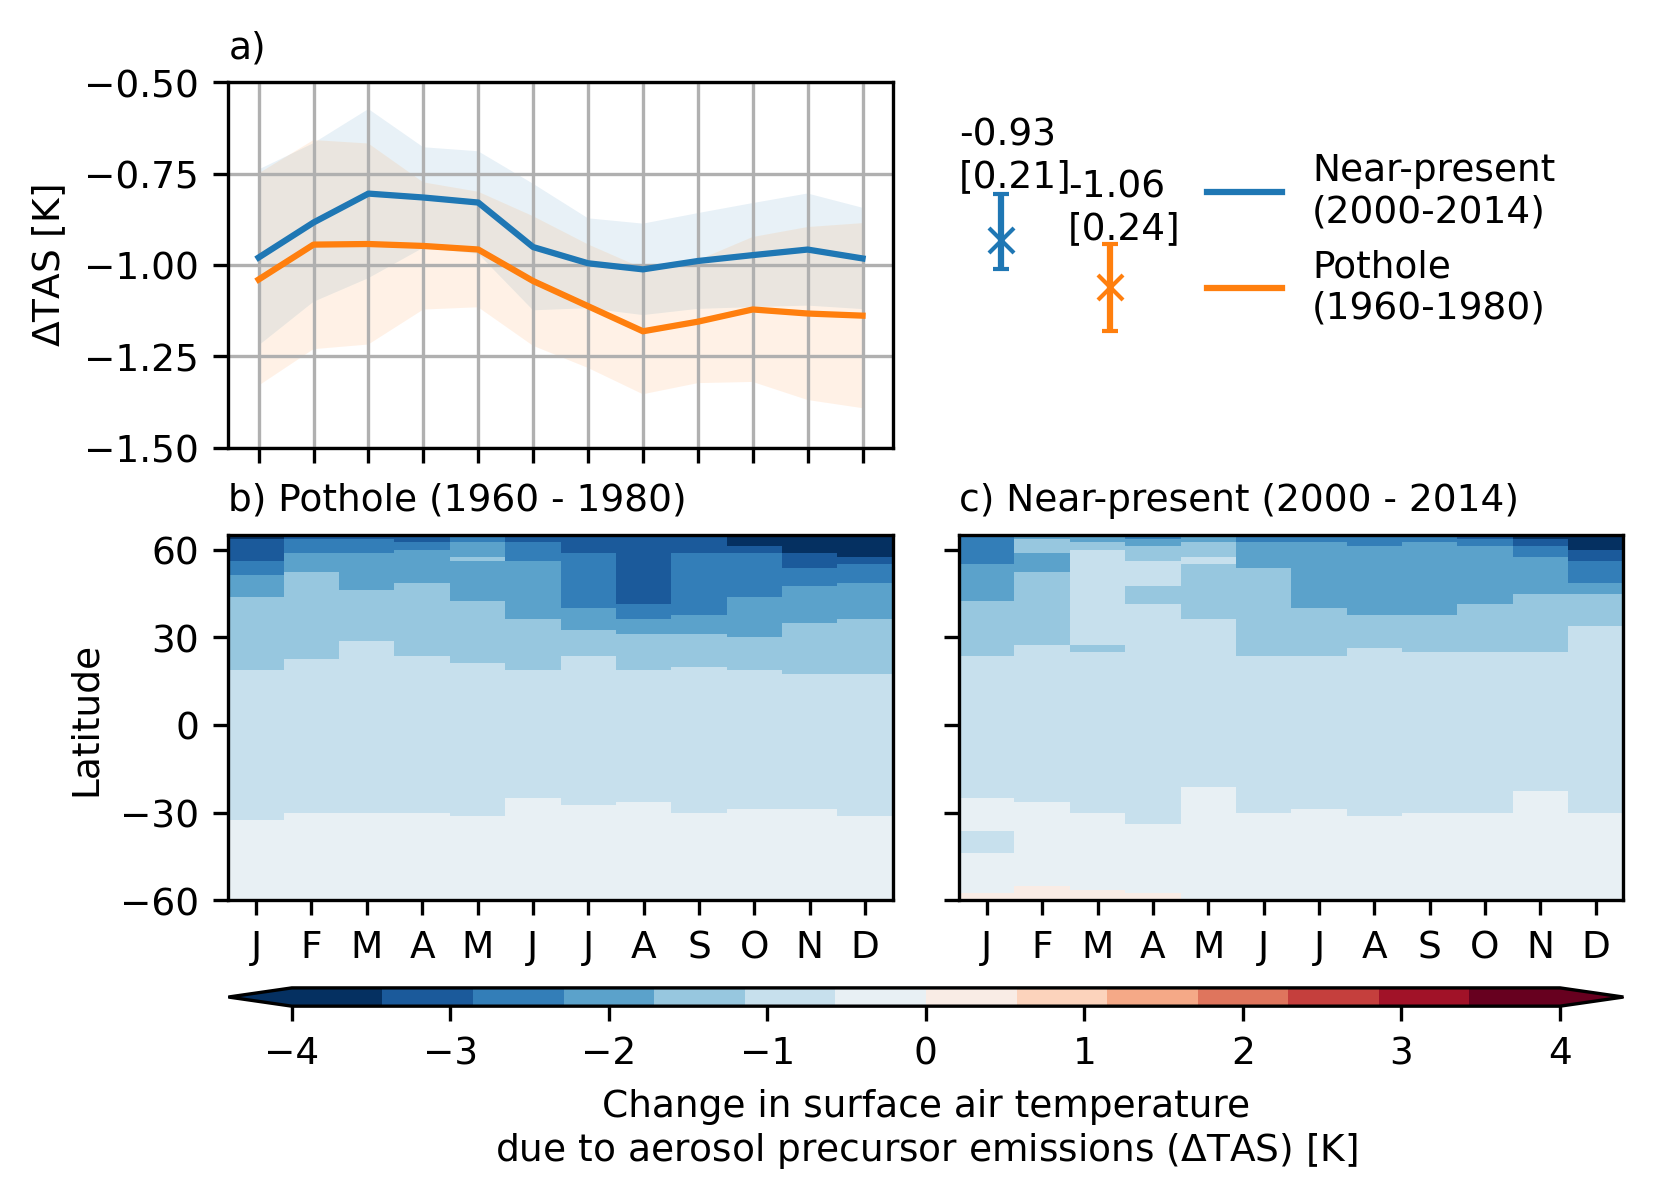
\includegraphics{Chapter4/Figs/tas_range.png}
    \caption[Change in surface air temperature due to aerosol precursor emissions for 1960--1989 and 2000-2014]{a) Near-global mean surface air temperature change due to aerosol precursor emissions (\hist{} minus \histpiaer{}) for the pothole and near-present period averaged over latitude 60\textdegree S and 65\textdegree N aggregated by month. $\Delta$TAS during b) pothole and c) near-present period aggregated by month and latitude. The notation next to a) shows the annual mean $\Delta$TAS and the range (maximum minus minimum) in square brackets.}
    \label{fig:ch4:tas-range}
\end{figure}

Figure \ref{fig:ch4:tas-range} shows the range of cooling between the maximum and minimum between two periods of interest: the pothole period (1960--1989) and near present (2000--2014). Aerosol reduces $\Delta$TAS, with the most significant impact in August in the Northern Hemisphere and the least in March and May. Both periods show a similar trend, but the range of $\Delta$TAS is greater during the pothole period (0.24 compared to 0.21 K)

\section{Conclusions}


% points: oxidants, oxidation, , importance of cloud fraction,  lifetime, cloud, ERF, specific ERF, correlation between SO2_OH and ERF, TAS
This chapter provides systematic view on the impact of \ce{SO2} oxidation in different seasons on aerosol and cloud formation, radiative effects and surface air temperature as simulated by UKESM1. Due to more photochemical production of oxidants in summer. UKESM1 simulates more aerosol particles in summer and shows strong ERF. The change in ERF per unit of \ce{SO2} emissions are reported, showing that \ce{SO2} emitted in summer has 2--4 times more potential to increase ERF. The model captures the seasonal trends in TAS anomaly (a more negative summer anomaly than winter and spring) compared to observation HadCRUT5. The model also shows a strong aerosol cooling during the pothole period compared to the present day, when the model performs well compared to HadCRUT5. While sulfate loading correlates with pothole cooling temperature \citep{zhangRoleAnthropogenicAerosols2021}, we suggest that aerosol loading in summer may contribute more significantly to anomalous cooling. 

Going forward, Other ESMs may benefit from a similar analysis proposed in this Chapter and assist in understanding the role of aerosol formation in this pothole problem. While \ce{SO2} emission in winter has a lower radiation effect and \citet{bellouinRegionalSeasonalRadiative2016} suggests that this could be used in controlled emissions where more \ce{SO2} can be emitted in winter due to lesser climatic impact, this work would like to suggest otherwise. \ce{SO2} emitted in winter has a longer lifetime, it is more likely to cause health impacts and should be considered.


% why do we overestimate cooling during the pothole period and not near present if this is due to seasonal bias? Is there something special about emitting SO2 over Europe/North America compared to China + India?

%\chapter{Regional aerosol formation in the CMIP6 historical period}
% **************************** Define Graphics Path **************************
\ifpdf
    \graphicspath{{Chapter5/Figs/Raster/}{Chapter3/Figs/PDF/}{Chapter5/Figs/}}
\else
    \graphicspath{{Chapter5/Figs/Vector/}{Chapter5/Figs/}}
\fi

% Multiple model results indicate that the global fast precipitation response to regional aerosol forcing scales with global atmospheric absorption \citep{myhrePDRMIPPrecipitationDriver2017}.

% While the emission region does not impact the scale of temperature response, it may impact the aerosol loading and indirectly control the strength of aerosol forcing.

\section*{Abstracts}
This section focuses on regional aspects of aerosol formation. It deals with both annual and seasonal trends. The region of interest includes Northeastern America, Europe, Eastern Asia and South Asia.

NEA and EUR share similar emission trends where SO2 emissions peaked around 1980 and declined. Whereas, emissions from EAS and SAS are on the increase in the near present. 

\section{Introduction}
A modelling study shows that the production of oxidants over different regions may be different \cite{zhangTroposphericOzoneChange2016}. Another model study evaluates how black carbon aerosol emission at different locations affects ERF differently \citep{williamsStrongControlEffective2022}

Furthermore, geographic location can substantially influence the cooling potential of a given aerosol emission \citep{persadDivergentGlobalscaleTemperature2018}. Relative climate effects of combined sulfate, black carbon, and organic carbon aerosol emissions equivalent to China's total annual emission in 2000 result in different cooling potential.

In addition to temperature impact, which seems to be homogeneous irrespective of the emission region. Multiple model results indicate that the global fast precipitation response to regional aerosol forcing scales with global atmospheric absorption \citep{myhrePDRMIPPrecipitationDriver2017}

This means that the emission region does not impact the scale of temperature response. howeve, the region of emission may impact the aerosol loading.

However, this study investigates from aerosol not emission and here we are interested in the oxidation potential in different region. we focus on regions where the change in emission has been the largest: North America, Europe, India, and China



% From AAmas https://acp.copernicus.org/articles/16/7451/2016/
Emissions metrics have normally been calculated for
global emissions. However, for SLCFs, due to their short
lifetimes compared to large-scale atmospheric mixing times,
and because the chemistry and radiative effects on climate
depends on the regional physical conditions, even the global
mean radiative forcing depends on the region of emissions
(Fuglestvedt et al., 1999; Wild et al., 2001; e.g., Berntsen et
al., 2005; Naik et al., 2005). Then, the emission metric val-
ues will vary for different emission locations (Fuglestvedt
et al., 2010). In addition, distinct patterns in the tempera-
ture response appear from all forcings (Boer and Yu, 2003;
Shindell et al., 2010). A growing literature investigates how
the weights of the emission metrics change as emissions
from different regions of the world are considered. Collins
et al. (2013) assessed variations in emission metrics for four
different regions (East Asia, Europe, North America, and
South Asia) for aerosols and ozone precursors, based on
radiative forcings from consistent multimodel experiments
from the Hemispheric Transport of Air Pollution (HTAP) ex-
periments given by Yu et al. (2013) and Fry et al. (2012).
Collins et al. (2010) also investigated how emission met-
ric values differ between regions, including vegetation re-
sponses. Bond et al. (2011) quantified differences in RFs for
BC and OC emissions from different locations and types of
emissions

\subsection{\texorpdfstring{\ce{SO2}}{SO2} emissions trends over different regions}

Zonal asymmetry of anthropogenic aerosol forcing in the recent decades \citep{diaoAnthropogenicAerosolEffects2021}


Explain the emissions trends over NEA, EUR, EAS, SAS. 

The distribution of aerosol by each source is explored in \citet{yangGlobalSourceAttribution2017}. Sulfate aeroosl can be transported further from source area.


\subsection{Annual cycle of oxidant trends and their drivers for different regions}



%\chapter{Summary, Conclusions and Future Directions}
% **************************** Define Graphics Path **************************
\ifpdf
    \graphicspath{{Chapter6/Figs/Raster/}{Chapter6/Figs/PDF/}{Chapter6/Figs/}}
\else
    \graphicspath{{Chapte6/Figs/Vector/}{Chapter6/Figs/}}
\fi


\section{Summary of key results}

\section{Future directions}

\subsection{piSO2 simulations}

\subsection{Expanding the analysis to other ESMs}

\subsection{Implication to TAS and the pothole problem}
% The preliminary work I have done analysing the TAS anomaly 

\subsection{Looking beyond SO2 oxidation}
% how about black carbon and organic soa? Does this affect ERF only seasonally?




%\include{Chapter7/chapter7}



% ********************************** Back Matter *******************************
% Backmatter should be commented out, if you are using appendices after References
%\backmatter

% ********************************** Bibliography ******************************
\begin{spacing}{0.9}

% To use the conventional natbib style referencing
% Bibliography style previews: http://nodonn.tipido.net/bibstyle.php
% Reference styles: http://sites.stat.psu.edu/~surajit/present/bib.htm

\bibliographystyle{apalike}
%\bibliographystyle{unsrt} % Use for unsorted references  
%\bibliographystyle{plainnat} % use this to have URLs listed in References
\cleardoublepage
\bibliography{References/references} % Path to your References.bib file


% If you would like to use BibLaTeX for your references, pass `custombib' as
% an option in the document class. The location of 'reference.bib' should be
% specified in the preamble.tex file in the custombib section.
% Comment out the lines related to natbib above and uncomment the following line.

%\printbibliography[heading=bibintoc, title={References}]


\end{spacing}

% ********************************** Appendices ********************************

\begin{appendices} % Using appendices environment for more functunality

%!TEX root = ../thesis.tex
% ******************************* Thesis Appendix A ****************************
\chapter{Supplementary information for Chapter \ref{ch4:title}} 

\section{ESMs included in the analysis of pothole cooling}

\begin{small}
\begin{longtable}{>{\raggedright}p{3.25cm} >{\raggedright}p{3.25cm} >{\raggedright}p{3.5cm} >{\raggedright\arraybackslash}p{3.5cm}}
    \caption[Information of models included in the study by \citet{zhangRoleAnthropogenicAerosols2021}]{Information of models included in the study by \citet{zhangRoleAnthropogenicAerosols2021}}
    \label{tab:zhang-model}
    \\
    \toprule
     Model developer (Model) & Tropospheric chemistry model & Sulfur chemistry scheme & Aerosol scheme \\
     \midrule
     \endfirsthead

    \toprule
     Model developer (Model) & Tropospheric chemistry model & Sulfur chemistry scheme & Aerosol scheme \\
     \midrule
     \endhead
     
     \bottomrule
     \endlastfoot

     
     Met Office’s Hadley Centre for Climate Prediction and Research; MOHC (UKESM1-0-LL) Ref. \citet{sellarUKESM1DescriptionEvaluation2019,archibaldDescriptionEvaluationUKCA2020,mulcahyDescriptionEvaluationAerosol2020}  & UKCA (United Kingdom Chemistry and Aerosol) model with unified stratospheric-tropospheric chemistry (StratTrop) & Prognostic oxidant fields. Prognostic sulfur chemistry. & Aerosol scheme GLOMAP-mode. Two-moment, five size modes. 4 species: sulfate (\ce{SO4}), black carbon (BC), organic matter (OM) and sea salt. \\
     \midrule
     Norwegian Climate Center; NCC (NorESM2-LM). Ref. \citet{kirkevagProductiontaggedAerosolModule2018, selandOverviewNorwegianEarth2020} & Atmosphere model component CAM6-Nor built improvements on the CAM6 version from CESM2.1 & Diagnostic tropospheric oxidant fields: OH, \ce{O3}, \ce{H2O2}.  Prognostic  sulfur chemistry & 4 aerosol modes. 6 species: SOA, BC, \ce{SO4}, OM, Seasalt, and dust.  \\ 
     \midrule
     Max Planck Institute for Meteorology; MPI (MPI-ESM-1-2-HAM) Ref. \citet{neubauerGlobalAerosolClimate2019,neubauerHAMMOZConsortiumMPIESM12HAM2019,tegenGlobalAerosolClimate2019} & Atmospheric Model Component ECHAM6.3. &  Diagnostic oxidant fields: OH, \ce{H2O2}, \ce{NO2}, \ce{O3}, and \ce{NO3}. Prognostic sulfur chemistry. & Aerosol scheme HAM2.3. Two-moment. 7 modes: 4 soluble and 3 insoluble \\
     \midrule
     US Department of Commerce/ NOAA/Geophysical Fluid Dynamics Laboratory; GFDL (GFDL-ESM4) Ref. \citet{zhaoGFDLGlobalAtmosphere2018, heldStructurePerformanceGFDL2019, dunneGFDLEarthSystem2020} & Atmospheric component AM4.1 & Prognostic oxidant fields: OH, \ce{O3}, \ce{H2O2}, \ce{NO3}. Prognostic sulfur chemistry. & 5 aerosol types: sulfate, dust, black carbon, organic carbon, and sea salt.  \\
     \midrule
     European consortium of meteorological services, research institutes, and high-performance computing centres (EC-Earth-AerChem) Ref. \citet{vannoijeECEarth3AerChemGlobalClimate2021} & Aerosols and atmospheric chemistry are simulated with the Tracer Model version 5 (TM5), specifically release 3.0 of the massively parallel version of TM5 (TM5-mp 3.0). & The model includes aqueous-phase reactions for total dissolved sulfur dioxide oxidation & Modal aerosol microphysical scheme M7. 5 aerosol types: \ce{SO4}, BC, OA, sea salt, and mineral dust. 7 modes: 4 water-soluble and 3 insoluble modes  \\
     \midrule
     Beijing Climate Center; BCC (BCC-ESM1) Ref. \citet{zhangBCCESM1ModelDatasets2021} &  Atmospheric component is BCCAGCM3-Chem based on MOZART2 & Prognostic oxidant fields. Prognostic sulfur chemistry. & 5 aerosol species: \ce{SO4}, OC, BC, soil dust, and sea salt \\


\end{longtable}
\end{small}


\section{Supplementary figures}
\begin{figure}
    \centering
    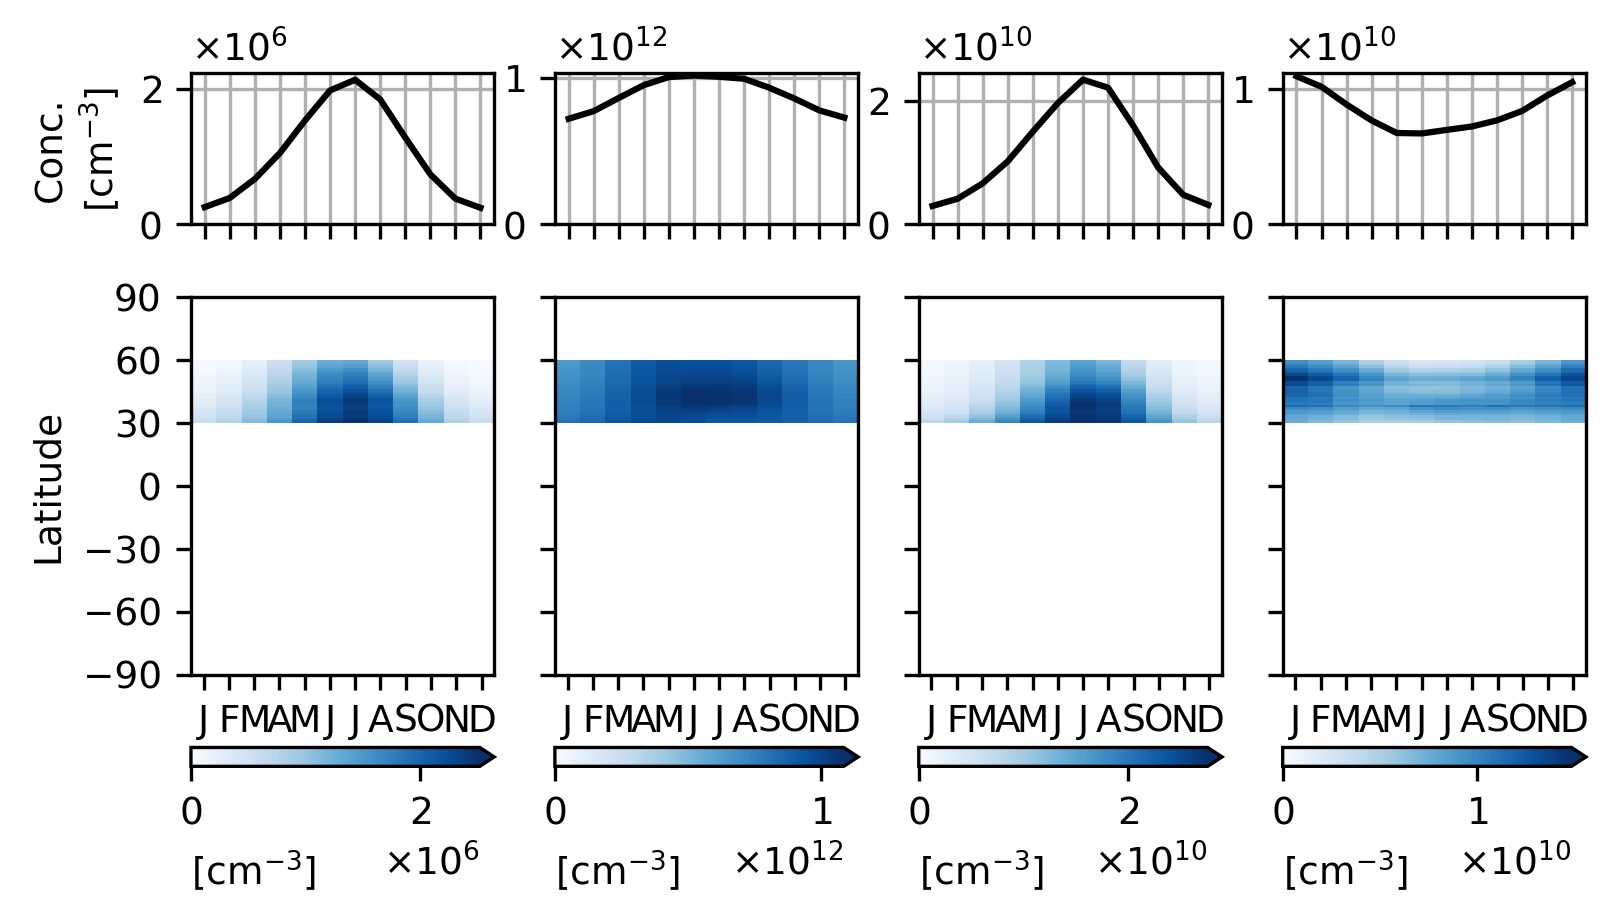
\includegraphics{Appendix1/figs/seasonal_oxidant_1980_lat30-60.png}
    \caption{Mean oxidant concentration between 1980 and 1989 from the surface up to 5 km and latitude 30 to 60\textdegree N }
    \label{fig:app1:seasonal-oxidant-30-60}
\end{figure}

\begin{figure}
    \centering
    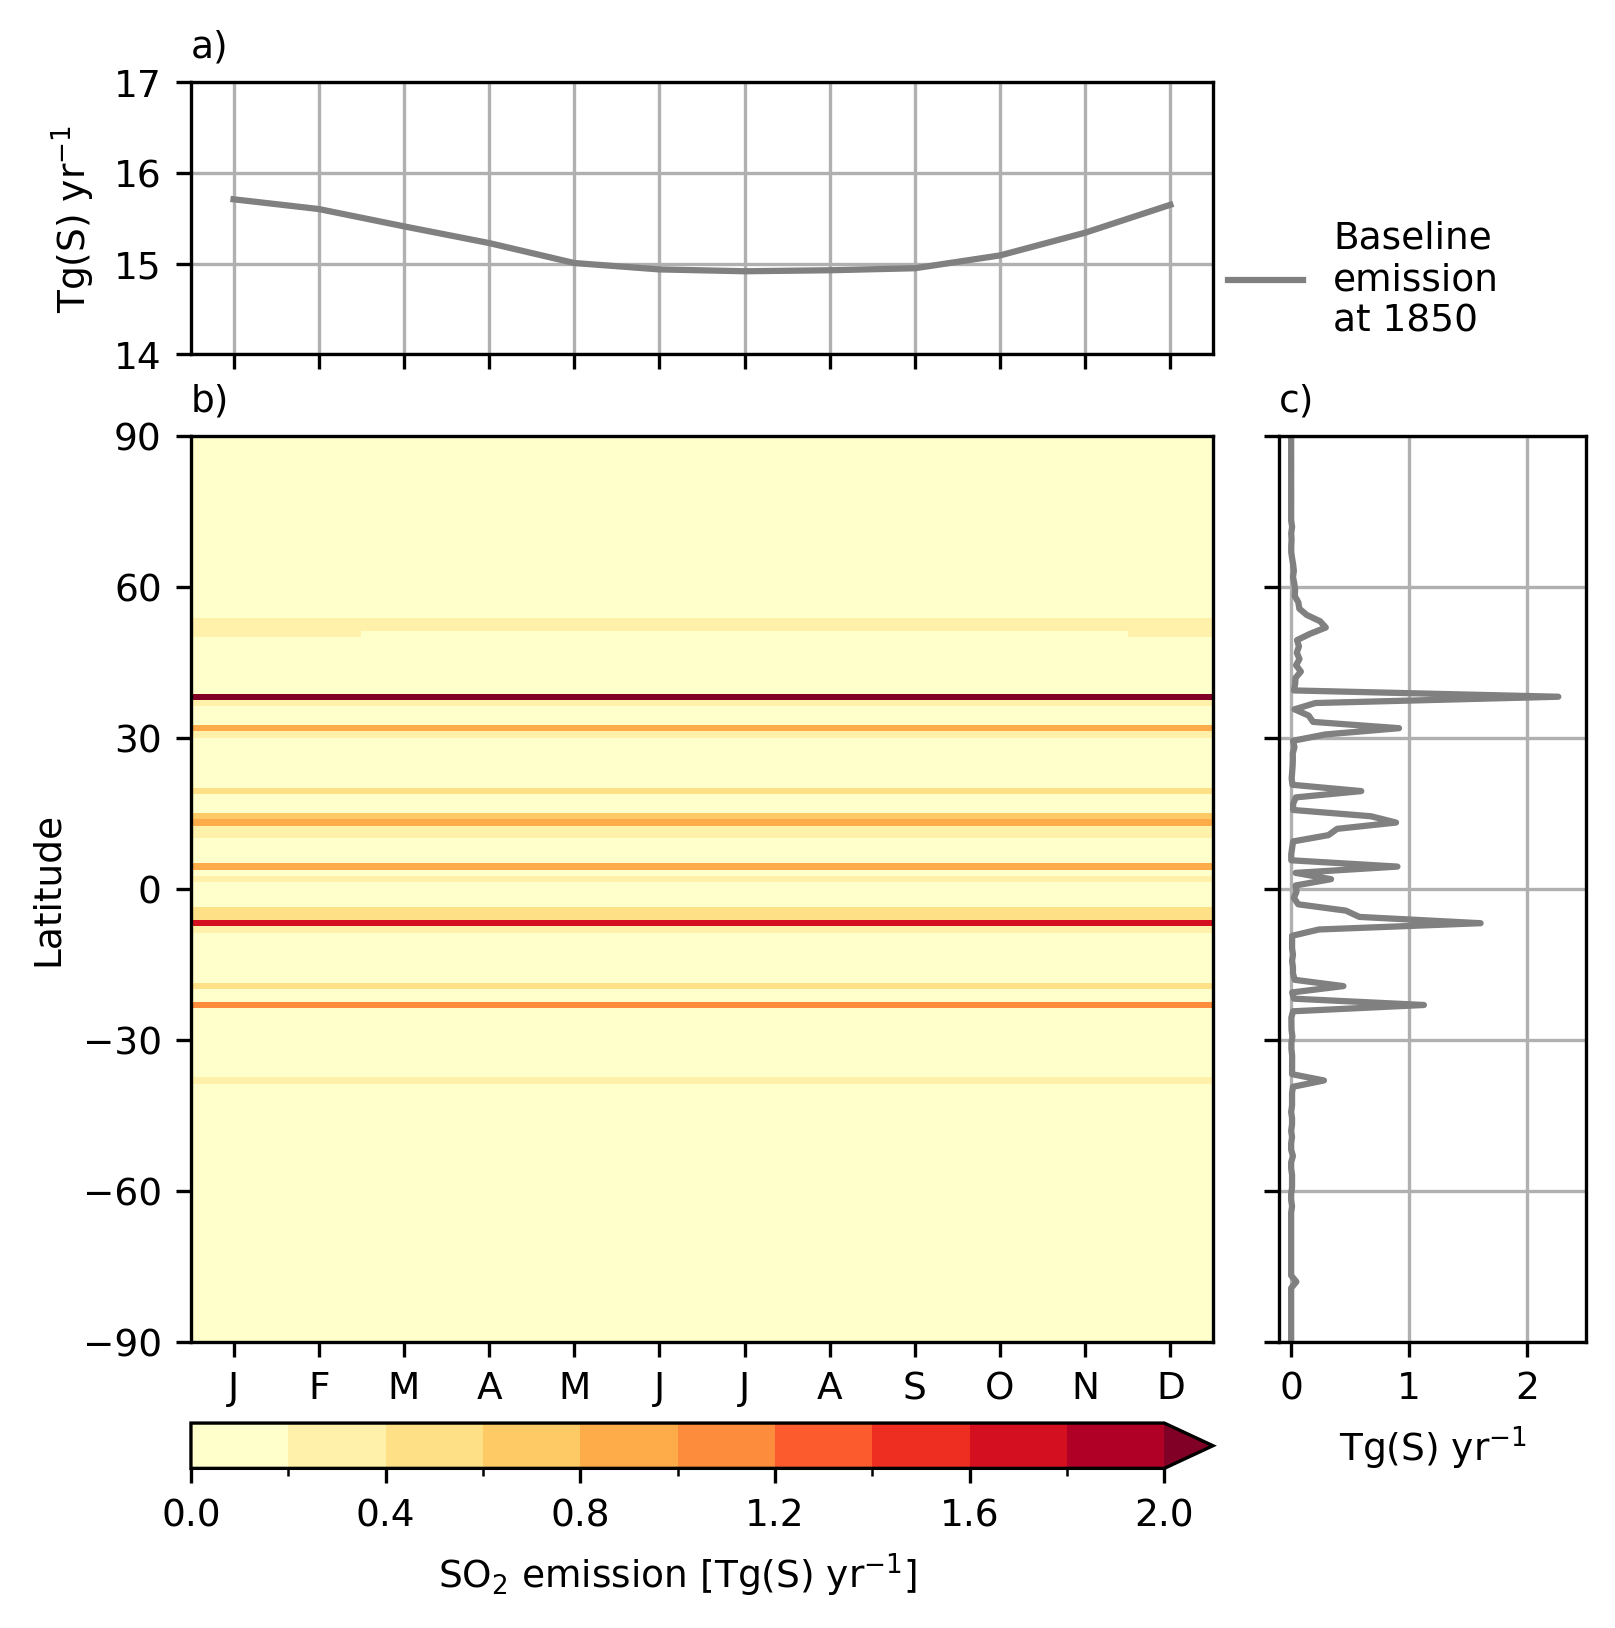
\includegraphics{Appendix1/figs/emiso2_monthly_1850.png}
    \caption[\ce{SO2} emissions between 1850--1860]{\ce{SO2} emissions between 1850--1860}
    \label{fig:app1:seasonal-emiso2-1850}
\end{figure}

\begin{figure}
    \centering
    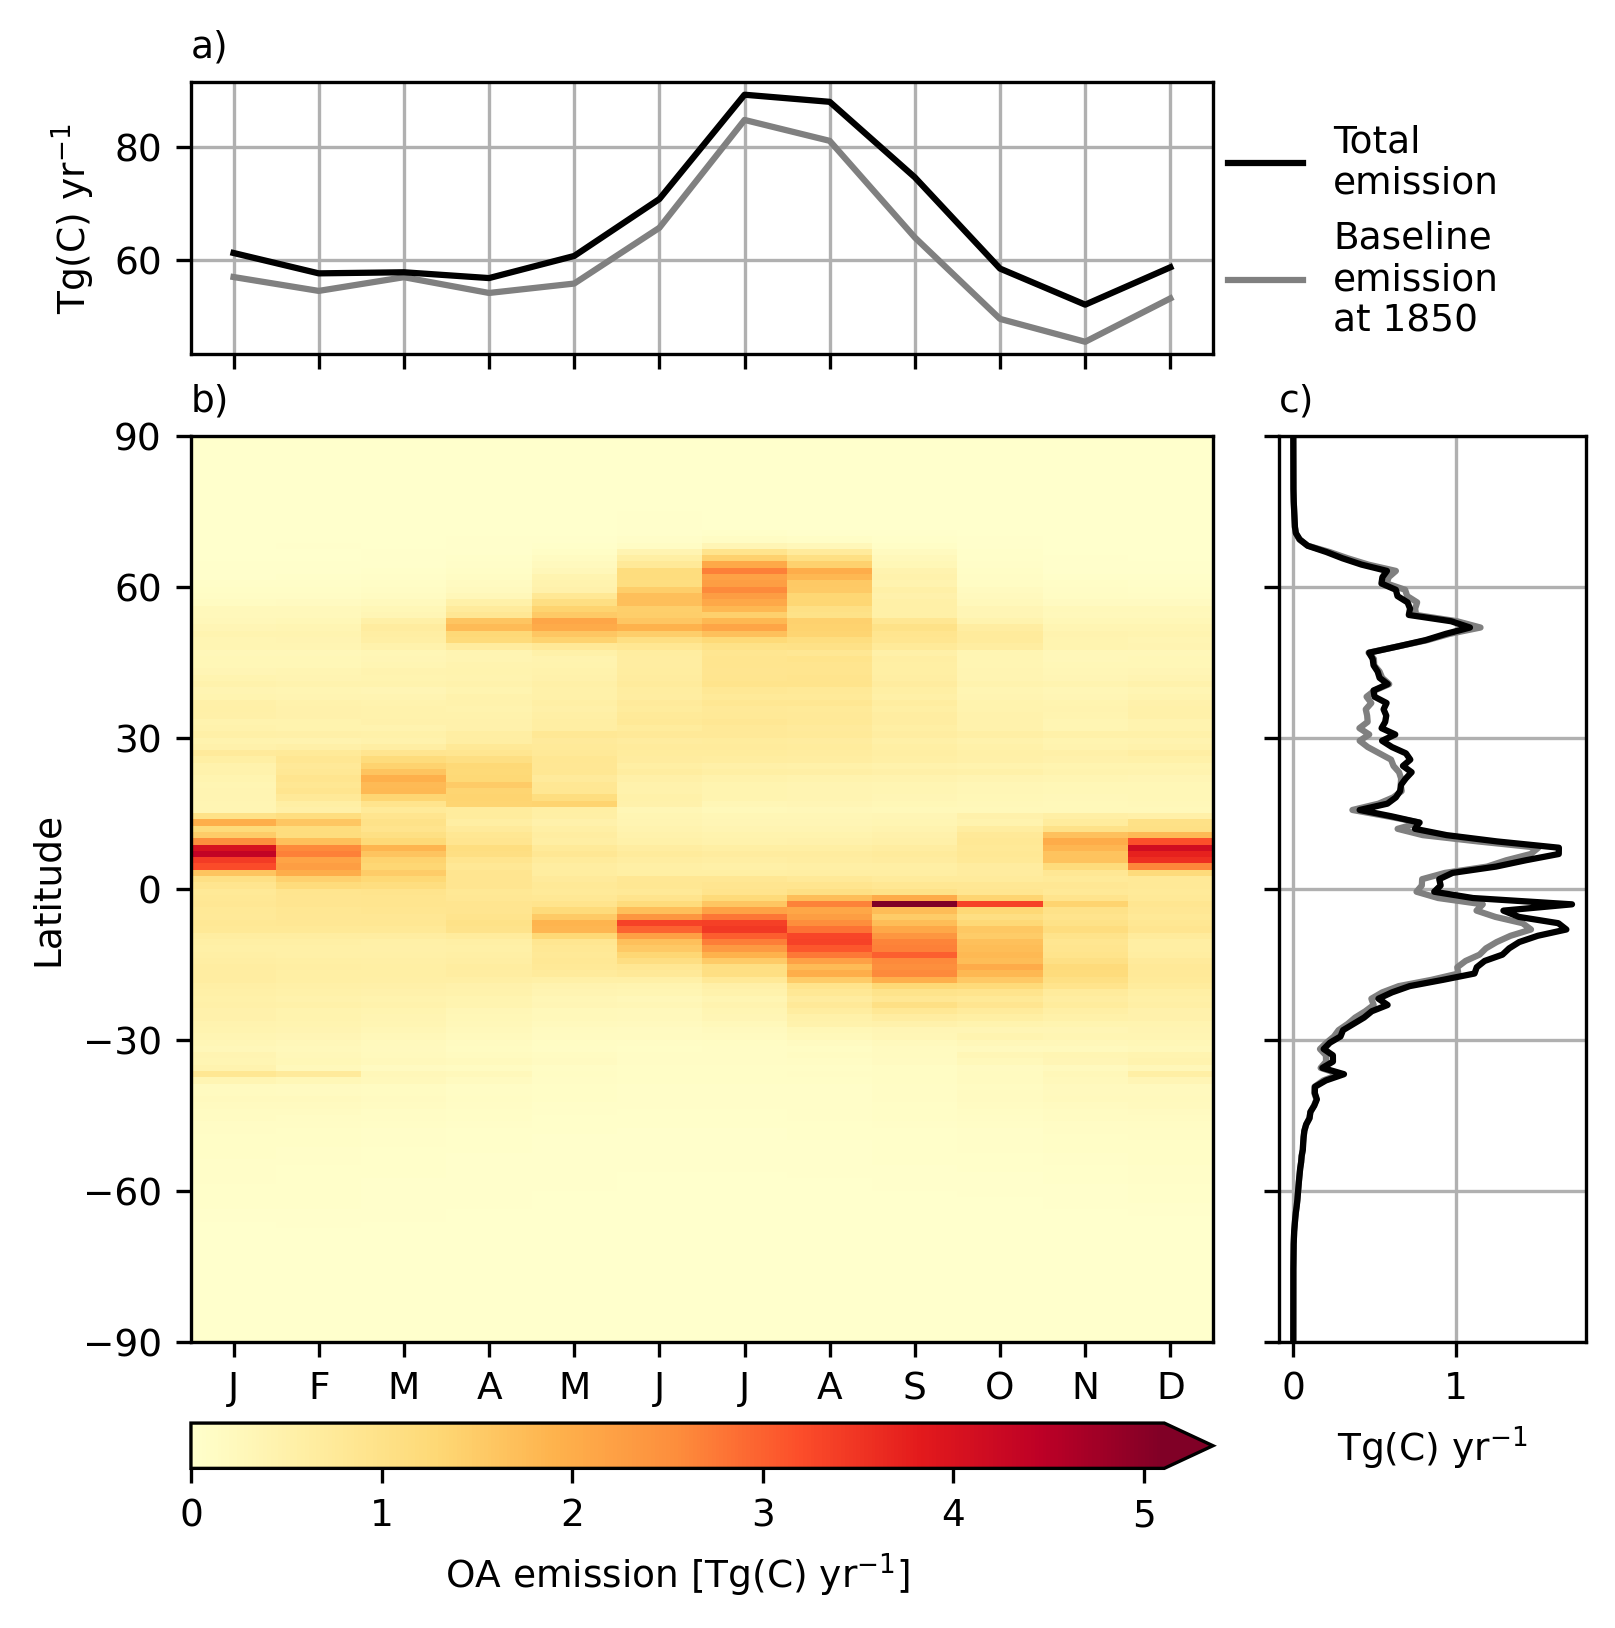
\includegraphics{Appendix1/figs/emioa_monthly_pothole.png}
    \caption[Organic aerosol emissions between 1960--1989]{Organic aerosol emissions between 1960--1989. This is the total emission of primary organic aerosol (POA) and total production of secondary organic aerosol (SOA).}
    \label{fig:app1:seasonal-emioa-pothole}
\end{figure}

\begin{figure}
    \centering
    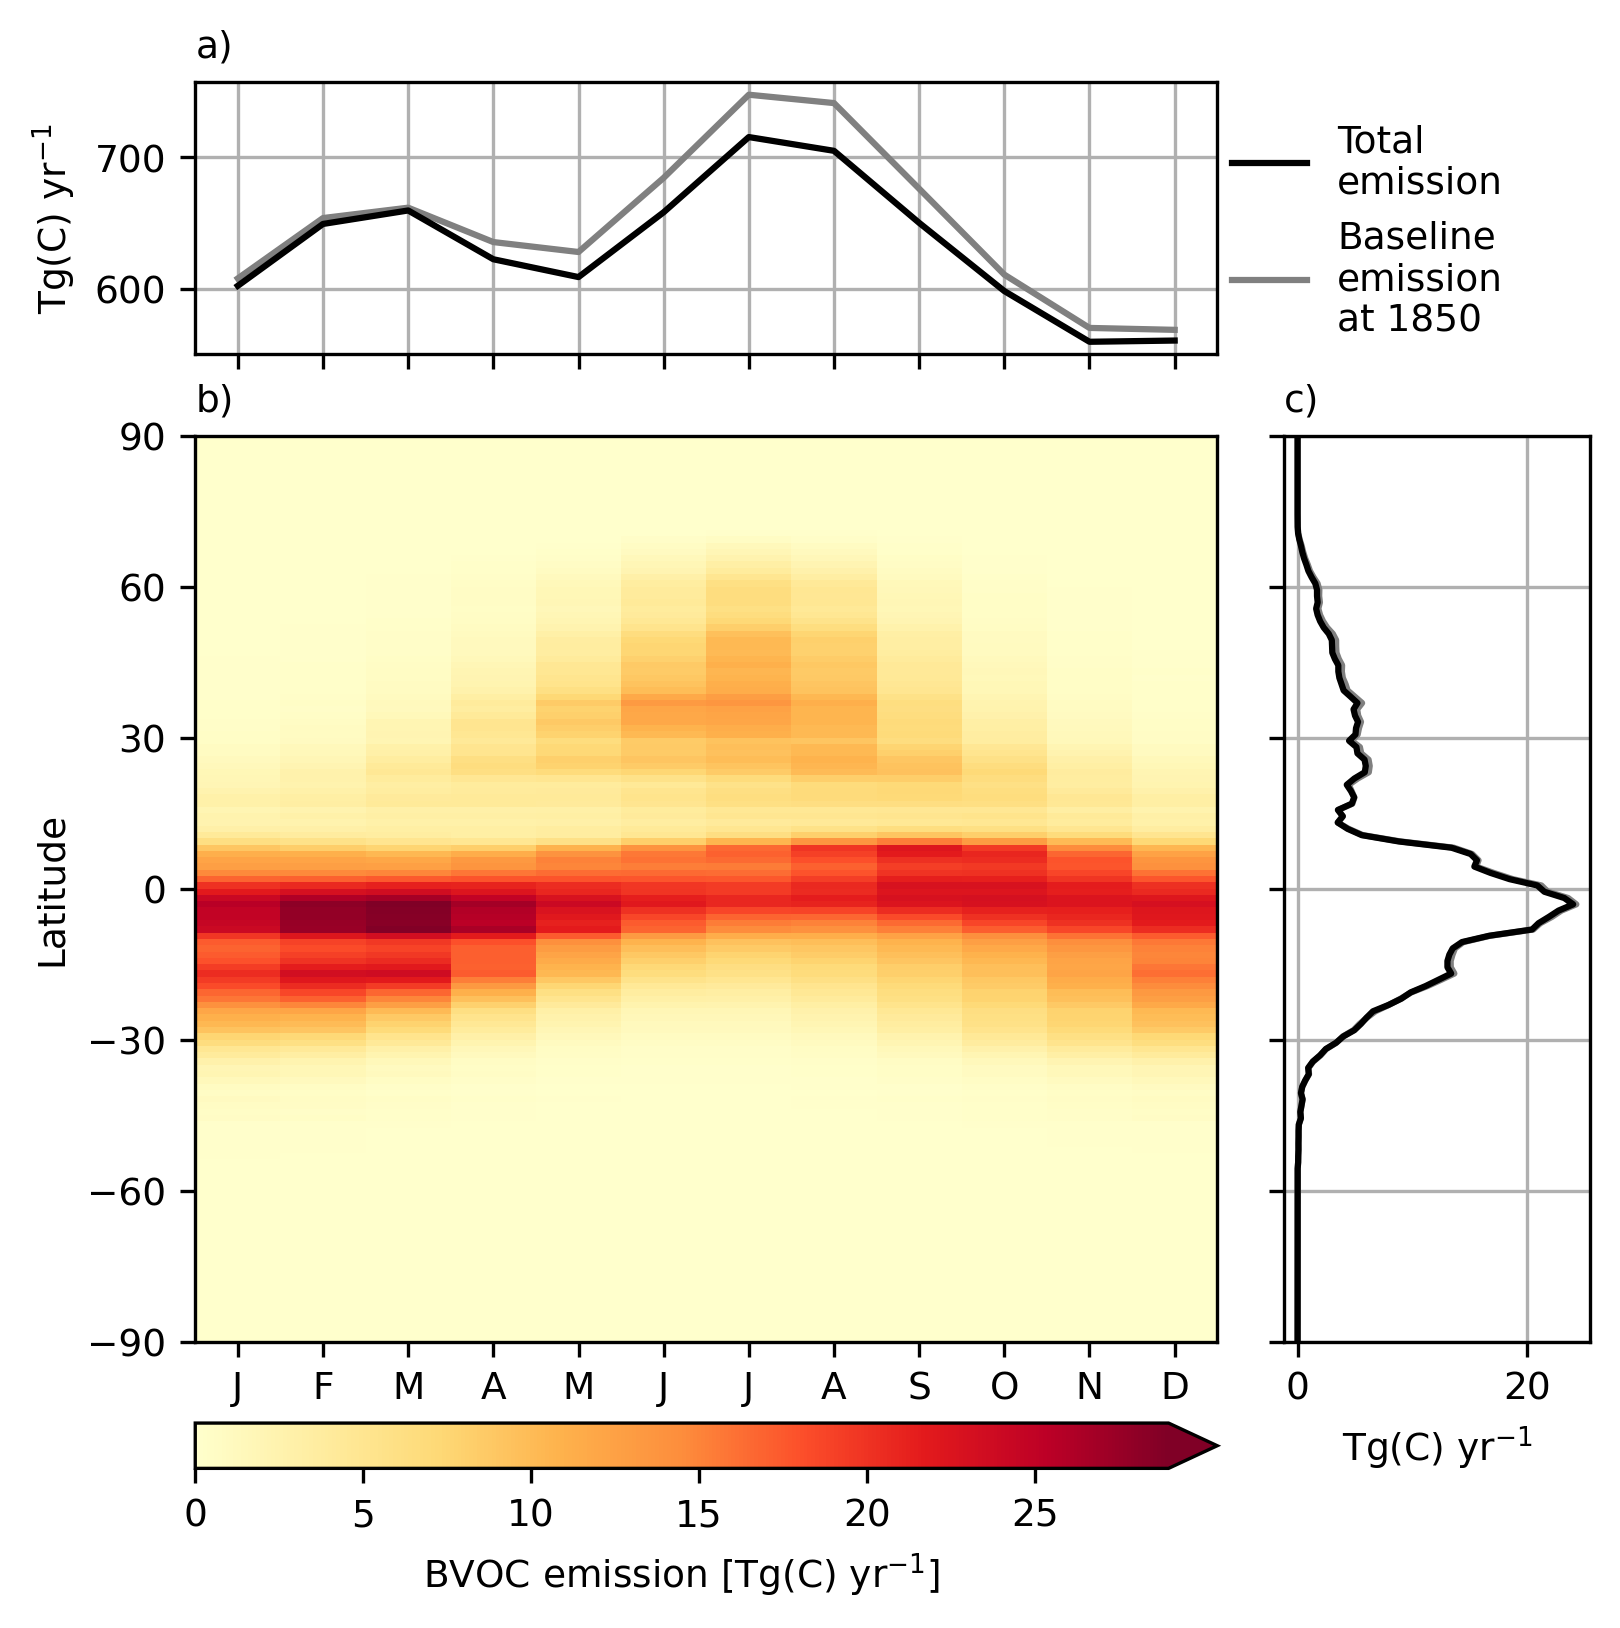
\includegraphics{Appendix1/figs/emibvoc_monthly_pothole.png}
    \caption[Biogenic volatile organic compound emissions between 1960--1989]{Biogenic volatile organic compound emissions between 1960--1989. Isoprene and Monoterpene only. Acetone and Methanol, although produced by JULES, are not used by UKCA, which reads from ancillary.}
    \label{fig:app1:seasonal-emibvoc-pothole}
\end{figure}

\begin{figure}
    \centering
    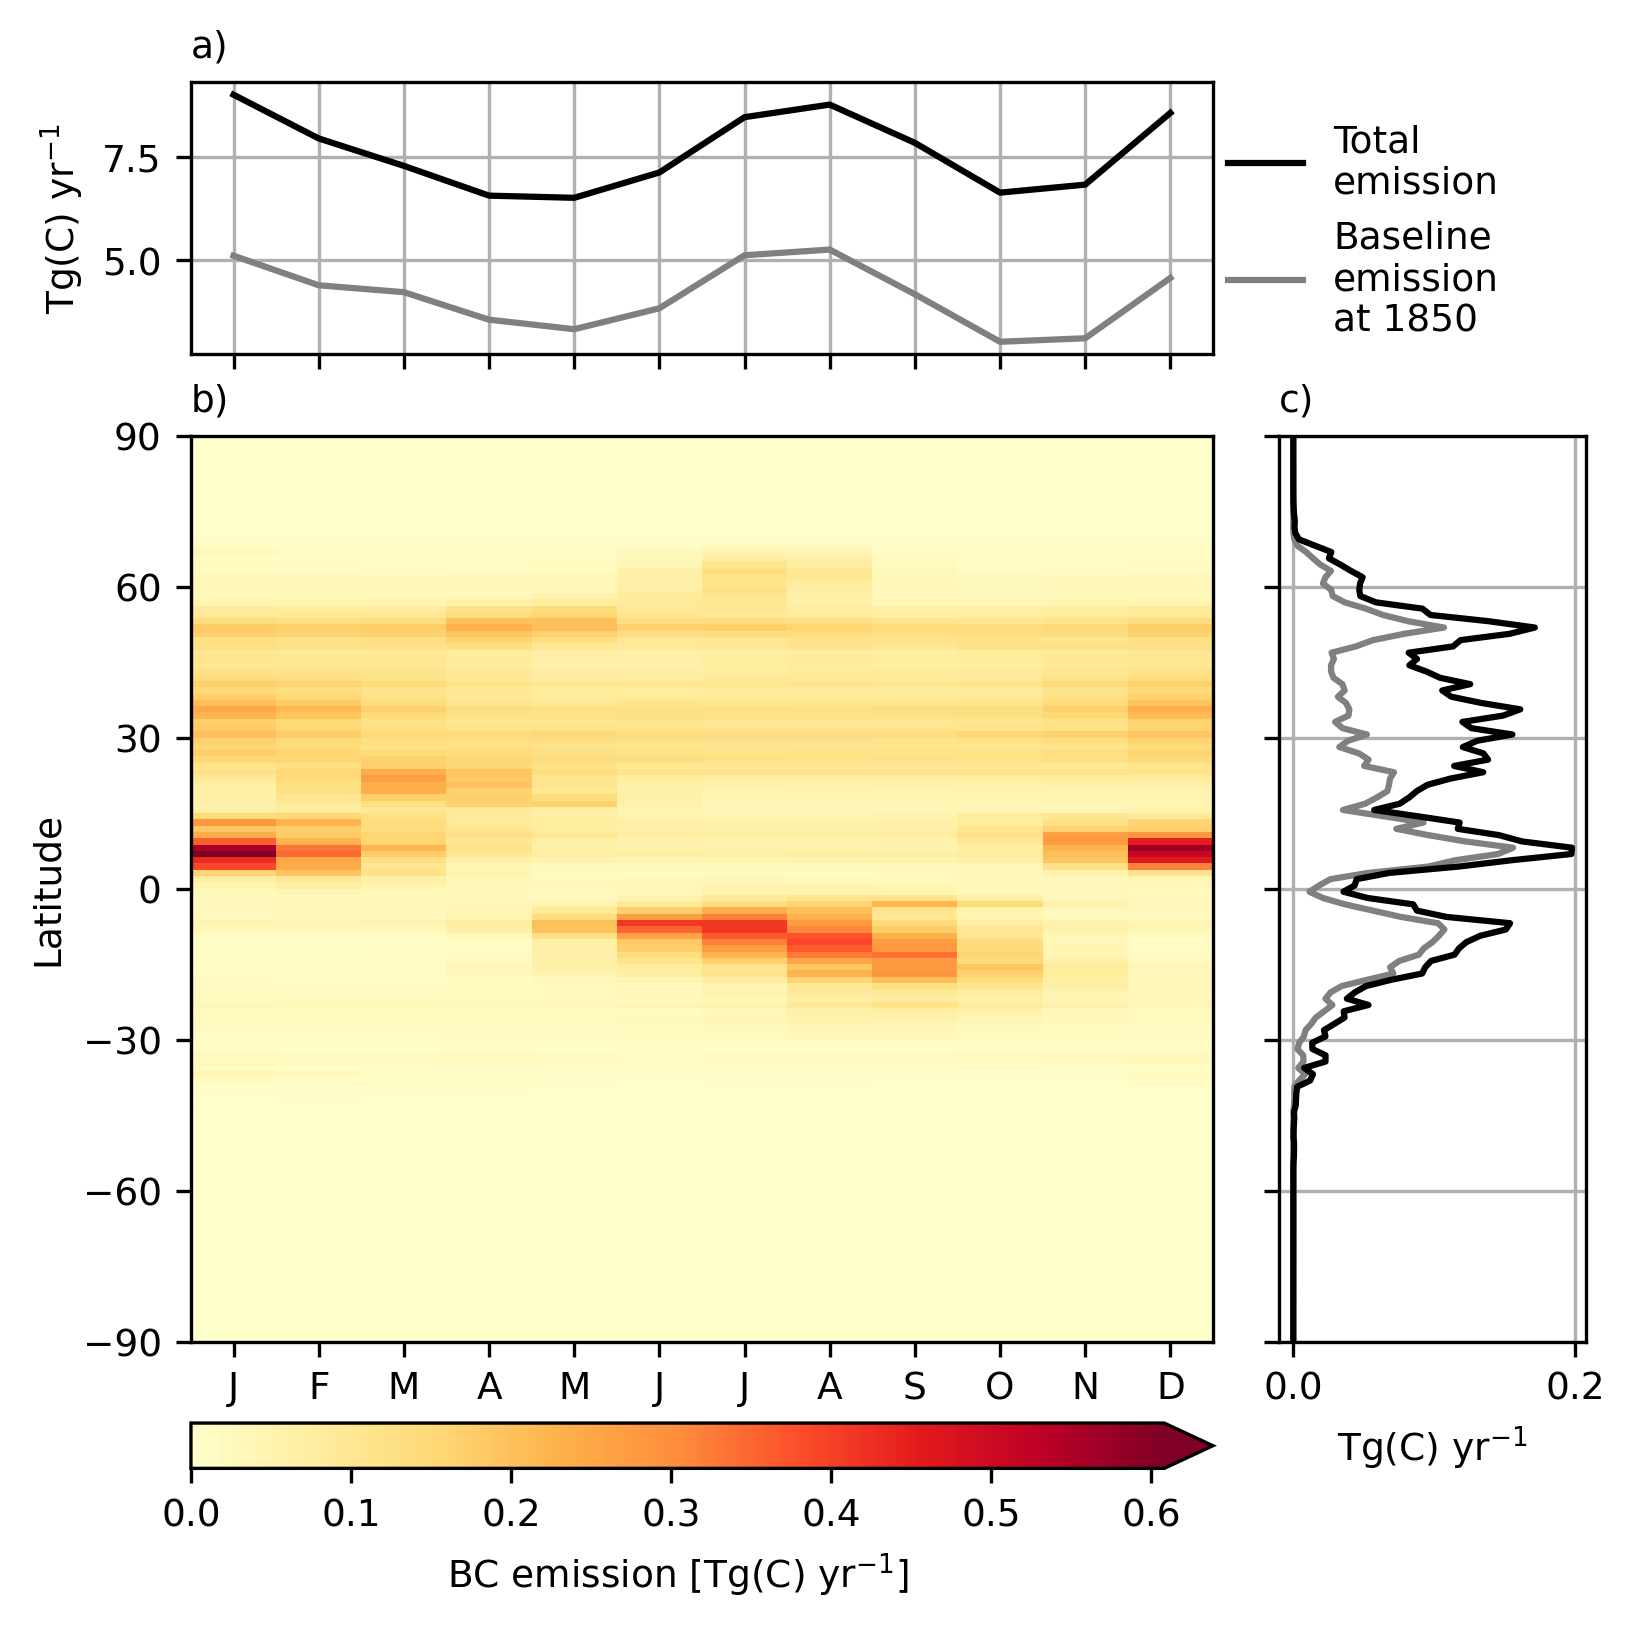
\includegraphics{Appendix1/figs/emibc_monthly_pothole.png}
    \caption{Black carbon (BC) emissions at 1850 between 1960--1989.}
    \label{fig:app1:seasonal-emibc-pothole}
\end{figure}

\begin{figure}
    \centering
    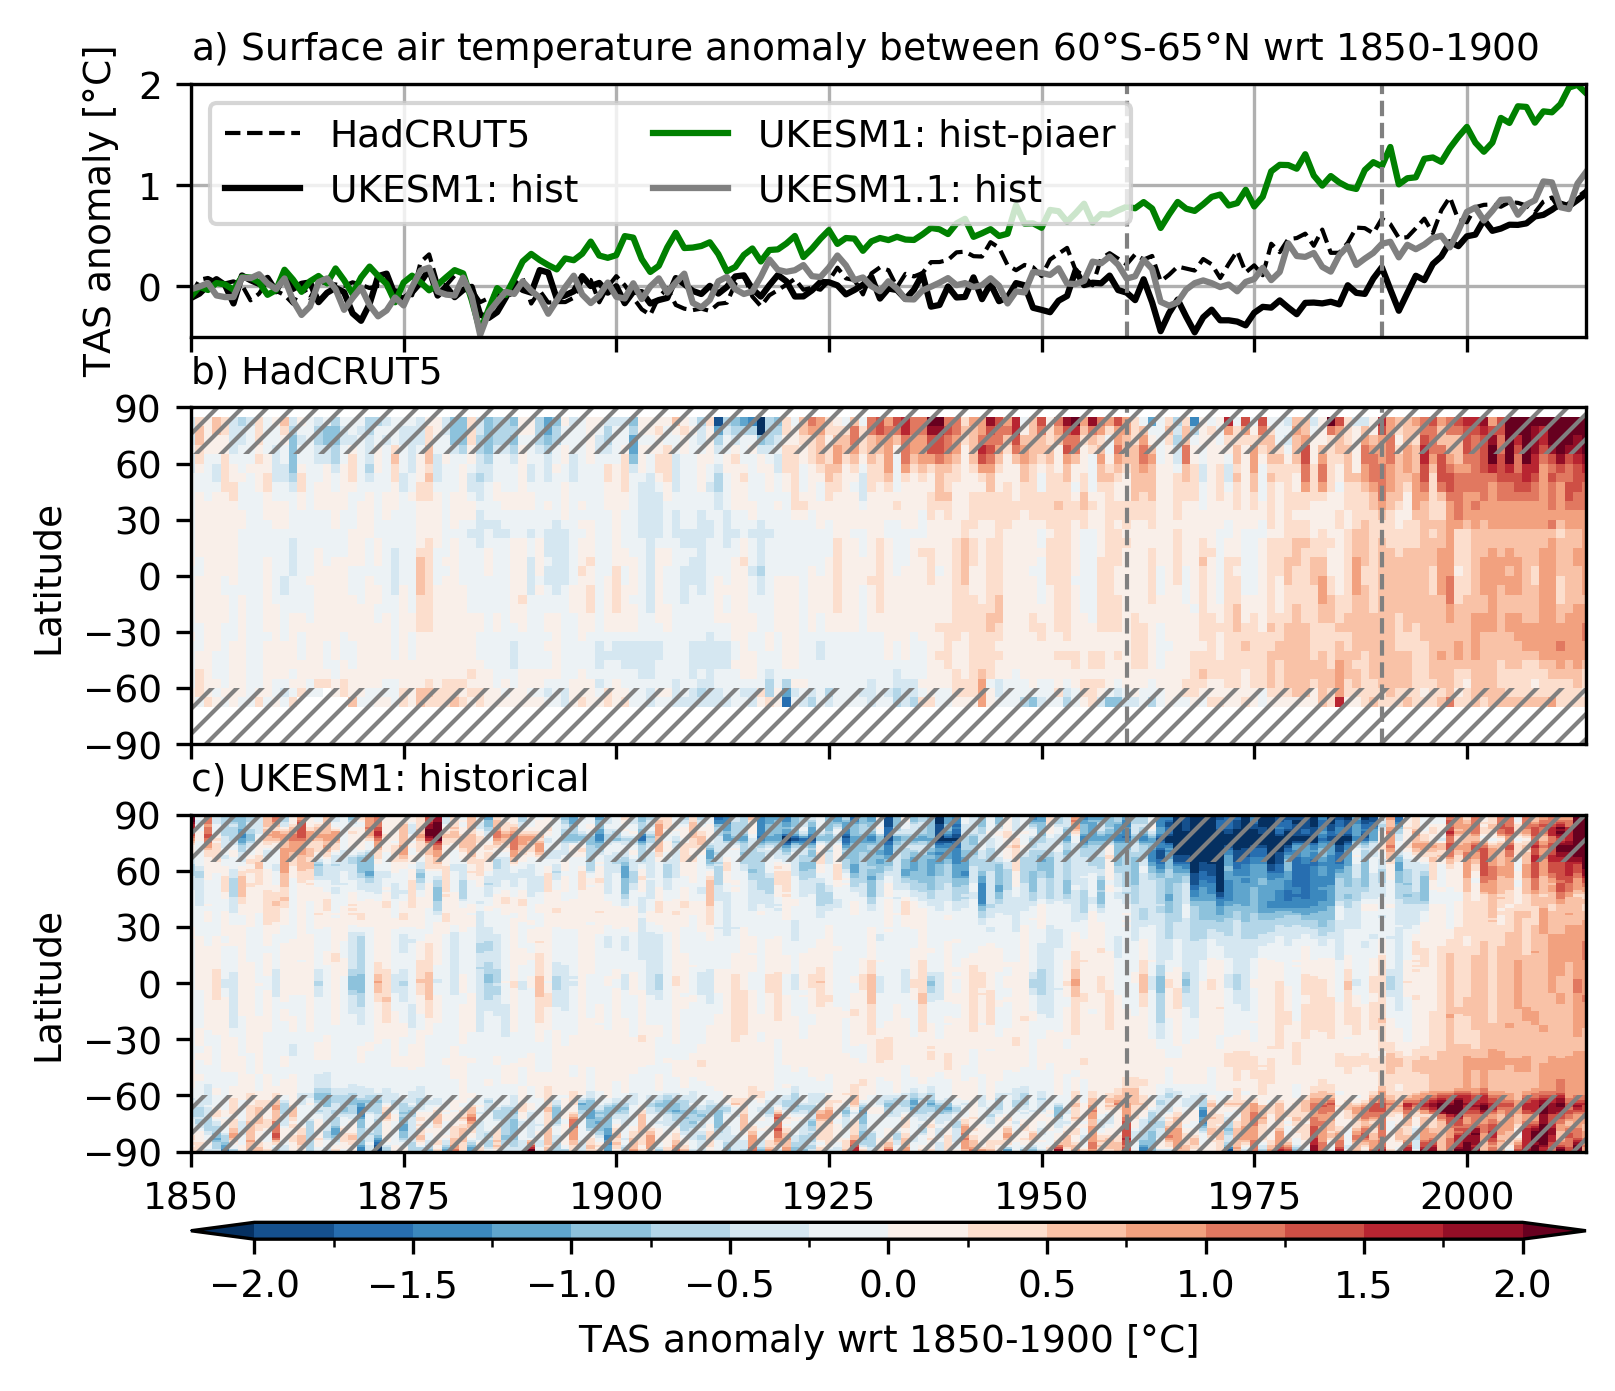
\includegraphics{Appendix1/figs/TAS_anomaly_all.png}
    \caption{Annual mean surface air temperature anomaly between 1850 and 2015 with respect to 1850 and 1900.}
    \label{fig:app1:tas-anomaly-global}
\end{figure}


\include{Appendix2/appendix2}

\end{appendices}

% *************************************** Index ********************************
\printthesisindex % If index is present

\end{document}
